% SPDX-License-Identifier: CC-BY-SA-4.0
%
% Copyright (c) 2020 Philipp Le
%
% Except where otherwise noted, this work is licensed under a
% Creative Commons Attribution-ShareAlike 4.0 License.
%
% Please find the full copy of the licence at:
% https://creativecommons.org/licenses/by-sa/4.0/legalcode


%%%%%%%%%%%%%%%%%%%%%%%%%%%%%%%%%%%%%%%%%%%%%%%%%%%%%%%%%%%
% Configuration
\def\thekindofdocument{Lecture Notes and Exercises}
\def\therevision{1}
\def\therevisiondate{2020-04-27}

%%%%%%%%%%%%%%%%%%%%%%%%%%%%%%%%%%%%%%%%%%%%%%%%%%%%%%%%%%%
% Header
% SPDX-License-Identifier: CC-BY-SA-4.0
%
% Copyright (c) 2020 Philipp Le
%
% Except where otherwise noted, this work is licensed under a
% Creative Commons Attribution-ShareAlike 4.0 License.
%
% Please find the full copy of the licence at:
% https://creativecommons.org/licenses/by-sa/4.0/legalcode

\documentclass[%
	a4paper,%
	twoside,%
	%bibliography=totocnumbered,
	numbers=noenddot,%
	parskip=half,%
	headsepline,%
	footsepline,%
	headings=small,%
	12pt,%
]{scrreprt}

%%%%%%%%%%%%%%%%%%%%%%%%%%%%%%%%%%%%%%%%%%%%%%%%%%%%%%%%%%%%%%%%%%%%%%%%%%%
% Language and fonts
\usepackage[UKenglish]{babel}
\usepackage[utf8]{inputenc}
\usepackage[OT2,T1]{fontenc}
\usepackage{lmodern}
\usepackage{microtype}
\usepackage{array}

%%%%%%%%%%%%%%%%%%%%%%%%%%%%%%%%%%%%%%%%%%%%%%%%%%%%%%%%%%%%%%%%%%%%%%%%%%%
% Graphics

\usepackage{graphicx}
\usepackage{pdfpages}

% TikZ
\usepackage{tikz}
\usepackage{pgf}
\usepackage{pgfplots}
\usepackage{pgfplotstable}
\pgfplotsset{compat=newest}
\pgfplotsset{
	scriptsize/.style={
		width=4.5cm,
		height=,
		legend style={font=\scriptsize},
		tick label style={font=\scriptsize},
		label style={font=\footnotesize},
		title style={font=\footnotesize},
		every axis title shift=0pt,
		max space between ticks=15,
		every mark/.append style={mark size=7},
		major tick length=0.1cm,
		minor tick length=0.066cm,
	},
}
\pgfplotsset{legend cell align=left}
\pgfplotsset{xmajorgrids}
\pgfplotsset{ymajorgrids}
\pgfplotsset{scale only axis}
\pgfplotsset{every axis plot/.append style={line width=1pt}}
\addto\extrasngerman{\pgfplotsset{/pgf/number format/.cd,set decimal separator={{{,}}}}}
\pgfplotsset{/pgf/number format/.cd,1000 sep={\,}}
\usetikzlibrary{positioning}
\usetikzlibrary{shapes.arrows}
\usetikzlibrary{shapes,arrows}
\usetikzlibrary{decorations.pathreplacing}
\usetikzlibrary{math}
\usepackage{pgf-umlsd}

% Circuits
\usepackage[european]{circuitikz}

% Custom TikZ blocks
\tikzset{
	block/.style={
		rectangle,
		align=center,
		minimum height=1cm,
		inner sep=.5cm,
		rounded corners=.15cm
	}
}

% Colours
\usepackage{xcolor}
\usepackage{color}

% Subfigures
\usepackage{subfig}

% Controlling floats
%\renewcommand{\topfraction}{0.8}
%\renewcommand{\bottomfraction}{0.33}
%\renewcommand{\floatpagefraction}{0.66}
%\renewcommand{\textfraction}{0.10}

% Custom functions
\tikzmath{
	function sinc(\x) {
		if  abs(\x) < .001 then { % (|x| < .001) ~ (x = 0)
			return 1;
		} else {
			return sin(\x r)/\x;
		};
	};
}
\tikzmath{
	function asinc(\x, \y) {
		if  abs(\x) < .001 then { % (|x| < .001) ~ (x = 0)
			return 1;
		} else {
			return sin(\y * deg(\x) / 2)/(\y * sin(deg(\x)/2));
		};
	};
}

%%%%%%%%%%%%%%%%%%%%%%%%%%%%%%%%%%%%%%%%%%%%%%%%%%%%%%%%%%%%%%%%%%%%%%%%%%%
% Symbols

\usepackage{textcomp}

% Mathematics
\usepackage{amsmath}
\usepackage{amssymb}
\usepackage{bm}
\usepackage{trsym}

% Quotes
\usepackage{csquotes}

% Formatting units
\usepackage[load-configurations=binary]{siunitx}
\sisetup{per-mode=fraction,mode=math}
\addto\extrasngerman{\sisetup{output-decimal-marker={,}}}
\addto\extrasenglish{\sisetup{output-decimal-marker={.}}}
\addto\extrasngerman{\sisetup{range-phrase={ bis~}}} 
\addto\extrasenglish{\sisetup{range-phrase={ to~}}}

% Cyrillic
\DeclareSymbolFont{cyrletters}{OT2}{wncyr}{m}{n}
\DeclareMathSymbol{\Sha}{\mathalpha}{cyrletters}{"58}

% Custom symbols
%\newcommand{\vect}[1]{\boldsymbol{\vec{\mathbf{#1}}}}
\newcommand{\vect}[1]{\vec{\bm{#1}}}
\newcommand{\cmplxvect}[1]{\vect{\underline{#1}}}
\newcommand{\mat}[1]{\bm{\mathrm{#1}}}
\newcommand{\E}{\mathrm{E}}
\newcommand{\Var}{\mathrm{Var}}
\newcommand{\Cov}{\mathrm{Cov}}
\def\j{\mathsf{j}}

%%%%%%%%%%%%%%%%%%%%%%%%%%%%%%%%%%%%%%%%%%%%%%%%%%%%%%%%%%%%%%%%%%%%%%%%%%%
% Tables

% Lines for Tables
\usepackage{booktabs}

\usepackage{multirow}
\usepackage{longtable}

\usepackage{makecell}

%%%%%%%%%%%%%%%%%%%%%%%%%%%%%%%%%%%%%%%%%%%%%%%%%%%%%%%%%%%%%%%%%%%%%%%%%%%
% Page layout

\usepackage{setspace}
\onehalfspacing

\usepackage[a4paper, margin=2.5cm, headheight=22pt]{geometry}

\usepackage{pdflscape}

\usepackage[bottom]{footmisc}
\interfootnotelinepenalty=10000

% Don't restart footnote count on each chapter
\let\counterwithout\relax
\let\counterwithin\relax
\usepackage{chngcntr}
\counterwithout{footnote}{chapter}
%\usepackage{remreset}
%\makeatletter
%\@removefromreset{footnote}{chapter}
%\makeatother

%%%%%%%%%%%%%%%%%%%%%%%%%%%%%%%%%%%%%%%%%%%%%%%%%%%%%%%%%%%%%%%%%%%%%%%%%%%
% Formatting

\usepackage[normalem]{ulem}

\usepackage{adjustbox}
\usepackage{xspace}
\usepackage{xfrac}
\usepackage{bigfoot}

%\usepackage{float}
%\usepackage{rotating}
\usepackage{rotfloat}

% make \emph{} bold
%\makeatletter
%\DeclareRobustCommand{\em}{%
%  \@nomath\em \if b\expandafter\@car\f@series\@nil
%  \normalfont \else \bfseries \fi}
%\makeatother

%%%%%%%%%%%%%%%%%%%%%%%%%%%%%%%%%%%%%%%%%%%%%%%%%%%%%%%%%%%%%%%%%%%%%%%%%%%
% Bibliography

\usepackage[backend=biber,sorting=none]{biblatex}
\addbibresource{../DCS.bib}

%%%%%%%%%%%%%%%%%%%%%%%%%%%%%%%%%%%%%%%%%%%%%%%%%%%%%%%%%%%%%%%%%%%%%%%%%%%
% Directories

\usepackage[subfigure]{tocloft}

% Acronyms
\usepackage[printonlyused]{acronym}

%\usepackage[xindy,numberedsection,section=section,toc]{glossaries}
%\makeglossaries
%\GlsSetXdyCodePage{duden-utf8}

% Indicies
\usepackage[xindy]{imakeidx}
\makeindex[title=Index]

% ToDo list
\newlistof{todos}{mcf}{To Do}
\newcommand{\todo}[1]{\texttt{\textbf{\#\# TODO \#\# #1 \#\#}} \addcontentsline{mcf}{todos}{#1}}


%%%%%%%%%%%%%%%%%%%%%%%%%%%%%%%%%%%%%%%%%%%%%%%%%%%%%%%%%%%%%%%%%%%%%%%%%%%
% Nomenclature

\usepackage[english]{nomencl}
\makenomenclature
%\usepackage{etoolbox}


\renewcommand\nomgroup[1]{%
	\item[\bfseries
	\ifstrequal{#1}{C}{Physics Constants}{%
		\ifstrequal{#1}{N}{Notation}{%
			\ifstrequal{#1}{S}{Symbols}{%
				\ifstrequal{#1}{F}{Functions}{%
					\ifstrequal{#1}{B}{Block Symbols}{%
					}%
				}%
			}%
		}%
	}%
]}

\newcommand{\nomunit}[1]{%
	\renewcommand{\nomentryend}{\hspace*{\fill}#1}}

\nomenclature[C]{$c$}{Speed of light}

\nomenclature[Na]{$\underline{a}$}{Value, explicitly marked complex valued}
\nomenclature[Nb]{$\vect{a}$}{Vector}
\nomenclature[Nba]{$\vect{\underline{a}}$}{Vector, explicitly marked complex valued}
\nomenclature[Nc]{$\mat{A}$}{Matrix}
\nomenclature[Nca]{$\mat{\underline{A}}$}{Matrix, explicitly marked complex valued}
\nomenclature[Nxa]{$\underline{x}(t)$}{Analog signal in time domain}
\nomenclature[Nxb]{$\underline{X}(\j \omega)$}{Analog signal in frequency domain (Fourier transform)}
\nomenclature[Nxb]{$\underline{X}(\underline{s})$}{Analog signal in frequency domain (Laplace transform)}
\nomenclature[Nxc]{$\underline{x}[k] = \underline{x}\left(k T_S\right)$}{Digital signal in time domain, with sampling period $T_S$}
\nomenclature[Nxd]{$\underline{X}(\underline{z})$}{Digital signal in frequency domain (z-transform)}

%%%%%%%%%%%%%%%%%%%%%%%%%%%%%%%%%%%%%%%%%%%%%%%%%%%%%%%%%%%%%%%%%%%%%%%%%%%
% Listings

\usepackage{listings}


%%%%%%%%%%%%%%%%%%%%%%%%%%%%%%%%%%%%%%%%%%%%%%%%%%%%%%%%%%%%%%%%%%%%%%%%%%%
% Exercises

\usepackage{exsheets}
\SetupExSheets{
	headings = block-subtitle,
	headings-format = \bfseries\sffamily,
	subtitle-format = \bfseries\sffamily,
	counter-within = chapter,
	counter-format = ch.qu\IfQuestionSubtitleT{:},
	toc-level = {subsection},
	% solution/print = true % uncomment for tutors
}

%%%%%%%%%%%%%%%%%%%%%%%%%%%%%%%%%%%%%%%%%%%%%%%%%%%%%%%%%%%%%%%%%%%%%%%%%%%
% PDF Metadata

\def\hyperrefgeneraltitle{Digital Communication Systems - \thekindofdocument{}}
\ifdefined\thesubtitle
\def\hyperreftitle{\hyperrefgeneraltitle{} - \thesubtitle{}}
\else
\def\hyperreftitle{\hyperrefgeneraltitle{}}
\fi

\usepackage[
	pdftitle={\hyperreftitle{}},
	pdfauthor={Philipp Le},
	pdfcreator={LaTeX with hyperref and KOMA-Script},
	pdfsubject={},
	pdfkeywords={},
	pdfstartview={Fit},
	pdflang={en-GB},
	pdfduplex={DuplexFlipLongEdge}
	hidelinks]{hyperref}


%%%%%%%%%%%%%%%%%%%%%%%%%%%%%%%%%%%%%%%%%%%%%%%%%%%%%%%%%%%%%%%%%%%%%%%%%%%
% Own commands

\newcommand{\licensequote}[3]{\textit{Reproduced from #1. Copyright by #2. License: #3.}}


%%%%%%%%%%%%%%%%%%%%%%%%%%%%%%%%%%%%%%%%%%%%%%%%%%%%%%%%%%%%%%%%%%%%%%%%%%%
% Own environments

\usepackage{tcolorbox}
\tcbuselibrary{breakable, skins}

\newenvironment{attention}{%
	\begin{tcolorbox}[colframe=red]%
	{\sffamily\bfseries Attention!}\par%
}{%
	\end{tcolorbox}%
}

\newenvironment{definition}[1]{%
	\begin{tcolorbox}[enhanced jigsaw, breakable, colframe=gray]%
	{\sffamily\bfseries Definition: #1}\par%
}{%
	\end{tcolorbox}%
}

\newenvironment{fact}{%
	\begin{tcolorbox}[colframe=gray!80]%
	\bfseries%
}{%
	\end{tcolorbox}%
}

\newenvironment{proof}[1]{%
	\begin{tcolorbox}[enhanced jigsaw, breakable, colframe=black]%
	{\sffamily\bfseries Proof: #1}\par%
}{%
	\end{tcolorbox}%
}

\newenvironment{derivation}[1]{%
	\begin{tcolorbox}[enhanced jigsaw, breakable, colframe=black]%
	{\sffamily\bfseries Derivation: #1}\par%
}{%
	\end{tcolorbox}%
}

\newenvironment{example}[1]{%
	\begin{tcolorbox}[enhanced jigsaw, breakable, colframe=black!60]%
	{\sffamily\bfseries Example: #1}\par%
}{%
	\end{tcolorbox}%
}

\newenvironment{excursus}[1]{%
	\begin{tcolorbox}[enhanced jigsaw, breakable, colframe=gray!40]%
	{\sffamily\bfseries Excursus: #1}\par%
}{%
	\end{tcolorbox}%
}




\begin{document}

%%%%%%%%%%%%%%%%%%%%%%%%%%%%%%%%%%%%%%%%%%%%%%%%%%%%%%%%%%%
% Title Page
\pagenumbering{Alph}
\pagestyle{empty}

% Title Page
% SPDX-License-Identifier: CC-BY-SA-4.0
%
% Copyright (c) 2020 Philipp Le
%
% Except where otherwise noted, this work is licensed under a
% Creative Commons Attribution-ShareAlike 4.0 License.
%
% Please find the full copy of the licence at:
% https://creativecommons.org/licenses/by-sa/4.0/legalcode

\begin{titlepage}
	\begin{center}
		\normalsize

		\vspace*{1cm}
	
		
\includegraphics[width=9cm]{../common/EIT_SIGN_ovgu}
		
		\vspace{1.5cm}
	
		\Huge
		Digital Communication Systems
		
		\vspace{0.75cm}
		
		\ifdefined\thesubtitle
		\Large
		\thesubtitle
		
		\vspace{0.75cm}
		\par
		\fi
		
		\normalsize
		\textbf{\thekindofdocument}
		
		\vspace{1.5cm}
		
		\normalsize
		Chair of Microwave and Communication Engineering \\
		Institute for Information Technology and Communications \\
		Faculty of Electrical Engineering and Information Technology \\
		Otto-von-Guericke-University Magdeburg
		
		\vspace{0.75cm}

		\normalsize
		\textsc{Lecturer:} \\
		Philipp Le, M.\,Sc.
		
		\vspace{0.75cm}
		
		\normalsize
		Summer Semester 2023
	\end{center}

	\vfill
	
	\begin{flushright}
		\footnotesize
		Serial number \VcsCommitNo, \VcsCommitDate
	\end{flushright}
\end{titlepage}

\newpage

%%%%%%%%%%%%%%%%%%%%%%%%%%%%%%%%%%%%%%%%%%%%%%%%%%%%%%%%%%%
% Preface
\pagenumbering{arabic}
\pagestyle{headings}

% Inhaltsverzeichnis
%\tableofcontents
%\newpage

% Imprint
% SPDX-License-Identifier: CC-BY-SA-4.0
%
% Copyright (c) 2020 Philipp Le
%
% Except where otherwise noted, this work is licensed under a
% Creative Commons Attribution-ShareAlike 4.0 License.
%
% Please find the full copy of the licence at:
% https://creativecommons.org/licenses/by-sa/4.0/legalcode

\phantomsection
\chapter*{Imprint}

{
\small

License:

\begin{quote}
	\includegraphics[width=2cm]{svg/cc-by-sa-4-0.pdf}
		
	Copyright \textcopyright{} 2020 Philipp Le
	
	Except where otherwise noted, this work is licensed under a
	Creative Commons Attribution-ShareAlike 4.0 License.
	
	Please find the full copy of the licence at \url{https://creativecommons.org/licenses/by-sa/4.0/legalcode}.
	
	A short, but legally non-binding deed of the licence is at \url{https://creativecommons.org/licenses/by-sa/4.0/}.
\end{quote}

\vspace{1.5em}

\hrule{}

\vspace{1.5em}

\LaTeX{} sources at \url{https://github.com/pl33/dcs-lecture-notes}.

\vspace{1.5em}

\hrule{}

\vspace{1.5em}

Information according to the Press Law of the Land Saxony-Anhalt:\\
Angaben gem\"a{}{\ss} des Pressegesetzes des Landes Sachsen-Anhalt:

Verfasser, V.i.S.d.P: Philipp Le, Pablo-Neruda-Str. 6, 39126 Magdeburg

}

\newpage

% Abstract
% SPDX-License-Identifier: CC-BY-SA-4.0
%
% Copyright (c) 2020 Philipp Le
%
% Except where otherwise noted, this work is licensed under a
% Creative Commons Attribution-ShareAlike 4.0 License.
%
% Please find the full copy of the licence at:
% https://creativecommons.org/licenses/by-sa/4.0/legalcode

\phantomsection
\addcontentsline{toc}{chapter}{Abstract}
\chapter*{Abstract}

The course covers the properties and functions of digital communication systems. The first part provides a recap on signal description in the time-domain and frequency-domain, stochastic and deterministic signal, and digital signal processing. Based on these foundations, various aspects of modern digital communication are considered. The concept of noise is introduced. System components of communication systems (mixers, filters, etc.) are discussed. Spread spectrum and channel access technologies are introduced (OFDM, CDMA, …). Basics of information theory and coding are considered as well as challenges of communication over wireless transmission channels.

\textit{Keywords} -- digital communication, communication system, signal processing, spread spectrum, multiple access, wireless communication, OFDM, CMDA, information theory, coding

\newpage

\phantomsection
\addcontentsline{toc}{chapter}{Contents}
\tableofcontents
\clearpage

% List of Acronyms
% SPDX-License-Identifier: CC-BY-SA-4.0
%
% Copyright (c) 2020 Philipp Le
%
% Except where otherwise noted, this work is licensed under a
% Creative Commons Attribution-ShareAlike 4.0 License.
%
% Please find the full copy of the licence at:
% https://creativecommons.org/licenses/by-sa/4.0/legalcode

\phantomsection
\addcontentsline{toc}{chapter}{List of Abbreviations}
\chapter*{List of Abbreviations}

\begin{acronym}[blablablabla]
	\acro{ADC}{analog-to-digital converter}
	\acro{AM}{amplitude modulation}
	\acro{AOA}{angle of arrival}
	\acro{AWGN}{additive white Gaussian noise}
	\acro{ASIC}{application-specific integrated circuit}
	\acro{ASK}{amplitude-shift keying}
	\acro{B2B}{business-to-business}
	\acro{BER}{bit error rate}
	\acro{BIBO}{bounded-input, bounded-output}
	\acro{BPF}{band pass filter}
	\acro{BPM}{burst-position modulation}
	\acro{BPSK}{binary phase-shift keying}
	\acro{BS}{base station}
	\acro{BSF}{band stop filter}
	\acro{CDF}{cummulative distribution function}
	\acro{CDM}{code-division multiplexing}
	\acro{CDMA}{code-division multiple access}
	\acro{CEP}{circular error probablilty}
	\acro{CFR}{channel frequency response}
	\acro{CIC}{cascaded integrator-comb}
	\acro{CIR}{channel impulse response}
	\acro{CMF}{channel matched filter}
	\acro{CPU}{central processing unit}
	\acro{CRLB}{Cramer-Rao lower bound}
	\acro{CSMA-CA}{carrier sense multiple access collision avoidance}
	\acro{CTFT}{continuous-time Fourier transform}
	\acro{CW}{continuous wave}
	\acro{DAC}{digital-to-analog converter}
	\acro{DC}{discrete current}
	\acro{DFT}{discrete Fourier transform}
	\acro{DME}{Distance Measuring Equipment}
	\acro{DOP}{dilution of precision}
	\acro{DPSK}{differential phase-shift keying}
	\acro{DSB}{double-sideband}
	\acro{DSB-TC}{double-sideband transmitted carrier}
	\acro{DSB-SC}{double-sideband suppressed carrier}
	\acro{DSP}{digital signal processor}
	\acro{DSSS}{direct-sequence spread spectrum}
	\acro{DS-CDMA}{direct sequence code-division multiple access}
	\acro{DTFT}{discrete-time Fourier transform}
	\acro{EHF}{extremely high frequency}
	\acro{EIRP}{effective isotropic radiated power}
	\acro{ELF}{extremely low frequency}
	\acro{EMC}{electromagnetic compatibility}
	\acro{ENOB}{effective number of bits}
	\acro{ETSI}{European Telecommunications Standards Institue}
	\acro{FCC}{Federal Communications Commission}
	\acro{FEC}{forward error correction}
	\acro{FDL}{field bus data link}
	\acro{FDP}{first detected path}
	\acro{FDD}{frequency-division duplex}
	\acro{FDM}{frequency-division multiplexing}
	\acro{FDMA}{frequency-division multiple access}
	\acro{FEC}{forward error coding}
	\acro{FFT}{fast Fourier transform}
	\acro{FH-CDMA}{frequency-hopping code-division multiple access}
	\acro{FHSS}{frequency-hopping spread spectrum}
	\acro{FIR}{finite impulse response}
	\acro{FPGA}{field-programmable gate array}
	\acro{FSPL}{free-space path loss}
	\acro{FWHM}{full width at half maximum}
	\acro{GIS}{Geo Information System}
	\acro{GNSS}{global navigation satellite system}
	\acro{GPIO}{general-purpose input and output}
	\acro{GPS}{Global Positioning System}
	\acro{GSM}{Global System for Mobile Communications}
	\acro{HDL}{hardware description language}
	\acro{HF}{high frequency}
	\acro{HPF}{high pass filter}
	\acro{HTTP}{Hypertext Transfer Protocol}
	\acro{I}{in-phase}
	\acro{IC}{integrated circuit}
	\acro{ID}{identification}
	\acro{IEEE}{Institute of Electrical and Electronics Engineers}
	\acro{IETF}{Internet Engineering Task Force}
	\acro{IF}{intermediate frequency}
	\acro{IFFT}{inverse fast Fourier transform}
	\acro{IIR}{infinite impulse response}
	\acro{IOT}{Intenet of Things}
	\acro{IP}{Internet Protocol}
	\acro{IR}{impulse radio}
	\acro{ISI}{inter-symbol interference}
	\acro{ISM}{industrial, scientific and medical}
	\acro{ITU}{International Telecommunication Union}
	\acro{LBS}{location based service}
	\acro{LF}{low frequency}
	\acro{LFSR}{linear feedback shift register}
	\acro{LNA}{low noise amplifier}
	\acro{LO}{local oscillator}
	\acro{LORAN-C}{Long Range Navigation-C}
	\acro{LOS}{line-of-sight}
	\acro{LPF}{low pass filter}
	\acro{LS}{least squares}
	\acro{LSB}{least significant bit}
	\acro{LTE}{Long Term Evolution}
	\acro{LTI}{linear, time-invariant}
	\acro{LVPECL}{low-voltage positive emitter-coupled logic}
	\acro{MAC}{medium access control}
	\acro{MAP}{maximum aposteriori}
	\acro{MB-OFDM}{multiband orthogonal frequency-division multiplexing}
	\acro{MCU}{micro-controller unit}
	\acro{MF}{medium frequency}
	\acro{ML}{maximum likelihood}
	\acro{MSB}{most significant bit}
	\acro{MSE}{mean square error}
	\acro{MMSE}{minimum mean square error}
	\acro{MQTT}{message queuing telemetry transport}
	\acro{MU}{mobile unit}
	\acro{NCO}{nummerically-controlled oscillator}
	\acro{NLOS}{non-line-of-sight}
	\acro{OFDM}{orthogonal frequency-division multiplexing}
	\acro{OFDMA}{orthogonal frequency-division multiple access}
	\acro{OOK}{on-off keying}
	\acro{OSI}{Open Systems Interconntection}
	\acro{OVSF}{orthogonal variable spreading factor}
	\acro{PAN}{personal area network}
	\acro{PC}{personal computer}
	\acro{PCM}{pulse-code modulation}
	\acro{PCB}{printed circuit board}
	\acro{PDF}{probability density function}
	\acro{PHR}{physical layer header}
	\acro{PHY}{physical layer}
	\acro{PLD}{programmable logic device}
	\acro{PLL}{phase-locked loop}
	\acro{PM}{phase modulation}
	\acro{PRN}{pseudo-random noise}
	\acro{PPDU}{physical layer protocol data unit}
	\acro{PPM}{pulse-position modulation}
	\acro{PRF}{pulse repetition frequency}
	\acro{PSD}{power spectral density}
	\acro{PSDU}{physical layer service data unit}
	\acro{PSK}{phase-shift keying}
	\acro{Q}{quadrature}
	\acro{QAM}{quadrature amplitude modulation}
	\acro{QED}{quod erat demonstrandum}
	\acro{QOS}{quality of service}
	\acro{QPSK}{quadrature phase-shift keying}
	\acro{RAM}{random access memory}
	\acro{ROM}{read-only memory}
	\acro{RS}{recommended standard}
	\acro{RTC}{real-time clock}
	\acro{QAM}{quadrature amplitude modulation}
	\acro{QPSK}{quadrature phase shift keying}
	\acro{RF}{radio frequency}
	\acro{RFID}{radio frequency identification}
	\acro{RMS}{root mean square}
	\acro{RSSI}{received signal strength indication}
	\acro{RTLS}{real-time localization system}
	\acro{RTT}{round trip time}
	\acro{SAP}{service access point}
	\acro{SDM}{space-division multiplexing}
	\acro{SDMA}{space-division multiple access}
	\acro{SDR}{software-defined radio}
	\acro{SECDED}{single error correct, double error detect}
	\acro{SEP}{spherical error probablilty}
	\acro{SFD}{start of frame delimiter}
	\acro{SHF}{super high frequency}
	\acro{SLF}{super low frequency}
	\acro{SNR}{signal-to-noise ratio}
	\acro{SQNR}{signal-to-qunatization-noise ratio}
	\acro{SPI}{serial peripheral interface}
	\acro{SSB}{single-sideband}
	\acro{SSB-SC}{single-sideband suppressed carrier}
	\acro{TCXO}{temperature-compensated crystal oscillator}
	\acro{TCP}{Transmission Control Protocol}
	\acro{TETRA}{Terrestrial Trunked Radio}
	\acro{THSS}{time-hopping spread spectrum}
	\acro{TH-CDMA}{time-hopping code-division multiple access}
	\acro{TOA}{time of arrival}
	\acro{TDD}{time-division duplex}
	\acro{TDM}{time-division multiplexing}
	\acro{TDMA}{time-division multiple access}
	\acro{TD-CDMA}{time-division code-division multiple access}
	\acro{TDOA}{time difference of arrival}
	\acro{UART}{universal asynchronous receiver and transmitter}
	\acro{UDP}{user datagram protocol}
	\acro{UDP}{User Datagram Protocol}
	\acro{UERE}{user equivalent range error}
	\acro{UHF}{ultra high frequency}
	\acro{ULF}{ultra low frequency}
	\acro{UMTS}{Universal Mobile Telecommunications System}
	\acro{UN}{United Nations}
	\acro{USB}{Universal Serial Bus}
	\acro{UTC}{Coordinated Universal Time}
	\acro{UWB}{ultra-wide band}
	\acro{VCO}{voltage controlled oscillator}
	\acro{VHF}{very high frequency}
	\acro{VLF}{very low frequency}
	\acro{VOR}{VHF Omnidirectional Range}
	\acro{WLAN}{wireless local area network}
	\acro{WPAN}{wireless personal area network}
	\acro{WSS}{wide sense stationary}
\end{acronym}
\newpage

% Nomenclature
\phantomsection
\addcontentsline{toc}{chapter}{Nomenclature}
\printnomenclature
\newpage

%%%%%%%%%%%%%%%%%%%%%%%%%%%%%%%%%%%%%%%%%%%%%%%%%%%%%%%%%%%
% Content

\phantomsection
\addcontentsline{toc}{chapter}{Preface: Digital Communication -- A Future Technology}
\chapter*{Preface: Digital Communication -- A Future Technology}

\begin{refsection}

The current time during the Corona lockdown shows the great significance of telecommunication. It is self-evident to have access to online media and communication platforms. The internet helps to keep in touch with our loved ones. A huge amount of entertainment relies on internet access. The internet is highly integrated in our every-day life. Furthermore, it is a growing economy. There are not only the online services like social media or online warehouses which are going to expand their business in the future. The communication technologies, which the internet is built upon, are a growing and innovative market, too. Besides consumers, the \ac{B2B} market is a huge driver of innovation. It must be expected, that more devices get interconnected. This is a challenge because physical resources are limited. Nevertheless, it is a great possibility for the communication technology to advance. The technologies, which are able to cope with the new requirementes, are digital. This where the course on \emph{Digital Communication Systems} starts. You are warmly welcomed!

\addcontentsline{toc}{section}{History of Communications}
\section*{History of Communications}

Let's go back to the roots! Communication is the most important property of human beings. The spoken language has always been the most important instrument of communication between human.

An early innovation in communication technology is the written language. Information can now be conserved for a long time and even be transferred to other places. Modern societies would not be possible without written language.

Transferring information became more important as societies advanced.
\begin{itemize}
	\item People all over the world used drums or other devices to generate sounds.
	\item Some Native Americans tribes used smoke signs to communicate over large distances.
	\item The invention of paper simplified communication. Large amount of information could be stored and transferred.
	\item An example of more sophisticated communication technology is the \index{Caesar cipher} Caesar cipher used in the Roman Empire in ancient times. It is one of the first devices developed for cryptography.
	\item Homing pigeons delivered letters over long distances.
	\item In the Middle Ages, beacons were used in defensive communication to relay a signal.
	\item In the 18th century, semaphore lines had been built. They used visual telegraphy. Semaphores on fixed towers could display a set of symbols, which were relayed along the line.
\end{itemize}

\begin{minipage}{0.45\linewidth}
	\begin{figure}[H]
		\centering
		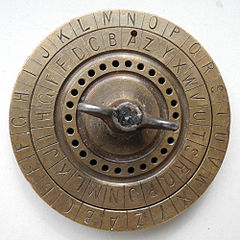
\includegraphics[width=\linewidth]{../chapter00/CaesarCipher.jpg}
		\caption[Caesar cipher]{Caesar cipher. Each letter is replaced by another one which is a fixed number of letters away from the original one. \licensequote{\cite{Berberich2013}}{Hubert Berberich}{Public Domain}}
	\end{figure}
\end{minipage}
\hfill
\begin{minipage}{0.45\linewidth}
	\begin{figure}[H]
		\centering
		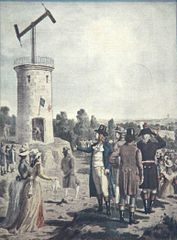
\includegraphics[width=\linewidth]{../chapter00/OpticalTelegraph.jpg}
		\caption[Optical telegraph]{Optical telegraph \cite{WikiSemaphore}}
	\end{figure}
\end{minipage}

The research of electricity created the foundations for modern communication systems. Electrical telegraphy speeded up telecommunication. At the end of the 19th century, electromagnetic waves have been discovered. James Clerk Maxwell postulated them in 1865. Heinrich Hertz produced the first electromagnetic waves in 1887. The potential had soon been acknowledged by inventors, who developed first radios. The era of analogue radio communication began. The \index{vacuum tube} vacuum tube became an important component in radio electronics.

In 1947, the bipolar transistor had been invented. This marked the beginning of the semiconductor era, which still endures. Over the decades, semiconductors became more integrated. In 1958, the first \ac{IC} had been demonstrated by Jack Kilby, engineer at Texas Instruments. At this time, wireless communication was mostly restricted to broadcasting and professional users.

With the 1990s, wireless communication technologies became more and more affordable for private usage. Advancing computer since was incorporated into communication systems. Digital communication systems gained significance and started superseding analogue communication technologies.

\addcontentsline{toc}{section}{An Innovation Motor}
\section*{An Innovation Motor}

Nowadays, innovations are driven by the demand for telecommunication which especially
\begin{itemize}
	\item is fast,
	\item is reliable,
	\item is secure,
	\item has higher throughput, and
	\item reduces the cost.
\end{itemize}

Speed and data rate are important measures, which are advertised by companies selling their products. For example, the entertainment industry like video-on-demand services require more bandwidth to deliver video streams of higher quality. Stock exchanges need low latency to trade securities within milliseconds.

Reliability is a key requirement for critical infrastructure. An unreliable system may result in loss of production or may even lead to serious dangers for health and life of people. For example, railroad traffic management requires extremely reliable communication systems for high-speed trains to prevent accidents. This goes along with security. Unauthorized parties shall have no access to the communication system. Data integrity and privacy are important.

There is often a trade-off between different requirements. No technology can fit all requirements equally. The greatest challenge for an engineer, working on Digital Communications Systems, is finding the optimal solution, which fits the customer's wishes best.

As a general rule, cost reduction is the main argument for businesses to adapt new technologies. Other requirements must of course fit. However, technologies are unlike to be implemented if they increase the monetary costs for the user.


\addcontentsline{toc}{section}{Unlimited Possibilities}
\section*{Unlimited Possibilities}

Each interconnected electronic component is a communication system. Even if a device does not communicate with its environment, its interconnected components may exchange data with each other. This shows the significance of digital communication systems. In addition, many devices provide a digital communication interface or radio link to interconnect with other devices.

Understanding digital communication systems is of great importance in many engineering and non-engineering fields, for example:
\begin{itemize}
	\item \textbf{Automation} -- 
	\item \textbf{Medical Systems} -- 
	\item \textbf{Transport} -- railway, air traffic
	\item \textbf{Public Safety} -- 
	\item \textbf{Agriculture} -- 
	\item \textbf{Energy Sector} -- 
\end{itemize}

\printbibliography[heading=subbibliography]
\end{refsection}

\clearpage

\setcounter{chapter}{-1}

\phantomsection
\addcontentsline{toc}{section}{Exercise 0 - Warm Up}
\section*{Exercise 0 -- Warm Up}

Make up your mind of communication technologies and how they can be used. This exercise does not cover the actual course content, but shall give you an introduction to the topic of \emph{digital communication systems}.

\begin{question}
	Name 5 communication devices of your every-day life!
\end{question}

\begin{solution}
	\begin{itemize}
		\item Cell phone (Wifi, 4G, Bluetooth)
		\item TV
		\item PC (Wifi, Ethernet, Bluetooth)
		\item Access control key fob
		\item Bluetooth headset
	\end{itemize}
\end{solution}

\begin{question}
	Name 5 possible areas of application for digital communication systems! Describe them briefly!
\end{question}
\clearpage

\setcounter{chapter}{0}

\chapter{Communication Systems}

\begin{refsection}

\section{What is Communication?}

\index{communication}
\textbf{Communication} (from Latin \emph{communicare}, ``to share'') is the act of conveying information from one entity to another using mutually understood sign and symbols.

\index{information}
\textbf{Information} is the knowledge which is being conveyed from the source to the recipient. Information results in increased knowledge at the recipient's side.

Many research areas concern with communication and information:
\begin{itemize}
	\item Information theory: Quantification, storage, communication and information in general
	\item Communication studies: Human communication
	\item Linguistics: Language as a carrier of information
	\item Biosemiotics: Communication in and between living organisms
	\item ...
\end{itemize}

Communication and information are general terms. \textbf{Digital communication} concerns with the technology of conveying information using discrete signals. A \textbf{digital communication system} is a set of components and processes which implement digital communication. The signals carrying the information in a digital communication system are usually electromagnetic waves.


\section{Objectives and Distinction from Other Subjects}

This course will provide an understanding of how a digital communication system can be described. You will learn methods to describe information in their physical form as signals as well as system components. 

The theory of digital communication system is strongly connected to other subjects, for example:
\begin{itemize}
	\item Information and coding theory
	\item Computer networks
	\item Statistics
	\item Signals and systems
	\item Microwave engineering
	\item Electronics
\end{itemize}
There are courses at this university which give you a deeper insight into these subjects.


\section{Components of A Communication System}


\subsection{Communication Model}

%\todo{citation}
Claude Shannon and Warren Weaver were engineers at the Bell Telephone Labs, USA. They developed the \index{Shannon-Weaver model} \textbf{Shannon-Weaver Model} \cite{Shannon1949} (Figure \ref{fig:ch01:shannon_weaver_model}).

\begin{figure}[H]
	\centering
	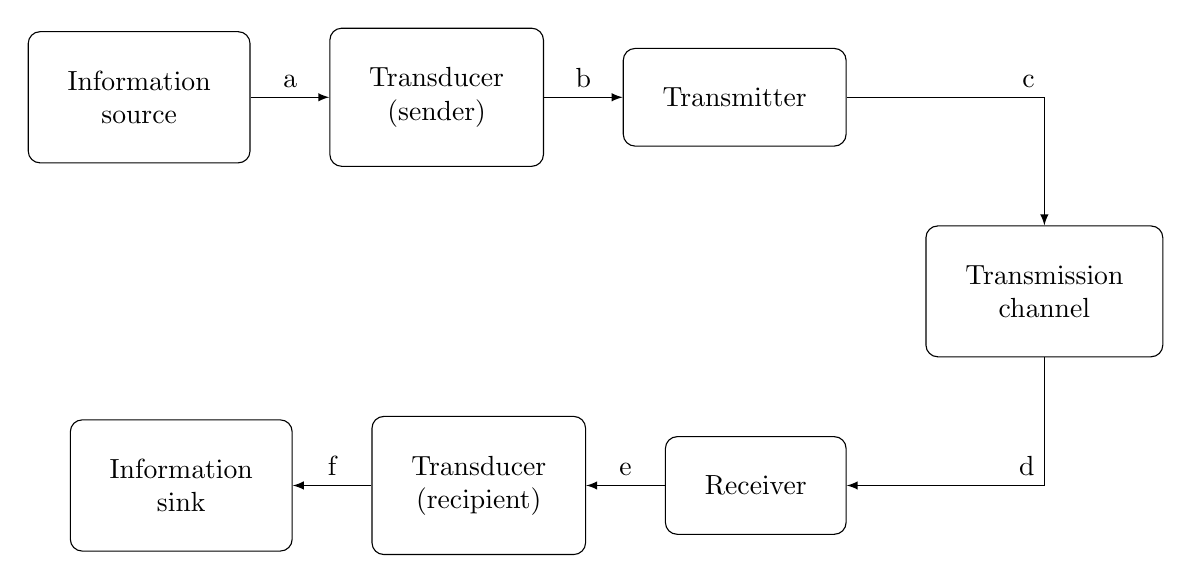
\begin{tikzpicture}
		\draw node[draw, block](Source){Information\\ source};
		\draw node[draw, block, right=of Source](STrans){Transducer\\ (sender)};
		\draw node[draw, block, right=of STrans](TX){Transmitter};
		\draw node[draw, block, below right=of TX](Ch){Transmission\\ channel};
		\draw node[draw, block, below left=of Ch](RX){Receiver};
		\draw node[draw, block, left=of RX](RTrans){Transducer\\ (recipient)};
		\draw node[draw, block, left=of RTrans](Sink){Information\\ sink};
		
		\draw[-latex] (Source) -- node[midway, align=center, above]{a} (STrans);
		\draw[-latex] (STrans) -- node[midway, align=center, above]{b} (TX);
		\draw[-latex] (TX) -| node[midway, align=center, above left]{c} (Ch);
		\draw[-latex] (Ch) |- node[midway, align=center, above left]{d} (RX);
		\draw[-latex] (RX) -- node[midway, align=center, above]{e} (RTrans);
		\draw[-latex] (RTrans) -- node[midway, align=center, above]{f} (Sink);
	\end{tikzpicture}
	\caption{Shannon-Weaver model of communication}
	\label{fig:ch01:shannon_weaver_model}
\end{figure}

\begin{description}
	\item[Information source] The information is created here.
	\item[Signal a] The original information is represented in physical form by a signal.
	\item[Transducer (sender)] The \index{Shannon-Weaver model!transducer} transducer converts the signal from one physical form to another.
	\item[Signal b] The signal is in a form which can be processed by the transmitter.
	\item[Transmitter] The information is modulated on a carrier, which can be transmitted through the transmission channel.
	\item[Signal c] The information is modulated on a carrier and can pass through the transmission channel.
	\item[Tansmission channel] The physical system through which the modulated information passes. \index{transmission channels} Transmission channels are noisy and add disturbances to the information.
	\item[Signal d] It is basically the Signal c. However, noise and disturbances have been added.
	\item[Receiver] The receiver extracts the information from the carrier. Information must be reconstructed from the noisy input signal.
	\item[Signal e] The output signal of the receiver.
	\item[Transducer (recipient)] The signal must be converted into a physical form which can be processed by the information sink.
	\item[Signal f] The signal carries the information in a form which can be used by the information sink.
	\item[Information sink] The endpoint of the information. It uses the information to gain knowledge.
\end{description}

\paragraph{Example: Cell phone}

\begin{enumerate}
	\item The information source is the brain.
	\item Electrical impulses and molecules are conveyed by the nerves to the vocal cords (transducer 1). Vocal cords convert the signals to sound.
	\item The sound is converted to an electrical signal by a microphone (transducer 2).
	\item The electrical pulses are modulated on a radio carrier (transmitter).
	\item Radio waves are transmitted over the air (transmission channel).
	\item A noisy signal is received. The receivers demodulates the information from the radio carrier.
	\item The analogue electrical signal is converted into sound by a speaker (transducer 3).
	\item The sound reaches the ear that converts them to electrical pulses (transducer 4).
	\item Electrical impulses and molecules are conveyed by the nerves to the brain (information sink).
\end{enumerate}


\subsection{Classification of Signals}

A \index{signal} signal conveys information in a form that can be processed by components of the communication systems.

\begin{figure}[H]
	\centering
	\begin{tikzpicture}
		\draw node[block](Main){\textbf{Signals carrying}\\ \textbf{information}};
		\draw node[block, below left=of Main](Analogue){Analogue};
		\draw node[block, below right=of Main](Digital){Digital};
		\draw node[block, below left=of Analogue](TimeCont){Time\\ continuous};
		\draw node[block, below right=of Analogue](TimeDis){Time\\ discrete};
		
		\draw [-latex] (Main) -- (Analogue);
		\draw [-latex] (Main) -- (Digital);
		\draw [-latex] (Analogue) -- (TimeCont);
		\draw [-latex] (Analogue) -- (TimeDis);
	\end{tikzpicture}
	\caption{Classification of signals carrying information}
	\label{fig:ch01:signals_classif}
\end{figure}

\paragraph{Analogue signals.}

\index{signal!analogue signal}
\index{signal!value-continuous}
Analogue signals are represented by values out of a continuous range (\emph{value-continuous}). The range can be limited. However, each real value in this range can be taken.

Examples:
\begin{itemize}
	\item Acoustic signals (speech, sound)
	\item Electric signals (voltage, current)
	\item Light signals (microscope, photograph)
\end{itemize}

\index{signal!time-continuous}
\index{signal!time-discrete}
Analogue signals can be time-continuous or time-discrete. \emph{Time-continuity} means that the signal is defined at any real point of time. A \emph{time-discrete} signal is only defined at certain time instances. The number of time instances can be unlimited. However, the signal is not defined between two time points.

\begin{figure}[H]
	\centering
	\begin{adjustbox}{scale=0.8}
		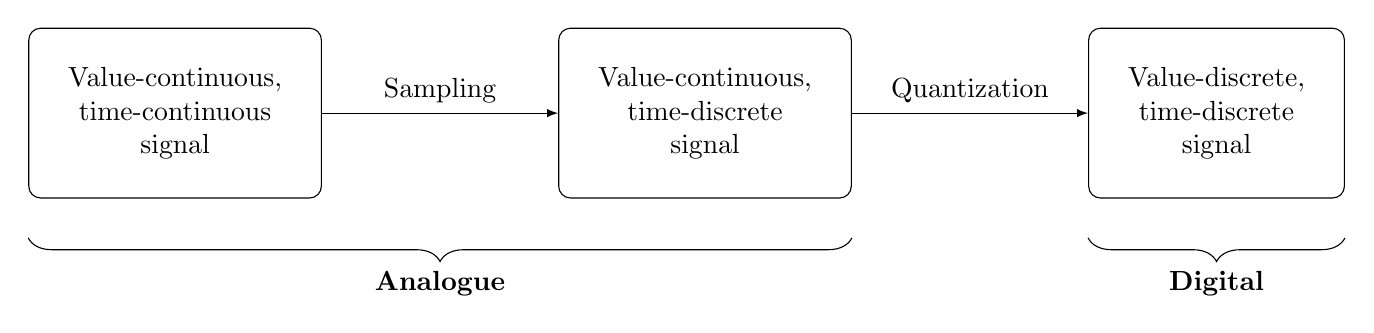
\begin{tikzpicture}
			\draw node[draw, block](Continuous){Value-continuous,\\ time-continuous\\ signal};
			\draw node[draw, block, right=3cm of Continuous](Sampled){Value-continuous,\\ time-discrete\\ signal};
			\draw node[draw, block, right=3cm of Sampled](Digital){Value-discrete,\\ time-discrete\\ signal};
			
			\draw [-latex] (Continuous) -- node[midway, align=center, above]{Sampling} (Sampled);
			\draw [-latex] (Sampled) -- node[midway, align=center, above]{Quantization} (Digital);
			
			\draw[decorate, decoration={brace, amplitude=3mm, mirror}] ([yshift=-5mm] Continuous.south west) -- ([yshift=-5mm] Sampled.south east) node[midway, below, yshift=-3mm]{\textbf{Analogue}};
			\draw[decorate, decoration={brace, amplitude=3mm, mirror}] ([yshift=-5mm] Digital.south west) -- ([yshift=-5mm] Digital.south east) node[midway, below, yshift=-3mm]{\textbf{Digital}};
		\end{tikzpicture}
	\end{adjustbox}
	\caption{Conversion from analogue to digital signals}
	\label{fig:ch01:signals_sampling}
\end{figure}

\begin{figure}[H]
	\centering
	%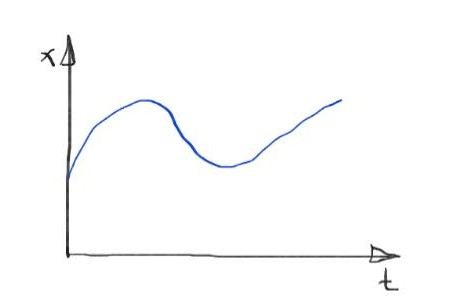
\includegraphics{../chapter01/Signal_Analogue.jpg}
	\begin{tikzpicture}
		\begin{axis}[
			height={0.25\textheight},
			width=0.6\linewidth,
			scale only axis,
			xlabel={$t$},
			ylabel={$x$},
			%grid style={line width=.6pt, color=lightgray},
			%grid=both,
			grid=none,
			axis lines=left,
			legend pos=north east,
			xmin=0,
			xmax=7,
			ymin=0,
			ymax=3,
			xtick={0, 1, ..., 6},
			ytick={0, 0.5, ..., 2.5}
		]
			\addplot[smooth, blue, thick] coordinates {(0, 1.1) (1, 1.8) (2, 2.1) (3, 1.0) (4, 0.8) (5, 1.7) (6, 2.4)};
		\end{axis}
	\end{tikzpicture}
	\caption[An analogue, value-continuous, time-continuous signal]{An analogue, value-continuous, time-continuous signal. Both time and value can be any real number.}
	\label{fig:ch01:Signal_Analogue}
\end{figure}

\begin{figure}[H]
	\centering
	%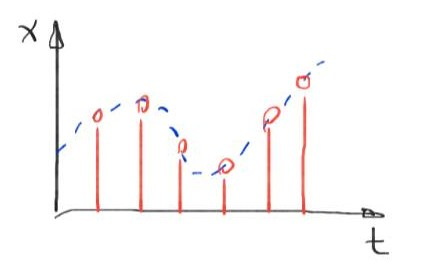
\includegraphics{../chapter01/Signal_TimeDiscr.jpg}
	\begin{tikzpicture}
		\begin{axis}[
			height={0.25\textheight},
			width=0.6\linewidth,
			scale only axis,
			xlabel={$t$},
			ylabel={$x$},
			%grid style={line width=.6pt, color=lightgray},
			%grid=both,
			grid=none,
			axis lines=left,
			legend pos=north east,
			xmin=0,
			xmax=7,
			ymin=0,
			ymax=3,
			xtick={0, 1, ..., 6},
			ytick={0, 0.5, ..., 2.5}
		]
			\addplot[smooth, blue, dashed] coordinates {(0, 1.1) (1, 1.8) (2, 2.1) (3, 1.0) (4, 0.8) (5, 1.7) (6, 2.4)};
			\addplot[red, thick] coordinates {(0, 0) (0, 1.1)};
			\addplot[red, thick] coordinates {(1, 0) (1, 1.8)};
			\addplot[red, thick] coordinates {(2, 0) (2, 2.1)};
			\addplot[red, thick] coordinates {(3, 0) (3, 1.0)};
			\addplot[red, thick] coordinates {(4, 0) (4, 0.8)};
			\addplot[red, thick] coordinates {(5, 0) (5, 1.7)};
			\addplot[red, thick] coordinates {(6, 0) (6, 2.4)};
			\addplot[only marks, red, thick, mark=o] coordinates {(0, 1.1) (1, 1.8) (2, 2.1) (3, 1.0) (4, 0.8) (5, 1.7) (6, 2.4)};
		\end{axis}
	\end{tikzpicture}
	\caption[An analogue, value-continuous, but time-discrete signal]{An analogue, value-continuous, but time-discrete signal. Only certain time points (in this case $t \in \mathbb{Z}$) are valid, but the values can be any real number. The red circles form the signal. The vertical lines illustrate that the signal in time-discrete. The blue, dashed signal is not present, but illustrates the original time-continuous signal from which the time-discrete signal has been obtained.}
	\label{fig:ch01:Signal_TimeDiscr}
\end{figure}

\paragraph{Digital signals.}

\index{signal!digital signal}
\index{signal!value-discrete}
Digital signals are both time-discrete and value-discrete. \emph{Value-discrete} means that they can take only one state out of a limited set of states.

\begin{figure}[H]
	\centering
	%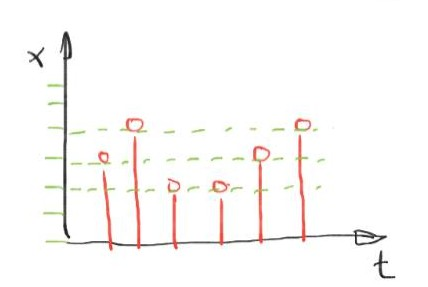
\includegraphics{../chapter01/Signal_Digital.jpg}
	\begin{tikzpicture}
		\begin{axis}[
			height={0.25\textheight},
			width=0.6\linewidth,
			scale only axis,
			xlabel={$t$},
			ylabel={$x$},
			%grid style={line width=.6pt, color=lightgray},
			%grid=both,
			xmajorgrids=false,
			ymajorgrids=true,
			grid style={color=lightgray, dashed},
			axis lines=left,
			legend pos=north east,
			xmin=0,
			xmax=7,
			ymin=0,
			ymax=3,
			xtick={0, 1, ..., 6},
			ytick={0, 0.5, ..., 2.5}
		]
			\addplot[smooth, blue, dashed] coordinates {(0, 1.1) (1, 1.8) (2, 2.1) (3, 1.0) (4, 0.8) (5, 1.7) (6, 2.4)};
			\addplot[red, thick] coordinates {(0, 0) (0, 1.0)};
			\addplot[red, thick] coordinates {(1, 0) (1, 2.0)};
			\addplot[red, thick] coordinates {(2, 0) (2, 2.0)};
			\addplot[red, thick] coordinates {(3, 0) (3, 1.0)};
			\addplot[red, thick] coordinates {(4, 0) (4, 1.0)};
			\addplot[red, thick] coordinates {(5, 0) (5, 1.5)};
			\addplot[red, thick] coordinates {(6, 0) (6, 2.5)};
			\addplot[only marks, red, thick, mark=o] coordinates {(0, 1.0) (1, 2.0) (2, 2.0) (3, 1.0) (4, 1.0) (5, 1.5) (6, 2.5)};
		\end{axis}
	\end{tikzpicture}
	\caption[A digital, value-discrete, time-discrete signal]{A digital, value-discrete, time-discrete signal. Only certain time points and a limited set of values (in this case multiples of $0.5$) are valid.}
	\label{fig:ch01:Signal_Digital}
\end{figure}

Examples:
\begin{itemize}
	\item Text letters
	\item Morse code
	\item Coded data
\end{itemize}

\index{signal!binary signal}
A special kind of digital signal is the \textbf{binary signal}. It has two discrete states.

\begin{excursus}{How analogue are digital signals?}
	In fact, the physical form of a digital signal is again an analogue signal. If digital electronics are implemented, digital signals are transferred into a physical form. A binary signal can take the discrete states ``high'' and ``low''. Being on a wire, its states are represented by voltage levels, for example \SI{0}{V} and \SI{3.3}{V}. At this point, the engineer must carefully consider the effects which the signal is subject to. This topic is covered by the field of microwave engineering and \ac{EMC}.
	
	However, if processed by a digital system, the physical representation is of minor importance. The theoretical consideration of digital signals neglects the physical nature. Even more, it is irrelevant which physical form of the digital signal exists and whether it exits. Only the discrete, logical states are of interest.
\end{excursus}


\subsection{Transmission Channels}

\index{transmission channel}
Digital communication systems employ electromagnetic waves to convey information. Therefore, only transmission channels transporting electromagnetic waves are considered.

\begin{figure}[H]
	\centering
	\begin{tikzpicture}
	\draw node[block](Main){\textbf{Transmission}\\ \textbf{channels}};
	\draw node[block, below left=of Main](Wired){Wired\\ channels};
	\draw node[block, below right=of Main](Wireless){Wireless\\ channels};
	
	\draw [-latex] (Main) -- (Wired);
	\draw [-latex] (Main) -- (Wireless);
	\end{tikzpicture}
	\caption{Classification of transmission channels}
	\label{fig:ch01:trans_ch_classif}
\end{figure}

\paragraph{Wired Channels.}

The electromagnetic wave propagates along a transmission line.

Examples of transmission lines:
\begin{itemize}
	\item Cables
	\begin{itemize}
		\item Two wire, twisted-pair \index{twisted-pair cable}
		\item Coaxial cable \index{coaxial cable}
	\end{itemize}
	\item Waveguides \index{waveguide}
	\item Planar lines (on printed circuit boards or integrated circuits)
	\begin{itemize}
		\item Microstrip \index{microstrip}
		\item Coplanar waveguide \index{coplanar waveguide}
	\end{itemize}
	\item Glass fibre (light is an electromagnetic wave, too)
\end{itemize}

\paragraph{Wireless Channels.}

The electromagnetic wave is not bound to a transmission line. It propagates through the space. A medium is not necessary. Electromagnetic wave can also travel through vacuum.

\section{The Electromagnetic Spectrum}

The carrier of information in an electronic communication system are electromagnetic waves -- either bound to a transmission line or wireless. Electromagnetic waves are electric fields $\underline{E}$ and magnetic fields $\underline{H}$, which oscillate at high frequencies.

\begin{excursus}{Maxwell's equations and wave equations}
	The Maxwell's equations are a set of coupled partial differential equations. They are the foundation of classical electromagnetism and classical optics.
	
	\textbf{Gauss' law:}
	\begin{equation}
		\nabla \cdot \cmplxvect{E} = \frac{\rho}{\varepsilon_0}
	\end{equation}
	
	\textbf{Gauss' law of magnetism:}
	\begin{equation}
		\nabla \cdot \cmplxvect{B} = 0
	\end{equation}
	
	\textbf{Faraday's law (electromagnetic induction):}
	\begin{equation}
		\nabla \times \cmplxvect{E} = - \frac{\partial \cmplxvect{B}}{\partial t}
	\end{equation}
	
	\textbf{Ampere's circuital law with Maxwell's extension:}
	\begin{equation}
		\nabla \times \cmplxvect{B} = \mu_0 \left(\cmplxvect{J} + \varepsilon_0 \frac{\partial \cmplxvect{E}}{\partial t} \right)
	\end{equation}
	
	James Clerk Maxwell postulated electromagnetic waves in 1865 \cite{Maxwell1864}. By ``decoupling'' the Maxwell's equations, the wave equations can be isolated for both the electric field and the magnetic field. They describe the wave propagation in any media.
	\begin{subequations}
		\begin{align}
			\Delta \cmplxvect{E} - \underline{\gamma}^2 \cmplxvect{E} &= \vect{0} \\
			\Delta \cmplxvect{H} - \underline{\gamma}^2 \cmplxvect{H} &= \vect{0}
		\end{align}
	\end{subequations}
	where $\underline{\gamma}$ is the complex propagation constant, that devolves into the attenuation constant $\alpha$ and the phase constant $\beta$. $\alpha$ expresses the decrease of the field amplitudes while the wave travels through a lossy medium. $\beta$ determines the propagation speed and the wavelength $\lambda = 2 \pi / \beta$.
	\begin{equation}
		\underline{\gamma} = \alpha + \mathsf{j} \beta
	\end{equation}
\end{excursus}

\begin{figure}[H]
	\centering
	\includegraphics[width=0.8\linewidth]{svg/ch01_EM_Spectrum_Properties.pdf}
	\caption{Diagram of the electromagnetic spectrum. \licensequote{\cite{Inductiveload2007}}{''Inductiveload''}{\href{https://creativecommons.org/licenses/by-sa/3.0/deed.en}{CC-BY-SA 3.0}}}
\end{figure}

Electromagnetic waves have different properties and applications, depending on the frequency. The most interesting range for communication is from radio waves to visible light.
\begin{itemize}
	\item Infrared and visible light are used in glass fibre (optical) communication systems. Before the appearance of electronic communication, light was an important information carrier (lighthouses, optical telegraphs, etc.).
	\item Radio waves and microwaves can be generated by electronics and are radiated by antennas. They have advantages over light like a wider range or their ability to penetrate walls.
\end{itemize}

Instead of the frequency, the \index{wavelength} \textbf{wavelength} $\lambda$ can be given. It is inverse proportional to the frequency with the proportionality constant $c_0$, the speed of light. The wavelength is the distance in which one period of the oscillating electromagnetic wave fits. The higher the frequency, the short the distance which a wave travels until the next period starts.
\begin{equation}
	\lambda = \frac{c_0}{f} = \frac{2 \pi c_0}{\omega}
\end{equation}

\begin{figure}[H]
	\centering
	\includegraphics[width=0.5\linewidth]{svg/ch01_Electromagnetic-Spectrum.pdf}
	\caption{Zooming into the radio spectrum as apart of the electromagnetic spectrum. \licensequote{\cite{Penubag2012}}{"Penubag" and Victor Blacus}{\href{https://creativecommons.org/licenses/by-sa/3.0/deed.en}{CC-BY-SA 3.0}}}
\end{figure}

Radio waves are used as a information carrier since the beginning of the 20th century. They can be further divided in accordance with their properties. The radio spectrum is split into \index{band} \textbf{bands}.

\renewcommand{\arraystretch}{1.5}
\begin{table}[H]
	\centering
	\caption[ITU radio band plan]{\ac{ITU} radio band plan}
	\begin{tabular}{|l|l|l|l|}
		\hline
		Band & Frequency & Properties & Example Applications \\
		\hline
		\hline
		\acs{ELF} & \SIrange{3}{30}{Hz} & \multirow{3}{*}{\begin{minipage}{0.25\textwidth}can penetrate water,\\ follows earth curvature\end{minipage}} & \multirow{3}{*}{\begin{minipage}{0.25\textwidth}submarine communication\end{minipage}} \\
		\cline{1-2}
		\acs{SLF} & \SIrange{30}{300}{Hz} &  &  \\
		\cline{1-2}
		\acs{ULF} & \SIrange{300}{3000}{Hz} &  &  \\
		\cline{1-4}
		\acs{VLF} & \SIrange{3}{30}{kHz} & \multirow{3}{*}{\begin{minipage}{0.25\textwidth}follows earth curvature\end{minipage}} & \begin{minipage}{0.25\textwidth}time signals, geophysics\end{minipage} \\[1.5em]
		\cline{1-2}
		\cline{4-4}
		\acs{LF} & \SIrange{30}{300}{kHz} &  & \begin{minipage}{0.25\textwidth}time signals, maritime navigation, AM broadcasting\end{minipage} \\[1.5em]
		\cline{1-2}
		\cline{4-4}
		\acs{MF} & \SIrange{300}{3000}{kHz} &  & \begin{minipage}{0.25\textwidth}AM broadcasting, aviation navigation, avalanche beacon\end{minipage} \\[1.5em]
		\cline{1-4}
		\acs{HF} & \SIrange{3}{30}{MHz} & \begin{minipage}{0.25\textwidth}reflections at ionosphere\end{minipage} & \begin{minipage}{0.25\textwidth}AM broadcasting, amateur radio, \acs{RFID}, maritime communication, long-distance aviation communication\end{minipage} \\[1.5em]
		\cline{1-4}
		\acs{VHF} & \SIrange{30}{300}{MHz} & \begin{minipage}{0.25\textwidth}quasi-optical propagation,\\ reflections at ionosphere possible\end{minipage} & \begin{minipage}{0.25\textwidth}FM broadcasting, television broadcasting, maritime and aviation communication, land mobile communication, weather satellites\end{minipage} \\[1.5em]
		\cline{1-4}
		\acs{UHF} & \SIrange{300}{3000}{MHz} & \multirow{3}{*}{\begin{minipage}{0.25\textwidth}quasi-optical propagation,\\ higher frequencies generally mean higher attenuation and shorter ranges\end{minipage}} & \begin{minipage}{0.25\textwidth}television broadcasting, \acs{WLAN}, \acs{GPS}, communication satellites, cell phones\end{minipage} \\[1.5em]
		\cline{1-2}
		\cline{4-4}
		\acs{SHF} & \SIrange{3}{30}{GHz} &  & \begin{minipage}{0.25\textwidth}radio astronomy, communication satellites, radar, satellite television broadcasting\end{minipage} \\[1.5em]
		\cline{1-2}
		\cline{4-4}
		\acs{EHF} & \SIrange{30}{300}{GHz} &  & \begin{minipage}{0.25\textwidth}new \acs{WLAN} standard (IEEE\,802.11ad), radar, radio astronomy, imaging (millimeter wave scanners), remote sensing\end{minipage} \\[1.5em]
		\hline
	\end{tabular}
\end{table}

Especially, the bands LF to UHF have been traditionally used in wireless communication. Furthermore, their usage is not limited to wireless systems. For example, cable television uses parts of the VHF or UHF spectra. Cable internet shares the wire with TV broadcasting.

Because of the increasing number of services and growing demands regarding bandwidth and response time, modern communication system advance in the direction of microwaves. The microwave spectrum begins at \SI{3}{GHz}.
%There are dedicate band plans for microwave applications. Table \ref{tab:ch01:IEEE_radar_bands} IEEE radar bands.

%\begin{table}[H]
%	\centering
%	\caption{IEEE radar bands}
%	\label{tab:ch01:IEEE_radar_bands}
%	\begin{tabular}{|l|}
%		\hline
%		Abbreviation \\
%		\hline
%		\hline
%		HF \\
%		\hline
%	\end{tabular}
%\end{table}

The services using the electromagnetic spectrum receive a \index{frequency allocation} \textbf{frequency allocation}. Usually, a national telecommunication regulation authority is responsible for allocation frequencies to the services. They follow recommendations of the \ac{ITU}, a special agency of the \ac{UN}. In Germany, the regulation authority is the Federal Network Agency (Bundesnetzagentur).

\section{Computer Networks}


This course focuses on the technologies which convey information between endpoints, using electromagnetic waves. The information, being conveyed, are called \textbf{data}. The handling of the data is a subject of computer science, especially \emph{computer networks} \index{computer network}. Since data processing is a part of digital communication systems, too, this digression shall give an overview about the employed concepts.


\subsection{Protocols}

Modern communication systems convey information world-wide. These communication links are established over myriads of devices, which form a network. The biggest computer network is the internet.

In order to interact, the devices are required to follow certain rules, which are called \textbf{communication protocols} \index{communication protocol}. Protocols define
\begin{itemize}
	\item the structure and semantics of data,
	\item synchronization of communication, and
	\item possible error recovery methods.
\end{itemize}

Protocols are standardized and must be implemented in every device, which interacts with other devices. Important standardization organizations are amongst others:
\begin{itemize}
	\item The non-profit organization \textbf{\acf{IETF}} issues standards concerning the internet. The standards are called \emph{Request For Comment} (RFC) and are available for everyone for free. Example standards: \ac{IP}, \ac{HTTP}
	\item The \textbf{\acf{IEEE}} has standards committees which develop and publish standards. With respect to the internet, the IEEE\,802 LAN/MAN Standards Committee is the most important one. Example standards: IEEE\,802.11 (\ac{WLAN}, Wifi)
	\item The \textbf{\acf{ETSI}} is an independent, non-profit standardization organization. It is recognized by the European Council and officially responsible for standardization of information and communication technologies in Europe. Example standards: 3G (cell phone system), 4G (cell phone system), TETRA (professional mobile radio system)
\end{itemize}


\subsection{\acs{OSI} Model}

There are many task which a digital communication systems must accomplish.
\begin{itemize}
	\item An application processes user input and displays data to the user.
	\item The application data must be reliably transferred over a network with many nodes.
	\item The network is shared with other users and applications.
	\item The network consists of many links using different physical transmission channels, for example, wired and wireless.
\end{itemize}
For each task, there are communication protocols to solve it. Communication protocols are grouped by the task which they fulfil. There is an increasing level of abstraction from the physical link to the application data. The \index{OSI model} \textbf{\acs{OSI} Model} (Figure \ref{fig:ch01:osi_model}) defines a layer structure for classifying communication protocols, which regards the level of abstraction.

\begin{figure}[H]
	\centering
	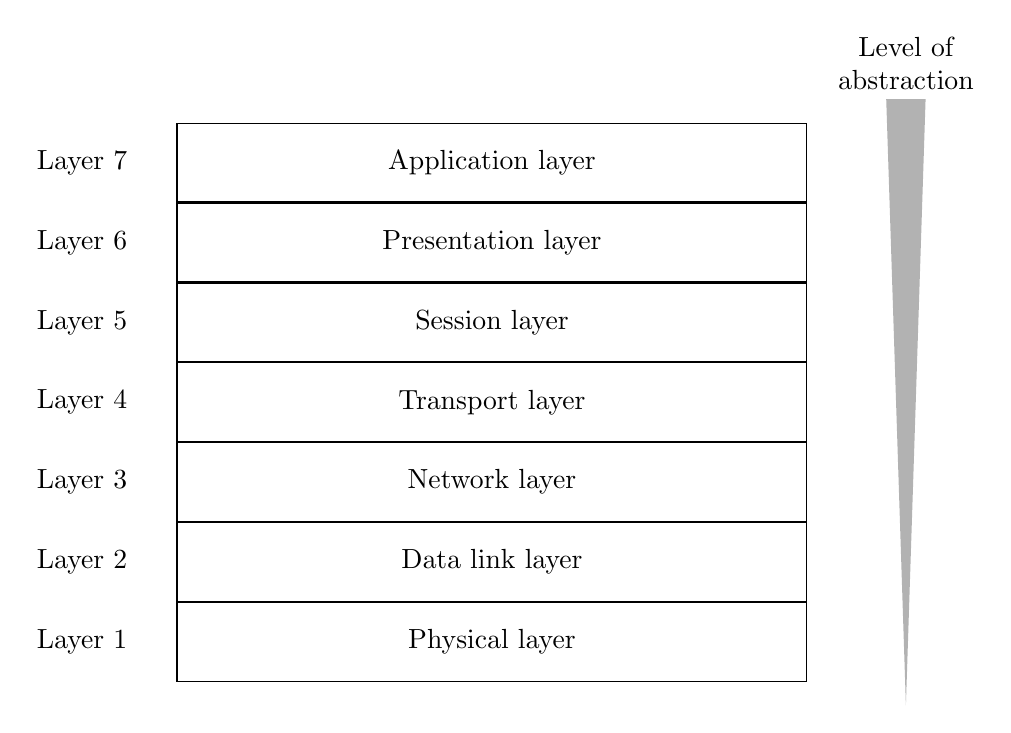
\begin{tikzpicture}[
		layer/.style={
			rectangle,
			minimum height=1cm,
			minimum width=8cm
		}
	]
		\draw node[draw, layer](L7){Application layer};
		\draw node[draw, layer, below=0 of L7](L6){Presentation layer};
		\draw node[draw, layer, below=0 of L6](L5){Session layer};
		\draw node[draw, layer, below=0 of L5](L4){Transport layer};
		\draw node[draw, layer, below=0 of L4](L3){Network layer};
		\draw node[draw, layer, below=0 of L3](L2){Data link layer};
		\draw node[draw, layer, below=0 of L2](L1){Physical layer};
		
		\node [anchor=east, align=right] at([xshift=-5mm] L7.west) {Layer 7};
		\node [anchor=east, align=right] at([xshift=-5mm] L6.west) {Layer 6};
		\node [anchor=east, align=right] at([xshift=-5mm] L5.west) {Layer 5};
		\node [anchor=east, align=right] at([xshift=-5mm] L4.west) {Layer 4};
		\node [anchor=east, align=right] at([xshift=-5mm] L3.west) {Layer 3};
		\node [anchor=east, align=right] at([xshift=-5mm] L2.west) {Layer 2};
		\node [anchor=east, align=right] at([xshift=-5mm] L1.west) {Layer 1};
		
		\filldraw[fill=gray!60, draw=none] ([xshift=10mm, yshift=3mm] L7.north east) -- node[midway, above, anchor=south, align=center]{Level of\\ abstraction} ([xshift=15mm, yshift=3mm] L7.north east) -- ([xshift=12.5mm, yshift=-3mm] L1.south east);
	\end{tikzpicture}
	\caption[OSI Model with seven layers]{\ac{OSI} Model with seven layers}
	\label{fig:ch01:osi_model}
\end{figure}

\begin{table}[H]
	\caption[Description of the layers of the OSI Model]{Description of the layers of the \ac{OSI} Model (Figure \ref{fig:ch01:osi_model}). The protocol data unit is the information }
	\begin{tabular}{|l|l|p{0.5\linewidth}|}
		\hline
		Layer & PDU & Function \\
		\hline
		\hline
		7: Application & Data & Processing user inputs, displaying data, providing services \\
		\hline
		6: Presentation & Data & Translation between network service and application (encryption, compression, etc.) \\
		\hline
		5: Session & Data & Managing sessions (retaining the communication state across multiple contacts) \\
		\hline
		4: Transport & Datagram, Segment & Reliable communication (segmentation, multiplexing, data loss detection) \\
		\hline
		3: Network & Packet & Data transfer across multiple nodes (addressing, routing, traffic control) \\
		\hline
		2: Data link & Frame & Transmission between two devices (medium access, flow control) \\
		\hline
		1: Physical & Symbol & Transmission over a physical medium \\
		\hline
	\end{tabular}
\end{table}

Each protocol has a standardized interface exposed to the upper layer, called \index{service access point} \textbf{\ac{SAP}}. They allow an upper layer protocol to execute functions of the lower layer protocol. These functions are, for example:
\begin{itemize}
	\item Sending or receiving data
	\item Control operations
	\item Network registration and de-registration
\end{itemize}

Protocol layers add own information to the data received from the upper layer. This additional information is required to provide the protocol's functionality. For example, the \acf{IP} needs to add the source and destination address, so that the packet can be routed to the correct endpoint. One can imagine this like data which is written on a letter, which is put into an envelope, which itself is put into another envelope, and so on.

\begin{figure}[H]
	\centering
	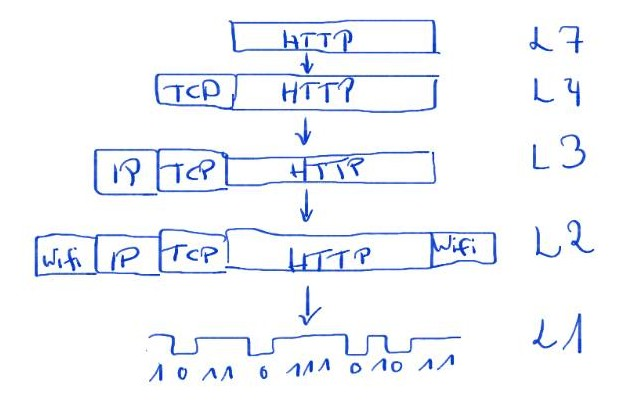
\includegraphics{../chapter01/Frame_Wrapping.jpg}
	\caption{Principle of adding more information in each protocol layer}
	\label{fig:ch01:frame_construction}
\end{figure}

Communication protocols may be exchanged in one layer without affecting the functionality of the other layers. For example, \ac{HTTP} operates on \acs{TCP}/\acs{IP}. But the \acf{IP} works on multiple physical links like Ethernet (IEEE\,802.3), Wifi (IEEE\,802.11) or 4G. The transmission media can even change along the communication path. Information travelling through the internet experience lots of \index{media change} \textbf{media changes}. For example, a datagram is firstly sent over a \ac{WLAN} link an relayed by the router on a cable to the internet service provider.


%\begin{figure}[H]
%	\centering
%	\caption{Media change on the internet. }
%	\label{fig:ch01:media_changes}
%\end{figure}

This course on digital communication systems mainly considers the physical layer (layer 1) and the data link layer (layer 2). This physical layer converts the information to physical signals which then leave the device to be transmitted over a physical transmission channel. Networks, which are enabled by protocols of layer 3 and above, are outside the scope of this course.


\subsection{Network Topologies}

In the context of networks,
\begin{itemize}
	\item the devices are called \index{node} \textbf{nodes} and
	\item the communication channels between the nodes are called \index{link} \textbf{links}.
\end{itemize}

Nodes of a network can be arranged in various ways. The structures being formed are \index{network topology} \textbf{network topologies}. Basic topologies are:
\begin{itemize}
	\item \textbf{Line} or chain -- The nodes are connected in series. A packet is passed on by each node until reaches its destination.
	\item \textbf{Ring} -- An extension of the line where the outer nodes are interconnected, too. A packet is passed by every node to its destination. The failure of a single node does not split the network into two segments, which increases the fault tolerance.
	\item \textbf{Bus} -- All nodes are connected to a central cable, the bus. Each node can receive the signals transmitted. As a drawback, only one device may occupy the bus simultaneously for transmission.
	\item \textbf{Star} -- A central node (a hub or switch) relays the packets to its destination.
	\item \textbf{Tree} -- Tree structure is a hybrid network of star networks interconnected by a bus. Because there a no loops in the network, the nodes can be graphically re-ordered to a tree graph.
	\item \textbf{Mesh} -- The nodes are interconnected directly. Nodes may have many direct connections to other nodes, while there is no hierarchy. There are many loops in the network. Usually, mesh networks are re-organized dynamically in mobile systems. A node discovers all nodes which it can reach and establishes a link. A special form is the \emph{Full Mesh}, where all nodes are interconnected with every other one.
\end{itemize}

\begin{figure}[H]
	\centering
	\includegraphics[width=0.7\linewidth]{svg/ch01_NetworkTopologies.pdf}
	\caption{Network topologies. \licensequote{\cite{Maksim2011}}{``Maksim'' and ``Malyszkz''}{Public Domain}}
\end{figure}

The network topology is a concern of the physical and data link layers of the \ac{OSI} model. It can be physical or logical.
\begin{itemize}
	\item The \index{network topology!physical topology} \textbf{physical topology} refers to the placement of the hardware. For example, in a cable network, the physical topology is defined by the cables which interconnect the devices. The topology is mainly implemented in the physical layer.
	\item The \index{network topology!logical topology} \textbf{logical topology} models the data flow in the network. For example, in a wireless network, each node can receive the signals of all other nodes in range. By addressing the devices and filtering out packets with wrong destination addresses, a logical network is created on top of the physical wireless interface. The topology is mainly implemented in the data link layer.
\end{itemize}

A network must fulfil requirements, which determine the network topology, in the end. The use case and constraints must be considered by the engineer. For example:
\begin{itemize}
	\item Lines and trees lack in reliability. The failure of one node divides the network into two segments and the remaining nodes cannot communicate with each other.
	\item The ring is an improvement of the line with respect to reliability. Lines and rings require that all nodes have equal power. Otherwise, the weakest node would be a bottleneck with respect to network bandwidth.
	\item Mesh and fully connected topologies are fault tolerant. The failure of one node does not corrupt the whole network. Furthermore, high data rates and lower latencies may be reached due to a higher number of links.
	\item Mesh and fully connected topologies increase the cost of the networks. Each link consumes energy, space and money.
	\item Buses and stars reduce the cost by maintaining a reasonable amount of reliability. The failure of one device has no major impact on the network, but a disturbance of the bus may. Buses can only be occupied by one node simultaneously. The results in lower data rate and higher latency compared to meshes.
\end{itemize}
An optimal topology may mix the basic forms.

\phantomsection
\addcontentsline{toc}{section}{References}
\printbibliography[heading=subbibliography]
\end{refsection}


\clearpage
\phantomsection
\addcontentsline{toc}{section}{Exercise 1}
\section*{Exercise 1}

\begin{question}
	What is the difference between a \emph{digital communication system} and a \emph{service}? To which OSI layers are they associated?
\end{question}
\clearpage

\chapter{Time-Continuous Signals and Systems}

\begin{refsection}

All signals considered in this chapter are \index{signal!deterministic signal} \textbf{deterministic}, i.e., its values are predictable at any time. Especially, the values can be calculated by a mathematical equation. In contrast, \emph{random} signals are not predictable. Its values are subject to a random process, which must be modelled stochastically.

\index{signal!time-continuous}
\begin{figure}[H]
	\centering
	\begin{tikzpicture}
		\draw node[block](Signals){\textbf{Signal}\\ \textbf{(deterministic)}};
		\draw node[block, below left=of Signals](Periodic){Periodic};
		\draw node[block, below right=of Signals](NonPeriodic){Non-periodic};
		\draw node[block, below left=of Periodic](Mono){Mono-chromatic};
		\draw node[block, below right=of Periodic](Multi){Multi-frequent};
		
		\draw [-latex] (Signals) -- (Periodic);
		\draw [-latex] (Signals) -- (NonPeriodic);
		\draw [-latex] (Periodic) -- (Mono);
		\draw [-latex] (Periodic) -- (Multi);
	\end{tikzpicture}
	\caption{Classification of time-continuous signals}
	\label{fig:ch02:timecont_signals_classif}
\end{figure}

\section{Mono-Chromatic Signals}

\paragraph{Representation by A Real-Valued Function.}

The mono-chromatic signal $x_{mc}(t)$ is defined by:
\begin{equation}
	x_{mc}(t) = \hat{X} \cdot \cos\left(\omega_0 t - \varphi_0\right)
	\label{eq:ch02:mono_chrom_eq}
\end{equation}
where

\begin{tabular}{ll}
	$\hat{X}$ & is the \index{amplitude} \textbf{amplitude} of the signal, \\
	$\omega_0$ & is the \index{angular frequency} \textbf{angular frequency} of the signal, \\
	$\varphi_0$ & is the \index{phase} \textbf{phase} of the signal, \\
	$t \in \mathbb{R}$ & is the real-value time variable and continuously defined.
\end{tabular}

In fact, the sine function $\sin()$ is mono-chromatic, too. However, it can be derived from \eqref{eq:ch02:mono_chrom_eq} with $\varphi_0 = \SI{90}{\degree}$.

\begin{equation*}
	x_{sin}(t) = \hat{X} \cdot \sin\left(\omega_0 t\right) = \cos\left(\omega_0 t - \SI{90}{\degree}\right)
\end{equation*}

The angular frequency is connected to the \index{frequency} \textbf{frequency}.
\begin{equation}
	\omega_0 = 2 \pi f_0
\end{equation}

\begin{attention}
	You must not confuse the terms \emph{frequency} and \emph{angular frequency}!
\end{attention}

The inverse of the frequency is the \index{period} \textbf{period} $T_0$. It is the time interval at which the signal repeats.
\begin{equation}
	T_0 = \frac{1}{f_0} = \frac{2 \pi}{\omega_0}
\end{equation}

Be aware of the units. The period $T_0$ is defined in seconds \si{s}. The frequency $f_0$ is the inverse of seconds, which is Hertz \si{Hz}. The angular frequency $\omega_0$ is the inverse of seconds, too. However, it is never given in Hertz, only in \si{rad/s} or, more commonly, \si{1/s}.

\begin{table}[H]
	\centering
	\caption{Units}
	\begin{tabular}{|l|l|}
		\hline
		Period $T_0$ & \si{s} \\
		\hline
		Frequency $f_0$ & \si{Hz} \\
		\hline
		Angular frequency $\omega_0$ & \si{1/s} \; (never Hertz!) \\
		\hline
	\end{tabular}
\end{table}

The actual unit of the signal is derived from its amplitude $\hat{X}$ which can be any physical measure.

\paragraph{Representation by A Complex-Valued Phasor.}

A graphical view on the creation of a cosine signal is depicted in Figure \ref{fig:ch02:cos_creation}.

\begin{figure}[H]
	\caption{Imagine, there is a pointer (red) with one side fixed to a point. Now, it begins rotating counter-clockwise with an angular frequency of $\omega_0$ (blue). The arrow of the pointer draws a circle (left side). Each angle of the pointer is related to a time instance (green). The blue pointer is the current position at time instance $t$. Its vertical value is projected into the time plot, forming the cosine wave (orange).}
	\label{fig:ch02:cos_creation}
\end{figure}

You may now some relations:
\begin{itemize}
	\item A full rotation of the pointer takes exactly one period $T_0$.
	\item The orange cosine curve can be horizontally shifted by redefining the original angle of the pointer at $T_0$. This offset angle is the phase $\varphi_0$.
	\item The length of the pointer and the radius of the circle is the amplitude $\hat{X}$.
\end{itemize}

A mono-chromatic signal can be described by its three parameters
\begin{itemize}
	\item Amplitude $\hat{X}$
	\item Phase $\varphi_0$
	\item Frequency $\omega_0$
\end{itemize}

When a signal passes through a \ac{LTI} system, the amplitude, the phase or both may change. However, the frequency never changes. Thus, the frequency $\omega_0$ is assumed to be constant and neglected. Consequently, the parameters
\begin{itemize}
	\item amplitude $\hat{X}$ and
	\item phase $\varphi_0$
\end{itemize}
remain. Both are absorbed by the complex-valued \index{phasor} \textbf{phasor} $\underline{X}$, which uniquely describes a mono-chromatic signal.
\begin{equation}
	\underline{X} = \hat{X} \cdot e^{-j \varphi_0} = \hat{X} \angle -\varphi_0
\end{equation}

\begin{excursus}{Complex numbers}
	$j$ is the \index{imaginary unit} \textbf{imaginary unit}. It satisfies the equation
	\begin{equation}
		j^2 = -1
	\end{equation}
	There is no real number $j \notin \mathbb{R}$ which satisfies the above solution. $j$ spans the set of complex numbers $\mathbb{C}$.
	
	In mathematics, the imaginary unit is noted as $i$. In engineering context, $j$ is used instead, because $i$ is the symbol of the electric current.
	
	A complex number $\underline{c} \in \mathbb{C}$ can be noted in \index{cartesian form} \textbf{cartesian form}:
	\begin{equation}
		\underline{c} = a + j b
	\end{equation}
	$a \in \mathbb{R}$ is the \index{real part} \textbf{real part} of $\underline{c}$. $b \in \mathbb{R}$ is the \index{imaginary part} \textbf{imaginary part} $\underline{c}$.
	\begin{subequations}
		\begin{align}
			a &= \Re\{\underline{c}\} \\
			b &= \Im\{\underline{c}\}
		\end{align}
	\end{subequations}
	Complex numbers $\underline{c}$ always carry an underline in this lecture to distinguish them from real numbers. However, this is not mandatory.

	Another notation is the \index{polar form} \textbf{polar form}:
	\begin{equation}
		\underline{c} = r \cdot e^{j \varphi}
	\end{equation}
	with
	\begin{subequations}
		\begin{align}
			r &= |\underline{c}| = \sqrt{\Re\{\underline{c}\}^2 + \Im\{\underline{c}\}^2} \\
			\varphi &= \mathrm{atan2} \left(\Im\{\underline{c}\}, \Re\{\underline{c}\}\right) \\
			e^{j \varphi} &= \cos \varphi + j \sin \varphi
		\end{align}
	\end{subequations}
	The polar form can be written in \index{angle notation} \textbf{angle notation}:
	\begin{equation}
		\underline{c} = r \angle \varphi
	\end{equation}
	$r \in \mathbb{R}$ and $\varphi \in \mathbb{R}$ are the \index{polar coordinates} \textbf{polar coordinates}.
\end{excursus}

The phasor $\underline{X} \in \mathbb{C}$ is a complex number, which is mostly represented in polar coordinates (see Figure \ref{fig:ch02:cmplxplane_phasor}).

\begin{figure}[H]
	\centering
	\begin{tikzpicture}
	\draw[->] (-3.2,0) -- (3.2,0) node[below, align=left]{$\Re$};
	\draw[->] (0,-3.2) -- (0,3.2) node[left, align=right]{$\Im$};
	\draw[->, thick] (0, 0) -- (-40:3) node[right, align=left]{Complex phasor $\underline{X}$\\ (position at $t = 0$)};
	\draw (0:1.5) arc(0:-40:1.5) node[midway, right, align=left]{Phase $\varphi_0$};
	
	\draw[->, dashed] (-50:1) arc(-50:30:1) node[right, align=left]{$\omega_0$};
	\end{tikzpicture}
	\caption{Phasor in the complex plane}
	\label{fig:ch02:cmplxplane_phasor}
\end{figure}

Figure \ref{fig:ch02:cmplxplane_phasor} depicts the phasor in the complex plane. Figure \ref{fig:ch02:cos_creation} shows a complex plane, too. Please note that both complex planes are rotated by \SI{90}{\degree} with respect to each other.

\begin{fact}
	The phasor of a signal is a signal parameter, constant and \underline{not} time-dependent.
\end{fact}

The current position of the pointer $\underline{x}(t)$ in the complex plane is obtained by rotating it. It makes a full rotation each $T_0$ periods. Therefore, it rotates at an angular frequency of $\omega_0$. The rotation is a multiplication by $e^{j \omega t}$ in the complex plane. $\underline{x}(t) \in \mathbb{C}$ is a complex value, too.
\begin{equation}
	\underline{x_{mc}}(t) = \underline{X} \cdot e^{j \omega t} = \hat{X} \cdot e^{-j \varphi_0} \cdot e^{j \omega t}
\end{equation}

\todo{Proof}

The real-valued function can be obtained by extracting the real part of the complex-valued current value.
\begin{equation}
	x_{mc}(t) = \Re\left\{\underline{x_{mc}}(t)\right\}
\end{equation}

\section{Periodic Signals and Fourier Series}

Periodic signals $x_p(t)$ comprises a class of signals which indefinitely repeat at constant time intervals $T_0$.
\begin{equation}
	x_p(t + n T_0) = x_p(t) \qquad \forall \; n \in \mathbb{Z}, \quad \mathbb{Z} = \left\{..., -2, -1, 0, 1, 2, ...\right\}
\end{equation}

Mono-chromatic signals are a special kind of periodic signals. Multi-frequent signals are composed a limited or unlimited number of mono-chromatic signals, which superimpose. Multi-frequent signals are periodic signals in general.

\begin{fact}
	Each periodic signal can be decomposed into a superposition of mono-chromatic signals.
\end{fact}

The inverse of the period $T_0$ is $f_0$, which is the \textbf{base frequency}. This is the frequency at the periodic pattern repeats. Again, frequency and angular frequency $\omega_0 = 2 \pi f_0$ must be distinguished.

The periodic signal can now be decomposed in cosine and sine functions with integer multiples of the base frequency $f_0$ or base angular frequency $\omega_0$, respectively. They are called \index{harmonics} \textbf{harmonics}.
\begin{equation}
	\begin{split}
		x_p(t) &= \sum\limits_{n=0}^{\infty} a_n \cos\left(n \omega_0 t\right) + \sum\limits_{m=0}^{\infty} b_m \sin\left(m \omega_0 t\right) \qquad \forall \; n, m \in \mathbb{N} = \left\{0, 1, 2, ...\right\} \\
		 &= a_0 + \sum\limits_{n=1}^{\infty} a_n \cos\left(n \omega_0 t\right) + \sum\limits_{m=1}^{\infty} b_m \sin\left(m \omega_0 t\right) \\
	\end{split}
	\label{eq:ch02:fourier_series}
\end{equation}

What happened to $n = 0$ and $m = 0$? $\cos(0) = 1$ and $\sin(0) = 0$. That's it.

Comparing to the mono-chromatic signals, what happened to the phase $\varphi_0$? The phase $\varphi_0$ is a characteristic of mono-chromatic signals. It is completely absorbed by the coefficients $a_n$ and $b_n$ of the cosine and sine functions.

\subsection{Orthogonality}
\index{orthogonality}
The cosine and sine functions are orthogonal to each other. In geometry, two vectors $\vect{A}$ and $\vect{B}$ are said to be orthogonal, if the angle between them is \SI{90}{\degree}. In this case, their inner product is zero.
\begin{equation}
	\langle \vect{A}, \vect{B} \rangle = 0
\end{equation}

More generally, two functions $f(x)$ and $g(x)$ are orthogonal if their \index{inner product} \textbf{inner product} $\langle f, g \rangle$ is zero. 
\begin{equation}
	0 \stackrel{!}{=} \langle f, g \rangle_w = \int\limits_{a}^{b} f(x) g(x) w(x) \, \mathrm{d} x
\end{equation}
$w(x)$ is a non-negative weight function, which is $w(x) = 1$ in simple cases like this one.

Now, you can prove that the cosine and sine functions are orthogonal to each other.
\begin{equation}
	\int\limits_{-\frac{T_0}{2}}^{\frac{T_0}{2}} \cos\left(n \omega_0 t\right) \sin\left(m \omega_0 t\right) \, \mathrm{d} t = 0 \qquad \forall \; n, m \in \mathbb{Z}
	\label{eq:ch02:orth_rel_cos_sin}
\end{equation}

Furthermore, the sine and cosine functions with \underline{different} indices are orthogonal to each other.
\begin{equation}
	\int\limits_{-\frac{T_0}{2}}^{\frac{T_0}{2}} \cos\left(n \omega_0 t\right) \cos\left(p \omega_0 t\right) \, \mathrm{d} t = \frac{\pi}{\omega_0} \cdot \delta_{np} \qquad \forall \; n, p \in \mathbb{N}
	\label{eq:ch02:orth_rel_cos}
\end{equation}
\begin{equation}
	\int\limits_{-\frac{T_0}{2}}^{\frac{T_0}{2}} \sin\left(m \omega_0 t\right) \sin\left(q \omega_0 t\right) \, \mathrm{d} t = \frac{\pi}{\omega_0} \cdot \delta_{mq} \qquad \forall \; m, q \in \mathbb{N}
	\label{eq:ch02:orth_rel_sin}
\end{equation}
with the Kronecker delta
\begin{equation}
	\delta_{uv} = \begin{cases}
		1 & \qquad \text{if } u = v, \\
		0 & \qquad \text{if } u \neq v
	\end{cases}
	\label{eq:ch02:kronecker_delta}
\end{equation}

The \index{orthogonality relations} \textbf{orthogonality relations} \eqref{eq:ch02:orth_rel_cos_sin}, \eqref{eq:ch02:orth_rel_cos} and \eqref{eq:ch02:orth_rel_sin} point out:
\begin{itemize}
	\item Cosine functions are orthogonal if their indices are different. I.e., $n \neq p$ in \eqref{eq:ch02:orth_rel_cos}.
	\item Sine functions are orthogonal if their indices are different. I.e., $m \neq q$ in \eqref{eq:ch02:orth_rel_sin}.
	\item Cosine and sine function are orthogonal independent of their indices.
	\item The indices are the integer multiples of the base frequency $\omega_0$ (harmonics).
\end{itemize}

\subsection{Extraction of The Coefficients}

The orthogonality relations are useful to extract the coefficients $a_n$ and $b_n$ in \eqref{eq:ch02:fourier_series}. Given is the input signal $\tilde{x}_p(t)$ whose coefficient shall be determined. Following assumptions can be derived from the properties of a periodic signal:
\begin{itemize}
	\item $\tilde{x}_p(t)$ is composed of mono-chromatic cosine and sine functions.
	\item All cosine and sine functions have integer multiples of the base frequency.
	\item Each cosine and sine function has a different weight -- the coefficient.
\end{itemize}

Using the orthogonality relations, the coefficients $\tilde{a}_n$ and $\tilde{b}_n$ can be obtained by:
\begin{subequations}
	\begin{align}
		\tilde{a}_n &= \frac{\omega_0}{\pi} \int\limits_{-\frac{T_0}{2}}^{\frac{T_0}{2}} \tilde{x}_p(t) \cdot \cos\left(n \omega_0 t\right) \, \mathrm{d} t \label{eq_ch02_fourier_series_coeff_an} \\
		\tilde{b}_m &= \frac{\omega_0}{\pi} \int\limits_{-\frac{T_0}{2}}^{\frac{T_0}{2}} \tilde{x}_p(t) \cdot \sin\left(n \omega_0 t\right) \, \mathrm{d} t \label{eq_ch02_fourier_series_coeff_bm}
	\end{align}
\end{subequations}

\begin{proof}{Parameter Extraction for $\tilde{a}_n$}
	Given is a periodic function $\tilde{x}_p(t)$, which can be decomposed into:
	\begin{equation}
		\tilde{x}_p(t) = \sum\limits_{p=0}^{\infty} \tilde{a}_p \cos\left(p \omega_0 t\right) + \sum\limits_{q=0}^{\infty} \tilde{b}_q \sin\left(q \omega_0 t\right)
		\label{eq_ch02_proof_per_sig_example}
	\end{equation}
	The coefficient $\tilde{a}_n$ is of interest.
	
	Inserting \eqref{eq_ch02_proof_per_sig_example} into \eqref{eq_ch02_fourier_series_coeff_an}, yields
	\begin{equation}
		\tilde{a}_n = \frac{\omega_0}{\pi} \int\limits_{-\frac{T_0}{2}}^{\frac{T_0}{2}} \left(\sum\limits_{p=0}^{\infty} \tilde{a}_p \cos\left(p \omega_0 t\right) + \sum\limits_{q=0}^{\infty} \tilde{b}_q \sin\left(q \omega_0 t\right)\right) \cdot \cos\left(n \omega_0 t\right) \, \mathrm{d} t
	\end{equation}
	Due to the orthogonality relations, \underline{all products containing a sine function} and \underline{all products containing a cosine function with the index $n \neq p$} become zero. Furthermore, following must be true: $n = p$
	
	\begin{equation}
		\tilde{a}_n = \tilde{a}_p \frac{\omega_0}{\pi} \int\limits_{-\frac{T_0}{2}}^{\frac{T_0}{2}} \cos\left(p \omega_0 t\right) \cdot \cos\left(n \omega_0 t\right) \, \mathrm{d} t \qquad \text{if } \; n = p
	\end{equation}
	
	Using \eqref{eq:ch02:orth_rel_cos}, the integral resolves to:
	\begin{equation}
		\tilde{a}_n = \tilde{a}_p \frac{\omega_0}{\pi} \frac{\pi}{\omega_0} \qquad \text{if } \; n = p
	\end{equation}
	
	In the end, it could be proven that $\tilde{a}_n = \tilde{a}_p$ for $n = p$.
	
	The proof is analogous for the coefficient $b_n$.
\end{proof}

$\cos\left(n \omega_0 t\right)$ can be seen as a ``test function'', which is used to extract the component with the index $n$. The proof points out:
\begin{itemize}
	\item All sine components are erased by $\cos\left(n \omega_0 t\right)$, due to the orthogonality relations.
	\item All cosine function with index $p \neq n$ are erased by $\cos\left(n \omega_0 t\right)$, due to the orthogonality relations.
\end{itemize}
For $b_m$, $\sin\left(m \omega_0 t\right)$ is analogous.

\begin{excursus}{Illustration of The ``Test Function''}
	For illustration of the ``test functions'', image you have a radio and want to hear a specific station. You tune to the frequency on which the station is broadcasting. All other signals are filtered out, you don't want to hear them. Actually, the radio does not employ orthogonality in this case. However, this illustration might help to understand the meaning of $\cos\left(n \omega_0 t\right)$ and $\sin\left(m \omega_0 t\right)$ \underline{in connection} with the orthogonality relations.
\end{excursus}

A special case is the coefficient $\tilde{a}_0$.
\begin{equation}
	\tilde{a}_0 = \frac{\omega_0}{\pi} \int\limits_{-\frac{T_0}{2}}^{\frac{T_0}{2}} \tilde{x}_p(t) \, \mathrm{d} t
\end{equation}
$\cos\left(n \omega_0 t\right)$ is $1$ for $n = 0$. $\tilde{a}_0$ is the \index{DC offset} \textbf{\ac{DC} offset} of the signal. The above formula is known as the calculation of the signal mean in electrical engineering.

\begin{definition}{Fourier series}
	The composition of a series of mono-chromatic signals as shown in \eqref{eq:ch02:fourier_series} is called \index{Fourier series} \textbf{Fourier series}.
	\begin{equation*}
		x_p(t) = \sum\limits_{n=1}^{\infty} a_n \cos\left(n \omega_0 t\right) + \sum\limits_{m=1}^{\infty} b_m \sin\left(m \omega_0 t\right)
	\end{equation*}
	
	The coefficients can be calculated using \eqref{eq_ch02_fourier_series_coeff_an} and \eqref{eq_ch02_fourier_series_coeff_bm}.
\end{definition}

\subsection{Complex-Valued Fourier Series}

A complex-valued, periodic signal $\underline{x_p}(t)$ can be decomposed into complex-valued mono-chromatic signals. The coefficients $\underline{c}_n$ are phasors.
\begin{equation}
	\underline{x_p}(t) = \sum\limits_{n = -\infty}^{\infty} \underline{c}_n \cdot e^{j n \omega_0 t} \qquad \forall \; n \in \mathbb{Z}
	\label{eq:ch02:fourier_series_cmplx}
\end{equation}

The coefficients $\underline{\tilde{c}}_n$ of an input signal $\underline{\tilde{x}_p}(t)$ can be determined by:
\begin{equation}
	\underline{\tilde{c}}_n = \frac{\omega_0}{2 \pi} \int\limits_{-\frac{T_0}{2}}^{\frac{T_0}{2}} \underline{\tilde{x}_p}(t) \cdot e^{-j n \omega_0 t} \, \mathrm{d} t
	\label{eq_ch02_fourier_series_coeff_cn}
\end{equation}

It is based on the orthogonality relation:
\begin{equation}
	\int\limits_{-\frac{T_0}{2}}^{\frac{T_0}{2}} e^{j n \omega_0 t} e^{-j p \omega_0 t} \, \mathrm{d} t = \frac{2 \pi}{\omega_0} \cdot \delta_{np} \qquad \forall \; n, p \in \mathbb{Z}
	\label{eq:ch02:orth_rel_exp}
\end{equation}

\begin{definition}{Complex-Valued Fourier series}
	A complex-valued, periodic signal $\underline{x_p}(t)$ can be decomposed into a series complex-valued mono-chromatic signals \eqref{eq:ch02:fourier_series_cmplx} -- the \index{Fourier series!complex-valued} \textbf{complex-valued Fourier series}.
	\begin{equation*}
		\underline{x_p}(t) = \sum\limits_{n = -\infty}^{\infty} \underline{c}_n \cdot e^{j n \omega_0 t} \qquad \forall \; n \in \mathbb{Z}
	\end{equation*}
	
	The coefficients can be calculated using \eqref{eq_ch02_fourier_series_coeff_cn}.
\end{definition}

\subsection{Amplitude and Phase Spectra}

Let's consider the complex-valued Fourier series $\underline{x_p}(t)$ \eqref{eq:ch02:fourier_series_cmplx}. The coefficients $\underline{c}_n$ are phasors. Its absolute value (amplitude) $|\underline{c}_n|$ and argument (phase) $\arg\left(\underline{c}_n\right)$ can now be plotted over the index $n$. The index $n \in \mathbb{Z}$ is discrete. Thus, the resulting plots are value-discrete in the dimension of $n$. In contrast, the amplitudes and phases are value-continuous.

\begin{definition}{Spectrum of a period signal}
	\begin{itemize}
		\item The plot of the amplitude $|\underline{c}_n|$ is called \index{amplitude spectrum} \textbf{amplitude spectrum}.
		\item The plot of the phase $\arg\left(\underline{c}_n\right)$ is called \index{phase spectrum} \textbf{phase spectrum}.
		\item When referring to the \index{spectrum} \textbf{spectrum}, generally both amplitude and phase, or their complex-valued representation of $\underline{c}_n$ is meant.
	\end{itemize}
\end{definition}

\begin{fact}
	The index $n \in \mathbb{Z}$ is discrete. The plots of the spectrum are value-discrete in the dimension of $n$.
\end{fact}

When considering a complex-valued signal $\underline{x_p}(t)$, both amplitude and phase can take any value, with following constraints:
\begin{itemize}
	\item The amplitude $|\underline{c}_n|$ is always a positive real number.
	\item The phase $\arg\left(\underline{c}_n\right)$ a real number from the interval $[-\pi, +\pi]$.
\end{itemize}

If the signal $\underline{x_p}(t) = x_p(t)$ is real-valued, i.e., $\Im\left\{\underline{c}_n(t)\right\} = 0$, the values of $\underline{c}_n$ are even more constrained by the \index{spectrum!symmetry rules} \textbf{symmetry rules}:
\begin{itemize}
	\item The coefficients $\underline{c}_n \in \mathbb{C}$ are still complex-valued phasors.
	\item But, the coefficients $\underline{c}_n$ show a special symmetry.
	\begin{itemize}
		\item The amplitude spectrum $|\underline{c}_n|$ is an \underline{even function}. It is symmetric with respect to the $y$-axis.
		\item The phase spectrum $\arg\left(\underline{c}_n\right)$ is an \underline{odd function}. It is symmetric with respect to the origin.
		\item As a consequence, the phase of $\arg\left(\underline{c}_0\right)$ at $n = 0$ must be either $0$ or $+\pi$. Note that, $+\pi$ is identical to $-\pi$ in the complex plane. Thus, $-\pi$ is valid, too, but not distinct from $+\pi$. This phase is the sign of the \ac{DC} bias: $\arg\left(\underline{c}_0\right) = 0$ means positive \ac{DC} bias and $\arg\left(\underline{c}_0\right) = \pi$ means negative \ac{DC} bias.
	\end{itemize}
\end{itemize}
These symmetry rules apply for \underline{all} real-valued signals $\underline{x_p}(t) = x_p(t) \in \mathbb{R}$. The symmetry rules ensure that the mono-chromatic components of the Fourier series \eqref{eq:ch02:fourier_series_cmplx} sum up to a real value at each time instance $t \in \mathbb{R}$.

The symmetry rules do \underline{not} apply for complex-valued signals $\underline{x_p}(t) \in \mathbb{C}$.

\begin{figure}[H]
	\centering
	\begin{tikzpicture}
		\begin{axis}[
			height={0.25\textheight},
			width=0.6\linewidth,
			scale only axis,
			xlabel={$n$},
			ylabel={$|\underline{c}_n|$},
			%grid style={line width=.6pt, color=lightgray},
			%grid=both,
			grid=none,
			axis lines=left,
			legend pos=north east,
			xmin=-4,
			xmax=4,
			ymin=0,
			ymax=3,
			xtick={-3, -2, ..., 3},
			ytick={0, 0.5, ..., 2.5},
			axis y line=middle,
			axis x line=middle,
			every axis x label/.style={
				at={(ticklabel* cs:1.05)},
				anchor=north,
			},
			every axis y label/.style={
				at={(ticklabel* cs:1.05)},
				anchor=east,
			}
		]
			\addplot[red, thick] coordinates {(-3, 0) (-3, 2.0)};
			\addplot[red, thick] coordinates {(-2, 0) (-2, 0.4)};
			\addplot[red, thick] coordinates {(-1, 0) (-1, 1.6)};
			\addplot[red, thick] coordinates {(0, 0) (0, 1.1)};
			\addplot[red, thick] coordinates {(1, 0) (1, 1.6)};
			\addplot[red, thick] coordinates {(2, 0) (2, 0.4)};
			\addplot[red, thick] coordinates {(3, 0) (3, 2.0)};
			\addplot[only marks, red, thick, mark=o] coordinates {(-3, 2.0) (-2, 0.4) (-1, 1.6) (0, 1.1) (1, 1.6) (2, 0.4) (3, 2.0)};
		\end{axis}
	\end{tikzpicture}
	\caption[Amplitude Spectrum of a multi-frequent signal]{Amplitude Spectrum of a multi-frequent signal. The absolute values (amplitudes) of the coefficients are plotted. The signal $\underline{c}_n$ is actually real-valued ($\Im\left\{\underline{c}_n(t)\right\} = 0$). This leads a symmetry with respect to the $y$-axis. The amplitude spectrum of a real-valued signal is an even function.}
	\label{fig:ch02:FSeries_Amplitude_Spectrum}
\end{figure}

\begin{figure}[H]
	\centering
	\begin{tikzpicture}
		\begin{axis}[
			height={0.25\textheight},
			width=0.6\linewidth,
			scale only axis,
			xlabel={$n$},
			ylabel={$\arg\left(\underline{c}_n\right)$},
			%grid style={line width=.6pt, color=lightgray},
			%grid=both,
			grid=none,
			axis lines=left,
			legend pos=north east,
			xmin=-4,
			xmax=4,
			ymin=-4,
			ymax=4,
			xtick={-3, -2, ..., 3},
			ytick={-3.14159, -1.5708,
1.5708, 3.14159},
			yticklabels={$-\pi\hspace{0.30cm}$, $-\frac{\pi}{2}$,
$\frac{\pi}{2}$, $\pi\hspace{0.10cm}$},
			axis y line=middle,
			axis x line=middle,
			every axis x label/.style={
				at={(ticklabel* cs:1.05)},
				anchor=north,
			},
			every axis y label/.style={
				at={(ticklabel* cs:1.05)},
				anchor=east,
			}
		]
			\addplot[red, thick] coordinates {(-3, 0) (-3, 3.14159)};
			\addplot[red, thick] coordinates {(-2, 0) (-2, -0.5)};
			\addplot[red, thick] coordinates {(-1, 0) (-1, 1.6)};
			%\addplot[red, thick] coordinates {(0, 0) (0, 0)};
			\addplot[red, thick] coordinates {(1, 0) (1, -1.6)};
			\addplot[red, thick] coordinates {(2, 0) (2, 0.5)};
			\addplot[red, thick] coordinates {(3, 0) (3, -3.14159)};
			\addplot[only marks, red, thick, mark=o] coordinates {(-3, 3.14159) (-2, -0.5) (-1, 1.6) (0, 0.0) (1, -1.6) (2, 0.5) (3, -3.14159)};
			\addplot[only marks, blue, mark=x] coordinates {(0, -3.14159) (0, 0.0) (0, 3.14159)};
		\end{axis}
	\end{tikzpicture}
	\caption[Phase Spectrum of a multi-frequent signal]{Phase Spectrum of a multi-frequent signal. The arguments (phases) of the coefficients are plotted. The signal $\underline{c}_n$ is actually real-valued ($\Im\left\{\underline{c}_n(t)\right\} = 0$). This leads a symmetry with respect to the origin. The phase spectrum of a real-valued signal is an odd function. The blue $x$ define the possible phase values of the coefficient $\underline{c}_0$ of the real-valued signal.}
	\label{fig:ch02:FSeries_Phase_Spectrum}
\end{figure}

\section{Non-Periodic Signals and Fourier Transform}

\subsection{Derivation of The Fourier Transform}

Non-periodic signals have no repeating pattern. Consequently, there is no period $T_0$. Mathematically, the period is indefinite $T_0 \rightarrow \infty$.

A non-periodic signal $\underline{x_{np}}(t)$ cannot be simply decomposed by a Fourier series \eqref{eq:ch02:fourier_series_cmplx}.
\begin{equation}
	\begin{split}
		\underline{x_{np}}(t) &= \lim\limits_{T_0 \rightarrow \infty} \sum\limits_{n = -\infty}^{\infty} \underline{c}_n \cdot e^{j n \omega_0 t} \\
		 &= \lim\limits_{T_0 \rightarrow \infty} \sum\limits_{n = -\infty}^{\infty} \underline{c}_n \cdot e^{j \frac{2 \pi n}{T_0} t}
	\end{split}
	\label{eq:ch02:sig_np_fourier_series}
\end{equation}

The coefficient $\underline{c}_n$ is defined by \eqref{eq_ch02_fourier_series_coeff_cn}:
\begin{equation*}
	\begin{split}
		\underline{c}_n &= \frac{\omega_0}{2 \pi} \int\limits_{t = -\frac{T_0}{2}}^{\frac{T_0}{2}} \underline{x_{np}}(t) \cdot e^{-j n \omega_0 t} \, \mathrm{d} t \\
		 &= \frac{1}{T_0} \int\limits_{t = -\frac{T_0}{2}}^{\frac{T_0}{2}} \underline{x_{np}}(t) \cdot e^{-j n \omega_0 t} \, \mathrm{d} t
	\end{split}
	\label{eq:ch02:sig_np_cn}
\end{equation*}

In this case where $T_0 \rightarrow \infty$, $n \omega_0$ is substituted by the frequency variable $\omega$.
\begin{equation}
	\omega = n \omega_0
	\label{eq:ch02:omega_subst}
\end{equation}

Inserting \eqref{eq:ch02:sig_np_cn} into \eqref{eq:ch02:sig_np_fourier_series} while considering \eqref{eq:ch02:omega_subst}, yields:
\begin{equation}
	\underline{x_{np}}(t) = \lim\limits_{T_0 \rightarrow \infty} \sum\limits_{n = -\infty}^{\infty} \frac{1}{T_0} \left( \int\limits_{t' = -\frac{T_0}{2}}^{\frac{T_0}{2}} \underline{x_{np}}(t') \cdot e^{-j \omega t'} \, \mathrm{d} t' \right) \cdot e^{j \omega t}
\end{equation}
Remember, that $n$ is still in the sum, since it has been absorbed by $\omega = n \omega_0$.

The outer sum is a Rieman sum. $\frac{1}{T_0}$ is substituted by $\frac{\Delta \omega}{2 \pi}$. With $T_0 \rightarrow \infty$, it can be rewritten as an integral.
\begin{equation}
	\underline{x_{np}}(t) = \underbrace{\frac{1}{2 \pi} \int\limits_{\omega = -\infty}^{\infty} \underbrace{\left( \int\limits_{t' = -\infty}^{\infty} \underline{x_{np}}(t') \cdot e^{-j \omega t'} \, \mathrm{d} t' \right)}_{\text{Fourier transform}} \cdot e^{j \omega t} \, \mathrm{d} \omega}_{\text{Inverse Fourier transform}}
\end{equation}

The inner integral is the \index{Fourier transform} \textbf{Fourier transform}. 

\begin{definition}{Fourier Transform}
	The \index{Fourier transform} \textbf{Fourier transform} of the function $\underline{x}(t)$ is:
	\begin{equation}
		\underline{X}(j \omega) = \mathcal{F} \left\{\underline{x}(t)\right\} = \int\limits_{t = -\infty}^{\infty} \underline{x}(t) \cdot e^{-j \omega t} \, \mathrm{d} t
	\end{equation}
	
	The \index{inverse Fourier transform} \textbf{inverse Fourier transform} is:
	\begin{equation}
		\underline{x}(t) = \mathcal{F}^{-1} \left\{\underline{X}(j \omega)\right\} = \frac{1}{2 \pi} \int\limits_{\omega = -\infty}^{\infty} \underline{X}(j \omega) \cdot e^{+j \omega t} \, \mathrm{d} \omega
	\end{equation}
\end{definition}

\subsection{Amplitude and Phase Spectra}

The value-continuous complex frequency variable $j \omega$ in the Fourier transforms replaced the value-discrete index $n$ of the Fourier series. Due to their similarity, the constraints for all signals and the \index{spectrum!symmetry rules} \textbf{symmetry rules} for real-valued signals apply analogously.

\begin{itemize}
	\item The Fourier transform $\underline{X}(j \omega) \in \mathbb{C}$ is always complex-valued, for both real-valued $\underline{x}(t) = x(t) \in \mathbb{R}$ and complex-valued $\underline{x}(t) \in \mathbb{C}$ signals.
	\item The amplitude $|\underline{X}(j \omega)|$ is always a positive real number.
	\item The phase $\arg\left(\underline{X}(j \omega)\right)$ a real number from the interval $[-\pi, +\pi]$.
	\item For real-valued signals $\underline{x}(t) = x(t) \in \mathbb{R}$, but not for complex-valued $\underline{x}(t) \in \mathbb{C}$ signals, following additional constraints (symmetry rules) apply:
	\begin{itemize}
		\item The amplitude spectrum $|\underline{X}(j \omega)|$ is an \underline{even function}. It is symmetric with respect to the $y$-axis.
		\item The phase spectrum $\arg\left(\underline{X}(j \omega)\right)$ is an \underline{odd function}. It is symmetric with respect to the origin.
		\item As a consequence, the phase of $\arg\left(\underline{X}(0)\right)$ at $j \omega = 0$ must be either $0$ or $+\pi$. Note that, $+\pi$ is identical to $-\pi$ in the complex plane. Thus, $-\pi$ is valid, too, but not distinct from $+\pi$. This phase is the sign of the \ac{DC} bias: $\arg\left(\underline{X}(0)\right) = 0$ means positive \ac{DC} bias and $\arg\left(\underline{X}(0)\right) = \pi$ means negative \ac{DC} bias.
	\end{itemize}
\end{itemize}

\subsection{Time Domain and Frequency Domain}

\section{Properties of The Fourier Transform}

\subsection{Energy Signals and Power Signals}

Besides the classification of signals into periodic and non-periodic, signals can be divided into \index{energy signals} \textbf{energy signals} and \index{power signals} \textbf{power signals}.

\begin{definition}{Energy and Power Signals}
	\begin{itemize}
		\item \textbf{Energy signals} have a finite, positive signal energy $0 < E < \infty$, but their average power is zero $P = 0$.
		\item \textbf{Power signals} have a finite, positive average signal power $0 < P < \infty$, but their signal energy is indefinite $E = \infty$.
	\end{itemize}
\end{definition}

The \index{average signal power} \textbf{average signal power} $P$ is a measure for the amount of energy transferred per unit time and defined by:
\begin{equation}
	P = \lim\limits_{T \rightarrow \infty} \frac{1}{T} \int\limits_{-\frac{T}{2}}^{\frac{T}{2}} \left|x(t)\right|^2 \; \mathrm{d} t
\end{equation}
The signal power is connected to the \ac{RMS} value, which is often used in electrical engineering.
\begin{equation}
	\hat{x}_{RMS} = \lim\limits_{T \rightarrow \infty} \sqrt{ \frac{1}{T} \int\limits_{-\frac{T}{2}}^{\frac{T}{2}} \left|x(t)\right|^2 \; \mathrm{d} t}
\end{equation}

The \index{signal energy} \textbf{signal energy} $E$ is:
\begin{equation}
	E = \int\limits_{-\infty}^{\infty} \left|x(t)\right|^2 \; \mathrm{d} t
\end{equation}

The property of power signals, which have an indefinite signal energy, is a problem for the Fourier transform. The transform would yield an indefinite value. Thus:
\begin{fact}
	Every energy signal has a Fourier transform.
\end{fact}

Only some power signals have a Fourier transform. There are distributions which are power signals, but have a Fourier transform, too. Especially, all \emph{tempered distributions} have a Fourier transform.

\subsection{Dirac Delta Function}

An important distribution is the \index{Dirac delta function} \textbf{Dirac delta function} $\delta(t)$. The Dirac delta function is zero everywhere except at its origin, where it is an indefinitely narrow, indefinitely high pulse.
\begin{equation}
	\delta(t) = \begin{cases}
		+\infty & \qquad \text{if } t = 0, \\
		0 & \qquad \text{if } t \neq 0
	\end{cases}
	\label{eq:ch02:dirac_delta}
\end{equation}
It is constrained by
\begin{equation}
	\int\limits_{-\infty}^{\infty} \delta(t) \; \mathrm{d} t = 1
\end{equation}

\begin{attention}
	The Dirac delta function $\delta(t)$ must not be confused with the Kronecker delta \eqref{eq:ch02:kronecker_delta}. The Dirac delta function operates in continuous space $t \in \mathbb{R}$. The Kronecker delta $\delta_n$ (here one-dimensional) operates in discrete space $n \in \mathbb{Z}$.
\end{attention}

A special feature of the function is called \index{Dirac measure} \textbf{Dirac measure}.
\begin{equation}
	\int\limits_{-\infty}^{\infty} f(t) \delta(t) \; \mathrm{d} t = f(0)
	\label{eq:ch02:dirac_measure}
\end{equation}

Using the Dirac measure, the Fourier transform can be calculated:
\begin{equation}
	\mathcal{F} \left\{\delta(t)\right\} = \int\limits_{-\infty}^{\infty} \delta(t) \cdot e^{-j \omega t} \; \mathrm{d} t = 1
\end{equation}
The Fourier transform of the Dirac delta function is the frequency-independent constant $1$.

\subsection{Operations 1: Linearity}

\subsection{Operations 2: Differentiation and Integration}

\subsection{Operations 3: Multiplication}

\subsection{Operations 4: Time Shift}

\subsection{Duality}

\section{\acs{LTI} Systems}

\subsection{Transfer Function and Impulse Response}

\subsection{Convolution}

\subsection{Poles and Zeroes}

\printbibliography[heading=subbibliography]
\end{refsection}

\clearpage
\phantomsection
\addcontentsline{toc}{section}{Exercise 2}
\section*{Exercise 2}

\begin{question}[subtitle={Mono-chromatic Signals}]
	Given is a mono-chromatic signal $u(t)$:
	\begin{equation*}
		u(t) = \SI{2}{V} \cdot \cos\left(2 \pi \cdot \SI{1}{MHz} \cdot t + \frac{\pi}{2} \right)
	\end{equation*}
	\begin{tasks}
		\task
		How much is the frequency and angular frequency? How much is the amplitude? How much is the phase?
		\task
		Give the phasor of the signal!
		\task
		An DC bias is added to the signal $u(t)$.
		\begin{equation*}
			u_2(t) = \SI{1}{V} + \SI{2}{V} \cdot \cos\left(2 \pi \cdot \SI{1}{MHz} \cdot t + \frac{\pi}{2} \right)
		\end{equation*}
		Is the resulting signal $u_2(t)$ still mono-chromatic?
	\end{tasks}
\end{question}

\begin{solution}
	\begin{tasks}
		\task
		\begin{itemize}
			\item Frequency: \SI{1}{MHz}
			\item Angular frequency: $2 \pi \cdot \SI{1}{MHz} = \SI{6283185.3}{s^{-1}}$
			\item Phase: $\SI{-\pi/2}{rad}$ or \SI{-90}{\degree}
			\item Amplitude: \SI{2}{V}
		\end{itemize}
		\task
		$\underline{U} = \SI{2}{V} \cdot e^{+j \frac{\pi}{2}}$ or $\underline{U} = \SI{2}{V} \angle +\frac{\pi}{2}$
		\task
		No, the DC bias adds a mono-chromatic component with a frequency of $f = 0$. $u_2(t)$ is a Fourier series.
	\end{tasks}
\end{solution}

% Exercise: Is a sine wave with DC bias mono-chromatic -> no
\clearpage

\chapter{Stochastic and Deterministic Processes}

\begin{refsection}

\section{Stochastic Processes}

\begin{itemize}
	\item Stochastic processes $\rightarrow$ random signal
	\item No deterministic description
	\item Description of random parameters (probability, ...)
\end{itemize}

\subsection{Statistic Mean}

Given is family of curves $\vect{x}(t) = \left\{x_1(t), x_2(t), \dots, x_n(t)\right\}$. $\vect{x}(t)$ is called a \index{random vector} \textbf{random vector}.

\begin{figure}[H]
	\centering
	\begin{tikzpicture}
		\begin{axis}[
			height={0.25\textheight},
			width=0.6\linewidth,
			scale only axis,
			xlabel={$t$},
			ylabel={$x(t)$},
			%grid style={line width=.6pt, color=lightgray},
			%grid=both,
			grid=none,
			legend pos=north east,
			axis y line=middle,
			axis x line=middle,
			every axis x label/.style={
				at={(ticklabel* cs:1.05)},
				anchor=north,
			},
			every axis y label/.style={
				at={(ticklabel* cs:1.05)},
				anchor=east,
			},
			xmin=0,
			xmax=11,
			ymin=0,
			ymax=1.7,
			xtick={0, 1, ..., 10},
			ytick={0, 0.5, ..., 1.5},
			xticklabels={0, 1, $t_0$, 3, 4, ..., 10}
		]
			\addplot[black, dashed, smooth, domain=1:10, samples=200] plot (\x,{1.5*abs(sinc((1/(2*pi))*\x))});
			\pgfmathsetseed{100}
			\addplot[red, smooth, domain=1:10, samples=50] plot (\x,{1.5*abs(sinc((1/(2*pi))*\x)) + 0.1*rand});
			\addlegendentry{$x_1$};
			\pgfmathsetseed{200}
			\addplot[blue, smooth, domain=1:10, samples=50] plot (\x,{1.5*abs(sinc((1/(2*pi))*\x)) + 0.1*rand});
			\addlegendentry{$x_2$};
			\pgfmathsetseed{300}
			\addplot[green, smooth, domain=1:10, samples=50] plot (\x,{1.5*abs(sinc((1/(2*pi))*\x)) + 0.1*rand});
			\addlegendentry{$x_3$};
			\addplot[black, very thick, dashed] coordinates {(2,0) (2,2.2)};
		\end{axis}
	\end{tikzpicture}
	\caption{Family of random signals}
\end{figure}

\begin{itemize}
	\item The curves are produced by a random process $\vect{x}(t)$. The random process is time-dependent.
	\item All curves consist of random values, which are gathered around a mean value $\E\left\{\vect{x}(t)\right\}$.
	\item The random process can emit any value $x$. However, each value $x$ has a certain likelihood $p(x, t)$ of being produced. Again, this likelihood is time-dependent like the stochastic process.
\end{itemize}

Let's assume that the values are normally distributed. The \index{probability density function} \textbf{\ac{PDF}} $p(x, t)$ of a \index{normal distribution} \textbf{normal distribution} is:
\begin{equation}
	p(x, t) = \frac{1}{\sigma(t) \sqrt{2 \pi}} e^{-\frac{1}{2} \left(\frac{x - \mu(t)}{\sigma(t)}\right)^2}
\end{equation}
$p(x, t)$ is the likelihood that the stochastic process emits the value $x$ at time instance $t$. Both the mean of the normal distribution $\mu(t)$ and the standard deviation of the normal distribution $\sigma(t)$ are time-dependent.

\begin{attention}
	Do not confuse the mean of the normal distribution $\mu$ and the mean of a series of samples $\E\left\{\cdot\right\}$ (expectation value)!
\end{attention}

\begin{figure}[H]
	\centering
	\begin{tikzpicture}
		\begin{axis}[
			height={0.25\textheight},
			width=0.8\linewidth,
			scale only axis,
			xlabel={$x$},
			ylabel={$p(x, t_0)$},
			%grid style={line width=.6pt, color=lightgray},
			%grid=both,
			grid=none,
			legend pos=north east,
			axis y line=middle,
			axis x line=middle,
			every axis x label/.style={
				at={(ticklabel* cs:1.05)},
				anchor=north,
			},
			every axis y label/.style={
				at={(ticklabel* cs:1.05)},
				anchor=east,
			},
			xmin=-1.2,
			xmax=4.2,
			ymin=0,
			ymax=1.2,
			xtick={-1, 0, 1, 1.47, 2, 3, 4},
			ytick={0, 0.5, ..., 2.0},
			xticklabels={-1, 0, 1, $\E\left\{\vect{x}(t_0)\right\}$, 2, 3, 4}
		]
			% µ = 1.47, simga = 0.5
			\addplot[red, thick, smooth, domain=, samples=200] plot (\x, {(1/(0.5*sqrt(2*pi)))*exp(-0.5*((\x-1.47)/0.5)^2)});
			
			\addplot[black, very thick, dashed] coordinates {(1.47,0) (1.47,1)};
		\end{axis}
	\end{tikzpicture}
	\caption{Probability density function for an output value of a stochastic process at time $t_0$ with $\mu(t_0) = 1.47$ and $\sigma(t_0) = 0.5$}
\end{figure}

Given that
\begin{itemize}
	\item We know neither the mean of the normal distribution $\mu(t)$ nor the standard deviation of the normal distribution $\sigma(t)$.
	\item We only have $n$ samples of the curves $x_i(t_0)$ ($i \in \mathbb{N}, 0 \leq i \leq n$) at the time instance $t_0$.
	\item We do know that the random distribution of our samples $x_i(t_0)$ follows the \ac{PDF} $p(x, t_0)$.
\end{itemize}

\paragraph{How do we get the mean of out samples $\E\left\{X(t_0)\right\}$? (Finite case)}

The mean of the samples is the \index{expectation value} \textbf{expectation value} $\E\left\{\vect{x}(t_0)\right\}$. \nomenclature[Se]{$\E\left\{\cdot\right\}$}{Expectation value}

To get an approximation, we can calculate the \index{arithmetic mean} \textbf{arithmetic mean} of out $n$ samples:
\begin{equation}
	\E\left\{\vect{x}(t_0)\right\} \approx \frac{1}{n} \sum\limits_{i = 0}^{n} x_i(t_0)
	\label{eq:ch03:arith_mean}
\end{equation}
The approximation converges to the real $\E\left\{\vect{x}(t_0)\right\}$ for $n \rightarrow \infty$, because the random distribution of our samples $x_i(t_0)$ follows the \ac{PDF} $p(x, t_0)$.

\paragraph{What about an arbitrary \ac{PDF}? (Continuous case)}

\begin{itemize}
	\item We cannot collect an indefinite number of samples.
	\item However, if the \ac{PDF} is known, we can calculate the mean of our samples.
\end{itemize}

Extending, the arithmetic mean \eqref{eq:ch03:arith_mean}, with $n \rightarrow \infty$ and using all $x$ but weighted by their \ac{PDF} $p(x, t_0)$, we can determine the expectation value.
\begin{definition}{Stochastic mean}
	The \index{stochastic mean} \textbf{stochastic mean} of a \ac{PDF} is:
	\begin{equation}
		\E\left\{\vect{x}(t_0)\right\} = \int\limits_{-\infty}^{\infty} x \cdot p(x, t_0) \; \mathrm{d} x
	\end{equation}%
	\nomenclature[Se]{$\E\left\{\vect{x}\right\}$}{Stochastic mean}
\end{definition}

\begin{fact}
	In general, stochastic means are time-dependent.
\end{fact}

\paragraph{Other measures?}

The \index{quadratic stochastic mean} \textbf{quadratic stochastic mean}:
\begin{equation}
	\E\left\{\vect{x}^2(t_0)\right\} = \int\limits_{-\infty}^{\infty} x^2 \cdot p(x, t_0) \; \mathrm{d} x
\end{equation}

\subsection{Temporal Mean}

Given is a random time-domain signal $x_i(t)$ (where $i \in \mathbb{N}$ an arbitrary integer index):

\begin{figure}[H]
	\centering
	\begin{tikzpicture}
		\begin{axis}[
			height={0.25\textheight},
			width=0.6\linewidth,
			scale only axis,
			xlabel={$t$},
			ylabel={$x_i(t)$},
			%grid style={line width=.6pt, color=lightgray},
			%grid=both,
			grid=none,
			legend pos=north east,
			axis y line=middle,
			axis x line=middle,
			every axis x label/.style={
				at={(ticklabel* cs:1.05)},
				anchor=north,
			},
			every axis y label/.style={
				at={(ticklabel* cs:1.05)},
				anchor=east,
			},
			xmin=-5.5,
			xmax=5.5,
			ymin=0,
			ymax=3.2,
			xtick={-5, -4, ..., 5},
			ytick={0, 1, ..., 3},
			xticklabels={-5, -4, -3, -2, $-\frac{T}{2}$, 0, $\frac{T}{2}$, 2, 3, 4, 5}
		]
			\pgfmathsetseed{100}
			\addplot[red, smooth, domain=-5:5, samples=50] plot (\x,{1.5 + 0.8*rand});
			\addplot[black, thick, dashed] coordinates {(-1,0) (-1,3.2)};
			\addplot[black, thick, dashed] coordinates {(1,0) (1,3.2)};
			\addplot[black, dashed] coordinates {(-5,1.5) (5,1.5)};
		\end{axis}
	\end{tikzpicture}
	\caption{Random time-domain signal}
\end{figure}

\textit{Remark:} The signal can be a sample of a family of signals, but it is not required to be.

The temporal mean is calculated as the arithmetic mean with following differences to \eqref{eq:ch03:arith_mean}:
\begin{itemize}
	\item The mean is calculation over the time, not over a number of samples.
	\item For a time-continuous signal, the sum extends to an integral.
	\item The arithmetic mean is calculated over the time interval $[-\frac{T}{2}, \frac{T}{2}]$. Let's make the interval indefinite.
\end{itemize}

\begin{definition}{Temporal mean}
	The \index{temporal mean} \textbf{temporal mean} of time-domain signal $x_i(t)$ is:
	\begin{equation}
		\overline{x_i} = \E\left\{x_i(t)\right\} = \lim\limits_{T \rightarrow \infty} \frac{1}{T} \int\limits_{-\frac{T}{2}}^{\frac{T}{2}} x_i{t} \; \mathrm{d} t
	\end{equation}%
	\nomenclature[Sx]{$\overline{x}$, $\E\left\{x_i(t)\right\}$}{Temporal mean of x}
\end{definition}

The temporal mean is not time-dependent.

\begin{fact}
	In general, temporal means are sample-dependent.
\end{fact}

Actually $x_i(t)$ would not need the index $i$ if there is only one sample. Nevertheless, it was kept here, to emphasize the dependency on the sample, in contrast to the dependency on the time of the stochastic mean.

\begin{attention}
	The complex conjugate uses the same notation as the temporal mean. You need to guess it from the context. The complex conjugate is only used in conjunction with complex number which can be identified by their underline.
\end{attention}

\paragraph{Other measures?}

The \index{quadratic temporal mean} \textbf{quadratic temporal mean}:
\begin{equation}
	\overline{x^2_i} = \E\left\{x^2_i(t)\right\} = \lim\limits_{T \rightarrow \infty} \frac{1}{T} \int\limits_{-\frac{T}{2}}^{\frac{T}{2}} |x_i{t}|^2 \; \mathrm{d} t
\end{equation}

\subsection{Ergodic Processes}

\begin{definition}{Ergodic process}
	\index{ergodic process} A process is \textbf{ergodic} if:
	\begin{enumerate}
		\item The stochastic means are equal at all times.
		\begin{equation}
			\E\left\{\vect{x}(t_0)\right\} = \E\left\{\vect{x}(t_1)\right\} = \dots = \E\left\{\vect{x}\right\}
		\end{equation}
		\item The temporal means of all samples are equal.
		\begin{equation}
			\overline{x_1} = \overline{x_2} = \dots = \overline{x}
		\end{equation}
		\item The stochastic mean equals the temporal mean.
		\begin{equation}
			\E\left\{\vect{x}\right\} = \overline{x} = \mu_x
		\end{equation}
	\end{enumerate}
\end{definition}

As a consequence:
\begin{itemize}
	\item One single, sufficiently long, random sample of the process is enough to deduct the statistical properties of an ergodic process.
	\item The ergodic process is in steady state (\index{wide sense stationary}\ac{WSS}), i.e., it does not erratically change its behaviour and properties.
\end{itemize}

\begin{figure}[H]
	\centering
		\begin{tikzpicture}
			\begin{axis}[
			height={0.25\textheight},
			width=0.6\linewidth,
			scale only axis,
			xlabel={$t$},
			ylabel={$x_i(t)$},
			%grid style={line width=.6pt, color=lightgray},
			%grid=both,
			grid=none,
			legend pos=north east,
			axis y line=middle,
			axis x line=middle,
			every axis x label/.style={
				at={(ticklabel* cs:1.05)},
				anchor=north,
			},
			every axis y label/.style={
				at={(ticklabel* cs:1.05)},
				anchor=east,
			},
			xmin=-5.5,
			xmax=5.5,
			ymin=0,
			ymax=3.2,
			xtick={-5, -4, ..., 5},
			ytick={0, 1, ..., 3},
			xticklabels={-5, -4, -3, -2, $-\frac{T}{2}$, 0, $\frac{T}{2}$, 2, 3, 4, 5}
			]
			\pgfmathsetseed{100}
			\addplot[red, smooth, domain=-5:5, samples=50] plot (\x,{1.5 + 0.8*rand});
			\addlegendentry{$x_1$};
			\pgfmathsetseed{200}
			\addplot[blue, smooth, domain=-5:5, samples=50] plot (\x,{1.5 + 0.8*rand});
			\addlegendentry{$x_2$};
			\pgfmathsetseed{300}
			\addplot[green, smooth, domain=-5:5, samples=50] plot (\x,{1.5 + 0.8*rand});
			\addlegendentry{$x_3$};
			\addplot[black, dashed] coordinates {(-5,1.5) (5,1.5)};
			\addlegendentry{$\mu_x$};
		\end{axis}
		\end{tikzpicture}
	\caption{Three samples of the same ergodic process}
\end{figure}

\subsection{Cross-Correlation}

\begin{itemize}
	\item Imagine you have two random processes.
	\item They produce the (complex) random vectors $\cmplxvect{x}(t)$ and $\cmplxvect{y}(t)$.
	\item The random processes can be somehow related (correlated) to each other. But they can also be independent instead.
	\item How can we find this out?
\end{itemize}

We need a similarity measure. The cross-correlation is such a measure.

\begin{definition}{Cross-correlation of stochastic processes}
	The \index{cross-correlation!stochastic process} \text{cross-correlation of two stochastic processes} $\cmplxvect{x}(t_1)$ and $\cmplxvect{y}(t_2)$ between the times $t_1$ and $t_2$ is:
	\begin{equation}
		\underline{\mathrm{R}}_{XY}(t_1, t_2) = \E\left\{ \cmplxvect{x}(t_1) \overline{\cmplxvect{y}(t_2)} \right\}
	\end{equation}%
	\nomenclature[Sr]{$\mathrm{R}_{XY}$}{Cross-correlation of two random vectors}
	where $\overline{\left(\cdot\right)}$ denotes the complex conjugate.
\end{definition}

The expectation value can be expressed for real values as:
\begin{equation}
	\mathrm{R}_{XY}(t_1, t_2) = \E\left\{ \vect{x}(t_1) \vect{y}(t_2) \right\} = \int\limits_{y = -\infty}^{\infty} \int\limits_{x = -\infty}^{\infty} x y \cdot p(x, y, t_1, t_2) \; \mathrm{d} x \mathrm{d} y
\end{equation}
$p(x, y, t_1, t_2)$ is the joint \ac{PDF} of the two random processes. It defines the likelihood that $x$ is produced at time $t_1$ \textbf{and} $y$ is produced at time $t_2$.

Let's derive a special case for \textbf{ergodic} or \ac{WSS} processes:
\begin{itemize}
	\item The time difference is $\tau = t_2 - t_1$.
	\item Because of the ergodicity of the two processes, only one sample of each $x_i(t)$ and $y_i(t)$ needs to be taken.
	\item An estimation for the cross-correlation is averaging the products of the time-shifted samples $x_i(t) \cdot y_i(t+\tau)$. This resembles
\end{itemize}
Extending this to complex numbers yields:
\begin{equation}
	\underline{\mathrm{R}}_{XY}(\tau) = \E\left\{ \cmplxvect{x}(t) \overline{\cmplxvect{y}(t+\tau)} \right\} \approx \lim\limits_{T \rightarrow \infty} \frac{1}{T} \int\limits_{t = -\frac{T}{2}}^{\frac{T}{2}} \underline{x}_i(t) \cdot \overline{\underline{y}_i(t+\tau)} \; \mathrm{d} t
\end{equation}

This resembles the cross-correlation of deterministic signals
\begin{definition}{Cross-correlation of deterministic signals}
	The \index{cross-correlation!deterministic signals} \text{cross-correlation of two deterministic signals} $\underline{f}(t_1)$ and $\underline{g}(t_2)$ between the times $\tau = t_2 - t_1$ is:
	\begin{equation}
		\left(\underline{f} \star \underline{g}\right)(\tau) = \int\limits_{t = -\infty}^{\infty} \underline{f}(t) \cdot \overline{\underline{g}(t+\tau)} \; \mathrm{d} t
	\end{equation}%
	\nomenclature[N]{$\left(f \ast g\right)(\tau)$}{Cross-correlation of two signals}
\end{definition}

\begin{attention}
	You must not confuse the operators for the convolution $*$ and correlation $\star$.
\end{attention}

For the random signals $\underline{x}(t)$ and $\underline{y}(t)$, the cross-correlation can not be determined analytically, but numerically.
\begin{equation}
	\underline{\mathrm{R}}_{XY}(\tau) \approx \left(\underline{x} \star \underline{y}\right)(\tau)
\end{equation}

\paragraph{What's the purpose?}

\begin{itemize}
	\item The cross-correlation ``scans'' the two signals for common features.
	\item The cross-correlation $\underline{\mathrm{R}}_{XY}(\tau)$ will show a peak at the time lag $\tau$, if
	\begin{itemize}
		\item The signals are correlated, i.e., have a common feature.
		\item The common feature is time-shifted by $\tau$.
	\end{itemize}
	\item A flat near $0$ cross-correlation means that the signals are uncorrelated.
\end{itemize}

\section{Spectral Density}

\subsection{Autocorrelation}

The autocorrelation is the correlation $\underline{\mathrm{R}}_{XX}(t_1, t_2)$ of a stochastic process $\cmplxvect{x}(t)$ with a time-shifted copy of itself.
\begin{equation}
	\underline{\mathrm{R}}_{XX}(t_1, t_2) = \E\left\{ \cmplxvect{x}(t_1) \overline{\cmplxvect{x}(t_2)} \right\}
\end{equation}

For \textbf{ergodic} or \ac{WSS} processes, the autocorrelation $\underline{\mathrm{R}}_{XX}(\tau)$ is the correlation of a signal $\underline{x}(t)$ with a time-shifted copy of itself:
\begin{equation}
	\underline{\mathrm{R}}_{XX}(\tau) = \E\left\{ \cmplxvect{x}(t) \overline{\cmplxvect{x}(t+\tau)} \right\} \approx \lim\limits_{T \rightarrow \infty} \frac{1}{T} \int\limits_{t = -\frac{T}{2}}^{\frac{T}{2}} \underline{x}_i(t) \cdot \overline{\underline{x}_i(t+\tau)} \; \mathrm{d} t
\end{equation}
\begin{equation}
	\underline{\mathrm{R}}_{XX}(\tau) \approx \left(x \star x\right)(\tau) = \int\limits_{t = -\infty}^{\infty} \underline{x}_i(t) \cdot \overline{\underline{x}_i(t+\tau)} \; \mathrm{d} t
\end{equation}

\subsubsection{Properties}

\paragraph{Symmetry.}

The autocorrelation function $\underline{\mathrm{R}}_{XX}(\tau)$ is Hermitian.

\begin{equation}
	\underline{\mathrm{R}}_{XX}(\tau) = \overline{\underline{\mathrm{R}}_{XX}(-\tau)}
	\label{eq:ch02:autocorr_hermitian}
\end{equation}

\paragraph{Bounded output.}

For an ergodic or \ac{WSS} process, the autocorrelation function has its maximum at $\underline{\mathrm{R}}_{XX}(0)$.

\begin{equation}
	\left|\underline{\mathrm{R}}_{XX}(\tau)\right| \leq \left|\underline{\mathrm{R}}_{XX}(0)\right|
\end{equation}

\paragraph{Cauchy-Schwarz inequality.}

For all stochastic processes -- even for non-ergodic or non-\acs{WSS} processes:

\begin{equation}
	\left|\underline{\mathrm{R}}_{XX}(t_1, t_2)\right|^2 \leq \E\left\{ \left|\cmplxvect{x}(t_1)\right|^2 \right\} \cdot \E\left\{ \left|\cmplxvect{x}(t_2)\right|^2 \right\}
\end{equation}

\subsection{Energy Spectral Density}

\begin{definition}{Parseval's theorem}
	Given is a time domain function $\underline{x}(t)$ and its Fourier transform $\underline{X}\left(j \omega\right)$. According to the \index{Parseval's theorem} Parseval's theorem:
	\begin{equation}
		\int\limits_{-\infty}^{\infty} \left|\underline{x}(t)\right|^2 \; \mathrm{d} t = \frac{1}{2 \pi} \int\limits_{-\infty}^{\infty} \left|\underline{X}\left(j \omega\right)\right|^2 \; \mathrm{d} \omega
	\end{equation}
\end{definition}

Let's remember the signal energy defined in Chapter 2.
\begin{equation}
	E = \int\limits_{-\infty}^{\infty} \left|\underline{x}(t)\right|^2 \; \mathrm{d} t
\end{equation}

Using the Parseval's theorem:
\begin{equation}
	E = \int\limits_{-\infty}^{\infty} \left|\underline{x}(t)\right|^2 \; \mathrm{d} t = \frac{1}{2 \pi} \int\limits_{-\infty}^{\infty} \left|\underline{X}\left(j \omega\right)\right|^2 \; \mathrm{d} \omega
	\label{eq:ch03:sig_energy_parseval}
\end{equation}

\begin{itemize}
	\item The total signal energy can be calculated by integrating the squared sum of either the time domain signal or the frequency domain signal.
	\item This is like the \emph{principle of conservation of power} in the signal theory.
\end{itemize}

The definition of the \textbf{energy spectral density} $\mathrm{S}_{E,xx}(\omega)$ can be derived from \eqref{eq:ch03:sig_energy_parseval}.

\begin{definition}{Energy spectral density}
	\begin{equation}
		\mathrm{S}_{E,xx}(\omega) = \frac{1}{2 \pi} \left|\underline{X}\left(j \omega\right)\right|^2
	\end{equation}%
	\nomenclature[Ss]{$\underline{\mathrm{S}}_{E,xx}(\omega)$}{Energy spectral density}
	
	The \index{energy spectral density} \textbf{energy spectral density} is the squared Fourier transform of the time domain signal $\underline{x}(t)$. It is always real-valued.
\end{definition}

The energy spectral density describes how the signal energy is distributed over the frequency.
\begin{equation}
	E = \int\limits_{-\infty}^{\infty} \mathrm{S}_{E,xx}(\omega) \; \mathrm{d} \omega
\end{equation}

\subsection{Power Spectral Density}

\begin{itemize}
	\item The energy spectral density is applicable for energy signals with a finite energy.
	\item We deal with \ac{WSS} (ergodic) processes which are power signals, i.e., their signal energy is infinite.
\end{itemize}

Analogue to the energy spectral density, we will find the \index{power spectral density} \textbf{\ac{PSD}} $\mathrm{S}_{P,xx}(\omega)$ or simply $\mathrm{S}_{xx}(\omega)$. It describes the distribution of the signal power over the frequency. \nomenclature[Ss]{$\mathrm{S}_{xx}(\omega)$, $\mathrm{S}_{P,xx}(\omega)$}{Power spectral density}

\begin{definition}{Wiener-Khinchin theorem}
	The \index{Wiener-Khinchin theorem} Wiener-Khinchin theorem states that the autocorrelation function of a \ac{WSS} process is the inverse Fourier transform of the \index{power spectral density} \textbf{\ac{PSD}}.
	
	\begin{equation}
		\underline{\mathrm{R}}_{XX}(\tau) = \frac{1}{2 \pi} \int\limits_{-\infty}^{\infty} \mathrm{S}_{xx}(\omega) e^{j \omega \tau} \; \mathrm{d} \omega = \mathcal{F}^{-1} \left\{\mathrm{S}_{xx}(\omega)\right\}
	\end{equation}
	
	And vice versa,
	\begin{equation}
		\mathrm{S}_{xx}(\omega) = \int\limits_{-\infty}^{\infty} \underline{\mathrm{R}}_{XX}(\tau) e^{-j \omega \tau} \; \mathrm{d} \tau = \mathcal{F}\left\{\underline{\mathrm{R}}_{XX}(\tau)\right\}
		\label{eq:ch03:psd_def}
	\end{equation}
\end{definition}

The \ac{PSD} $\mathrm{S}_{xx}(\omega)$ is always real-valued -- even for a complex-valued signal $\underline{x}(t)$ and its complex-valued autocorrelation function $\underline{\mathrm{R}}_{XX}(\tau)$.
\begin{itemize}
	\item The autocorrelation is Hermitian \eqref{eq:ch02:autocorr_hermitian}.
	\item Due to the symmetry rules, the Fourier transform of a real-valued signal is Hermitian.
	\item Using the duality of the Fourier transform, the Fourier transform of a Hermitian function is real-valued.
	\item Therefore, the \ac{PSD} $\mathrm{S}_{xx}(\omega)$ is real-valued, because it is the Fourier transform of the Hermitian autocorrelation function $\mathrm{R}_{XX}(\tau)$.
\end{itemize}

\begin{excursus}{Unit of the \ac{PSD}}
	The time domain signal is a physical quantity with a unit. The autocorrelation has the square of the unit. Because of \eqref{eq:ch03:psd_def}, the unit of the \ac{PSD} must be the squared unit of the physical quantity divided by seconds.
	
	Example:
	\begin{itemize}
		\item A voltage signal is given in the time domain: $u(t)$.
		\item Its unit is \si{V}.
		\item the unit of the autocorrelation is $\si{V^2}$.
		\item In electrical engineering, the power of a voltage signal depends also on an ohmic resistance $R$, which the voltage is applied to.
		\item Thus, the \ac{PSD} of the voltage signal is divided by $R$. This yields the unit $\si{W/(1/s)}$.
		\item In practice, the real frequency is used in favour of the angular frequency. The unit of $\mathrm{S}_{xx}(f)$ is $\si{W/Hz}$.
	\end{itemize}
	Watt per Hertz makes clear that the power is distributed over the frequency.
\end{excursus}

\subsubsection{Special Case: Real-Valued Signal}

If a signal $x(t)$ is always real-valued:
\begin{itemize}
	\item The autocorrelation function $\mathrm{R}_{XX}(\tau)$ is always real-valued, too.
	\item The autocorrelation function $\mathrm{R}_{XX}(\tau) = \mathrm{R}_{XX}(-\tau)$ is even.
	\item The \ac{PSD} $\mathrm{S}_{xx}(\omega) = \mathrm{S}_{xx}(- \omega)$ is even, too.
\end{itemize}

%TODO
%The Wiener-Khinchin theorem can be simplified:
%\begin{subequations}
%	\begin{align}
%		\mathrm{R}_{XX}(\tau) = \frac{1}{2 \pi} \int\limits_{-\infty}^{\infty} \mathrm{S}_{xx}(\omega) e^{j \omega \tau} \; \mathrm{d} \omega \\
%		\mathrm{S}_{xx}(\omega) = \int\limits_{-\infty}^{\infty} \underline{\mathrm{R}}_{XX}(\tau) e^{-j \omega \tau} \; \mathrm{d} \tau
%	\end{align}
%\end{subequations}

\subsubsection{Signal Power}

Let's recall the definition of the signal power.
\begin{equation}
	P = \lim\limits_{T \rightarrow \infty} \frac{1}{T} \int\limits_{-\frac{T}{2}}^{\frac{T}{2}} \left|x(t)\right|^2 \; \mathrm{d} t
\end{equation}

The \ac{PSD} $\mathrm{S}_{xx}(\omega)$ defines the density of power. The whole signal power is the integral over the whole spectrum.
\begin{equation}
	P = \int\limits_{-\infty}^{\infty} \mathrm{S}_{xx}(\omega) \; \mathrm{d} \omega
\end{equation}

Consider a special case of the autocorrelation function $\underline{\mathrm{R}}_{XX}(0)$ at a time lag of zero $\tau = 0$.
\begin{equation}
	\underline{\mathrm{R}}_{XX}(0) = \frac{1}{2 \pi} \underbrace{\int\limits_{-\infty}^{\infty} \mathrm{S}_{xx}(\omega) \; \mathrm{d} \omega}_{= P}
\end{equation}

The autocorrelation function $\underline{\mathrm{R}}_{XX}(0)$ at a time lag of zero $\tau = 0$ is the signal power divided by $2 \pi$.
\begin{equation}
	\underline{\mathrm{R}}_{XX}(0) = \frac{1}{2 \pi} P
\end{equation}

\textit{Remark:} $\underline{\mathrm{R}}_{XX}(0)$ is always real-valued because $\underline{\mathrm{R}}_{XX}(\tau)$ is a Hermitian function.

\subsubsection{Signal Power of A Band-Limited, Real-Valued Signal}

The power of all signals is distributes in both positive and negative frequencies.

The power of a certain band $[\omega_1, \omega_2]$ of a real-valued signal contains the power of $[-\omega_2, -\omega_1]$, too.
\begin{equation}
	\begin{split}
		P_{bandlimited} &= \int\limits_{\omega_1}^{\omega_2} \mathrm{S}_{xx}(\omega) \; \mathrm{d} \omega + \int\limits_{-\omega_2}^{-\omega_1} \mathrm{S}_{xx}(\omega) \; \mathrm{d} \omega \\
		 &= 2 \int\limits_{\omega_1}^{\omega_2} \mathrm{S}_{xx}(\omega) \; \mathrm{d} \omega
	\end{split}
\end{equation}

\begin{attention}
	Don't forget do double the ``band-limited integral'' for a real-valued signal.
\end{attention}

\subsubsection{\acs{PSD} of Input and Output of an \acs{LTI} System}

An input signal $\underline{x}(t)$ to an \ac{LTI} system has the autocorrelation function $\underline{\mathrm{R}}_{XX}(\tau)$.
\begin{equation}
	\underline{\mathrm{R}}_{XX}(\tau) \approx \underline{x}(t) \star \underline{x}(t) = \underline{x}(t) * \overline{\underline{x}(-t)}
\end{equation}

The \ac{PSD} is:
\begin{equation}
	\mathrm{S}_{xx}(\omega) = \mathcal{F}\left\{\underline{\mathrm{R}}_{XX}(\tau)\right\} = \underline{X}\left(j \omega\right) \cdot \overline{\underline{X}\left(j \omega\right)} = \left|\underline{X}\left(j \omega\right)\right|^2
\end{equation}

Same applies for the output signal $\underline{y}(t)$:
\begin{equation}
	\mathrm{S}_{yy}(\omega) = \left|\underline{Y}\left(j \omega\right)\right|^2
\end{equation}

$\underline{Y}\left(j \omega\right)$ can be calculated using the transfer function $\underline{H}\left(j \omega\right)$:
\begin{equation}
	\begin{split}
		\underline{Y}\left(j \omega\right) &= \underline{H}\left(j \omega\right) \cdot \underline{X}\left(j \omega\right) \\
		\left|\underline{Y}\left(j \omega\right)\right|^2 &= \left|\underline{H}\left(j \omega\right) \cdot \underline{X}\left(j \omega\right)\right|^2 \\
		\left|\underline{Y}\left(j \omega\right)\right|^2 &= \left|\underline{H}\left(j \omega\right)\right|^2 \cdot \mathrm{S}_{xx}(\omega)
	\end{split}
\end{equation}

The \acp{PSD} of the input and output of an \acs{LTI} system is connected by the square of the transfer function:
\begin{equation}
	\mathrm{S}_{yy}(\omega) = \left|\underline{H}\left(j \omega\right)\right|^2 \cdot \mathrm{S}_{xx}(\omega)
	\label{eq:ch03:psd_lti_io}
\end{equation}

\subsection{Decibel}

After the previous section were very mathematical, let's go back to electrical engineering.

Signal powers in communication system cover a wide range, for example:
\begin{itemize}
	\item Several watts to kilowatts ($10^3$) at the transmitter.
	\item Nanowatt and less ($10^{-9}$) at the receiver.
\end{itemize}
These values are hard to display. Nanowatt would be close to zero when they are depicted in the same plot as the kilowatts. To resolve this issue, logarithmic plots are chosen.

\todo{plot}

But logarithmic expression of signal powers is also common for calculation.
\begin{itemize}
	\item Given that there is an input signal with a power of $P_x = \SI{2}{mW}$.
	\item The signal is amplified by an \ac{LTI} system by a factor of \num{50000}.
	\item The output signal has a power of $P_y = \SI{100000}{mW} = \SI{100}{W}$.
\end{itemize}

Multiplications and numbers with a strongly varying exponent are unhandy. So, they are transformed into the \emph{logarithmic domain}.

\paragraph{Power Quantities.}
A signal with a power quantity $P$ must be referenced to a \emph{reference value} $P_0$. $L_P$ is the \index{power level} \textbf{power level} in reference to $P_0$.
\begin{equation}
	L_P = \SI{10}{dB} \cdot \log_{10} \left(\frac{P}{P_0}\right)
	\label{eq:ch03:level_dbm}
\end{equation}
Vice versa,
\begin{equation}
	P = 10^{\frac{L_P}{\SI{10}{dB}}} \cdot P_0
\end{equation}
The unit of levels is \index{decibel} \textbf{decibel} \si{dB}.

A common reference for powers is $P_0 = \SI{1}{mW}$. So the input signal is $L_{P,x} = \SI{3}{dBm}$. The ``m'' after decibel defines the reference value. \si{dBm} always means that the power level is referenced to $P_0 = \SI{1}{mW}$.

\paragraph{Power Spectral Density.}

If a \ac{PSD} $\mathrm{S}_{xx}(\omega)$ is given, it can be also converted to logarithmic scale using \eqref{eq:ch03:level_dbm} and a reference power $P_0$. The unit is in this case \si{dBm/Hz}.

\paragraph{Ratios.}
The logarithm transform can be applied to ratios of two signal powers. The example system has a gain of $G = 50000$.
\begin{equation}
	G = \frac{P_y}{P_x}
\end{equation}

\begin{equation}
	L_{G,P} = \SI{10}{dB} \cdot \log_{10} \left(G\right) = \SI{10}{dB} \cdot \log_{10} \left(\frac{P_y}{P_x}\right)
\end{equation}

Here, the system gain is \SI{47}{dB}.

\begin{attention}
	Ratios are never referenced to a physical quantity. Their unit is \underline{always \si{dB}}, never \si{dBm} or anything else.
\end{attention}

\paragraph{Operations.}

Using the linear power scale, applying a gain to an input signal is a multiplication. For logarithms, the following applies:
\begin{equation}
	\log \left(a \cdot b\right) = \log a + \log b
\end{equation}

Consequently, the output power level $L_{P,y} = L_{P,x} + L_{G,P} = \SI{50}{dBm}$. The unit \si{dBm} is retained, \si{dB} is just a unit-less ratio. \SI{50}{dBm} can then be transformed back to the linear power scale using the reference power $P_0 = \SI{1}{mW}$. $P_y = \SI{100}{W}$.

\paragraph{Other Physical Quantities.}

Above explanations considered signal powers. However, some signals are given in voltages or currents.

If the voltage is applied to a impedance $R$, the power is
\begin{equation}
	P = \frac{U^2}{R}
\end{equation}

The level is, using the reference $U_0 = \sqrt{P_0 R}$:
\begin{equation}
	\begin{split}
		L_U &= \SI{10}{dB} \cdot \log_{10} \left(\frac{P}{P_0}\right) \\
		 &= \SI{10}{dB} \cdot \log_{10} \left(\frac{U^2}{R} \cdot \frac{R}{U_0^2}\right) \\
		 &= \SI{10}{dB} \cdot \log_{10} \left(\left(\frac{U}{U_0}\right)^2\right) \\
		 &= \SI{20}{dB} \cdot \log_{10} \left(\frac{U}{U_0}\right) \\
	\end{split}
\end{equation}

Same applies for currents.

So, pure powers have a factor of $\SI{10}{dB}$ and current and voltage signals $\SI{20}{dB}$.

\paragraph{Different Reference Levels.}

The logarithmic scale is used for various physical quantities. The table below shows common values, using in communication systems.

\begin{table}[H]
	\centering
	\caption{Common reference levels and the corresponding unit}
	\begin{tabular}{|r|l|l|}
		\hline
		Reference level $P_0$, $U_0$, $I_0$, ... & Unit & Description \\
		\hline
		\hline
		n/a & \si{dB} & Relative \\
		\hline
		\SI{1}{mW} & \si{dBm} & Power \\
		\hline
		\SI{1}{W} & \si{dBW} & Power \\
		\hline
		\SI{1}{V} & \si{dBV} & Voltage \\
		\hline
		\SI{1}{\micro.V} & \si{dB\micro.V} & Voltage \\
		\hline
		\SI{1}{Hz} & \si{dBHz} & Frequency, bandwidth \\
		\hline
		Power of carrier signal & \si{dBc} & Relative to carrier \\
		\hline
	\end{tabular}
\end{table}

\begin{attention}
	If you add two powers, never do this in the logarithmic scale. For example, two powers of \SI{20}{dBm} and \SI{23}{dBm}.
	\begin{equation*}
		\SI{20}{dBm} + \SI{23}{dBm} \neq \SI{43}{dBm} \quad \text{!!!}
	\end{equation*}
	Right:
	\begin{equation*}
		\begin{split}
			\SI{20}{dBm} &\equiv \SI{100}{mW} \\
			\SI{23}{dBm} &\equiv \SI{200}{mW} \\
			\SI{100}{mW} + \SI{200}{mW} = \SI{300}{mW} &\equiv \SI{25}{dBm} \\
		\end{split}
	\end{equation*}
\end{attention}

\section{Noise}

Real systems are not ideal.
\begin{itemize}
	\item They contribute noise to the signals.
	\item Noise is any unwanted modification of the signal.
	\item Noise is the result of a random process in most cases.
\end{itemize} 

\subsection{Types of Noise}

Here is a selection of \index{noise} noise types:
\begin{description}
	\item[Additive noise] The noise is added to the signal.
	\item[Quantization error] During quantization, a real value of the input signal is assigned to a discrete integer value. The input signal is rounded to the nearest discrete value. This loss of information shows up as noise.
	\item[Shot noise] Noise due to static electricity discharges (discrete events)
	\item[Phase noise] Random time shifts of the signal.
	\item[...]
\end{description}

Additive noise can be further divided into various types:
\begin{itemize}
	\item White noise
	\item \ac{AWGN}
	\item Pink noise or $1/f$-noise
	\item Brownian noise or $1/f^2$-noise
	\item ...
\end{itemize}

We will investigate the \ac{AWGN} in this chapter. Besides quantization noise and phase noise, it is most dominating in communication systems. However, please keep the other noise types in mind. They have various reasons and models, and may be relevant in system design.

\subsection{Additive White Gaussian Noise}

\index{additive white Gaussian noise} \ac{AWGN} is noise which is:
\begin{itemize}
	\item \textbf{additive}: The noise is added to the signal.
	\item \textbf{white}: The noise power is equally distributed over the frequency. The noise \ac{PSD} is a constant.
	\item \textbf{Gaussian}: The noise is drawn from a normally distributed random process.
\end{itemize}

\paragraph{Additive Noise.}

\index{additive noise} Additive means that the noise is added to the signal while it passes through a system. \ac{AWGN} is intrinsic to the system, i.e., the random process generating the noise runs inside the system.

If an input signal $\underline{x}(t)$ is given to a system with the impulse response $\underline{h}(t)$, the output signal $\underline{y}(t)$ is also affected by the additive noise $\underline{w}(t)$.
\begin{equation}
	\underline{y}(t) = \left(\underline{x}(t) * \underline{h}(t)\right) + \underline{w}(t)
\end{equation}%
\nomenclature[Sn]{$\underline{w}(t)$}{Additive white Gaussian noise in the time domain}
%Or, in the frequency domain:
%\begin{equation}
%	\underline{Y}\left(j \omega\right) = \underline{X}\left(j \omega\right) \underline{H}\left(j \omega\right) + \underline{W}\left(j \omega\right)
%\end{equation}

\paragraph{White Noise.}

\index{white noise} White noise is ideal noise. It is the result of an ideal random process.
\begin{itemize}
	\item Each sample drawn from the random process $\underline{w}(t)$ at the time instance $t$ is uncorrelated with any other sample.
	\item A corollary is that the autocorrelation is zero for any $\tau \neq 0$: $\underline{\mathrm{R}}_{ww}(\tau) = 0 \; \forall\; \tau \neq 0$
	\item Each value of $\mathbb{C}$ can be taken by $\underline{w}(t)$.
	\item That means that the signal power is infinite, i.e., $\underline{\mathrm{R}}_{ww}(0) = \infty$.
	\item The mean of the process must be zero.
\end{itemize}

The autocorrelation function of ideal white noise is:
\begin{equation}
	\underline{\mathrm{R}}_{ww}(\tau) = \begin{cases}
		\infty, & \quad \text{if } \tau = 0 \\
		0, & \quad \text{else}
	\end{cases}
\end{equation}
So, the autocorrelation function of ideal white noise is the Dirac delta function.
\begin{equation}
	\underline{\mathrm{R}}_{ww}(\tau) = \delta(\tau)
\end{equation}

The \ac{PSD} of ideal white noise is therefore ($\delta(t) \TransformHoriz 1$):
\begin{equation}
	\mathrm{S}_{ww}(\omega) = 1
\end{equation}
The power of ideal white noise is distributed equally over the frequency.

\paragraph{Gaussian Distribution.}

\begin{itemize}
	\item Ideal white noise does not exist, because the signal energy cannot be infinite.
	\item The random process is therefore assumed to be normally distributed with a mean $\mu = 0$ and a finite variance $\sigma^2 < \infty$ (the noise).
\end{itemize}

The time domain noise samples $\underline{w}(t)$ are drawn from a Gaussian process $\mathcal{N}(\mu, \sigma^2)$.
\begin{equation}
	\underline{w}(t) \sim \mathcal{N}(\mu = 0, \sigma^2)
\end{equation}

The \ac{PDF} for a Gaussian distribution is:
\begin{equation}
	p(w) = \frac{1}{\sigma \sqrt{2 \pi}} e^{-\frac{1}{2} \left(\frac{w - \mu}{\sigma}\right)^2}
\end{equation}

\begin{figure}[H]
	\centering
	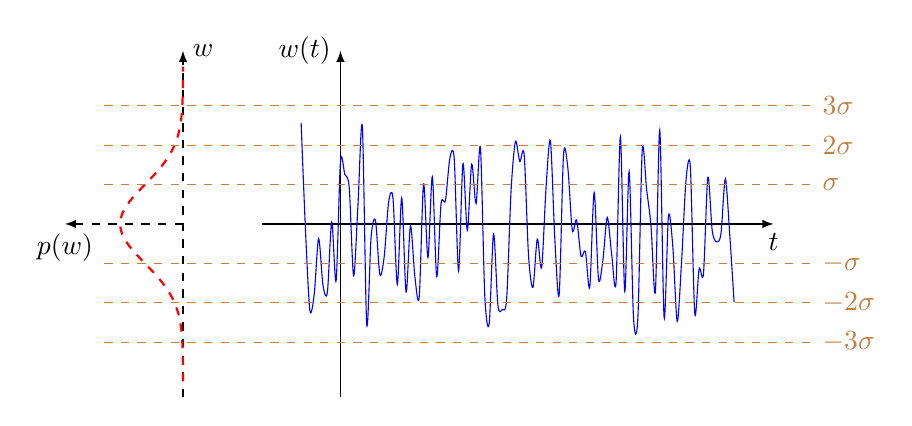
\begin{tikzpicture}
		\begin{scope}[shift={(0, 0)}]
			\draw[-latex] (-1,0) -- (5.5,0) node[below, align=center]{$t$};
			\draw[-latex] (0,-2.2) -- (0,2.2) node[left, align=right]{$w(t)$};
			\pgfmathsetseed{200};
			\draw[blue, smooth, domain=-0.5:5, samples=100] plot (\x,{1.3*rand});
		\end{scope}
		\begin{scope}[shift={(-2, 0)},rotate=90]
			\draw[-latex, dashed] (-2.2,0) -- (2.2,0) node[right, align=left]{$w$};
			\draw[-latex, dashed] (0,0) -- (0,1.5) node[below, align=center]{$p(w)$};
			\draw[red, thick, dashed, smooth, domain=-2:2, samples=50] plot (\x, {(1/(0.5*sqrt(2*pi)))*exp(-0.5*((\x)/0.5)^2)});
		\end{scope}
		\draw[brown, dashed] (-3, 1.5) -- ++(9,0) node[right,align=left]{$3 \sigma$};
		\draw[brown, dashed] (-3, 1.0) -- ++(9,0) node[right,align=left]{$2 \sigma$};
		\draw[brown, dashed] (-3, 0.5) -- ++(9,0) node[right,align=left]{$\sigma$};
		\draw[brown, dashed] (-3, -0.5) -- ++(9,0) node[right,align=left]{$-\sigma$};
		\draw[brown, dashed] (-3, -1.0) -- ++(9,0) node[right,align=left]{$-2 \sigma$};
		\draw[brown, dashed] (-3, -1.5) -- ++(9,0) node[right,align=left]{$-3 \sigma$};
	\end{tikzpicture}
	\caption[AWGN in the time domain]{\ac{AWGN} in the time domain}
\end{figure}

\begin{figure}[H]
	\centering
	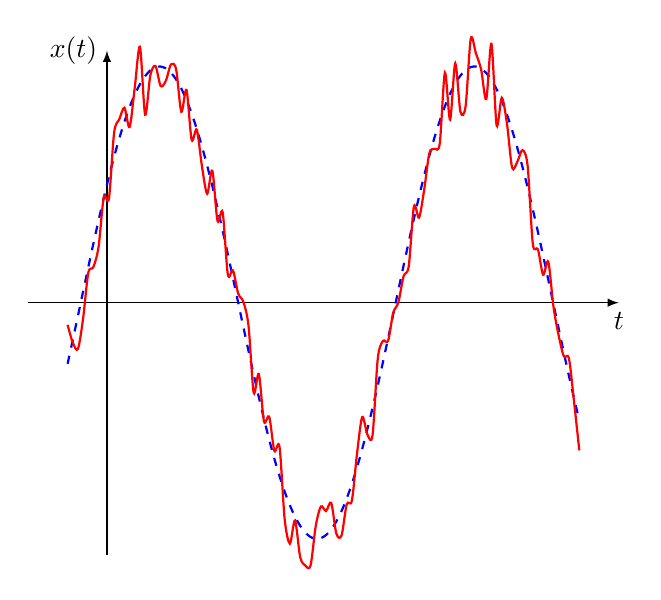
\begin{tikzpicture}
		\draw[-latex] (-1,0) -- (6.5,0) node[below, align=center]{$t$};
		\draw[-latex] (0,-3.2) -- (0,3.2) node[left, align=right]{$x(t)$};
		\draw[blue, thick, dashed, smooth, domain=-0.5:6, samples=100] plot (\x, {3*cos(360*\x/4-60)});
		\pgfmathsetseed{200};
		\draw[red, thick, smooth, domain=-0.5:6, samples=100] plot (\x, {3*cos(360*\x/4-60)+0.5*rand});
	\end{tikzpicture}
	\caption[Effect of AWGN on a signal (here monochromatic) in the time domain]{Effect of \ac{AWGN} on a signal (blue, here monochromatic) in the time domain. The resulting signal with the \ac{AWGN} is red.}
\end{figure}

\begin{figure}[H]
	\centering
	\begin{tikzpicture}
		\draw[-latex] (-3.2,0) -- (3.2,0) node[below, align=center]{$\Re$};
		\draw[-latex] (0,-3.2) -- (0,3.2) node[left, align=right]{$\Im$};
		\draw[blue, thick, dashed, -latex] (0:0) -- (60:2);
		\begin{scope}[shift={(60:2)}]
			\draw[brown, dashed] (0:0.4) arc(0:360:0.4);
			\draw[brown, dashed] (0:0.8) arc(0:360:0.8);
			\draw[brown, dashed] (0:1.2) arc(0:360:1.2);
			\draw[brown] (20:0.4) -- (20:2) node[right, align=left]{$\sigma$};
			\draw[brown] (45:0.8) -- (45:2.5) node[right, align=left]{$2 \sigma$};
			\draw[brown] (70:1.2) -- (70:3) node[right, align=left]{$3 \sigma$};
			\draw[brown, thick, -latex] (0:0) -- (130:0.5) node[anchor=east](W){};
		\end{scope}
		\draw[red, thick, -latex] (0,0) -- (W.east);
	\end{tikzpicture}
	\caption[Effect of AWGN on the phasor of a monochromatic signal (in the frequency domain)]{Effect of \ac{AWGN} (brown) on the phasor of a monochromatic signal (blue, in the frequency domain). The resulting signal with the \ac{AWGN} is red.}
\end{figure}

\subsection{Thermal Noise and Noise Floor}

The most important noise in electric circuits is \index{thermal noise} \textbf{thermal noise}.
\begin{itemize}
	\item Thermal noise is the corollary of oscillating atoms and molecules at the temperature $T$.
	\item The oscillation amplitude increases with increasing temperature. Consequently, the noise increases.
\end{itemize}

The noise \ac{PSD} $\mathrm{S}_{NN}$ is:
\begin{equation}
	\mathrm{S}_{NN}(\omega) = \frac{1}{2\pi} k_B T
\end{equation}
where $k_B = \SI{1.380649}{J/K}$ is the Boltzmann's constant. Or, for frequency instead of angular frequency:
\begin{equation}
	\mathrm{S}_{NN}(f) = k_B T
\end{equation}

\begin{itemize}
	\item When the thermal noise is band-limited, it has nearly a Gaussian or normal distribution. It is \ac{AWGN}.
	\item The noise has a finite power when it is band-limited.
\end{itemize}
The noise power of the band-limited thermal noise is
\begin{equation}
	\begin{split}
		P_N &= \int\limits_{\omega_1}^{\omega_2} \mathrm{S}_{NN} \; \mathrm{d} \omega \\
		 &= \frac{1}{2\pi} k_B T \underbrace{\left(\omega_2 - \omega_1\right)}_{= \Delta \omega} \\
		 &= k_B T \underbrace{\frac{\Delta \omega}{2\pi}}_{= \Delta f} \\
		 &= k_B T \Delta f
	\end{split}
\end{equation}
where $\Delta f$ is the \index{noise bandwidth} \textbf{noise bandwidth} in \si{Hz}.

\todo{noise voltage}

\paragraph{Noise Floor.}

The noise \ac{PSD} is small compared to the signals carrying information. Therefore, the logarithmic scale is used.

The noise \ac{PSD} level is
\begin{equation}
	L_{S,N} = \SI{10}{dBm/Hz} \log_{10} \left(\frac{k_B T}{\SI{1}{mW/Hz}}\right)
\end{equation}

\begin{itemize}
	\item The noise power is equally distributed over the frequency.
	\item Therefore, the \ac{PSD} is flat in the frequency domain, which is called \index{noise floor} \textbf{noise floor}.
\end{itemize}

\begin{fact}
	The noise \ac{PSD} or noise floor at room temperature (\SI{25}{\degreeCelsius} or $T = \SI{298.15}{K}$) is $L_{S,N} = \SI{-173.8}{dBm/Hz} \approx \SI{-174}{dBm/Hz}$.
\end{fact}

Band-limiting the noise, yields the noise power. The noise power is:
\begin{equation}
	\begin{split}
		L_{P,N} &= \SI{10}{dBm} \log_{10} \left(\frac{k_B T \Delta f}{\SI{1}{mW}}\right) \\
		 &= L_{S,N} + \SI{10}{dBHz} \log_{10} \left(\frac{\Delta f}{\SI{1}{Hz}}\right)
	\end{split}
\end{equation}

Here, the advantage of the logarithmic scale comes into play. For example, a \ac{LTE} signal with a bandwidth of $\Delta f_{LTE} = \SI{20}{MHz}$ has a noise power of $\SI{-174}{dBm/Hz} + \SI{73}{dBHz} = \SI{-101}{dBm}$.

\subsection{Signal-to-Noise Ratio and Noise Figure}

\paragraph {The Signal-to-Noise Ratio.}

Following scenario:
\begin{itemize}
	\item There is a signal at a frequency $\omega_0$ with a \ac{PSD} of $L_{S,X1}$ (for example indefinitely small peak $L_{S,X1} = \SI{-10}{dBm/Hz}$).
	\item The noise floor is the thermal noise $L_{S,N1}$ (for example $L_{S,N1} = \SI{-174}{dBm/Hz}$).
	\item The bandwidth considered is $\Delta f$ (for example $\Delta f = \SI{20}{MHz}$).
\end{itemize}

\begin{figure}[H]
	\centering
	\begin{tikzpicture}
		\draw[-latex] (-0.5,0) -- (5,0) node[below, align=center]{$f$\\ in $\si{Hz}$};
		\draw[-latex] (0,-10) -- (0,1) node[left, align=right]{$S(f)$\\ in $\si{dBm/Hz}$};
		
		\draw (2,0) -- ++(0,-0.1) node[below right, align=left]{$\omega_0$};
		
		\draw (0,-8.7) -- ++(-0.1,0) node[left, align=right]{$-174$};
		\draw (0,-0.5) -- ++(-0.1,0) node[left, align=right]{$-10$};
		
		\draw[red, thick] (0,-8.7) -- ++(5,0) node[above left, align=right]{Noise floor};
		\draw[blue, thick, -o] (2,-8.7) -- (2,-0.5) node[below right, align=left]{Signal};
	\end{tikzpicture}
	\caption[A signal including the AWGN]{A signal including the \ac{AWGN}}
\end{figure}

The noise power (level) is:
\begin{equation}
	\begin{split}
		P_{N1} &= \SI{1}{mW/Hz} 10^{\frac{L_{S,N1}}{\SI{10}{dBm/Hz}}} \cdot \Delta f \\
		L_{P,N1} &= L_{S,N1} + \SI{10}{dBHz} \log_{10} \left(\frac{\Delta f}{\SI{1}{Hz}}\right)
	\end{split}
\end{equation}
In this example, $L_{P,N1} = \SI{-101}{dBm}$.

The signal power is obtained by integrating the signal \ac{PSD} over the bandwidth:
\begin{equation}
	P_{X1} = \int\limits_{\Delta f} S_{XX}(\omega) \; \mathrm{d} \omega
\end{equation}

The signal \ac{PSD} in this example is:
\begin{equation*}
	S_{XX}(\omega) = \delta(\omega \pm \omega_0) \SI{1}{mW/Hz} 10^{\frac{L_{S,X1}}{\SI{10}{dBm/Hz}}}
\end{equation*}
In this example $P_{X1} \equiv L_{P,X1} = \SI{-10}{dBm}$.

\textit{Note:} the signal is just a indefinite small peak (Dirac delta function). All of its power is concentrated in its peak, so that the bandwidth does not matter. This signal does not exist in practise, but this is just an exemplary consideration.

\begin{definition}{Signal-to-noise ratio}
	The \index{signal-to-noise ratio} \textbf{\ac{SNR}} is the ratio between the signal power $P_{X}$ and the noise power $P_{N}$:
	\begin{equation}
		\mathrm{SNR} = \frac{P_{X}}{P_{N}}
	\end{equation}%
	\nomenclature[Ss]{$\mathrm{SNR}$}{Signal-to-noise ratio}
	
	Or in logarithmic scale
	\begin{equation}
		L_{\mathrm{SNR}} = \SI{10}{dB} \log_{10} \left(\frac{P_{X}}{P_{N}}\right) = L_{P,X} - L_{P,N}
	\end{equation}
\end{definition}

In this example, the \ac{SNR} is $L_{\mathrm{SNR},1} = \SI{91}{dB}$.

Often, the noise floor is defined to be \SI{91}{dBc}, which means that the noise is \SI{91}{dB} below the \index{carrier} \emph{carrier} -- the signal carrying the information.

\paragraph{\ac{SNR} Degradation.}

The signal including the \ac{AWGN} is applied to a system with a \index{gain} \textbf{gain} $G$.

Gain in logarithmic scale:
\begin{equation}
	L_G = \SI{10}{dB} \log_{10} \left(G\right)
\end{equation}

\begin{itemize}
	\item Positive log. gain $L_G > 0$ ($G > 1$): amplifier
	\item Negative log. gain $L_G < 0$ ($0 \leq G < 1$): attenuator
\end{itemize}

\begin{figure}[H]
	\centering
	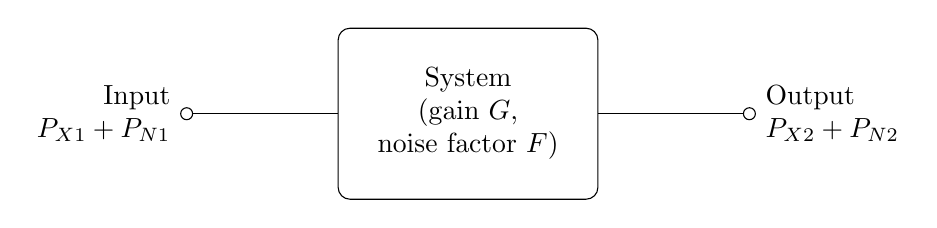
\begin{tikzpicture}
		\node[draw, block](Sys){System\\ (gain $G$,\\ noise factor $F$)};
		
		\draw[-o] (Sys.west) -- ++(-2,0) node[left, align=right]{Input\\ $P_{X1} + P_{N1}$};
		\draw[-o] (Sys.east) -- ++(2,0) node[right, align=left]{Output\\ $P_{X2} + P_{N2}$};
	\end{tikzpicture}
	\caption[A system with gain degrading the SNR]{A system with gain degrading the \ac{SNR}}
\end{figure}

The system
\begin{itemize}
	\item amplifies or attenuates \underline{both} the signal \underline{and} the noise, and
	\item adds intrinsic \ac{AWGN}.
\end{itemize}

The intrinsic \ac{AWGN} is thermal noise generated inside the system. This additional noise contribution shows up as an additional increase of the noise floor by a factor $F$ -- the \index{noise factor} \textbf{noise factor}. Or in logarithmic scale:
\begin{equation}
	L_F = \SI{10}{dB} \log_{10} \left(F\right)
\end{equation}

\begin{itemize}
	\item Amplification or attenuation of the signal:
	\begin{itemize}
		\item Linear scale: $P_{X2} = G P_{X1}$
		\item Logarithmic scale: $L_{P,X2} = L_{P,X1} + L_G$
	\end{itemize}
	\item Amplification or attenuation of the noise \underline{plus} intrinsic noise contribution:
	\begin{itemize}
		\item Linear scale: $P_{N2} = G F P_{N1}$
		\item Logarithmic scale: $L_{P,N2} = L_{P,N1} + L_G + L_F$
	\end{itemize}
\end{itemize}

The additional contribution of \ac{AWGN}, degrades the \ac{SNR} by $L_F$.

\begin{definition}{Noise figure and noise factor}
	The \index{noise factor} \textbf{noise factor} $F$ is the ratio of input \ac{SNR} $\mathrm{SNR}_i$ to output \ac{SNR} $\mathrm{SNR}_o$.
	\begin{equation}
		F = \frac{\mathrm{SNR}_i}{\mathrm{SNR}_o}
	\end{equation}
	
	In logarithmic scale, the ratio is expressed by the \index{noise figure} \textbf{noise figure} $L_F$.
	\begin{equation}
		L_F = \SI{10}{dB} \log_{10} \left(F\right) = L_{\mathrm{SNR},i} - L_{\mathrm{SNR},o}
	\end{equation}
\end{definition}

\begin{figure}[H]
	\centering
	\begin{tikzpicture}
		\begin{scope}[shift={(0,0)}]
			\draw[-latex] (-0.5,0) -- (5,0) node[below, align=center]{$f$\\ in $\si{Hz}$};
			\draw[-latex] (0,-10) -- (0,1.5) node[left, align=right]{$S(f)$\\ in $\si{dBm/Hz}$};
			
			\draw (2,0) -- ++(0,-0.1) node[below right, align=left]{$\omega_0$};
			
			\draw (0,-8.7) -- ++(-0.1,0) node[left, align=right]{$-174$};
			\draw (0,-0.5) -- ++(-0.1,0) node[left, align=right]{$-10$};
			
			\draw[red, thick] (0,-8.7) -- ++(5,0) node[above left, align=right](N1){Noise floor};
			\draw[blue, thick, -o] (2,-8.7) -- (2,-0.5) node[below right, align=left](X1){Signal};
		\end{scope}
		\begin{scope}[shift={(8,0)}]
			\draw[-latex] (-0.5,0) -- (5,0) node[below, align=center]{$f$\\ in $\si{Hz}$};
			\draw[-latex] (0,-10) -- (0,1.5) node[left, align=right]{$S(f)$\\ in $\si{dBm/Hz}$};
			
			\draw (2,0) -- ++(0,-0.1) node[below right, align=left]{$\omega_0$};
			
			\draw (0,-8.7) -- ++(-0.1,0) node[left, align=right]{$-174$};
			\draw (0,-7.7) -- ++(-0.1,0) node[left, align=right]{$-154$};
			\draw (0,-7.2) -- ++(-0.1,0) node[left, align=right]{$-144$};
			\draw (0,-0.5) -- ++(-0.1,0) node[left, align=right]{$-10$};
			\draw (0,0.5) -- ++(-0.1,0) node[left, align=right]{$+10$};
			
			\draw[red, dashed] (0,-7.7) -- ++(5,0) node[below left, align=right](Ng){Noise (gain only)};
			\draw[red, thick] (0,-7.2) -- ++(5,0) node[above left, align=right](N2){Noise floor};
			\draw[blue, thick, -o] (2,-7.2) -- (2,0.5) node[above right, align=left](X2){Signal};
		\end{scope}
		\begin{scope}[shift={(6,0)}]
			\draw (-0.5,-8.7) -- (0.5,-8.7);
			\draw[<->] (0,-8.7) -- (0,-7.7) node[midway, left, align=right]{$L_G$};
			\draw (-0.5,-7.7) -- (0.5,-7.7);
			\draw[<->] (0,-7.7) -- (0,-7.2) node[midway, left, align=right]{$L_F$};
			\draw (-0.5,-7.2) -- (0.5,-7.2);
			\draw (-0.5,-0.5) -- (0.5,-0.5);
			\draw[<->] (0,-0.5) -- (0,0.5) node[midway, left, align=right]{$L_G$};
			\draw (-0.5,0.5) -- (0.5,0.5);
		\end{scope}
	\end{tikzpicture}
	\caption[Degradation of the SNR]{Degradation of the \ac{SNR}}
\end{figure}

In our example:
\begin{itemize}
	\item System properties:
	\begin{itemize}
		\item Gain $L_G = \SI{20}{dB}$
		\item Noise figure $L_F = \SI{10}{dB}$
	\end{itemize}
	\item Output signal power $L_{X2} = \SI{+10}{dBm}$
	\item Output noise power $L_{X2} = \SI{-71}{dBm}$ ($\SI{-144}{dBm/Hz}$ at $\SI{20}{MHz}$)
	\item \ac{SNR} $L_{\mathrm{SNR},o} = \SI{81}{dB}$
\end{itemize}

\paragraph{Cascading Systems.}

In a cascade of systems, the gain $G$ and noise factor $F$ must be applied several times.

\begin{definition}{Friis formula}
	The total noise factor of a chain of $n$ devices can be calculated by the \index{Friis formula} \textbf{Friis formula}.
	\begin{equation}
		F_{\text{total}} = F_1 + \frac{F_2 - 1}{G_1} + \frac{F_3 - 1}{G_1 G_2} + \frac{F_4 - 1}{G_1 G_2 G_3} + \dots + \frac{F_n - 1}{G_1 G_2 \dots G_{n-1}}
	\end{equation}
	$F$ and $G$ are in linear scale (not logarithmic scale).
	
	\begin{figure}[H]
		\centering
		\begin{adjustbox}{scale=0.8}
			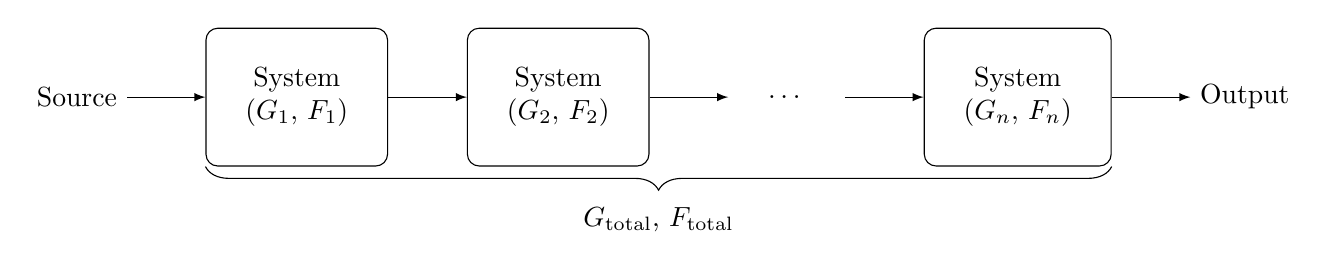
\begin{tikzpicture}
				\node[draw, block](S1){System\\ ($G_1$, $F_1$)};
				\node[draw, block,right=of S1](S2){System\\ ($G_2$, $F_2$)};
				\node[block,right=of S2](Sd){$\dots$};
				\node[draw, block,right=of Sd](Sn){System\\ ($G_n$, $F_n$)};
				
				\draw[latex-] (S1.west) -- ++(-1,0) node[left, align=right]{Source};
				\draw[-latex] (S1.east) -- (S2.west);
				\draw[-latex] (S2.east) -- (Sd.west);
				\draw[-latex] (Sd.east) -- (Sn.west);
				\draw[-latex] (Sn.east) -- ++(1,0) node[right, align=left]{Output};
				
				\draw[decorate, decoration={brace, amplitude=3mm, mirror}] (S1.south west) -- (Sn.south east) node[midway, anchor=north, yshift=-4mm]{$G_{\text{total}}$, $F_{\text{total}}$};
			\end{tikzpicture}
		\end{adjustbox}
	\end{figure}
\end{definition}

\textit{Remark:} The total chain gain is:
\begin{equation}
	G_{\text{total}} = G_1 G_2 \dots G_n = \prod_{i = 1}^{n} G_i
\end{equation}

\phantomsection
\addcontentsline{toc}{section}{References}
\printbibliography[heading=subbibliography]
\end{refsection}


\clearpage
% SPDX-License-Identifier: CC-BY-SA-4.0
%
% Copyright (c) 2020 Philipp Le
%
% Except where otherwise noted, this work is licensed under a
% Creative Commons Attribution-ShareAlike 4.0 License.
%
% Please find the full copy of the licence at:
% https://creativecommons.org/licenses/by-sa/4.0/legalcode

\phantomsection
\addcontentsline{toc}{section}{Exercise 3}
\section*{Exercise 3}

%%%%%%%%%%%%%%%%%%%%%%%%%%%%%%%%%%%%%%%%%%%%%%%%%%%%%%%%%%%%%%%%%%%%%%%%%%%%%%%
\begin{question}[subtitle={Stochastic Process}]
	A normally distributed random process produces the sequences $x_1(t)$, $x_2(t)$ and $x_3(t)$.
	\begin{table}[H]
		\centering
		\begin{tabular}{|l|r|r|r|r|r|r|r|r|r|r|}
			\hline
			$t$ & 0 & 1 & 2 & 3 & 4 & 5 & 6 & 7 & 8 & 9 \\
			\hline
			\hline
			$x_1(t)$ & 4.99 & 4.37 & 8.57 & 4.01 & 3.77 & 3.35 & 3.87 & 8.39 & 6.89 & 1.96 \\
			\hline
			$x_2(t)$ & 3.95 & 5.35 & 2.94 & 6.38 & 4.78 & 7.62 & 5.25 & 6.81 & 5.65 & 5.29 \\
			\hline
			$x_3(t)$ & 7.01 & 4.40 & 4.26 & 6.54 & 4.53 & 6.85 & 4.46 & 5.81 & 6.49 & 4.11 \\
			\hline
		\end{tabular}
	\end{table}
	\begin{tasks}
		\task
		Calculate the stochastic mean for each time instance!
		
		\task
		Calculate the temporal mean for each sequence!
		
		\task
		The process is ergodic with $\mu_x = 5.00$. However, why is the condition $\E\left\{\vect{x}\right\} = \overline{x} = \mu_x$ not fulfilled?
	\end{tasks}
\end{question}

\begin{solution}
	\begin{tasks}
		\task
		\begin{table}[H]
			\centering
			\begin{tabular}{|l|r|r|r|r|r|r|r|r|r|r|}
				\hline
				$t$ & 0 & 1 & 2 & 3 & 4 & 5 & 6 & 7 & 8 & 9 \\
				\hline
				\hline
				$\E\left\{\vect{x}(t)\right\}$ & 5.32 & 4.71 & 5.26 & 5.64 & 4.36 & 5.94 & 4.53 & 7.00 & 6.34 & 3.79 \\
				\hline
			\end{tabular}
		\end{table}
	
		\task
		\begin{itemize}
			\item $\overline{x_1} = 5.01$
			\item $\overline{x_1} = 5.40$
			\item $\overline{x_1} = 5.45$
		\end{itemize}
	
		\task
		\begin{itemize}
			\item There are only $N = 3$ sequences drawn from the random process. $\E\left\{\vect{x}\right\}$ will converge to $5.00$ for $N \rightarrow \infty$. $N = 3$ is too short.
			\item Each sequence is only $L = 10$ samples long. $\overline{x}$ will converge to $5.00$ for $L \rightarrow \infty$. $L = 10$ is too short.
		\end{itemize}
	\end{tasks}
\end{solution}

%%%%%%%%%%%%%%%%%%%%%%%%%%%%%%%%%%%%%%%%%%%%%%%%%%%%%%%%%%%%%%%%%%%%%%%%%%%%%%%
\begin{question}[subtitle={Cross-Correlation and Autocorrelation}]
	Two signals are given $f_1(t)$ and $f_2(t)$. The signals are value- and time-continuous. Ten samples are given. Both signals are zero for $t < -5$ and $t > 5$.
	\begin{table}[H]
		\centering
		\begin{tabular}{|l|r|r|r|r|r|r|r|r|r|r|r|}
			\hline
			$t$ & -5 & -4 & -3 & -2 & -1 & 0 & 1 & 2 & 3 & 4 & 5 \\
			\hline
			\hline
			$f_1(t)$ & 0 & 1 & 2 & 3 & 4 & 5 & 4 & 3 & 2 & 1 & 0 \\
			$f_2(t)$ & -1.34 & 0.30 & 14.54 & -1.54 & -3.03 & -1.72 & 14.16 & 2.70 & 1.17 & -2.44 & -4.66 \\
			\hline
		\end{tabular}
	\end{table}
	\begin{tasks}
		\task
		Calculate the cross-correlation
		\begin{equation*}
			\mathrm{R}_{f_1 f_2}(\tau) \approx \left(f_1 \star f_2\right)(\tau) = \sum\limits_{t=-5}^{5} f_1(t) f_2(t + \tau)
		\end{equation*}
		for $\tau = 0$, $\tau = 1$ and $\tau = 2$.
		
		\task
		Signal $f_2(t)$ contains signal $f_1(t)$ which is superimposed by noise. Using the values calculated in a), how much is the time $\Delta t$ lag between $f_1(t)$ and $f_2(t)$?
		
		\task
		Calculate the autocorrelation
		\begin{equation*}
			\mathrm{R}_{f_1 f_1}(\tau) \approx \left(f_1 \star f_1\right)(\tau) = \sum\limits_{t=-5}^{5} f_1(t) f_1(t + \tau)
		\end{equation*}
		for $\tau = -2$, $\tau = -1$, $\tau = 0$, $\tau = 1$ and $\tau = 2$.
		
		\task
		How much is the signal energy $E$ of $f_1(t)$?
		\begin{equation*}
			E \approx \frac{1}{T} \sum\limits_{t=-5}^{5} \left|f_1(t)\right|^2
		\end{equation*}
		with $T = 11$?
	\end{tasks}

	\textit{Remark:} Only samples of the functions with a spacing of $1$ are given. Therefore, the indefinite integrals of both cross-correlation and autocorrelation can be approximated using the sums.
\end{question}

\begin{solution}
	\begin{tasks}
		\task
		Full cross-correlation between $-10 \geq t \geq 10$. The cross-correlation is zero everywhere outside of the interval.
		\begin{table}[H]
			\centering
			\begin{tabular}{|l|r|r|r|r|r|r|r|r|r|}
				\hline
				$\tau$ & -10 & -9 & -8 & -7 & -6 & -5 & -4 & -3 & -2 \\
				\hline
				$\mathrm{R}_{f_1 f_2}(\tau)$ & $0.0$ & $-1.34$ & $-2.38$ & $11.12$ & $23.08$ & $32.01$ & $41.9$ & $65.35$ & $62.42$ \\
				\hline
				\hline
				$\tau$ & -1 & 0 & 1 & 2 & 3 & 4 & 5 & 6 & 7 \\
				\hline
				$\mathrm{R}_{f_1 f_2}(\tau)$ & $63.74$ & $68.68$ & $71.06$ & $45.42$ & $28.92$ & $8.54$ & $-9.99$ & $-20.92$ & $-17.69$ \\
				\hline
				\hline
				$\tau$ & 8 & 9 & 10 & & & & & & \\
				\hline
				$\mathrm{R}_{f_1 f_2}(\tau)$ & $-11.76$ & $-4.66$ & $0.0$ & & & & & & \\
				\hline
			\end{tabular}
		\end{table}
		\begin{itemize}
			\item $\left(f_1 \star f_2\right)(0) = 68.68$
			\item $\left(f_1 \star f_2\right)(1) = 71.06$
			\item $\left(f_1 \star f_2\right)(2) = 45.42$
		\end{itemize}
	
		\task
		\begin{itemize}
			\item The maximum value is at $\tau = 1$.
			\item $f_2(t)$ is delayed (negatively advanced) by $\Delta t = -1$ in relation to $f_1(t)$.
		\end{itemize}
	
		\task
		Full autocorrelation between $-10 \geq t \geq 10$. The autocorrelation is zero everywhere outside of the interval.
		\begin{table}[H]
			\centering
			\begin{tabular}{|l|r|r|r|r|r|r|r|r|r|r|r|}
				\hline
				$\tau$ & -10 & -9 & -8 & -7 & -6 & -5 & -4 & -3 & -2 & -1 & 0 \\
				\hline
				$\mathrm{R}_{f_1 f_1}(\tau)$ & 0 &  0 &  1 &  4 & 10 & 20 & 3. & 52 & 68 & 80 & 85 \\
				\hline
				\hline
				$\tau$ & 1 & 2 & 3 & 4 & 5 & 6 & 7 & 8 & 9 & 10 & \\
				\hline
				$\mathrm{R}_{f_1 f_1}(\tau)$ & 80 & 68 & 52 & 35 & 20 & 10 &  4 &  1 &  0 &  0 & \\
				\hline
			\end{tabular}
		\end{table}
		Only three values must be calculated:
		\begin{itemize}
			\item $\mathrm{R}_{f_1 f_1}(\tau)(-2) = 68$
			\item $\mathrm{R}_{f_1 f_1}(\tau)(-1) = 80$
			\item $\mathrm{R}_{f_1 f_1}(\tau)(0) = 85$
		\end{itemize}
		The other two values can be deducted from the symmetry rules:
		\begin{itemize}
			\item $\mathrm{R}_{f_1 f_1}(\tau)(1) = \mathrm{R}_{f_1 f_1}(\tau)(-1) = 80$
			\item $\mathrm{R}_{f_1 f_1}(\tau)(2) = \mathrm{R}_{f_1 f_1}(\tau)(-2) = 68$
		\end{itemize}
	
		\task
		\begin{itemize}
			\item It is not necessary to solve the sum again.
			\item The sum is $\mathrm{R}_{f_1 f_1}(\tau)(0)$.
			\item The energy is
			\begin{equation*}
				E = \frac{1}{11} \mathrm{R}_{f_1 f_1}(\tau)(0) = 7.23
			\end{equation*}
		\end{itemize}
	\end{tasks}
\end{solution}


%%%%%%%%%%%%%%%%%%%%%%%%%%%%%%%%%%%%%%%%%%%%%%%%%%%%%%%%%%%%%%%%%%%%%%%%%%%%%%%
\begin{question}[subtitle={Power Spectral Density}]
	Are the following statements about the power spectral density (PSD) true or false? If false, correct the statement!
	\begin{tasks}
		\task
		The PSD is measure for the fraction of power which is located at a certain frequency.
		
		\task
		The unit of the PSD is the same as the signal.
		
		\task
		The PSD is even, if the signal is purely real-valued.
		
		\task
		The PSD is odd, if the signal is complex-valued.
		
		\task
		The PSD is always real-valued.
		
		\task
		The PSD can be used to determine the output signal of an LTI system in amplitude and phase.
		
	\end{tasks}
\end{question}

\begin{solution}
	\begin{tasks}
		\task
		True. The signal power can be obtained by integration of the PSD over all frequencies.
		\begin{equation*}
			P = \int\limits_{-\infty}^{\infty} \mathrm{S}_{xx}(\omega) \; \mathrm{d} \omega
		\end{equation*}
		
		\task
		False.
		\begin{equation*}
			\left(\text{Unit of PSD}\right) = \frac{\left(\text{Unit of signal}\right)^2}{\left(\text{Unit of frequency}\right)}
		\end{equation*}
		
		For example \si{W/Hz}. Never \si{W} only, because it is the density of the power across the frequency.
		
		\task
		True
		
		\task
		False. There are no symmetry rules for the PSD, if the signal is complex-valued.
		
		\task
		True.
		\begin{itemize}
			\item The autocorrelation function is always Hermitian.
			\item The Fourier transform of a Hermitian function is always real-valued.
			\item Therefore, the PSD is real-valued.
		\end{itemize}
		
		\task
		False.
		\begin{itemize}
			\item Only the amplitude can be calculated.
			\item The phase information of the system is lost by squaring the absolute value of the transfer funtion.
			\item Furthermore, the PSD does not contain phase information of the signal.
		\end{itemize}
	\begin{equation*}
		\mathrm{S}_{yy}(\omega) = \left|\underline{H}\left(j \omega\right)\right|^2 \cdot \mathrm{S}_{xx}(\omega)
	\end{equation*}
	\end{tasks}
\end{solution}


%%%%%%%%%%%%%%%%%%%%%%%%%%%%%%%%%%%%%%%%%%%%%%%%%%%%%%%%%%%%%%%%%%%%%%%%%%%%%%%
\begin{question}[subtitle={Decibel}]
	\begin{tasks}
		\task
		Convert to logarithmic scale or vice versa!
		\begin{enumerate}
			\item \SI{2}{mW}, $P_0 = \SI{1}{mW}$
			\item \SI{2}{V}, $U_0 = \SI{1}{V}$
			\item \num{400000}
			\item \SI{5}{GHz}, $f_0 = \SI{1}{Hz}$
			\item \SI{8}{fW/MHz}, $P_0 = \SI{1}{mW}$
			\item \SI{5}{dB\micro\volt}
			\item \SI{-10}{dBm}
		\end{enumerate}
	
		\task
		Convert to logarithmic scale or vice versa!
		\begin{enumerate}
			\item $1$
			\item $2$
			\item $4$
			\item $0.5$
			\item $0.25$
			\item $10$
			\item $100$
			\item $0.1$
			\item $0.01$
			\item $500$
			\item $0.04$
		\end{enumerate}
	
		\task
		A signal is transmitted with a power of \SI{13}{dBm}. The signal is attenuated by \SI{86}{dB} on its way to the receiver. Assume that a ohmic resistance of \SI{50}{\ohm} is connected to the antenna. What voltage can be measured at this resistance? Give your result in linear and logarithmic scale!
	\end{tasks}
\end{question}

\begin{solution}
	\begin{tasks}
		\task
		\begin{enumerate}
			\item $\SI{10}{dBm} \cdot \log_{10} \left(\frac{\SI{2}{mW}}{\SI{1}{mW}}\right) = \SI{3}{dBm}$
			\item $\SI{20}{dBV} \cdot \log_{10} \left(\frac{\SI{2}{V}}{\SI{1}{V}}\right) = \SI{6}{dBV}$ (20 instead of 10 for voltages and currents)
			\item $\SI{10}{dB} \cdot \log_{10} \left(400000\right) = \SI{53}{dB}$
			\item $\SI{10}{dBHz} \cdot \log_{10} \left(\frac{\SI{5}{GHz}}{\SI{1}{Hz}}\right) = \SI{97}{dbHz}$
			\item $\SI{10}{dBm/Hz} \cdot \log_{10} \left(\frac{\SI{8}{fW/MHz}}{\SI{1}{mW/Hz}}\right) = \SI{10}{dBm/Hz} \cdot \log_{10} \left(\frac{10^{-6} \cdot \SI{8}{fW/Hz}}{\SI{1}{mW/Hz}}\right) = \SI{-171}{dBm/Hz}$
			\item $\SI{1}{\micro\volt} \cdot 10^{\SI{5}{dB\micro\volt} / 20} = \SI{1.8}{\micro\volt}$
			\item $\SI{1}{mW} \cdot 10^{\SI{-10}{dBm} / 10} = \SI{100}{\micro.W}$
		\end{enumerate}
	
		\task
		\begin{enumerate}
			\item $\SI{0}{dB}$
			\item $\SI{3}{dB}$
			\item $\SI{6}{dB}$, Hint: $4 = 2 \cdot 2 \equiv \SI{3}{dB} + \SI{3}{dB} = \SI{6}{dB}$
			\item $\SI{-3}{dB}$
			\item $\SI{-6}{dB}$, Hint: $0.25 = 0.5 \cdot 0.5 \equiv \SI{-3}{dB} + \SI{-3}{dB} = \SI{-6}{dB}$
			\item $\SI{10}{dB}$
			\item $\SI{20}{dB}$
			\item $\SI{-10}{dB}$
			\item $\SI{-20}{dB}$
			\item $\SI{27}{dB}$, Hint: $50 = 10 \cdot 10 \cdot 10 \cdot 0.5 \equiv \SI{10}{dB} + \SI{10}{dB} + \SI{10}{dB} - \SI{3}{dB} = \SI{27}{dB}$
			\item $\SI{-14}{dB}$, Hint: $0.04 = 0.1 \cdot 0.1 \cdot 2 \cdot 2 \equiv \SI{-10}{dB} + \SI{-10}{dB} + \SI{3}{dB} + \SI{3}{dB} = \SI{-14}{dB}$
		\end{enumerate}
		Remember these rules as an RF engineer! You will need them often. ;)
		
		\task
		Power at the receiver antenna:
		\begin{equation*}
			\SI{13}{dBm} \underbrace{- \SI{86}{dB}}_{\text{Atennuation}} = \SI{-73}{dBm}
		\end{equation*}
		
		\begin{itemize}
			\item 1st way: Convert to linear scale, then back to logarithmic scale
			\begin{equation*}
				\begin{split}
					\SI{-73}{dBm} &\equiv \SI{50.1}{pW} \\
					U = \sqrt{P \cdot R} &= \sqrt{\SI{50.1}{pW} \cdot \SI{50}{\ohm}} = \SI{50}{\micro\volt} \\
					\SI{50}{\micro\volt} &\equiv \underbrace{\SI{20}{dB\micro\volt}}_{\text{Attention!}} \cdot \log_{10}\left(\frac{\SI{50}{\micro\volt}}{\SI{1}{\micro\volt}}\right) = \SI{34}{dB\micro\volt}
				\end{split}
			\end{equation*}
			\item 2nd way: Convert everything to logarithmic scale. The multiplication of power and resistance must happen with ``pure'' SI units.
			\begin{equation*}
			\begin{split}
				\SI{50}{\ohm} &\equiv \SI{10}{dB\ohm} \cdot \log_{10} \left(\frac{\SI{50}{\ohm}}{\SI{1}{\ohm}}\right) = \SI{17}{dB\ohm} \\
				\SI{-73}{dBm} \underbrace{- \SI{30}{dB}}_{\text{\si{mW} to \si{W}}} &= \SI{-103}{dBW} \quad \text{SI unit!} \\
				\SI{-103}{dBW} + \SI{17}{dB\ohm} &= \SI{-86}{dBV} \quad \text{SI unit!} \\
				\SI{-86}{dBV} \underbrace{+ \SI{120}{dB}}_{\text{\si{V} to \si{\micro\volt}}} &= \SI{34}{dB\micro\volt} \\
				\SI{34}{dB\micro\volt} &\equiv \SI{1}{\micro\volt} \cdot 10^{\frac{34}{20}} = \SI{50}{\micro\volt}
			\end{split}
			\end{equation*}
		\end{itemize}
	
		\textit{Remarks:} Conversion of different SI prefixes:
		\begin{itemize}
			\item From \si{mW} to \si{W}:
			\begin{equation*}
				\begin{split}
					\SI{1}{mW} &= \SI{0.001}{W} \\
					\SI{10}{dB} \cdot \log_{10}\left(\frac{\SI{0.001}{W}}{\SI{1}{mW}}\right) &= \SI{-30}{dB}
				\end{split}
			\end{equation*}
			\item From \si{V} to \si{\micro\volt}:
			\begin{equation*}
				\begin{split}
					\SI{1}{V} &= \SI{1000000}{\micro\volt} \\
					\SI{20}{dB} \cdot \log_{10}\left(\frac{\SI{1000000}{\micro\volt}}{\SI{1}{V}}\right) &= \SI{120}{dB}
				\end{split}
			\end{equation*}
		\end{itemize}
	\end{tasks}
\end{solution}

%%%%%%%%%%%%%%%%%%%%%%%%%%%%%%%%%%%%%%%%%%%%%%%%%%%%%%%%%%%%%%%%%%%%%%%%%%%%%%%
\begin{question}[subtitle={Noise}]
	The following system is given:
	\begin{figure}[H]
		\centering
		\begin{adjustbox}{scale=0.7}
			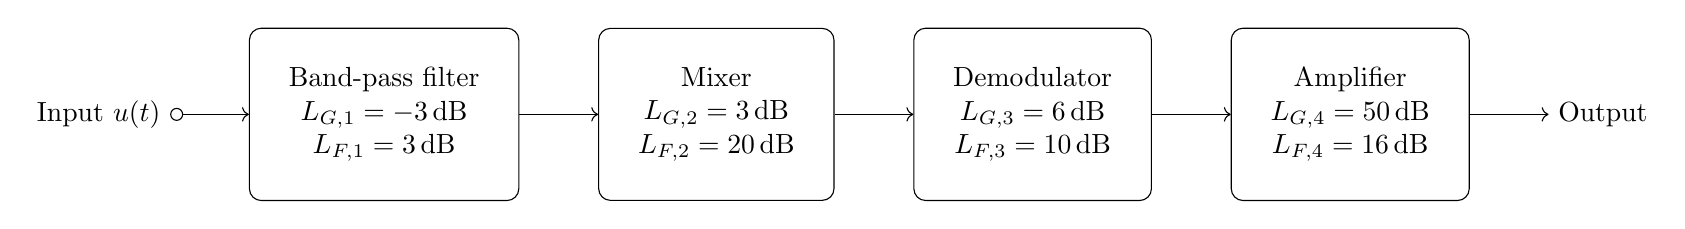
\begin{tikzpicture}
				\node[draw, block] (BPF){Band-pass filter\\ $L_{G,1} = \SI{-3}{dB}$\\ $L_{F,1} = \SI{3}{dB}$};
				\node[draw, block, right=of BPF] (Mix){Mixer\\ $L_{G,2} = \SI{3}{dB}$\\ $L_{F,2} = \SI{20}{dB}$};
				\node[draw, block, right=of Mix] (Demod){Demodulator\\ $L_{G,3} = \SI{6}{dB}$\\ $L_{F,3} = \SI{10}{dB}$};
				\node[draw, block, right=of Demod] (Amp){Amplifier\\ $L_{G,4} = \SI{50}{dB}$\\ $L_{F,4} = \SI{16}{dB}$};
				
				\draw[o->] ([xshift=-1cm]BPF.west) node[left,align=right]{Input $u(t)$} -- (BPF.west);
				\draw[->] (BPF.east) -- (Mix.west);
				\draw[->] (Mix.east) -- (Demod.west);
				\draw[->] (Demod.east) -- (Amp.west);
				\draw[->] (Amp.east) -- ([xshift=1cm]Amp.east) node[right,align=left]{Output};
			\end{tikzpicture}
		\end{adjustbox}
	\end{figure}
	\begin{itemize}
		\item The band-pass filter has an input impedance of $\SI{50}{\ohm}$.
		\item The band-pass filter has a bandwidth of $\SI{2}{MHz}$.
		\item All system components are at room temperature: \SI{25}{\degreeCelsius}.
	\end{itemize}
	The input signal is:
	\begin{equation*}
		u(t) = \SI{70.71}{\micro\volt} \cdot \cos\left(\omega_0 t\right)
	\end{equation*}
	
	Give all results in the logarithmic scale!
	\begin{tasks}
		\task
		What is the signal power, the thermal noise power and the SNR at the input?
		
		\task
		What is the overall noise figure and overall gain of the chain? What is the signal power, the thermal noise power and the SNR at the output of the chain?
		
		\task
		Now a low noise amplifier is placed in front of the mixer. The gain of the last amplifier is reduced, so that the overall gain does not change.
		\begin{figure}[H]
			\centering
			\begin{adjustbox}{scale=0.5}
				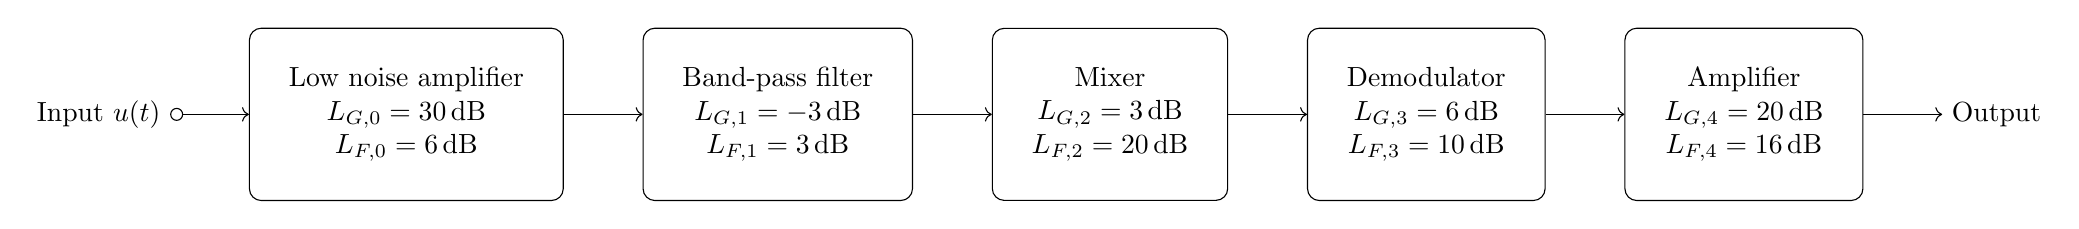
\begin{tikzpicture}
					\node[draw, block] (Amp){Low noise amplifier\\ $L_{G,0} = \SI{30}{dB}$\\ $L_{F,0} = \SI{6}{dB}$};
					\node[draw, block, right=of Amp] (BPF){Band-pass filter\\ $L_{G,1} = \SI{-3}{dB}$\\ $L_{F,1} = \SI{3}{dB}$};
					\node[draw, block, right=of BPF] (Mix){Mixer\\ $L_{G,2} = \SI{3}{dB}$\\ $L_{F,2} = \SI{20}{dB}$};
					\node[draw, block, right=of Mix] (Demod){Demodulator\\ $L_{G,3} = \SI{6}{dB}$\\ $L_{F,3} = \SI{10}{dB}$};
					\node[draw, block, right=of Demod] (Amp2){Amplifier\\ $L_{G,4} = \SI{20}{dB}$\\ $L_{F,4} = \SI{16}{dB}$};
					
					\draw[o->] ([xshift=-1cm]Amp.west) node[left,align=right]{Input $u(t)$} -- (Amp.west);
					\draw[->] (Amp.east) -- (BPF.west);
					\draw[->] (BPF.east) -- (Mix.west);
					\draw[->] (Mix.east) -- (Demod.west);
					\draw[->] (Demod.east) -- (Amp2.west);
					\draw[->] (Amp2.east) -- ([xshift=1cm]Amp2.east) node[right,align=left]{Output};
				\end{tikzpicture}
			\end{adjustbox}
		\end{figure}
		For this new constellation: What is the overall noise figure and overall gain of the chain? What is the signal power, the thermal noise power and the SNR at the output of the chain?
	\end{tasks}
\end{question}

\begin{solution}
	\begin{tasks}
		\task
		\begin{itemize}
			\item The RMS value of the signals is: $\frac{\SI{70.71}{\micro\volt}}{\sqrt{2}} = \SI{50}{\micro\volt}$
			\item At $\SI{50}{\ohm}$, this yields a power of: $P = \frac{U^2}{R} = \SI{50}{pW} \equiv L_{P,S} = \SI{-73}{dBm}$
			\item The noise floor at room temperature is: $k_B T \equiv \SI{-174}{dBm/Hz}$
			\item The filter's bandwidth is: $\SI{63}{dBHz}$
			\item The noise power is: $k_B T \Delta f \equiv L_{P,N} = \SI{-174}{dBm/Hz} + \SI{63}{dBHz} = \SI{-111}{dBm}$
			\item The SNR is: $L_{\mathrm{SNR}} = L_{P,S} - L_{P,N} = \SI{-73}{dBm} - (\SI{-111}{dBm}) = \SI{38}{dBm}$
		\end{itemize}
	
		\task
		Convert to linear scale:
		\begin{itemize}
			\item $G_1 = 0.5$
			\item $F_1 = 2$
			\item $G_2 = 2$
			\item $F_2 = 100$
			\item $G_3 = 4$
			\item $F_3 = 10$
			\item $G_4 = 100000$
			\item $F_4 = 40$
		\end{itemize}
	
		Using the Friis formula:
		\begin{equation*}
			\begin{split}
				F_{\text{total}} &= F_1 + \frac{F_2 - 1}{G_1} + \frac{F_3 - 1}{G_1 G_2} + \frac{F_4 - 1}{G_1 G_2 G_3} \\
				 &= 218 \\
				L_{F,\text{total}} &= \SI{23.4}{dB}
			\end{split}
		\end{equation*}
		Overall gain:
		\begin{equation*}
			L_{G,\text{total}} = \SI{-3}{dB} + \SI{3}{dB} + \SI{6}{dB} + \SI{50}{dB} = \SI{56}{dB}
		\end{equation*}
		\begin{itemize}
			\item Output signal power: $\SI{-73}{dBm} + L_{G,\text{total}} = \SI{-17}{dBm}$
			\item Output noise power: $\SI{-111}{dBm} + L_{G,\text{total}} + L_{F,\text{total}} = \SI{-31.6}{dBm}$
			\item Output SNR: $\SI{38}{dBm} - L_{F,\text{total}} = \SI{14.6}{dB}$
		\end{itemize}
	
		\task
		Convert to linear scale:
		\begin{itemize}
			\item $G_0 = 1000$
			\item $F_0 = 4$
			\item $G_1 = 0.5$
			\item $F_1 = 2$
			\item $G_2 = 2$
			\item $F_2 = 100$
			\item $G_3 = 4$
			\item $F_3 = 10$
			\item $G_4 = 10$
			\item $F_4 = 40$
		\end{itemize}
	
		Using the Friis formula:
		\begin{equation*}
			\begin{split}
				F_{\text{total}} &= F_0 + \frac{F_1 - 1}{G_0} + \frac{F_2 - 1}{G_0 G_1} + \frac{F_3 - 1}{G_0 G_1 G_2} + \frac{F_4 - 1}{G_0 G_1 G_2 G_3} \\
				 &= 4.22 \\
				L_{F,\text{total}} &= \SI{6.3}{dB}
			\end{split}
		\end{equation*}
		Overall gain:
		\begin{equation*}
			L_{G,\text{total}} = \SI{50}{dB} + \SI{-3}{dB} + \SI{3}{dB} + \SI{6}{dB} = \SI{56}{dB}
		\end{equation*}
		\begin{itemize}
			\item Output signal power: $\SI{-73}{dBm} + L_{G,\text{total}} = \SI{-17}{dBm}$
			\item Output noise power: $\SI{-111}{dBm} + L_{G,\text{total}} + L_{F,\text{total}} = \SI{-48.7}{dBm}$
			\item Output SNR: $\SI{38}{dBm} - L_{F,\text{total}} = \SI{31.7}{dB}$
		\end{itemize}
	
		\textbf{Conclusion:}
		\begin{itemize}
			\item Placing the low noise amplifier in front of the chain, gives a much better ($\SI{16.1}{dB}$) SNR. The gain is equal.
			\item The overall noise figure is dominated by the first component in the chain.
			\item In this constellation, first component is a low noise amplifier with high gain and low noise figure.
			\item The high gain scales down the noise contribution of the components following in the chain.
			\item Therefore, it is always feasible to place a low noise amplifier (high gain, low noise) to the front of the chain.
		\end{itemize}
	\end{tasks}
\end{solution}

\begin{question}[subtitle={Python Programming: Cross-correlation}]
Solve all tasks in Python!

Three signal samples are provided along with this exercise. Which one correlates most with the Gauss pulse given in the Python template file?

Make plots and decide from them!
\end{question}

\begin{solution}
\end{solution}



%%%%%%%%%%%%%%%%%%%%%%%%%%%%%%%%%%%%%%%%%%%%%%%%%%%%%%%%%%%%%%%%%%%%%%%%%%%%%%%
%\begin{question}[subtitle={Decibel}]
%	\begin{tasks}
%	\end{tasks}
%\end{question}
%
%\begin{solution}
%	\begin{tasks}
%	\end{tasks}
%\end{solution}

\clearpage

% SPDX-License-Identifier: CC-BY-SA-4.0
%
% Copyright (c) 2020 Philipp Le
%
% Except where otherwise noted, this work is licensed under a
% Creative Commons Attribution-ShareAlike 4.0 License.
%
% Please find the full copy of the licence at:
% https://creativecommons.org/licenses/by-sa/4.0/legalcode

\chapter{Sampling and Time-Discrete Signals and Systems}

\begin{refsection}

\section{Time-Discrete Signals}

\subsection{Ideal Sampling}

\begin{figure}[H]
	\centering
	\begin{tikzpicture}
		\begin{axis}[
			height={0.25\textheight},
			width=0.6\linewidth,
			scale only axis,
			xlabel={$t$},
			ylabel={$x$},
			%grid style={line width=.6pt, color=lightgray},
			%grid=both,
			grid=none,
			legend pos=north west,
			axis y line=middle,
			axis x line=middle,
			every axis x label/.style={
				at={(ticklabel* cs:1.05)},
				anchor=north,
			},
			every axis y label/.style={
				at={(ticklabel* cs:1.05)},
				anchor=east,
			},
			%xmin=0,
			%xmax=7,
			%ymin=0,
			%ymax=3,
			%xtick={0, 1, ..., 6},
			%ytick={0, 0.5, ..., 2.5},
			xmin=0,
			xmax=6.5,
			xtick={0, 1, ..., 6},
			xticklabels={$0$, $T_S$, $2 T_S$, $3 T_S$, $4 T_S$, $5 T_S$, $6 T_S$},
		]
			\addplot[smooth, blue, dashed] coordinates {(0, 1.1) (1, 1.8) (2, 2.1) (3, 1.0) (4, 0.8) (5, 1.7) (6, 2.4)};
			\addlegendentry{$\underline{x}(t)$};
			\addplot[red, thick] coordinates {(0, 0) (0, 1.1)};
			\addplot[red, thick] coordinates {(1, 0) (1, 1.8)};
			\addplot[red, thick] coordinates {(2, 0) (2, 2.1)};
			\addplot[red, thick] coordinates {(3, 0) (3, 1.0)};
			\addplot[red, thick] coordinates {(4, 0) (4, 0.8)};
			\addplot[red, thick] coordinates {(5, 0) (5, 1.7)};
			\addplot[red, thick] coordinates {(6, 0) (6, 2.4)};
			\addplot[only marks, red, thick, mark=o] coordinates {(0, 1.1) (1, 1.8) (2, 2.1) (3, 1.0) (4, 0.8) (5, 1.7) (6, 2.4)};
			\addlegendentry{$\underline{x}_S(t)$};
		\end{axis}
	\end{tikzpicture}
	\caption{Sampling of a time-continuous signal}
	\label{fig:ch04:sampling_of_signal}
\end{figure}

Sampling:
\begin{itemize}
	\item Sampling is converting a time-continuous signal $\underline{x}(t)$ to a time-discrete signal $\underline{x}[n]$.
	\item Samples are periodically taken out of the original signal.
\end{itemize}

Nomenclature:
\begin{itemize}
	\item The original time-continuous signal is $\underline{x}(t)$. The continuous time variable $t \in \mathbb{R}$ is a continuous real number.
	\item The sampled signal is $\underline{x}[n]$. The discrete time variable $n \in \mathbb{Z}$ is a (discrete) integer number.
	\item Round parenthesis is used for time-continuous signals. Square parenthesis is used for time-discrete signals.
\end{itemize}

Sampling parameters:
\begin{itemize}
	\item The time instances, at which the samples are taken out, are equidistant.
	\item The period between the samples is the \index{sampling period} \textbf{sampling period} $T_S$.
	\item The inverse of the sampling period is the \index{sampling rate} \textbf{sampling rate} $f_S$.
	\begin{equation}
		f_S = \frac{1}{T_S}
	\end{equation}
	\item The \index{sampling angular frequency} \textbf{sampling angular frequency} $\omega_S$.
	\begin{equation}
		\omega_S = \frac{2 \pi}{T_S}
	\end{equation}
\end{itemize}

Ideal sampling:
\begin{itemize}
	\item The samples are ideally equidistant. The sampling period $T_S$ is constant and is \underline{not} subject to fluctuations.
	\item The sample has the value of the original signal $\underline{x}(t)$ at \underline{exactly} the time instance where has been taken.
\end{itemize}
Some corollaries can be deducted from these two points:
\begin{itemize}
	\item The sampled signal $\underline{x}_S(n T_S)$ at the discrete time $n$ is the value of the original signal at time $t = n T_S$.
	\begin{equation}
		\underline{x}[n] = \underline{x}\left(n T_S\right)
	\end{equation}
	\item The sampled signal $\underline{x}_S(t)$ consists of a chain of equidistant, indefinitely narrow pulses.
	\begin{itemize}
		\item The pulses are equidistant with $T_S$.
		\item The pulses have the value of $\underline{x}\left(n T_S\right)$ as their amplitudes.
		\item The value of the sampled signal is zero in between the pulses.
		\begin{equation}
			\underline{x}_S(t) = \begin{cases}
				\underline{x}\left(n T_S\right) & \quad \forall \; t = n T_S, n \in \mathbb{Z}, \\
				0 & \quad \forall \; n T_S < t < \left(n+1\right) T_S, n \in \mathbb{Z}.
			\end{cases}
		\end{equation}
	\end{itemize}
\end{itemize}

\subsubsection{Dirac comb}

We know already indefinitely narrow pulses. They are Dirac delta functions $\delta\left(t - n T_S\right)$.

Taking out \underline{exactly one} sample out of $\underline{x}(t)$ is a multiplication of $\underline{x}(t)$ with $\delta\left(t - n T_S\right)$.
\begin{equation}
	\underline{x}_{S,n}(t) = \underline{x}(t) \delta\left(t - n T_S\right)
	\label{eq:ch4:one_sample_1}
\end{equation}
The Dirac delta function is zero expect at $t = n T_S$. So, \eqref{eq:ch4:one_sample_1} can be further reduced.
\begin{equation}
	\underline{x}_{S,n}(t) = \underline{x}(n T_S) \delta\left(t - n T_S\right)
	\label{eq:ch4:one_sample_2}
\end{equation}

\begin{figure}[H]
	\centering
	\begin{tikzpicture}
		\begin{axis}[
			height={0.25\textheight},
			width=0.6\linewidth,
			scale only axis,
			xlabel={$t$},
			ylabel={$x$},
			%grid style={line width=.6pt, color=lightgray},
			%grid=both,
			grid=none,
			legend pos=north west,
			axis y line=middle,
			axis x line=middle,
			every axis x label/.style={
				at={(ticklabel* cs:1.05)},
				anchor=north,
			},
			every axis y label/.style={
				at={(ticklabel* cs:1.05)},
				anchor=east,
			},
			%xmin=0,
			%xmax=7,
			%ymin=0,
			%ymax=3,
			%xtick={0, 1, ..., 6},
			%ytick={0, 0.5, ..., 2.5},
			xmin=0,
			xmax=6.5,
			xtick={0, 1, ..., 6},
			xticklabels={$0$, $T_S$, $2 T_S$, $3 T_S$, $4 T_S$, $5 T_S$, $6 T_S$},
		]
			\addplot[smooth, blue, dashed] coordinates {(0, 1.1) (1, 1.8) (2, 2.1) (3, 1.0) (4, 0.8) (5, 1.7) (6, 2.4)};
			\addlegendentry{$\underline{x}(t)$};
			\addplot[red, thick] coordinates {(2, 0) (2, 2.1)};
			\addplot[only marks, red, thick, mark=o] coordinates {(2, 2.1)};
			\addlegendentry{$\underline{x}_{S,n}(t)$};
		\end{axis}
	\end{tikzpicture}
	\caption[Taking out exactly one sample out of $\underline{x}(t)$]{Taking out exactly one sample out of $\underline{x}(t)$ -- in this example $n = 2$.}
\end{figure}

To obtain the sampled signal, the sampling process $\underline{x}_{S,n}(t)$ \eqref{eq:ch4:one_sample_1} needs to be repeated for each $n \in \mathbb{Z}$. All individual sample processes $\underline{x}_{S,n}(t)$ are then superimposed to form the complete sampled signal $\underline{x}_S(t)$.
\begin{equation}
	\begin{split}
		\underline{x}_S(t) &= \sum\limits_{n = -\infty}^{\infty} \underline{x}_{S,n}(t) \\
		 &= \sum\limits_{n = -\infty}^{\infty} \underline{x}\left(t\right) \delta\left(t - n T_S\right) \\
		 &= \underline{x}\left(t\right) \cdot \underbrace{\sum\limits_{n = -\infty}^{\infty} \delta\left(t - n T_S\right)}_{= \Sha_{T_S}(t)}
	\end{split}
\end{equation}

The sum of Dirac delta functions
\begin{itemize}
	\item forms a series of equidistant pulses repeating at a period of $T_S$,
	\item is called \index{Dirac comb} \textbf{Dirac comb} $\Sha_{T_S}(t)$ or \index{impulse train} \textbf{impulse train}.
\end{itemize}

\begin{definition}{Dirac comb}
	The \index{Dirac comb} \textbf{Dirac comb} $\Sha_{T}(t)$ or \index{impulse train} \textbf{impulse train} is:
	\begin{equation}
		\Sha_{T}(t) = \sum\limits_{n = -\infty}^{\infty} \delta\left(t - n T\right)
		\label{eq:ch04:dirac_comb}
	\end{equation}
	$T$ is the period of the equidistant Dirac pulses.
	
	It is a periodic signal and can be decomposed using the Fourier analysis:
	\begin{equation}
		\Sha_{T}(t) = \frac{1}{T} \sum\limits_{n = -\infty}^{\infty} e^{j n \frac{2 \pi}{T} t}
		\label{eq:ch04:dirac_comb_fourier_series}
	\end{equation}
	
	\begin{figure}[H]
		\centering
		\begin{tikzpicture}
			\begin{axis}[
				height={0.15\textheight},
				width=0.9\linewidth,
				scale only axis,
				xlabel={$t$},
				ylabel={$\Sha_{T_S}(t)$},
				%grid style={line width=.6pt, color=lightgray},
				%grid=both,
				grid=none,
				legend pos=north east,
				axis y line=middle,
				axis x line=middle,
				every axis x label/.style={
					at={(ticklabel* cs:1.05)},
					anchor=north,
				},
				every axis y label/.style={
					at={(ticklabel* cs:1.05)},
					anchor=east,
				},
				xmin=-5.5,
				xmax=5.5,
				ymin=0,
				ymax=1.2,
				xtick={-5, -4, ..., 5},
				xticklabels={$-5 T_S$, $-4 T_S$, $-3 T_S$, $-2 T_S$, $- T_S$, $0$, $T_S$, $2 T_S$, $3 T_S$, $4 T_S$, $5 T_S$},
				ytick={0},
			]
				\pgfplotsinvokeforeach{-5, -4, ..., 5}{
					\draw[-latex, blue, very thick] (axis cs:#1,0) -- (axis cs:#1,1);
					%\addplot[blue, very thick] coordinates {(#1, 0) (#1, 1)};
					%\addplot[only marks, blue, thick, mark=triangle] coordinates {(#1, 1)};
				}
			\end{axis}
		\end{tikzpicture}
		\caption{Dirac comb}
	\end{figure}
\end{definition}

\subsubsection{Ideal Sampler}

A \index{sampler} \textbf{sampler} is a system which
\begin{itemize}
	\item applies the Dirac comb $\Sha_{T_S}(t)$
	\item to a time-continuous signal $\underline{x}(t)$ (multiplication) and
	\item outputs a series of equidistant pulses $\underline{x}_S(t)$.
\end{itemize}

\begin{definition}{Ideally sampled signal}
	An ideally \index{sampled signal} sampled signal is:
	\begin{equation}
		\begin{split}
			\underline{x}_S(t) &= \underline{x}(t) \cdot \Sha_{T_S}(t) \\
			 &= \sum\limits_{n = -\infty}^{\infty} \underline{x}\left(t\right) \delta\left(t - n T_S\right) \\
			 &= \sum\limits_{n = -\infty}^{\infty} \underline{x}\left(n T_S\right) \delta\left(t - n T_S\right)
		\end{split}
		\label{eq:ch04:ideal_sampling}
	\end{equation}
\end{definition}

The sampled signal $\underline{x}_S(t)$ is a chain of pulses (red signal in Figure \ref{fig:ch04:sampling_of_signal}). The chain of pulses can then be reinterpreted as a time-discrete signal $\underline{x}[n]$. The value of $\underline{x}[n]$ is:
\begin{equation}
	\underline{x}[n] = T_S \underline{x}_S\left(n T_S\right) = \underline{x}\left(n T_S\right) \qquad \forall \; n \in \mathbb{Z}
	\label{eq:ch04:sample_value}
\end{equation}

\begin{figure}[H]
	\centering
	\begin{adjustbox}{scale=0.8}
		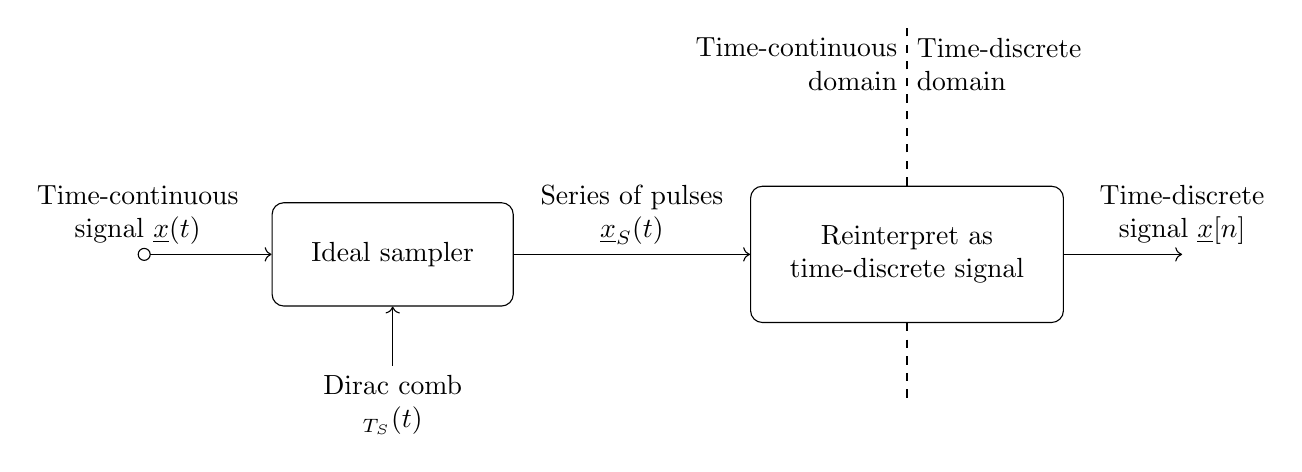
\begin{tikzpicture}
			\node[draw, block] (Sampler) {Ideal sampler};
			\node[draw, block, right=3cm of Sampler] (ReInterp) {Reinterpret as\\ time-discrete signal};
			
			\draw[<-o] (Sampler.west) -- ++(-1.7cm, 0) node[above, align=center]{Time-continuous\\ signal $\underline{x}(t)$};
			\draw[->] (Sampler.east) -- (ReInterp.west) node[midway, above, align=center]{Series of pulses\\ $\underline{x}_S(t)$};
			\draw[<-] (Sampler.south) -- ++(0, -0.75cm) node[below, align=center]{Dirac comb\\ $\Sha_{T_S}(t)$};
			\draw[->] (ReInterp.east) -- ++(1.5cm, 0) node[above, align=center]{Time-discrete\\ signal $\underline{x}[n]$};
			
			\draw[dashed] (ReInterp.north) -- ++(0, 2cm) node[below left, align=right]{Time-continuous\\ domain} node[below right, align=left]{Time-discrete\\ domain};
			\draw[dashed] (ReInterp.south) -- ++(0, -1cm);
		\end{tikzpicture}
	\end{adjustbox}
	\caption{An abstract view on sampling}
\end{figure}

\begin{excursus}{Normalisation of the sampled signal}
	\label{ref:ch04:normalization_xs}
	
	You may wonder about the equation \eqref{eq:ch04:sample_value}. Where does the $T_S$ in $T_S \underline{x}_S\left(n T_S\right)$ come from?
	
	\vspace{0.5em}
	
	The value of the sampled signal $\underline{x}_S\left(n T_S\right)$ is normalized by $\frac{1}{T_S}$. This is a result of the normalization of the Dirac delta function. Its argument shall be unitless. However, its argument $t - n T_S$ is a time unit. Consequently, the argument must be normalized by $T_S$.
	\begin{equation}
		\delta\left(t - n T_S\right) = \frac{1}{T_S} \delta\left(\frac{t}{T_S} - n\right)
	\end{equation}
	using the scaling property of the Dirac delta function, which is:
	\begin{equation}
		\delta\left(t\right) = \frac{1}{|a|} \left(\frac{t}{a}\right)
	\end{equation}
	\eqref{eq:ch04:ideal_sampling} can be rewritten to
	\begin{equation}
		\begin{split}
			\underline{x}_S(t) &= \sum\limits_{n = -\infty}^{\infty} \underline{x}\left(n T_S\right) \delta\left(t - n T_S\right) \\
			 &= \sum\limits_{n = -\infty}^{\infty} \underline{x}\left(n T_S\right) \cdot \frac{1}{T_S} \delta\left(\frac{t}{T_S} - n\right) \\
			T_S \underline{x}_S(t) &= \sum\limits_{n = -\infty}^{\infty} \underline{x}\left(n T_S\right) \delta\left(\frac{t}{T_S} - n\right) \\
		\end{split}
	\end{equation}
	The reason why $\underline{x}_S(t)$ needs to be normalized is, that it is an indefinitely small Dirac delta pulse. $T_S$ is the equidistant spacing between the pulses. $\frac{t}{T_S}$ guarantees a normalized spacing of $1$ between the samples.
	
	\vspace{0.5em}
	
	Why is $\underline{x}[n]$ not scaled? It is, but its normalization constant is not explicitly written. The equidistant spacing between $\underline{x}[n]$ and $\underline{x}[n+1]$ is $1$. Thus, their normalization constant is $1$, too.
	\begin{equation*}
		1 \cdot \underline{x}[n] = T_S \underline{x}_S\left(n T_S\right) = \underline{x}\left(n T_S\right)
	\end{equation*}
\end{excursus}

\subsubsection{Irreversibility of Sampling}

\begin{fact}
	The act of sampling is irreversible.
\end{fact}
	
There is a way to obtain the sampled signal:
\begin{equation*}
	\underline{x}_S(t) = \mathrm{Sampling} \left(\underline{x}(t)\right)
\end{equation*}
But there is generally no way back to reconstruct the original signal. $\mathrm{Sampling}^{-1} \left(\underline{x}_S(t)\right)$ does not exist.
\begin{equation*}
	\underline{x}(t) \neq \underbrace{\mathrm{Sampling}^{-1}}_{\text{Does not exist}} \left(\underline{x}_S(t)\right)
\end{equation*}

Sampling is always lossy in general.

\subsection{Sampling Theorem, Aliasing and Reconstruction}

\subsubsection{Frequency Domain Representation}

\begin{excursus}{Fourier transform of the Dirac comb}
	The Fourier transform of the Dirac comb is again a Dirac comb:
	\begin{equation}
		\begin{split}
			\Sha_{T}(t) \TransformHoriz \mathcal{F}\left\{\Sha_{T}(t)\right\} &= \frac{2 \pi}{T} \Sha_{\frac{2 \pi}{T}}(\omega) \\
			 &= \frac{2 \pi}{T} \sum\limits_{k = -\infty}^{\infty} \delta\left(\omega - k \frac{2 \pi}{T}\right) \\
			 &= \sum\limits_{k = -\infty}^{\infty} e^{- j \omega k T}
		\end{split}
		\label{eq:ch04:dirac_comb_fourier_tranform}
	\end{equation}
\end{excursus}

\eqref{eq:ch04:ideal_sampling} pointed out, that the sampled signal $\underline{x}_S(t)$ is the multiplication of the original time-domain signal $\underline{x}(t)$ and the Dirac comb $\Sha_{T_S}(t)$ with a periodicity of the sampling period $T_S$.
\begin{equation}
	\begin{split}
		\underline{x}_S(t) &= \underline{x}(t) \cdot \Sha_{T_S}(t) \\
		 &= \underline{x}(t) \cdot \frac{1}{T_S} \sum\limits_{n = -\infty}^{\infty} e^{j n \frac{2 \pi}{T_S} t} \\
		 &= \frac{1}{T_S} \sum\limits_{n = -\infty}^{\infty} \underbrace{\underline{x}(t) e^{j n \frac{2 \pi}{T_S} t}}_{\text{Frequency shift by } n \frac{2 \pi}{T_S}} \\
	\end{split}
\end{equation}

\textit{Remark:} Please note the normalization of the sampled signal by $T_S$, as explained on page \pageref{ref:ch04:normalization_xs}.

The ideally sampled signal $\underline{x}_S(t)$ can be expressed as a sum of \emph{frequency shifts} of the original signal $\underline{x}(t)$. Its Fourier transform is:
\begin{equation}
	\begin{split}
		\underline{X}_S\left(j \omega\right) &= \mathcal{F}\left\{\frac{1}{T_S} \sum\limits_{k = -\infty}^{\infty} \underline{x}(t) e^{j k \frac{2 \pi}{T_S} t}\right\} \\
		 & \qquad \text{Using the linearity of the Fourier transform:} \\
		 &= \frac{1}{T_S} \sum\limits_{k = -\infty}^{\infty} \mathcal{F}\left\{\underline{x}(t) e^{j k \frac{2 \pi}{T_S} t}\right\} \\
		 & \qquad \text{Using the frequency shift theorem of the Fourier transform:} \\
		 &= \frac{1}{T_S} \sum\limits_{k = -\infty}^{\infty} \underline{X}\left(j \left(\omega - k \frac{2 \pi}{T_S} \right)\right)
	\end{split}
\end{equation}

\textit{Remark:} Please note the normalization of the sampled signal by $T_S$, as explained on page \pageref{ref:ch04:normalization_xs}.

\begin{proof}{}
	An alternative way is using the Fourier transform of this multiplication in the time-domain is a convolution in the frequency domain:
	\begin{equation}
		\begin{split}
			\underline{X}_S\left(j \omega\right) &= \mathcal{F}\left\{\underline{x}(t) \cdot \Sha_{T_S}(t)\right\} \\
			 &= \frac{1}{2 \pi} \underline{X}\left(j \omega\right) * \left(\frac{2 \pi}{T_S} \Sha_{\frac{2 \pi}{T_S}}(\omega)\right) \\
			 &= \frac{1}{T_S} \int\limits_{-\infty}^{\infty} \underline{X}\left(j \left(\omega - \zeta\right)\right) \Sha_{\frac{2 \pi}{T_S}}\left(\zeta\right) \, \mathrm{d} \zeta \\
			 &= \frac{1}{T_S} \int\limits_{-\infty}^{\infty} \underline{X}\left(j \left(\omega - \zeta\right)\right) \sum\limits_{k = -\infty}^{\infty} \delta\left(\zeta - k \frac{2 \pi}{T_S}\right) \, \mathrm{d} \zeta \\
			 &= \frac{1}{T_S} \sum\limits_{k = -\infty}^{\infty} \int\limits_{-\infty}^{\infty} \underline{X}\left(j \left(\omega - \zeta\right)\right) \delta\left(\zeta - k \frac{2 \pi}{T_S}\right) \, \mathrm{d} \zeta \\
			 & \qquad \text{Using the Dirac measure:} \\
			 &= \frac{1}{T_S} \sum\limits_{k = -\infty}^{\infty} \underline{X}\left(j \left(\omega - k \frac{2 \pi}{T_S}\right)\right) \\
		\end{split}
	\end{equation}
\end{proof}

\textbf{Conclusion:} The spectrum of the sampled signal $\underline{X}_S\left(j \omega\right)$
\begin{itemize}
	\item consists of superimposed, frequency-shifted copies of the spectra of the original signal $\underline{X}\left(j\omega\right)$ and
	\item the periodicity of the superimposed, frequency-shifted copies is the sampling angular frequency $\omega_S = \frac{2 \pi}{T_S}$ or sampling frequency $f_S$, respectively,
	\item each frequency-shifted copy starts at $k \omega_S - \frac{\omega_S}{2}$ and ends at $k \omega_S + \frac{\omega_S}{2}$.
\end{itemize}

\begin{figure}[H]
	\subfloat[Original signal $\underline{X}\left(j\omega\right)$] {
		\centering
		\begin{tikzpicture}
				\begin{axis}[
				height={0.15\textheight},
				width=0.9\linewidth,
				scale only axis,
				xlabel={$\omega$},
				ylabel={$|\underline{X}\left(j\omega\right)|$},
				%grid style={line width=.6pt, color=lightgray},
				%grid=both,
				grid=none,
				legend pos=north east,
				axis y line=middle,
				axis x line=middle,
				every axis x label/.style={
					at={(ticklabel* cs:1.05)},
					anchor=north,
				},
				every axis y label/.style={
					at={(ticklabel* cs:1.05)},
					anchor=east,
				},
				xmin=-3.5,
				xmax=3.5,
				ymin=0,
				ymax=1.2,
				xtick={-1, -0.5, 0, 0.5, 1},
				xticklabels={$- \omega_S$, $- \frac{\omega_S}{2}$, $0$, $\frac{\omega_S}{2}$, $\omega_S$},
				ytick={0},
			]
				\draw[green, thick] (axis cs:-0.4,0) -- (axis cs:0,0.7);
				\draw[red, thick] (axis cs:0,0.7) -- (axis cs:0.4,0);
			\end{axis}
		\end{tikzpicture}
	}

	\subfloat[Spectrum of the Dirac comb $\frac{2 \pi}{T} \Sha_{\frac{2 \pi}{T}}(\omega)$] {
		\centering
		\begin{tikzpicture}
			\begin{axis}[
				height={0.15\textheight},
				width=0.9\linewidth,
				scale only axis,
				xlabel={$\omega$},
				ylabel={$|\frac{2 \pi}{T} \Sha_{\frac{2 \pi}{T}}(\omega)|$},
				%grid style={line width=.6pt, color=lightgray},
				%grid=both,
				grid=none,
				legend pos=north east,
				axis y line=middle,
				axis x line=middle,
				every axis x label/.style={
					at={(ticklabel* cs:1.05)},
					anchor=north,
				},
				every axis y label/.style={
					at={(ticklabel* cs:1.05)},
					anchor=east,
				},
				xmin=-3.5,
				xmax=3.5,
				ymin=0,
				ymax=1.2,
				xtick={-3, -2, ..., 3},
				xticklabels={$-3 \omega_S$, $-2 \omega_S$, $- \omega_S$, $0$, $\omega_S$, $2 \omega_S$, $3 \omega_S$},
				ytick={0},
			]
				\pgfplotsinvokeforeach{-3, -2, ..., 3}{
					\draw[-latex, blue, very thick] (axis cs:#1,0) -- (axis cs:#1,1);
				}
			\end{axis}
		\end{tikzpicture}
	}

	\subfloat[Sampled signal $\underline{X}_S\left(j\omega\right)$] {
	\centering
	\begin{tikzpicture}
		\begin{axis}[
			height={0.15\textheight},
			width=0.9\linewidth,
			scale only axis,
			xlabel={$\omega$},
			ylabel={$|\underline{X}_S\left(j\omega\right)|$},
			%grid style={line width=.6pt, color=lightgray},
			%grid=both,
			grid=none,
			legend pos=north east,
			axis y line=middle,
			axis x line=middle,
			every axis x label/.style={
				at={(ticklabel* cs:1.05)},
				anchor=north,
			},
			every axis y label/.style={
				at={(ticklabel* cs:1.05)},
				anchor=east,
			},
			xmin=-3.5,
			xmax=3.5,
			ymin=0,
			ymax=1.2,
			xtick={-3, -2, -1, -0.5, 0, 0.5, 1, 2, 3},
			xticklabels={$-3 \omega_S$, $-2 \omega_S$, $- \omega_S$, $- \frac{\omega_S}{2}$, $0$, $\frac{\omega_S}{2}$, $\omega_S$, $2 \omega_S$, $3 \omega_S$},
			ytick={0},
		]
			\pgfplotsinvokeforeach{-3, -2, ..., 3}{
				\draw[-latex, blue, dashed, very thick] (axis cs:#1,0) -- (axis cs:#1,1);
				\draw[green, thick] (axis cs:{#1-0.4},0) -- (axis cs:#1,0.7);
				\draw[red, thick] (axis cs:#1,0.7) -- (axis cs:{#1+0.4},0);
			}
		\end{axis}
	\end{tikzpicture}
	}

	\caption{Spectrum of the sampled signal}
\end{figure}

\begin{attention}
	The spectrum of the original signal $\underline{X}\left(j\omega\right)$ has both negative and positive frequencies. Remember that the symmetry rules apply \underline{only} for real-valued time-domain signals.
\end{attention}

\subsubsection{Aliasing}

The original signal in the previous example was limited to $- \frac{\omega_S}{2} \leq \omega \leq \frac{\omega_S}{2}$. The spectrum sampled signal consists of the frequency-shifted copies of the original signal's spectrum. Although they are superimposed, they do not overlap.

A problem arises when the original signal is \underline{not} limited to $- \frac{\omega_S}{2} \leq \omega \leq \frac{\omega_S}{2}$. The original signal's spectrum will overlap.

\begin{figure}[H]
	\subfloat[Original signal $\underline{X}\left(j\omega\right)$ violating the band-limitation $- \frac{\omega_S}{2} \leq \omega \leq \frac{\omega_S}{2}$. The original signal's spectrum will overlap.
	] {
		\centering
		\begin{tikzpicture}
			\begin{axis}[
				height={0.15\textheight},
				width=0.9\linewidth,
				scale only axis,
				xlabel={$\omega$},
				ylabel={$|\underline{X}\left(j\omega\right)|$},
				%grid style={line width=.6pt, color=lightgray},
				%grid=both,
				grid=none,
				legend pos=north east,
				axis y line=middle,
				axis x line=middle,
				every axis x label/.style={
					at={(ticklabel* cs:1.05)},
					anchor=north,
				},
				every axis y label/.style={
					at={(ticklabel* cs:1.05)},
					anchor=east,
				},
				xmin=-3.5,
				xmax=3.5,
				ymin=0,
				ymax=1.2,
				xtick={-3, -2, -1, -0.5, 0, 0.5, 1, 2, 3},
				xticklabels={$-3 \omega_S$, $-2 \omega_S$, $- \omega_S$, $- \frac{\omega_S}{2}$, $0$, $\frac{\omega_S}{2}$, $\omega_S$, $2 \omega_S$, $3 \omega_S$},
				ytick={0},
			]
				\draw[green, thick] (axis cs:-0.7,0) -- (axis cs:0,0.7);
				\draw[red, thick] (axis cs:0,0.7) -- (axis cs:0.8,0);
				\draw[olive, thick] (axis cs:2.1,0) -- (axis cs:2.1,0.5) -- (axis cs:2.3,0.5) -- (axis cs:2.3,0);
			\end{axis}
		\end{tikzpicture}
	}
	
	\subfloat[Spectrum of the Dirac comb $\frac{2 \pi}{T} \Sha_{\frac{2 \pi}{T}}(\omega)$] {
		\centering
		\begin{tikzpicture}
		\begin{axis}[
		height={0.15\textheight},
		width=0.9\linewidth,
		scale only axis,
		xlabel={$t$},
		ylabel={$|\frac{2 \pi}{T} \Sha_{\frac{2 \pi}{T}}(\omega)|$},
		%grid style={line width=.6pt, color=lightgray},
		%grid=both,
		grid=none,
		legend pos=north east,
		axis y line=middle,
		axis x line=middle,
		every axis x label/.style={
			at={(ticklabel* cs:1.05)},
			anchor=north,
		},
		every axis y label/.style={
			at={(ticklabel* cs:1.05)},
			anchor=east,
		},
		xmin=-3.5,
		xmax=3.5,
		ymin=0,
		ymax=1.2,
		xtick={-3, -2, ..., 3},
		xticklabels={$-3 \omega_S$, $-2 \omega_S$, $- \omega_S$, $0$, $\omega_S$, $2 \omega_S$, $3 \omega_S$},
		ytick={0},
		]
		\pgfplotsinvokeforeach{-3, -2, ..., 3}{
			\draw[-latex, blue, very thick] (axis cs:#1,0) -- (axis cs:#1,1);
		}
		\end{axis}
		\end{tikzpicture}
	}
	
	\subfloat[Sampled signal $\underline{X}_S\left(j\omega\right)$ showing aliasing] {
		\centering
		\begin{tikzpicture}
		\begin{axis}[
		height={0.15\textheight},
		width=0.9\linewidth,
		scale only axis,
		xlabel={$\omega$},
		ylabel={$|\underline{X}_S\left(j\omega\right)|$},
		%grid style={line width=.6pt, color=lightgray},
		%grid=both,
		grid=none,
		legend pos=north east,
		axis y line=middle,
		axis x line=middle,
		every axis x label/.style={
			at={(ticklabel* cs:1.05)},
			anchor=north,
		},
		every axis y label/.style={
			at={(ticklabel* cs:1.05)},
			anchor=east,
		},
		xmin=-3.5,
		xmax=3.5,
		ymin=0,
		ymax=1.2,
		xtick={-3, -2, -1, -0.5, 0, 0.5, 1, 2, 3},
		xticklabels={$-3 \omega_S$, $-2 \omega_S$, $- \omega_S$, $- \frac{\omega_S}{2}$, $0$, $\frac{\omega_S}{2}$, $\omega_S$, $2 \omega_S$, $3 \omega_S$},
		ytick={0},
		]
		\pgfplotsinvokeforeach{-3, -2, ..., 3}{
			\draw[-latex, blue, dashed, very thick] (axis cs:#1,0) -- (axis cs:#1,1);
			\draw[green, thick] (axis cs:{#1-0.7},0) -- (axis cs:#1,0.7);
			\draw[red, thick] (axis cs:#1,0.7) -- (axis cs:{#1+0.8},0);
			\draw[olive, thick] (axis cs:{#1+0.1},0) -- (axis cs:{#1+0.1},0.5) -- (axis cs:{#1+0.3},0.5) -- (axis cs:{#1+0.3},0);
		}
		\end{axis}
		\end{tikzpicture}
	}
	
	\caption{Aliasing}
\end{figure}

The sampled signal $\underline{X}_S\left(j\omega\right)$ contains overlapping, frequency-shifted copies of the original signal's spectrum. This is not feasible for most applications.

\begin{definition}{Anti-aliasing filter}
	A signal $\underline{x}(t)$ must be band-limited by an \index{anti-aliasing filter} \textbf{anti-aliasing filter} to avoid aliasing. The anti-aliasing filter is a \ac{LPF} with the cut-off frequency $\omega_o = \frac{\omega_S}{2}$.
	
	\begin{figure}[H]
		\centering
		\begin{adjustbox}{scale=0.7}
			\begin{circuitikz}
				\node[draw, block] (Sampler) {Ideal sampler};
				\node[draw, block, right=3cm of Sampler] (ReInterp) {Reinterpret as\\ time-discrete signal};
				
				\draw[<-o] (Sampler.west) to[lowpass] ++(-2.5cm, 0) -- ++(-0.7cm,0) node[above, align=center]{Time-continuous\\ signal $\underline{x}(t)$};
				\draw[->] (Sampler.east) -- (ReInterp.west) node[midway, above, align=center]{Series of pulses\\ $\underline{x}_S(t)$};
				\draw[<-] (Sampler.south) -- ++(0, -0.75cm) node[below, align=center]{Dirac comb\\ $\Sha_{T_S}(t)$};
				\draw[->] (ReInterp.east) -- ++(1.5cm, 0) node[above, align=center]{Time-discrete\\ signal $\underline{x}[n]$};
				
				\draw[dashed] (ReInterp.north) -- ++(0, 2cm) node[below left, align=right]{Time-continuous\\ domain} node[below right, align=left]{Time-discrete\\ domain};
				\draw[dashed] (ReInterp.south) -- ++(0, -1cm);
			\end{circuitikz}
		\end{adjustbox}
		\caption{An abstract view on sampling, including the anti-aliasing filter}
	\end{figure}
\end{definition}

The anti-aliasing filter's cut-off frequency must be half of the sampling frequency, because its bandwidth $\omega_S$ or $f_S$, respectively, must be distributed equally over the negative and positive part of the frequency axis.

\subsubsection{Reconstruction}

\textit{Remark:} Due to aliasing, there is no inverse function $\mathrm{Sampling}^{-1} \left(\underline{x}_S(t)\right)$ reversing the sampling process.

However, the original signal $\underline{x}(t)$ can be reconstructed if it was band-limited to the sampling (angular) frequency $\omega_S$ or $f_S$, respectively, before sampling.

\begin{definition}{Shannon-Nyquist sampling theorem}
	According to the \index{Shannon-Nyquist sampling theorem} \textbf{Shannon-Nyquist sampling theorem}, the original signal $\underline{x}(t)$ can be reconstructed if the sample rate $T_S$ is at least twice the inverse of signal's highest (angular) frequency $\omega_B$ or $f_B$, respectively.
	\begin{equation}
		T_S \geq \frac{1}{2 f_B} = \frac{\pi}{\omega_B}
	\end{equation}
\end{definition}

The \index{reconstruction} \textbf{reconstruction} of a sampled signal is done by:
\begin{itemize}
	\item Reinterpreting the time-discrete signal $\underline{x}[n]$ again as a time-continuous, sampled signal $\underline{x}_S(t)$.
	\item Removing the copies of the original signal in the frequency domain, using a \ac{LPF} (\index{reconstruction filter} \textbf{reconstruction filter}) with the cut-off frequency $\omega_o = \frac{\omega_S}{2}$.
\end{itemize}

\begin{figure}[H]
	\centering
	\begin{adjustbox}{scale=0.7}
		\begin{circuitikz}
			\node[draw, block, right=3cm of Sampler] (ReInterp) {Reinterpret as\\ time-continuous signal};
			
			\draw[<-o] (ReInterp.west) -- ++(-1.5cm, 0) node[above, align=center]{Time-discrete\\ signal $\underline{x}[n]$};
			\draw (ReInterp.east) -- ++(3cm,0) node[midway, above, align=center]{Series of pulses\\ $\underline{x}_S(t)$}
				to[lowpass] ++(2.5cm,0 ) -- ++(0.7cm, 0) node[above, align=center]{Reconstructed\\ time-continuous\\ signal $\underline{\tilde{x}}(t)$};
			
			\draw[dashed] (ReInterp.north) -- ++(0, 2cm) node[below left, align=right]{Time-discrete\\ domain} node[below right, align=left]{Time-continuous\\ domain};
			\draw[dashed] (ReInterp.south) -- ++(0, -1cm);
		\end{circuitikz}
	\end{adjustbox}
	\caption{An abstract view on reconstruction}
\end{figure}

The reconstructed signal $\underline{\tilde{x}}(t)$ equals the original signal $\underline{x}(t)$ only if the Shannon-Nyquist theorem is fulfilled.
\begin{equation}
	\underline{\tilde{x}}(t) = \underline{x}(t) \qquad \text{if $\underline{x}(t)$ band-limtied to $-\frac{\omega_S}{2} \leq \omega \leq \frac{\omega_S}{2}$}
\end{equation}

\begin{figure}[H]
	
	\subfloat[Sampled signal $\underline{X}_S\left(j\omega\right)$] {
		\centering
		\begin{tikzpicture}
			\begin{axis}[
				height={0.15\textheight},
				width=0.9\linewidth,
				scale only axis,
				xlabel={$\omega$},
				ylabel={$|\underline{X}_S\left(j\omega\right)|$},
				%grid style={line width=.6pt, color=lightgray},
				%grid=both,
				grid=none,
				legend pos=north east,
				axis y line=middle,
				axis x line=middle,
				every axis x label/.style={
					at={(ticklabel* cs:1.05)},
					anchor=north,
				},
				every axis y label/.style={
					at={(ticklabel* cs:1.05)},
					anchor=east,
				},
				xmin=-3.5,
				xmax=3.5,
				ymin=0,
				ymax=1.2,
				xtick={-3, -2, -1, -0.5, 0, 0.5, 1, 2, 3},
				xticklabels={$-3 \omega_S$, $-2 \omega_S$, $- \omega_S$, $- \frac{\omega_S}{2}$, $0$, $\frac{\omega_S}{2}$, $\omega_S$, $2 \omega_S$, $3 \omega_S$},
				ytick={0},
			]
				\pgfplotsinvokeforeach{-3, -2, ..., 3}{
					\draw[-latex, blue, dashed, very thick] (axis cs:#1,0) -- (axis cs:#1,1);
					\draw[green, thick] (axis cs:{#1-0.4},0) -- (axis cs:#1,0.7);
					\draw[red, thick] (axis cs:#1,0.7) -- (axis cs:{#1+0.4},0);
				}
			
				\draw[black, thick, dashed] (axis cs:-0.5,0) -- (axis cs:-0.5,0.9) -- (axis cs:0.5,0.9) -- (axis cs:0.5,0);
				\draw (axis cs:0.3,0.9) -- (axis cs:0.4,1.0) node[above right, align=left]{Reconstruction filter};
			\end{axis}
		\end{tikzpicture}
	}

	\subfloat[Reconstructed signal $\underline{\tilde{X}}\left(j\omega\right)$] {
		\centering
		\begin{tikzpicture}
			\begin{axis}[
				height={0.15\textheight},
				width=0.9\linewidth,
				scale only axis,
				xlabel={$\omega$},
				ylabel={$|\underline{\tilde{X}}\left(j\omega\right)|$},
				%grid style={line width=.6pt, color=lightgray},
				%grid=both,
				grid=none,
				legend pos=north east,
				axis y line=middle,
				axis x line=middle,
				every axis x label/.style={
					at={(ticklabel* cs:1.05)},
					anchor=north,
				},
				every axis y label/.style={
					at={(ticklabel* cs:1.05)},
					anchor=east,
				},
				xmin=-3.5,
				xmax=3.5,
				ymin=0,
				ymax=1.2,
				xtick={-1, -0.5, 0, 0.5, 1},
				xticklabels={$- \omega_S$, $- \frac{\omega_S}{2}$, $0$, $\frac{\omega_S}{2}$, $\omega_S$},
				ytick={0},
			]
				\draw[green, thick] (axis cs:-0.4,0) -- (axis cs:0,0.7);
				\draw[red, thick] (axis cs:0,0.7) -- (axis cs:0.4,0);
			\end{axis}
		\end{tikzpicture}
	}
	
	\caption{Reconstruction of a sampled signal}
\end{figure}

\subsection{Discrete-Time Fourier Transform}

Using \eqref{eq:ch04:ideal_sampling} and \eqref{eq:ch04:sample_value}, a expression depending on the time-discrete signal $\underline{x}[n]$ can be formulated:
\begin{equation}
	\underline{x}_S(t) = \sum\limits_{n = -\infty}^{\infty} \underline{x}[n] \cdot \delta(t - n T_S)
\end{equation}

The Fourier transform of the sampled signal $\underline{x}_S(t)$ is:
\begin{equation}
	\begin{split}
		\underline{X}_S \left(j \omega\right) &= \mathcal{F} \left\{\underline{x}_S(t)\right\} \\
		 &= \mathcal{F} \left\{\sum\limits_{n = -\infty}^{\infty} \underline{x}[n] \cdot \delta(t - n T_S)\right\} \\
		 &= \int\limits_{t = -\infty}^{\infty} \sum\limits_{n = -\infty}^{\infty} \underline{x}[n] \cdot \delta(t - n T_S) \cdot e^{-j \omega t} \, \mathrm{d} t \\
		 &= \sum\limits_{n = -\infty}^{\infty} \underline{x}[n] \int\limits_{t = -\infty}^{\infty} \delta(t - n T_S) \cdot e^{-j \omega t} \, \mathrm{d} t \\
		 &\qquad \text{Using the Dirac measure:} \\
		 &= \underbrace{\sum\limits_{n = -\infty}^{\infty} \underline{x}[n] \cdot e^{-j \omega n T_S}}_{= \underline{X}_{\frac{2\pi}{T_S}} \left(e^{j T_S \omega}\right)}
	\end{split}
	\label{eq:ch04:sampled_signal_spectrum}
\end{equation}

Redefining $\phi = T_S \omega$:
\begin{equation}
	\underline{X}_S \left(j \omega\right) = \left.\underline{X}_{\frac{2\pi}{T_S}} \left(e^{j T_S \omega}\right)\right|_{T_S \omega = \phi} = \underline{X}_{2 \pi} \left(e^{j \phi}\right) = \sum\limits_{n = -\infty}^{\infty} \underline{x}[n] \cdot e^{-j \phi n}
\end{equation}

$\underline{X}_{2 \pi} \left(e^{j \phi}\right)$ or $\underline{X}_{\frac{2\pi}{T_S}} \left(e^{j T_S \omega}\right)$, respectively, is the discrete-time Fourier transform of the time-discrete, sampled signal $\underline{x}[n]$.
\begin{itemize}
	\item The spectrum of the sampled signal $\underline{X}_{\frac{2\pi}{T_S}} \left(e^{j T_S \omega}\right)$ is $\omega_S$-periodic or (with $\omega_S = \frac{2\pi}{T_S}$) $\frac{2\pi}{T_S}$-periodic.
	\item The $\frac{2\pi}{T_S}$-periodicity is equivalent to to a full $2\pi$-rotation on the unit circle $e^{j \phi}$ in the complex plane.
	\item The real-valued frequency-continuous variable $\omega$ is replaced by the complex-valued frequency-continuous variable $e^{j \phi}$ representing the periodicity of the spectrum.
	\item $\phi = T_S \omega$
	\item An alternate but equivalent expression $\underline{X}_{2 \pi} \left(e^{j \phi}\right)$ uses the $2\pi$-periodicity.
\end{itemize}

Both $\underline{X}_{2 \pi} \left(e^{j \phi}\right)$ and $\underline{X}_{\frac{2\pi}{T_S}} \left(e^{j T_S \omega}\right)$ are equivalent. However, they are normalized differently.
\begin{itemize}
	\item The spectrum of $\underline{X}_{\frac{2\pi}{T_S}} \left(e^{j T_S \omega}\right)$ is normalized to the sampling angular frequency $\frac{2 \pi}{T_S}$.
	\item The spectrum of $\underline{X}_{2 \pi} \left(e^{j \phi}\right)$ is normalized to the full rotation on the unit circle $2 \pi$.
\end{itemize}
The normalization is of minor importance for the \ac{DTFT}, but must be considered for the inverse \ac{DTFT}. Both $\underline{X}_{2 \pi} \left(e^{j \phi}\right)$ and $\underline{X}_{\frac{2\pi}{T_S}} \left(e^{j T_S \omega}\right)$ are complex-valued Fourier series (see \eqref{eq:ch04:sampled_signal_spectrum}). For $\underline{X}_{\frac{2\pi}{T_S}} \left(e^{j T_S \omega}\right)$, the normalization factor $\frac{T_S}{2 \pi}$ must be considered and, for $\underline{X}_{2 \pi} \left(e^{j \phi}\right)$, the normalization factor $\frac{1}{2 \pi}$.

\begin{definition}{Discrete-time Fourier transform}
	The \index{discrete-time Fourier transform} \textbf{\acf{DTFT}} of a time-discrete signal $\underline{x}[n]$ with the sampling period $T_S$ is:
	\begin{itemize}
		\item normalized to $\omega_S = \frac{2\pi}{T_S}$ ($\omega_S$-periodicity):
		\begin{equation}
			\underline{X}_{\frac{2\pi}{T_S}} \left(e^{j T_S \omega}\right) = \sum\limits_{n = -\infty}^{\infty} \underline{x}[n] \cdot e^{-j T_S \omega n}
		\end{equation}
		\item normalized to $2 \pi$ ($2 \pi$-periodicity):
		\begin{equation}
			\underline{X}_{2 \pi} \left(e^{j \phi}\right) = \sum\limits_{n = -\infty}^{\infty} \underline{x}[n] \cdot e^{-j \phi n}
		\end{equation}
	\end{itemize}
	Both expressions are equivalent ($\phi = T_S \omega$).
	
	The \index{discrete-time Fourier transform!inverse} \textbf{inverse discrete-time Fourier transform} is:
	\begin{itemize}
		\item normalized to $\omega_S = \frac{2\pi}{T_S}$ ($\omega_S$-periodicity):
		\begin{equation}
			\underline{x}[n] = \frac{T_S}{2 \pi} \int\limits_{- \frac{\pi}{T_S}}^{+ \frac{\pi}{T_S}} \underline{X}_{\frac{2\pi}{T_S}}(e^{j T_S \omega}) \cdot e^{+ j \omega T_S n} \, \mathrm{d} \omega
		\end{equation}
		\item normalized to $2 \pi$ ($2 \pi$-periodicity):
		\begin{equation}
			\underline{x}[n] = \frac{1}{2 \pi} \int\limits_{- \pi}^{+ \pi} \underline{X}_{2\pi}(e^{j \phi}) \cdot e^{+ j \phi n} \, \mathrm{d} \phi
		\end{equation}
	\end{itemize}
	Both expressions are equivalent.
\end{definition}

\subsubsection{Properties}

The \ac{DTFT} is derived from the \ac{CTFT}. Therefore, all properties apply likewise.
\begin{itemize}
	\item Linearity
	\item Time shift, frequency shift
	\item Convolution theorem
	\item Duality
	\item Symmetry rules
\end{itemize}

\subsection{z-Transform}

Analogous to the Fourier and Laplace transform, the \acf{DTFT} is a special case of the z-transform.

\begin{definition}{z-transform}
	The \index{z-transform} \textbf{z-transform} of a time-discrete signal $\underline{x}[n]$ with the sampling period $T_S$ is:
	\begin{equation}
		\underline{X}\left(\underline{z}\right) = \mathcal{Z}\left\{\underline{x}[n]\right\} = \sum\limits_{n = -\infty}^{\infty} \underline{x}[n] \cdot \underline{z}^{-n}
	\end{equation}
	$\underline{z}$ is the complex frequency variable.
	
	The  \index{z-transform!inverse} \textbf{inverse z-transform} is:
	\begin{equation}
		\underline{x}[n] = \mathcal{Z}^{-1}\left\{\underline{x}[n]\right\} = \frac{1}{2 \pi j} \oint\limits_{C} \underline{X}\left(\underline{z}\right) \underline{z}^{n-1} \, \mathrm{d} \underline{z}
	\end{equation}
	$C$ is a counter-clockwise closed path enclosing the origin and the region of convergence. In the case of the \ac{DTFT}, $C$ is the unit circle, i.e., $C = [e^{-j \pi}, e^{j \pi}]$.
\end{definition}

$\underline{z}$ can be decomposed into:
\begin{equation}
	\underline{z} = A e^{j \phi}
\end{equation}
where $A$ represents the gain and $e^{j \phi}$ the frequency.
\begin{figure}[H]
	\centering
	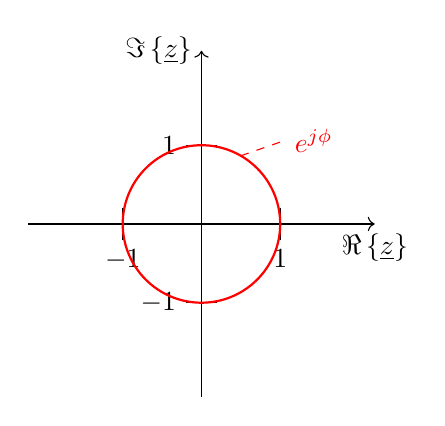
\begin{tikzpicture}
		\draw[->] (-2.2,0) -- (2.2,0) node[below, align=left]{$\Re\left\{\underline{z}\right\}$};
		\draw[->] (0,-2.2) -- (0,2.2) node[left, align=right]{$\Im\left\{\underline{z}\right\}$};
		%\draw (0:1) arc(0:360:1);
		\draw (1,0.2) -- (1,-0.2) node[below]{$1$};
		\draw (-1,0.2) -- (-1,-0.2) node[below]{$-1$};
		\draw (0.2,1) -- (-0.2,1) node[left]{$1$};
		\draw (0.2,-1) -- (-0.2,-1) node[left]{$-1$};
		
		\draw[thick, red] (0:1) arc(0:360:1);
		\draw[dashed, red] (60:1) -- (45:1.5) node[right, align=left, color=red]{$e^{j \phi}$};
	\end{tikzpicture}
	\caption{Complex plane of the complex frequency variable $\underline{z}$}
	\label{fig:ch04:ztrafo_z_cmplx_plane}
\end{figure}

In the \acf{DTFT}, $A = 1$ as a special case. The remainig $e^{j \phi}$ describes the unit circle in the complex plane. Like the Fourier transform, it assumes a steady-state, whereas the z-transform delivers a complete description of a time-discrete system. The z-transform is preferred for transient analysis of a time-discrete system. Its zeros $\underline{z}_0$ and poles $\underline{z}_\infty$ determine the stability of the system.

Figure \ref{fig:ch04:ztrafo_z_cmplx_plane} makes evident the $2 \pi$-periodicity of both the \ac{DTFT} and z-transform. The frequency $e^{j \phi}$ repeats every $2 \pi$.

\subsection{Discrete Fourier Transform}

\subsubsection{Periodic Sequences}

Given is an $N$-periodic sequence of samples $\underline{x}_p[n]$:
\begin{equation}
	\underline{x}_p[n] = \underline{x}_p[n + mN] \qquad \forall \; m \in \mathbb{Z}
\end{equation}

A corollary of the periodicity is that the \ac{DTFT} $\underline{X}_{2 \pi} \left(e^{j \phi}\right)$ or $\underline{X}_{\frac{2\pi}{T_S}} \left(e^{j T_S \omega}\right)$, respectively, is not only periodic. It is zero for
\begin{itemize}
	\item $\underline{X}_{2 \pi} \left(e^{j \phi}\right) = 0$ for $\phi \neq m \frac{2\pi}{N}$ where $m \in \mathbb{Z}$, or
	\item $\underline{X}_{\frac{2\pi}{T_S}} \left(e^{j T_S \omega}\right) = 0$ for $\omega \neq m \frac{2\pi}{T_S N}$ where $m \in \mathbb{Z}$.
\end{itemize}
The \ac{DTFT} itself becomes a series of pulses (Dirac comb) with an equidistant spacing of
\begin{itemize}
	\item $\frac{2\pi}{N}$ for $\underline{X}_{2 \pi} \left(e^{j \phi}\right)$, or
	\item $\frac{2\pi}{T_S N}$ for $\underline{X}_{\frac{2\pi}{T_S}} \left(e^{j T_S \omega}\right)$, respectively.
\end{itemize}

This can be explained using the duality of the \ac{DTFT}:
\begin{figure}[H]
	\centering
	\begin{adjustbox}{scale=0.75}
		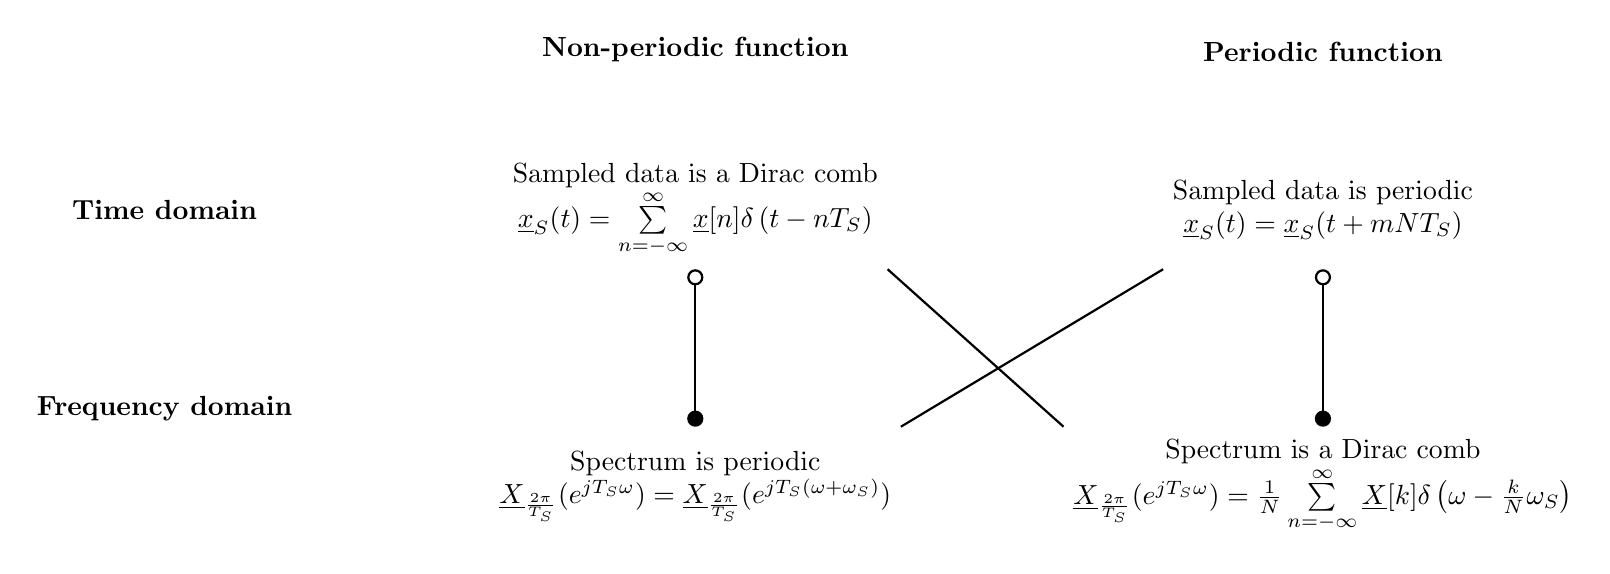
\begin{tikzpicture}
			\node[align=center, minimum width=2.5cm, minimum height=1.5cm] (TD1) {Sampled data is a Dirac comb\\ $\underline{x}_S(t) = \sum\limits_{n = -\infty}^{\infty} \underline{x}[n] \delta\left(t - n T_S\right)$};
			\node[align=center, minimum width=2.5cm, minimum height=1.5cm, right=3.5cm of TD1] (TD2) {Sampled data is periodic\\ $\underline{x}_S(t) = \underline{x}_S(t + m N {T_S})$};
			\node[align=center, minimum width=2.5cm, minimum height=1.5cm, below=2cm of TD1] (FD1) {Spectrum is periodic\\ $\underline{X}_{\frac{2\pi}{T_S}}(e^{j T_S \omega}) = \underline{X}_{\frac{2\pi}{T_S}}(e^{j T_S \left(\omega + \omega_S\right)})$};
			\node[align=center, minimum width=2.5cm, minimum height=1.5cm, below=2cm of TD2] (FD2) {Spectrum is a Dirac comb\\ $\underline{X}_{\frac{2\pi}{T_S}}(e^{j T_S \omega}) = \frac{1}{N} \sum\limits_{n = -\infty}^{\infty} \underline{X}[k] \delta\left(\omega - \frac{k}{N} \omega_S\right)$};
			
			\node[align=right, anchor=east, left=3cm of TD1] (LabelTD) {\textbf{Time domain}};
			\node[align=right, anchor=east, below=2cm of LabelTD] (LabelFD) {\textbf{Frequency domain}};
			\node[align=right, above=1cm of TD1] (Func1) {\textbf{Non-periodic function}};
			\node[align=right, above=1cm of TD2] (Func2) {\textbf{Periodic function}};
			
			%\draw (TD1) node[midway, align=right, rotate=-90]{$\TransformHoriz$} (FD1);
			%\draw (TD2) node[midway, align=right, rotate=-90]{$\TransformHoriz$} (FD2);
			\draw[o-*, thick] (TD1.south) -- (FD1.north);
			\draw[o-*, thick] (TD2.south) -- (FD2.north);
			
			\draw[thick] (TD1.south east) -- (FD2.north west);
			\draw[thick] (TD2.south west) -- (FD1.north east);
		\end{tikzpicture}
	\end{adjustbox}
	\caption{Due to the duality, the \ac{DTFT} of a periodic signal is series of pulses (Dirac comb).}
\end{figure}

The \ac{DTFT} of a periodic signal is still periodic. The maximum number of unique, discrete frequency samples in the \ac{DTFT} is
\begin{equation}
	\frac{\text{Periodicity of the \ac{DTFT}}}{\text{Spacing between the pulses}} = \frac{\frac{2\pi}{T_S}}{\frac{2\pi}{T_S N}} = N
\end{equation}

Because of the periodicity of both the time-domain and frequency-domain signal, the signal is fully determined by either
\begin{itemize}
	\item $N$ samples in the time domain, or
	\item $N$ samples in the frequency domain.
\end{itemize}

The samples in the frequency domain are
\begin{equation}
	\underline{X}[k] = \left.\underline{X}_{2 \pi} \left(e^{j \phi}\right)\right|_{\phi = k \frac{2\pi}{N}} = \left.\underline{X}_{\frac{2\pi}{T_S}} \left(e^{j T_S \omega}\right)\right|_{\omega = k \frac{2\pi}{T_S N}} = \sum\limits_{n = 0}^{N-1} \underline{x}[n] e^{-j 2\pi \frac{k}{N} n}
\end{equation}
where $k \in \mathbb{Z}$ is the discrete frequency variable. The summation boundaries $[0, N-1]$ can be replaced by any sequence of length $N$, because $\underline{x}[n]$ is $N$-periodic.

$\underline{X}[k]$ is the \ac{DFT}. $\underline{X}[k]$ is $N$-periodic.

The \ac{DTFT} is obtained by:
\begin{equation}
	\underline{X}_{\frac{2\pi}{T_S}} \left(e^{j T_S \omega}\right) = \frac{2\pi}{N T_S} \sum\limits_{k = -\infty}^{\infty} \underline{X}[k] \cdot \delta\left(\omega - \frac{k}{N} \underbrace{\frac{2\pi}{T_S}}_{= \omega_S}\right)
\end{equation}

\textit{Remark:} $\omega$ is normalized to $\frac{N T_S}{2\pi}$. Accordingly, the sum is normalized to $\frac{2\pi}{N T_S}$. Considerations analogous to the explanation on page \pageref{ref:ch04:normalization_xs} apply.

The inverse \ac{DTFT} is:
\begin{equation}
	\begin{split}
		\underline{x}[n] &= \frac{T_S}{2 \pi} \int\limits_{- \frac{\pi}{T_S}}^{+ \frac{\pi}{T_S}} \frac{2\pi}{N T_S} \sum\limits_{k = -\infty}^{\infty} \underline{X}[k] \cdot \delta\left(\omega - \frac{k}{N} \frac{2\pi}{T_S}\right) \cdot e^{+ j \omega T_S n} \, \mathrm{d} \omega \\
		 &\qquad \text{Integration boundaries propagate to summation boundaries via $\omega - \frac{k}{N} \frac{2\pi}{T_S} \stackrel{!}{=} 0$:} \\
		 &= \frac{1}{N} \sum\limits_{k = -\frac{N}{2}}^{\frac{N}{2}} \underline{X}[k] \cdot \int\limits_{- \frac{\pi}{T_S}}^{+ \frac{\pi}{T_S}} \delta\left(\omega - \frac{k}{N} \frac{2\pi}{T_S}\right) \cdot e^{+ j \omega T_S n} \, \mathrm{d} \omega \\
		 &\qquad \text{Using the Dirac measure:} \\
		 &= \frac{1}{N} \sum\limits_{k = -\frac{N}{2}}^{\frac{N}{2}} \underline{X}[k] \cdot e^{+ j 2\pi \frac{k}{N} n}
	\end{split}
\end{equation}
This is the inverse \ac{DFT}. Again the summation boundaries of $[-\frac{N}{2}, \frac{N}{2}]$ can be replaced by any sequence of length $N$, because $\underline{X}[k]$ is $N$-periodic.

\begin{definition}{Discrete Fourier transform}
	The \index{discrete Fourier transform} \textbf{\acf{DFT}} of a $N$-periodic sequence $\underline{x}[n]$ is:
	\begin{equation}
		\underline{X}[k] = \mathcal{F}_{\text{DFT}}\left\{\underline{x}[n]\right\} = \sum\limits_{n \in N} \underline{x}[n] \cdot e^{-j 2\pi \frac{k}{N} n}
		\label{eq:ch04:dft}
	\end{equation}
	
	The \index{inverse discrete Fourier transform} \textbf{inverse discrete Fourier transform} is:
	\begin{equation}
		\underline{x}[n] = \mathcal{F}_{\text{DFT}}^{-1}\left\{\underline{X}[k]\right\} = \frac{1}{N} \sum\limits_{k \in N} \underline{X}[k] \cdot e^{+ j 2\pi \frac{k}{N} n}
		\label{eq:ch04:idft}
	\end{equation}
	
	Both $\underline{X}[k]$ and $\underline{x}[n]$ are $N$-periodic. The summation boundaries can be chosen to any sequence of length $N$.
\end{definition}

\subsubsection{Properties}

The \ac{DFT} is derived from the \ac{DTFT} and \ac{CTFT}. Therefore, all properties apply likewise.
\begin{itemize}
	\item Linearity
	\item Time shift, frequency shift
	\item Convolution theorem
	\item Duality
	\item Symmetry rules
\end{itemize}

\subsection{Orthogonality of the \acs{DFT} Frequency Vectors}

Both the time-domain sequence $\underline{x}[n]$ and frequency-domain sequence $\underline{X}[k]$ can be interpreted as vectors:
\begin{itemize}
	\item $\cmplxvect{x} = \left[\underline{x}[0], \underline{x}[1], \dots, \underline{x}[N-1]\right]^{\mathrm{T}}$
	\item $\cmplxvect{X} = \left[\underline{X}[0], \underline{X}[1], \dots, \underline{X}[N-1]\right]^{\mathrm{T}}$
\end{itemize}

The \ac{DFT} \eqref{eq:ch04:dft} can be expressed as a linear system of equation:
\begin{equation}
	\cmplxvect{X} = \underline{\mat{F}} \cdot \cmplxvect{x}
\end{equation}

The $N \times N$ transformation matrix $\underline{\mat{F}}$ is the \index{DFT matrx} \textbf{\ac{DFT} matrix} with the elements:
\begin{equation}
	\underline{F}_{pq} = \underline{w}^{p \cdot q}
\end{equation}
where $\underline{w}$ is the $N$-th \index{primitive root of unity} \textbf{primitive root of unity}\footnote{The primitive root of unity divide the unit circle $e^{j \phi}$ into equally sized segments.}.\nomenclature[Sw]{$\underline{w}_N$}{$N$-th primitive root of unity}
\begin{equation}
	\underline{w} = e^{j \frac{2 \pi}{N}}
\end{equation}
So
\begin{equation}
	\underline{\mat{F}} = \left[
	\begin{matrix}
		1 & 1 & 1 & 1 & \ldots & 1 \\
		1 & \underline{w} & \underline{w}^2 & \underline{w}^3 & \ldots & \underline{w}^{N-1} \\
		1 & \underline{w}^2 & \underline{w}^4 & \underline{w}^6 & \ldots & \underline{w}^{2\left(N-1\right)} \\
		1 & \underline{w}^3 & \underline{w}^6 & \underline{w}^9 & \ldots & \underline{w}^{3\left(N-1\right)} \\
		\vdots & \vdots & \vdots & \vdots & \ddots & \vdots \\
		1 & \underline{w}^{N-1} & \underline{w}^{2\left(N-1\right)} & \underline{w}^{3\left(N-1\right)} & \ldots & \underline{w}^{\left(N-1\right)\left(N-1\right)} \\
	\end{matrix}
	\right]
\end{equation}

The inverse \ac{DFT} is, using the conjugate complex $\overline{\underline{\mat{F}}}$:
\begin{equation}
	\cmplxvect{x} = \frac{1}{N} \overline{\underline{\mat{F}}} \cdot \cmplxvect{X}
\end{equation}

Each row and column of $\underline{\mat{F}}$ is a vector of powers of the $N$-th primitive root of unity $\underline{w}$. A row with the index $k$ is $\cmplxvect{u}_k$.
\begin{equation}
	\begin{split}
		\cmplxvect{u}_k &= \left[\left.\underline{w}^{k \cdot q}\right| q = 0, 1, \dots, N-1\right]^{\mathrm{T}} \\
		 &= \left[1, \underline{w}^{k}, \underline{w}^{2 k}, \underline{w}^{3 k}, \dots, \underline{w}^{k \left(N-1\right)} \right]^{\mathrm{T}} \\
		 &= \left[1, e^{j \frac{2 \pi}{N} k}, e^{j \frac{2 \pi}{N} 2 k}, e^{j \frac{2 \pi}{N} 3 k}, \dots, e^{j \frac{2 \pi}{N} k \left(N-1\right)} \right]^{\mathrm{T}} \\
	\end{split}
\end{equation}
Each vector $\cmplxvect{u}_k$ is the basis for the associated frequency sample $\underline{X}[k]$.

It can be shown that the vectors $\cmplxvect{u}_k$ are orthogonal. They form an \index{orthogonal basis} \textbf{orthogonal basis}. This can be proven by their inner product:
\begin{equation}
	\begin{split}
		\langle \cmplxvect{u}_p, \overline{\cmplxvect{u}_q} \rangle &= \sum\limits_{n=0}^{N-1} \left(e^{j \frac{2 \pi}{N} p n}\right) \overline{\left(e^{j \frac{2 \pi}{N} q n}\right)} \\
		 &= \sum\limits_{n=0}^{N-1} e^{j \frac{2 \pi}{N} \left(p - q\right) n} \\
		 &= N \delta_{pq}
	\end{split}
\end{equation}

\textit{Remark:} $\delta_{pq}$ is the Kronecker delta here.

\begin{itemize}
	\item The vectors $\cmplxvect{u}_p$ and $\cmplxvect{u}_q$ are orthogonal ($\delta_{pq} = 0$) for $p \neq q$.
	\item $\delta_{pq}$ is non-zero only if $p = q$.
\end{itemize}

\begin{fact}
	The basis of the frequency samples of a \ac{DFT} are orthogonal.
\end{fact}

\subsection{Processing of Non-Periodic Signals}

In practical digital systems, signals are non-periodic. A non-periodic sequence $\underline{x}[n]$ can be fully transformed by the \ac{DTFT}.
\begin{equation}
	\underline{x}[n] \TransformHoriz \mathcal{F}_{\text{DTFT}}\left\{\underline{x}[n]\right\} = \underline{X}_{\frac{2\pi}{T_S}}\left(e^{j T_S \omega}\right)
\end{equation}

However, it is not feasible to implement a \ac{DTFT}, because the sums and integrals run over an indefinite interval. Therefore, the transforms are approximated by the \ac{DFT}.

\subsubsection{Windowing and Periodic Continuation}

A sequence of length $N$ is taken out of $\underline{x}[n]$:
\begin{equation}
	\underline{\tilde{x}}_N[n] = \left[\underline{x}[m], \underline{x}[m+1], \underline{x}[m+1], \dots, \underline{x}[m+N-1]\right]
\end{equation}
The act of extracting $N$ subsequent samples out of $\underline{x}[n]$ is called \index{windowing} \textbf{windowing}. To illustrate this, imagine that you watch a sequence moving to the left through a window. The movement to the left is the time advance. Because of the window, you see a certain extract of $\underline{x}[n]$ only at one time.

%TODO
%\todo{Window illustration}

This sequence is repeated indefinitely (\emph{periodic continuation}):
\begin{equation}
	\underline{x}_N[n] = \underline{\tilde{x}}_N[n \mod N]
\end{equation}
Thus, $\underline{x}_N[n]$ is periodic:
\begin{equation}
	\underline{x}_N[n] = \underline{x}_N[n + q N] \qquad \forall \; q \in \mathbb{Z}
\end{equation}

Now, $\underline{x}_N[n]$ can be transformed to the frequency-domain using the \ac{DFT}.
\begin{equation}
	\underline{x}_N[n] \TransformHoriz \mathcal{F}_{\text{DFT}}\left\{\underline{x}[n]\right\} = \underline{X}[k]
\end{equation}

The periodic continuation is just a theoretical explanation. In practise, it is enough to calculate the \ac{DFT} over $N$ subsequent samples out of $\underline{x}[n]$.
\begin{equation}
	\begin{split}
		\underline{X}_{\frac{2\pi}{T_S}}\left(e^{j T_S \omega}\right) &\approx \begin{cases}
			\left.\underline{X}[k]\right|_{k = N \frac{T_S}{2\pi} \omega} & \quad \text{if } \left(N \frac{T_S}{2\pi} \omega\right) \in \mathbb{Z}, \\
			0 & \quad \text{if } \left(N \frac{T_S}{2\pi} \omega\right) \notin \mathbb{Z}.
		\end{cases} \\
		\underline{X}_{\frac{2\pi}{T_S}}\left(e^{j 2 \pi \frac{k}{N}}\right) &\approx \underline{X}[k] = \sum\limits_{n=0}^{N-1} \underline{x}_N[n] e^{-j 2 \pi \frac{k}{N} n}
	\end{split}
	\label{eq:ch04:dtft_sampling}
\end{equation}

Windowing and periodic continuation is, in fact, a sampling of the \ac{DTFT} (see \eqref{eq:ch04:dtft_sampling}).

\subsubsection{Window Functions}

The widowing of $\underline{x}[n]$ to obtain $\underline{x}_N[n]$ as discussed before did not change the values of $\underline{x}[n]$. This can be expressed as a multiplication of the original sequence with the rectangular function:
\begin{equation}
	\underline{x}_W[n] = \underline{x}_N[n] \cdot \underbrace{w_{rect,M}[n]}_{\text{Rectangular window}}
\end{equation}
where $w_{rect,M}[n]$ is the rectangular function of the length $M$:
\begin{equation}
	w_{rect,M}[n] = \begin{cases}
		1 &\quad \text{if } \; -\frac{M-1}{2} \leq n \leq \frac{M-1}{2}, \\
		0 &\quad \text{else}.
	\end{cases}
\end{equation}
$M$ shall be an odd number.

$w_M[n]$ is called \index{window function} \textbf{window function}.
\begin{definition}{Window function}
	A \index{window function} \textbf{window function} $w_M[n]$ is applied to the periodically continued sequence $\underline{x}_N[n]$ by multiplication:
	\begin{equation}
		\underline{x}_N[n] \equiv \underline{x}[n] \cdot w_M[n]
	\end{equation}
	
	Window functions are $w_M[n]$:
	\begin{itemize}
		\item limited to a length of $M$
		\item where $M$ is an odd number,
		\item always symmetric (even functions), and
		\item real-valued.
	\end{itemize}
\end{definition}

\subsubsection{Spectral Leakage}

In the frequency-domain, the multiplication becomes a convolution:
\begin{equation}
	\begin{split}
		\underline{X}_W[k] &= \mathcal{F}_{\text{DFT}}\left\{\underline{x}_W[n]\right\} \\
		 &= \mathcal{F}_{\text{DFT}}\left\{\underline{x}_N[n] \cdot w[n]\right\} \\
		 &= \underline{X}_N[k] * \underline{W}[k] \\
		 &= \sum\limits_{l=0}^{N-1} \underline{X}_N[l] * \underline{W}[k-l]
	\end{split}
\end{equation}

This has some implications:
\begin{itemize}
	\item Each frequency component in $\underline{X}_N[k]$ creates frequency components in \underline{all} $\underline{X}_W[k]$.
	\item A mono-chromatic signal, which would be non-zero at only one $k$ and zero everywhere else, has non-zero components everywhere in $\underline{X}_W[k]$.
	\item The non-zero frequency components produced by the convolution show up as noise and \underline{decrease the \ac{SNR}}.
\end{itemize}
This effect is called \index{spectral leakage} \textbf{spectral leakage}.

\begin{fact}
	The window changes only the amplitude spectrum, but not the phase of the sampled signal.
\end{fact}
\begin{itemize}
	\item The window function is an even, real-valued function.
	\item Its Fourier transform is therefore always real-valued, too.
	\item The purely real-valued ($\arg{\cdot} = 0 \text{ or } \pm \pi$) Fourier transform cannot change the phase of the signal.
\end{itemize}


\begin{figure}[H]
	\centering
	
	\subfloat[Original analogue signal]{
		\centering
		\begin{tikzpicture}
			\begin{axis}[
				height={0.15\textheight},
				width=0.35\linewidth,
				scale only axis,
				xlabel={$t$},
				ylabel={$x(t)$},
				%grid style={line width=.6pt, color=lightgray},
				%grid=both,
				grid=none,
				legend pos=north east,
				axis y line=middle,
				axis x line=middle,
				every axis x label/.style={
					at={(ticklabel* cs:1.05)},
					anchor=north,
				},
				every axis y label/.style={
					at={(ticklabel* cs:1.05)},
					anchor=east,
				},
				xmin=0,
				xmax=4.5,
				ymin=-1.2,
				ymax=1.2,
				%xtick={-1, -0.5, 0, 0.5, 1},
				%xticklabels={$- \omega_S$, $- \frac{\omega_S}{2}$, $0$, $\frac{\omega_S}{2}$, $\omega_S$},
				%ytick={0},
			]
				\addplot[red, thick, smooth, domain=0:4, samples=50] plot(\x, {cos(deg(pi*\x))});
				
				\pgfplotsinvokeforeach{0,0.25,...,4}{
					\addplot[blue] coordinates {(#1,0) (#1,{cos(deg(pi*#1))})};
					\addplot[blue, only marks, mark=o] coordinates {(#1,{cos(deg(pi*#1))})};
				}
			\end{axis}
		\end{tikzpicture}
	}
	\hfill
	\subfloat[Window function in the time-domain]{
		\centering
		\begin{tikzpicture}
			\begin{axis}[
				height={0.15\textheight},
				width=0.35\linewidth,
				scale only axis,
				xlabel={$n$},
				ylabel={$w_9[n]$},
				%grid style={line width=.6pt, color=lightgray},
				%grid=both,
				grid=none,
				legend pos=north east,
				axis y line=middle,
				axis x line=middle,
				every axis x label/.style={
					at={(ticklabel* cs:1.05)},
					anchor=north,
				},
				every axis y label/.style={
					at={(ticklabel* cs:1.05)},
					anchor=east,
				},
				xmin=-8.5,
				xmax=8.5,
				ymin=0,
				ymax=1.2,
				%xtick={-1, -0.5, 0, 0.5, 1},
				%xticklabels={$- \omega_S$, $- \frac{\omega_S}{2}$, $0$, $\frac{\omega_S}{2}$, $\omega_S$},
				%ytick={0},
			]
				\pgfplotsinvokeforeach{-4,-3,...,4}{
					\addplot[blue] coordinates {(#1,0) (#1,1)};
					\addplot[blue, only marks, mark=o] coordinates {(#1,1)};
				}
				\pgfplotsinvokeforeach{-8,-7,...,-5}{
					\addplot[blue, only marks, mark=o] coordinates {(#1,0)};
				}
				\pgfplotsinvokeforeach{5,6,...,8}{
					\addplot[blue, only marks, mark=o] coordinates {(#1,0)};
				}
			
%				\addplot[blue, thick] coordinates {(-0.5,0) (0,0)};
%				\addplot[blue, thick] coordinates {(0,1) (8,1)};
%				\addplot[blue, thick] coordinates {(8,0) (8.5,0)};
%				
%				\addplot[blue, thick, dashed] coordinates {(0,0) (0,1)};
%				\addplot[blue, thick, dashed] coordinates {(8,1) (8,0)};
			\end{axis}
		\end{tikzpicture}
	}

	\subfloat[Amplitude spectrum of the periodically continued signal]{ %  $\underline{X}_N[k]$
		\centering
		\begin{tikzpicture}
			\begin{axis}[
				height={0.15\textheight},
				width=0.35\linewidth,
				scale only axis,
				xlabel={$k$},
				ylabel={$\underline{X}_N[k]$},
				%grid style={line width=.6pt, color=lightgray},
				%grid=both,
				grid=none,
				legend pos=north east,
				axis y line=middle,
				axis x line=middle,
				every axis x label/.style={
					at={(ticklabel* cs:1.05)},
					anchor=north,
				},
				every axis y label/.style={
					at={(ticklabel* cs:1.05)},
					anchor=east,
				},
				xmin=-8.5,
				xmax=8.5,
				ymin=0,
				ymax=1.2,
				%xtick={-1, -0.5, 0, 0.5, 1},
				%xticklabels={$- \omega_S$, $- \frac{\omega_S}{2}$, $0$, $\frac{\omega_S}{2}$, $\omega_S$},
				%ytick={0},
			]
				\addplot[red] coordinates {(2,0) (2,1)};
				\addplot[red] coordinates {(-2,0) (-2,1)};
				\addplot[red, only marks, mark=o] coordinates {(-2,1) (2,1)};
				\pgfplotsinvokeforeach{-8,-7,...,-3}{
					\addplot[red, only marks, mark=o] coordinates {(#1,0)};
				}
				\pgfplotsinvokeforeach{-1,0,1}{
					\addplot[red, only marks, mark=o] coordinates {(#1,0)};
				}
				\pgfplotsinvokeforeach{3,4,...,8}{
					\addplot[red, only marks, mark=o] coordinates {(#1,0)};
				}
			\end{axis}
		\end{tikzpicture}
	}
	\hfill
	\subfloat[Amplitude spectrum of the window]{
		\centering
		\begin{tikzpicture}
			\begin{axis}[
				height={0.15\textheight},
				width=0.35\linewidth,
				scale only axis,
				xlabel={$k$},
				ylabel={$\underline{W}[k]$},
				%grid style={line width=.6pt, color=lightgray},
				%grid=both,
				grid=none,
				legend pos=north east,
				axis y line=middle,
				axis x line=middle,
				every axis x label/.style={
					at={(ticklabel* cs:1.05)},
					anchor=north,
				},
				every axis y label/.style={
					at={(ticklabel* cs:1.05)},
					anchor=east,
				},
				xmin=-8.5,
				xmax=8.5,
				ymin=0,
				ymax=9.5,
				%xtick={-1, -0.5, 0, 0.5, 1},
				%xticklabels={$- \omega_S$, $- \frac{\omega_S}{2}$, $0$, $\frac{\omega_S}{2}$, $\omega_S$},
				%ytick={0},
			]
				\addplot[blue, dashed, smooth, domain=-8:8, samples=50] plot(\x, {9*abs(asinc((pi*\x/8), 9))});
				\pgfplotsinvokeforeach{-8,-7,...,8}{
					\addplot[red] coordinates {(#1,0) (#1,{9*abs(asinc((pi*#1/8), 9))})};
					\addplot[red, only marks, mark=o] coordinates {(#1,{9*abs(asinc((pi*#1/8), 9))})};
				}
			
				\draw[blue, dashed] (axis cs:1.5,7) -- (axis cs:2.5,7) node[right,align=left,color=blue]{$\underline{W}\left(e^{j\phi}\right)$\\ $\phi=2\pi\frac{k}{N}$};
				\draw (axis cs:-1,7) node[left,align=right,color=blue]{Main lobe};
				\draw (axis cs:-2,3) node[left,align=right,color=blue]{Side lobes};
			\end{axis}
		\end{tikzpicture}
	}


	\subfloat[Amplitude spectrum of the windowed signal, showing spectral leakage]{
		\centering
		\begin{tikzpicture}
			\begin{axis}[
				height={0.15\textheight},
				width=0.7\linewidth,
				scale only axis,
				xlabel={$k$},
				ylabel={$\underline{X}_W[k]$},
				%grid style={line width=.6pt, color=lightgray},
				%grid=both,
				grid=none,
				legend pos=north east,
				axis y line=middle,
				axis x line=middle,
				every axis x label/.style={
					at={(ticklabel* cs:1.05)},
					anchor=north,
				},
				every axis y label/.style={
					at={(ticklabel* cs:1.05)},
					anchor=east,
				},
				xmin=-8.5,
				xmax=8.5,
				ymin=0,
				ymax=12.5,
				%xtick={-1, -0.5, 0, 0.5, 1},
				%xticklabels={$- \omega_S$, $- \frac{\omega_S}{2}$, $0$, $\frac{\omega_S}{2}$, $\omega_S$},
				%ytick={0},
			]
				\addplot[blue, dashed, smooth, domain=-8:8, samples=50] plot(\x, {9*abs(asinc((pi*(\x+2)/8), 9)) + 9*abs(asinc((pi*(\x-2)/8), 9))});
				\pgfplotsinvokeforeach{-8,-7,...,8}{
					\addplot[red] coordinates {(#1,0) (#1,{9*abs(asinc((pi*(#1+2)/8), 9)) + 9*abs(asinc((pi*(#1-2)/8), 9))})};
					\addplot[red, only marks, mark=o] coordinates {(#1,{9*abs(asinc((pi*(#1+2)/8), 9)) + 9*abs(asinc((pi*(#1-2)/8), 9))})};
				}
				\draw[blue, dashed] (axis cs:3,9) -- (axis cs:3.7,9) node[right,align=left,color=blue]{$\left.\underline{X}_W\left(e^{j\phi}\right)\right|_{\phi=2\pi\frac{k}{N}}$};
			\end{axis}
		\end{tikzpicture}
	}

	\caption{Spectral leakage of a mono-chromatic signal}
\end{figure}

In the above example:
\begin{itemize}
	\item The monochromatic signal has two ideal pulses in its amplitude spectrum.
	\item The rectangular window has a sinc-like amplitude spectrum.
	\item Due to the convolution, the ideal pulses of the monochromatic signal are ``leak'' across the frequency axis and take a sinc-like pattern, too.
\end{itemize}

The selection of the window function has implications on the spectral leakage:
\begin{itemize}
	\item The width of the \emph{main lobe}, defines how much the sampled signal is spread across the frequency axis.
	\item The \emph{main lobe} should be narrow, in order to retain the original shape of the signal.
	\item The amplitudes of the \emph{side lobes} define the noise, which emerges.
	\item The \emph{side lobes} should be as weak as possible regarding their amplitudes, in order to reduce the noise and improve the \ac{SNR}.
\end{itemize}

\begin{fact}
	Generally, window functions with narrow main lobes have strong side lobes, and vice versa. So, there is always a trade-off.
\end{fact}

\begin{landscape}
	\subsubsection{Some Window Functions}
	
	\begin{longtable}[H]{|l|l|l|l|l|}
		\hline
		Name & Function $w[n]$ & Peak side lobe & Main lobe width & Time domain and frequency response \\
		\hline
		\hline
		Rectangular & $w[n] = \begin{cases}1, &\quad 0 \leq n \leq M,\\ 0, &\quad \text{otherwise}.\end{cases}$ & \SI{-13}{dB} & $\frac{4\pi}{M+1}$ & \includegraphics[width=5cm]{svg/ch04_win_rect.pdf} \\
		\hline
		Hamming & $w[n] = \begin{cases}0.54 - 0.46 \cos\left(\frac{2 \pi n}{M}\right), &\quad 0 \leq n \leq M,\\ 0, &\quad \text{otherwise}.\end{cases}$ & \SI{-41}{dB} & $\frac{8\pi}{M}$ &  \includegraphics[width=5cm]{svg/ch04_win_hamming.pdf} \\
		\hline
		Hann & $w[n] = \begin{cases}0.5 - 0.5 \cos\left(\frac{2 \pi n}{M}\right), &\quad 0 \leq n \leq M,\\ 0, &\quad \text{otherwise}.\end{cases}$ & \SI{-31}{dB} & $\frac{8\pi}{M}$ &  \includegraphics[width=5cm]{svg/ch04_win_hann.pdf} \\
		\hline
		Blackman & $w[n] = \begin{cases}0.42 - 0.5 \cos\left(\frac{2 \pi n}{M}\right) & \\ \quad + 0.08 \cos\left(\frac{4 \pi n}{M}\right), &\quad 0 \leq n \leq M,\\ 0, &\quad \text{otherwise}.\end{cases}$ & \SI{-57}{dB} & $\frac{12\pi}{M}$ &  \includegraphics[width=5cm]{svg/ch04_win_blackman.pdf} \\
		\hline
		Bartlett & $w[n] = \begin{cases}2n/M, &\quad 0 \leq n \leq M/2,\\ 2 - 2n/M, &\quad M/2 < n \leq M,\\ 0, &\quad \text{otherwise}.\end{cases}$ & \SI{-25}{dB} & $\frac{8\pi}{M}$ &  \includegraphics[width=5cm]{svg/ch04_win_tri.pdf} \\
		\hline
		Gauss & $w[n] = \begin{cases}\exp\left(- \frac{1}{2} \left(\frac{n - M/2}{\sigma M / 2}\right)^2\right), &\quad 0 \leq n \leq M,\\ 0, &\quad \text{otherwise}.\end{cases}$ & \multicolumn{2}{l|}{Adjustable by $\sigma$} &  \includegraphics[width=5cm]{svg/ch04_win_gauss.pdf} \\
		\hline
	\end{longtable}

	\textit{Picture credits:} \licensequote{\cite{Niemitalo2013}}{Olli Niemitalo}{\href{https://creativecommons.org/publicdomain/zero/1.0/deed.en}{CC0 1.0}}
	
	\begin{itemize}
		\item Now, you see the trade-off which must be made between narrow main lobe and weak side lobes.
		\item The rectangular window has a narrow main lobe but strong side lobes.
		\item The Blackman window has weak side lobes but a wide main lobe.
	\end{itemize}
\end{landscape}


\section{Analogies Of Time-Continuous and Time-Discrete Signals and Systems}

All relations shown here are analogous to the \ac{CTFT}. Their deduction is analogous to Chapters 2 and 3.

\subsection{Transforms}

\begin{table}[H]
	\centering
	\begin{tabular}{|p{0.3\linewidth}||p{0.3\linewidth}|p{0.3\linewidth}|}
		\hline
		{} & \textbf{Frequency-Continuous Domain} & \textbf{Frequency-Discrete Domain} \\
		\hline
		\hline
		\textbf{Time-Continuous Domain} & Fourier transform & Fourier series \\
		\hline
		\textbf{Time-Discrete Domain} & Discrete-Time Fourier transform & Discrete Fourier transform \\
		\hline
	\end{tabular}
\end{table}

\subsubsection{Obtaining a frequency-continuous domain:}

\begin{minipage}{0.45\linewidth}
	\textbf{From the time-continuous domain (analog signal):}
	
	\vspace{0.5em}
	
	\acf{CTFT}:
	\begin{equation*}
		\underline{X}(j \omega) = \int\limits_{t = -\infty}^{\infty} \underline{x}(t) \cdot e^{-j \omega t} \, \mathrm{d} t
	\end{equation*}
	
	Inverse Fourier transform:
	\begin{equation*}
		\underline{x}(t) = \frac{1}{2 \pi} \int\limits_{\omega = -\infty}^{\infty} \underline{X}(j \omega) \cdot e^{+ j \omega t} \, \mathrm{d} \omega
	\end{equation*}
	
	\begin{itemize}
		\item Continuous time: $t \in \mathbb{R}$
		\item Continuous frequency: $\omega \in \mathbb{R}$
	\end{itemize}
\end{minipage}
\hfill
\begin{minipage}{0.45\linewidth}
	\textbf{From the time-discrete domain (digital signal):}
	
	\vspace{0.5em}
	
	\acf{DTFT}:
	\begin{equation*}
		\underline{X}_{2\pi}(e^{j \phi}) = \sum\limits_{n = -\infty}^{\infty} \underline{x}[n] \cdot e^{- j \phi n}
	\end{equation*}
	
	Inverse discrete-time Fourier transform:
	\begin{equation*}
		\underline{x}[n] = \frac{1}{2 \pi} \int\limits_{- \pi}^{+ \pi} \underline{X}_{2\pi}(e^{j \phi}) \cdot e^{+ j \phi n} \, \mathrm{d} \phi
	\end{equation*}
	
	\begin{itemize}
		\item Discrete time: $n \in \mathbb{Z}$
		\item Continuous frequency: $\phi \in \mathbb{R}$
	\end{itemize}
\end{minipage}

\subsubsection{Obtaining a frequency-discrete domain:}

\begin{minipage}{0.45\linewidth}
	\textbf{From the time-continuous domain (analog signal):}
	
	\vspace{0.5em}
	
	Fourier analysis:
	\begin{equation*}
		\underline{X}[k] = \frac{\omega_0}{2 \pi} \int\limits_{-\frac{T_0}{2}}^{\frac{T_0}{2}} \underline{x}(t) \cdot e^{-j k \omega_0 t} \, \mathrm{d} t
	\end{equation*}
	
	Fourier series:
	\begin{equation*}
		\underline{x}(t) = \sum\limits_{k = -\infty}^{\infty} \underline{X}[k] \cdot e^{+ j k \omega_0 t}
	\end{equation*}
	
	\begin{itemize}
		\item Continuous time: $t \in \mathbb{R}$
		\item Discrete frequency: $k \in \mathbb{Z}$
	\end{itemize}
\end{minipage}
\hfill
\begin{minipage}{0.45\linewidth}
	\textbf{From the time-discrete domain (digital signal):}
	
	\vspace{0.5em}
	
	\acf{DFT}:
	\begin{equation*}
		\underline{X}[k] = \sum\limits_{n = 0}^{N - 1} \underline{x}[n] \cdot e^{- j \frac{2 \pi}{N} k n}
	\end{equation*}
	
	Inverse discrete Fourier transform:
	\begin{equation*}
		\underline{x}[n] = \frac{1}{N} \sum\limits_{k = 0}^{N - 1} \underline{X}[k]  \cdot e^{+ j \frac{2 \pi}{N} k n}
	\end{equation*}
	
	\begin{itemize}
		\item Discrete time: $n \in \mathbb{Z}$
		\item Discrete frequency: $k \in \mathbb{Z}$
	\end{itemize}
\end{minipage}

\subsubsection{Properties of the \acs{DFT}}

\begin{itemize}
	\item Linearity:
	\begin{equation}
		\mathcal{F}_{\text{DFT}}\left\{a \underline{x}[n] + b \underline{y}[n]\right\} = a \mathcal{F}_{\text{DFT}}\left\{\underline{x}[n]\right\} + b \mathcal{F}_{\text{DFT}}\left\{\underline{y}[n]\right\}
	\end{equation}
	\item Time shift:
	\begin{equation}
		\mathcal{F}_{\text{DFT}}\left\{\underline{x}[n - m]\right\}[k] = \underline{X}[k] \cdot e^{-j 2 \pi \frac{k}{N} m}
	\end{equation}
	\item Frequency shift:
	\begin{equation}
		\mathcal{F}_{\text{DFT}}\left\{\underline{x}[n] \cdot e^{-j 2 \pi \frac{n}{N} m}\right\}[k] = \underline{X}[k-m]
	\end{equation}
	\item Multiplication in the time-domain becomes convolution in the frequency domain:
	\begin{equation}
		\mathcal{F}_{\text{DFT}}\left\{\underline{x}[n] \cdot \underline{y}[n]\right\}[k] = \underline{X}[k] * \underline{Y}[k] = \sum_{l=0}^{N} \underline{X}[l] \underline{Y}[(k - l) \mod N]
	\end{equation}
	\item Convolution in the time-domain becomes multiplication in the frequency domain:
	\begin{equation}
		\mathcal{F}_{\text{DFT}}\left\{\underline{x}[n] * \underline{y}[n]\right\}[k] = \mathcal{F}_{\text{DFT}}\left\{\sum_{l=0}^{N} \underline{x}[l] \underline{y}[(n - l) \mod N]\right\}[k] = \underline{X}[k] \cdot \underline{Y}[k]
	\end{equation}
	\item Duality:
	\begin{equation}
		\mathcal{F}_{\text{DFT}}\left\{\underline{X}[n]\right\}[k] = N \cdot \underline{x}[N - k]
	\end{equation}
	where $\underline{x} \TransformHoriz \underline{X}$.
	\item Symmetry for real-valued $\underline{x}[n]$:
	\begin{equation}
		\underline{X}[k] = \overline{\underline{X}[N-k]} \qquad \forall \; \underline{x}[n] \in \mathbb{R}
	\end{equation}
\end{itemize}

%\subsubsection{Spectrum}

\subsection{Systems}

\textit{Remark:} In contrast to signals, systems are analysed using the z-transform (general form of the \ac{DTFT}). For signals, the \ac{DFT} is preferred.

\begin{figure}[H]
	\centering
	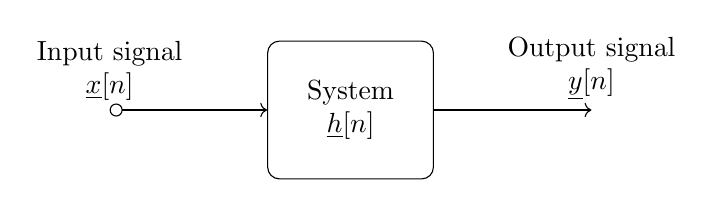
\begin{tikzpicture}
		\node[draw, block] (System) {System\\ $\underline{h}[n]$};
		\draw[<-o] (System.west) -- ++(-2cm, 0) node[above, align=center]{Input signal\\ $\underline{x}[n]$};
		\draw[->] (System.east) -- ++(2cm, 0) node[above, align=center]{Output signal\\ $\underline{y}[n]$};
	\end{tikzpicture}
	\caption{A time-discrete system with input and output}
\end{figure}

A time-discrete system is characterized by either
\begin{itemize}
	\item its \index{transfer function} transfer function
	\begin{equation}
		\underline{H}(\underline{z}) = \frac{\underline{Y}(\underline{z})}{\underline{X}(\underline{z})}
	\end{equation}
	or
	\item its impulse response.
	\begin{equation}
		\underline{h}[n] = \mathcal{Z}^{-1}\left\{\underline{H}(\underline{z})\right\}
	\end{equation}
\end{itemize}

In the time domain, the output is a convolution of the input and the impulse response.
\begin{equation}
	\underline{y}[n] = \underline{h}[n] * \underline{x}[n] = \sum\limits_{l = -\infty}^{\infty} \underline{h}[l] \underline{x}[n-l]
\end{equation}

The systems output is the impulse response $\underline{y}[n] = \underline{h}[n]$ if the input is a Kronecker delta function $\underline{x}[n] = \delta[n]$.
\begin{equation}
	\underline{h}[n] * \delta[n] = \underline{h}[n]
\end{equation}
Or in the frequency domain
\begin{equation}
	\underline{H}(\underline{z}) \cdot \underbrace{\mathcal{Z}\left\{\delta[n]\right\}}_{= 1} = \underline{H}(\underline{z})
\end{equation}

\begin{excursus}{Kronecker delta}
	The \index{Kronecker delta} Kronecker delta $\delta[n]$ equivalent of the Dirac delta function $\delta(t)$ in the discrete domain.
	
	\begin{equation*}
		\delta(t) = \begin{cases}
			\infty & \quad \text{if } t = 0, \\
			0 & \quad \text{if } t \neq 0.
		\end{cases}
	\end{equation*}
	
	\begin{equation*}
		\delta[n] = \begin{cases}
			1 & \quad \text{if } n = 0, \\
			0 & \quad \text{if } n \neq 0.
		\end{cases}
	\end{equation*}
	
	The Dirac delta function $\delta(t)$ is an indefinitely narrow pulse but indefinitely high. In contrast to that, the Kronecker delta $\delta[n]$ is of unity length and unity height. Both functions sum up to $1$.
	\begin{equation}
		\int\limits_{-\infty}^{\infty} \delta(t) \, \mathrm{d} t = \sum\limits_{n = -\infty}^{\infty} \delta[n] = 1
	\end{equation}
\end{excursus}

\subsection{Spectral Density}

\subsubsection{Cross-Correlation and Autocorrelation}

All considerations apply for ergodic or \ac{WSS} processes only:

\begin{itemize}
	\item Cross-correlation:
	\begin{equation}
		\underline{\mathrm{R}}_{xy}[n] = \left(\underline{x} \star \underline{y}\right)[n] = \sum\limits_{m=0}^{N-1} \underline{x}[m] \overline{\underline{y}[(m+n) \mod N]}
	\end{equation}
	\item Autocorrelation:
	\begin{equation}
		\underline{\mathrm{R}}_{xx}[n] = \left(\underline{x} \star \underline{x}\right)[n] = \sum\limits_{m=0}^{N-1} \underline{x}[m] \overline{\underline{x}[m+n]}
	\end{equation}
\end{itemize}

\subsubsection{Energy Spectral Density}

Parseval's theorem for discrete systems:
\begin{equation}
	\sum\limits_{n=0}^{N-1} \left|\underline{x}[n]\right|^2 = \frac{1}{N} \sum\limits_{k=0}^{N-1} \left|\underline{X}[k]\right|^2
\end{equation}

The signal energy is defined to:
\begin{equation}
	E = T_S^2 \sum\limits_{n=0}^{N-1} \left|\underline{x}[n]\right|^2 \stackrel{!}{=} \sum\limits_{n=0}^{N-1} \underline{\mathrm{S}}_{E,xx}[k]
\end{equation}
The sampling period $T_S$ (spacing between the samples) must be kept, because the physical energy depends on the duration of the samples.

The energy spectral density is:
\begin{equation}
	\underline{\mathrm{S}}_{E,xx}[k] = \frac{T_S^2}{N} \left|\underline{X}[k]\right|^2
\end{equation}

\subsubsection{Power Spectral Density}

The signal power is:
\begin{equation}
	P = \frac{T_S^2}{T} \sum\limits_{n=0}^{N-1} \left|\underline{x}[n]\right|^2 \stackrel{!}{=} \sum\limits_{n=0}^{N-1} \underline{\mathrm{S}}_{xx}[k]
\end{equation}
Where $T = N T_S$ is the duration of the signal.

Using the Parseval's theorem:
\begin{equation}
	\underline{\mathrm{S}}_{xx}[k] = \underline{\mathrm{S}}_{P,xx}[k] = \frac{T_S}{N} \sum\limits_{n=0}^{N-1} \left|\underline{X}[k]\right|^2
\end{equation}

\section{Digital Signals and Systems}

Now, we are in the time-discrete domain. However, values are still continuous.

Let's recapitulate the signal processing chain from the analogue to digital signals from Chapter 1:
\begin{figure}[H]
	\centering
	\begin{adjustbox}{scale=0.8}
		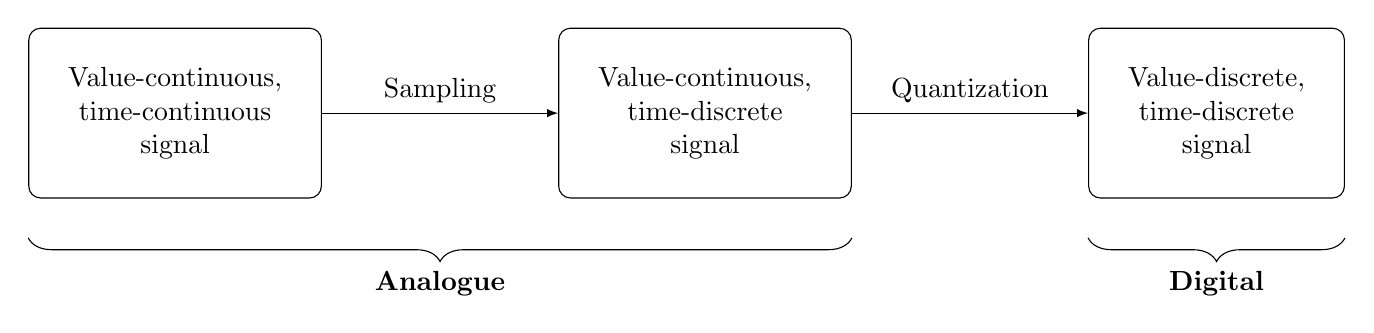
\begin{tikzpicture}
		\draw node[draw, block](Continuous){Value-continuous,\\ time-continuous\\ signal};
		\draw node[draw, block, right=3cm of Continuous](Sampled){Value-continuous,\\ time-discrete\\ signal};
		\draw node[draw, block, right=3cm of Sampled](Digital){Value-discrete,\\ time-discrete\\ signal};
		
		\draw [-latex] (Continuous) -- node[midway, align=center, above]{Sampling} (Sampled);
		\draw [-latex] (Sampled) -- node[midway, align=center, above]{Quantization} (Digital);
		
		\draw[decorate, decoration={brace, amplitude=3mm, mirror}] ([yshift=-5mm] Continuous.south west) -- ([yshift=-5mm] Sampled.south east) node[midway, below, yshift=-3mm]{\textbf{Analogue}};
		\draw[decorate, decoration={brace, amplitude=3mm, mirror}] ([yshift=-5mm] Digital.south west) -- ([yshift=-5mm] Digital.south east) node[midway, below, yshift=-3mm]{\textbf{Digital}};
		\end{tikzpicture}
	\end{adjustbox}
	\caption{Conversion from analogue to digital signals (recap from Chapter 1)}
	\label{fig:ch04:signals_sampling_recap}
\end{figure}

The device converting an analogue signal to a digital signal is a \index{analog-to-digital converter} \textbf{\ac{ADC}}. An \ac{ADC} comprises the two processes \emph{sampling} and \emph{quantization}.

\subsection{Quantization}

Quantization is the process of
\begin{itemize}
	\item \textbf{mapping} the continuous (analogue) values of the samples to a finite set of discrete (digital) of values
	\item by \textbf{rounding} and \textbf{truncating} the values.
\end{itemize}

\begin{figure}[H]
	\centering
	\begin{tikzpicture}
		\begin{axis}[
			height={0.25\textheight},
			width=0.6\linewidth,
			scale only axis,
			xlabel={$n$},
			ylabel={$x$},
			%grid style={line width=.6pt, color=lightgray},
			%grid=both,
			xmajorgrids=false,
			ymajorgrids=true,
			grid style={color=lightgray, dashed},
			legend pos=north east,
			axis y line=middle,
			axis x line=middle,
			every axis x label/.style={
				at={(ticklabel* cs:1.05)},
				anchor=north,
			},
			every axis y label/.style={
				at={(ticklabel* cs:1.05)},
				anchor=east,
			},
			xmin=0,
			xmax=7,
			ymin=0,
			ymax=3,
			xtick={0, 1, ..., 6},
			ytick={0, 0.5, ..., 2.5}
		]
			\addplot[smooth, blue, dashed] coordinates {(0, 1.1) (1, 1.8) (2, 2.1) (3, 1.0) (4, 0.8) (5, 1.7) (6, 2.4)};
			\addplot[red, thick] coordinates {(0, 0) (0, 1.0)};
			\addplot[red, thick] coordinates {(1, 0) (1, 2.0)};
			\addplot[red, thick] coordinates {(2, 0) (2, 2.0)};
			\addplot[red, thick] coordinates {(3, 0) (3, 1.0)};
			\addplot[red, thick] coordinates {(4, 0) (4, 1.0)};
			\addplot[red, thick] coordinates {(5, 0) (5, 1.5)};
			\addplot[red, thick] coordinates {(6, 0) (6, 2.5)};
			\addplot[only marks, red, thick, mark=o] coordinates {(0, 1.0) (1, 2.0) (2, 2.0) (3, 1.0) (4, 1.0) (5, 1.5) (6, 2.5)};
		\end{axis}
	\end{tikzpicture}
	\caption[A digital, value-discrete, time-discrete signal]{A digital, value-discrete, time-discrete signal. Only certain time points and a limited set of values (in this case multiples of $0.5$) are valid. (Recap from Chapter 1)}
	\label{fig:ch04:recap2}
\end{figure}

The mapping is an irreversible function $\mathcal{Q}\left\{\cdot\right\}$.

\begin{definition}{Quantization}
	In this chapter, the process of quantization is denoted by $\mathcal{Q}\left\{\cdot\right\}$. The digital signal $\underline{x}_Q[n]$ can be distinguished by its index $Q$ from its analogue counterpart $\underline{x}[n]$.
	\begin{equation}
		\underline{x}_Q[n] = \mathcal{Q}\left\{\underline{x}[n]\right\}
	\end{equation}%
	\nomenclature[Fq]{$\mathcal{Q}\left\{\cdot\right\}$}{Quantization}
	
	Later chapters will assume digital signals, unless noted otherwise. The index $Q$ will not be used there.
\end{definition}

The finite set of discrete numbers has the length $K$.
\begin{itemize}
	\item There are $K$ possible, unique values of $\underline{x}_Q[n]$.
	\item Usually, $K$ is a power of $2$. $K = 2^M$. $M$ is the number of bits.
\end{itemize}

\subsubsection{Linear Rounding Quantizer}

Rounding is a common model for quantization. \textit{Remark:} There are other methods like dead-zone quantizers, which are not subject to this lecture. Refer to literature about electronics to get a comprehensive overview.

The most common implementations distribute the $K$ discrete values equally between an interval of the continuous values $[\underline{\hat{X}}_L, \underline{\hat{X}}_H]$. So, the discrete values are spaced by
\begin{equation}
	\Delta \underline{\hat{X}} = \frac{\underline{\hat{X}}_H - \underline{\hat{X}}_L}{K - 1} \qquad \forall \, K \geq 2, K \in \mathbb{N}
\end{equation}
The mapping between $\underline{x}[n]$ and $\underline{x}_Q[n]$ is therefore \emph{linear}.

\begin{figure}[H]
	\centering
	\begin{tikzpicture}
		\begin{axis}[
			height={0.4\textheight},
			width=0.8\linewidth,
			scale only axis,
			xlabel={$x[n]$},
			ylabel={$x_Q[n]$},
			%grid style={line width=.6pt, color=lightgray},
			%grid=both,
			xmajorgrids=false,
			ymajorgrids=true,
			grid style={color=lightgray, dashed},
			legend pos=north east,
			axis y line=middle,
			axis x line=middle,
			every axis x label/.style={
				at={(ticklabel* cs:1.05)},
				anchor=north,
			},
			every axis y label/.style={
				at={(ticklabel* cs:1.05)},
				anchor=east,
			},
			xticklabel style={rotate=90, anchor=east},
			xmin=0,
			xmax=9,
			ymin=0,
			ymax=9,
			xtick={0, 1, ..., 8},
			xticklabels={$0$, $\hat{X}_L = \hat{X}_L + 0 \Delta \hat{X}$, $\hat{X}_L + 1 \Delta \hat{X}$, $\hat{X}_L + 2 \Delta \hat{X}$, $\hat{X}_L + 3 \Delta \hat{X}$, $\hat{X}_L + 4 \Delta \hat{X}$, $\hat{X}_L + 5 \Delta \hat{X}$, $\hat{X}_L + 6 \Delta \hat{X}$, $\hat{X}_H = \hat{X}_L + 7 \Delta \hat{X}$},
			ytick={0, 1, ..., 8},
			yticklabels={$0$, $\hat{X}_L = \hat{X}_L + 0 \Delta \hat{X}$, $\hat{X}_L + 1 \Delta \hat{X}$, $\hat{X}_L + 2 \Delta \hat{X}$, $\hat{X}_L + 3 \Delta \hat{X}$, $\hat{X}_L + 4 \Delta \hat{X}$, $\hat{X}_L + 5 \Delta \hat{X}$, $\hat{X}_L + 6 \Delta \hat{X}$, $\hat{X}_H = \hat{X}_L + 7 \Delta \hat{X}$},
		]
			\addplot[red, thick] coordinates {(0, 1) (1.5, 1)};
			\addplot[red, thick, dashed] coordinates {(1.5, 1) (1.5, 2)};
			\pgfplotsinvokeforeach{2, 3, ..., 7}{
				\addplot[red, thick] coordinates {({#1-0.5}, #1) ({#1+0.5}, #1)};
				\addplot[red, thick, dashed] coordinates {({#1+0.5}, #1) ({#1+0.5}, {#1+1})};
			}
			\addplot[red, thick] coordinates {(7.5, 8) (9, 8)};
		\end{axis}
	\end{tikzpicture}
	\caption[A rounding quantizer with linear mapping and a set of $K = 8$ discrete values]{A rounding quantizer with linear mapping and a set of $K = 8$ discrete values. All values $x[n] < \hat{X}_L$ are mapped to $\hat{X}_L$ and all values $x[n] > \hat{X}_H$ are mapped to $\hat{X}_H$.}
	\label{fig:ch04:linear_ammping}
\end{figure}


\begin{figure}[H]
	\centering
	\begin{circuitikz}
		\node[op amp] (Cmp1){};
		\node[op amp, below=1.5cm of Cmp1] (Cmp2){};
		\node[below=1cm of Cmp2] (Cmpx){$\vdots$};
		\node[op amp, below=1cm of Cmpx] (Cmpn){};
		
		\draw (Cmp1.-) to[short] ++(-1cm, 0);
		\draw (Cmp2.-) to[short] ++(-1cm, 0);
		\draw (Cmpn.-) to[short] ++(-1cm, 0);
		\draw ([shift={(-1cm,1.5cm)}] Cmp1.-) node[vcc]{$U_{ref}$} to[R,l=$\frac{1}{2}R$,-*] ([shift={(-1cm,0)}] Cmp1.-)
			to[R,l=$R$,-*] ([shift={(-1cm,0)}] Cmp2.-)
			to[short] ++(0,-1.5cm)
			to[open] ([shift={(-1cm,1.5cm)}] Cmpn.-)
			to[short,-*] ([shift={(-1cm,0)}] Cmpn.-)
			to[short] ([shift={(-1cm,-1.5cm)}] Cmpn.-)
			to[R,l=$\frac{1}{2}R$] ([shift={(-1cm,-3cm)}] Cmpn.-) node[rground]{};
			
		\draw ([shift={(-4cm,0)}] Cmp1.+) node[left]{$u_{in}(t)$} to[short,o-] (Cmp1.+);
		\draw ([shift={(-2cm,0)}] Cmp1.+) to[short,*-] ([shift={(-2cm,0)}] Cmp2.+) to[short,-] (Cmp2.+);
		\draw ([shift={(-2cm,0)}] Cmp2.+) to[short,*-] ++(0,-1cm);
		\draw ([shift={(-2cm,2cm)}] Cmpn.+) to[short,-] ([shift={(-2cm,0)}] Cmpn.+) to[short,-] (Cmpn.+);
		
		\node[below] at([shift={(-1cm,-1.5cm)}] Cmp2.-){$\vdots$};
		\node[below] at([shift={(-2cm,-1cm)}] Cmp2.+){$\vdots$};
		
		\draw (Cmpn.out) to[short,-o] ++(2cm,0) node[right,align=left]{$1 \quad \text{if } u_{in}(t) \geq \frac{1}{K-1} U_{ref}$};
		\draw (Cmp2.out) to[short,-o] ++(2cm,0) node[right,align=left]{$1 \quad \text{if } u_{in}(t) \geq \frac{K-3}{K-1} U_{ref}$};
		\draw (Cmp1.out) to[short,-o] ++(2cm,0) node[right,align=left]{$1 \quad \text{if } u_{in}(t) \geq \frac{K-2}{K-1} U_{ref}$};
	\end{circuitikz}
	\caption[An example quantizer circuit implementing the rounding quantization using comparators]{An example quantizer circuit implementing the rounding quantization using comparators. $K$ resistors $R$ and $K-1$ linearly quantize $u_{in}$ into $K$ discrete values. The range is \SI{0}{V} to $U_{ref}$.}
\end{figure}

\textit{Remark:} There are other mappings like logarithmic mapping. However, this lecture only considers linear mapping.

\subsection{Pulse-Code Modulation}

One piece of the \ac{ADC} is missing. So far, we a have quantized, discrete signal $\underline{x}_Q[n]$.

\begin{itemize}
	\item To be processed by a computer, the values of $\underline{x}_Q[n]$ must be coded in way a computer can handle.
	\item A computer processes signals with two discrete states $0$ and $1$. These binary signals are called \index{bit} \textbf{bits}.
	\item Multiple bits are grouped to symbols.
	\begin{itemize}
		\item \index{nibble} 1 nibble: 4 bits
		\item \index{byte} 1 byte: 8 bits
		\item \index{word} 1 word: natural data size of a computer architecture (most commonly 32 bits or 64 bits)
	\end{itemize}
\end{itemize}

The discrete values of $\underline{x}_Q[n]$ are coded as computer readable symbols. This mapping is called \index{pulse-code modulation} \textbf{\ac{PCM}}.

\begin{table}[H]
	\centering
	\caption[Example PCM for $K = 8$]{Example \ac{PCM} for $K = 8$}
	\begin{tabular}{|l|r|r|}
		\hline
		$\underline{x}_Q[n]$ & Data & Data (binary) \\
		\hline
		\hline
		$\hat{X}_L = \hat{X}_L + 0 \Delta \hat{X}$ & 0 & 000 \\
		\hline
		$\hat{X}_L + 1 \Delta \hat{X}$ & 1 & 001 \\
		\hline
		$\hat{X}_L + 2 \Delta \hat{X}$ & 2 & 010 \\
		\hline
		$\hat{X}_L + 3 \Delta \hat{X}$ & 3 & 011 \\
		\hline
		$\hat{X}_L + 4 \Delta \hat{X}$ & 4 & 100 \\
		\hline
		$\hat{X}_L + 5 \Delta \hat{X}$ & 5 & 101 \\
		\hline
		$\hat{X}_L + 6 \Delta \hat{X}$ & 6 & 110 \\
		\hline
		$\hat{X}_H = \hat{X}_L + 7 \Delta \hat{X}$ & 7 & 111 \\
		\hline
	\end{tabular}
\end{table}

The complete processing chain of the \ac{PCM}, implemented by an \ac{ADC}, be completed to:
\begin{figure}[H]
	\centering
	\begin{adjustbox}{scale=0.8}
		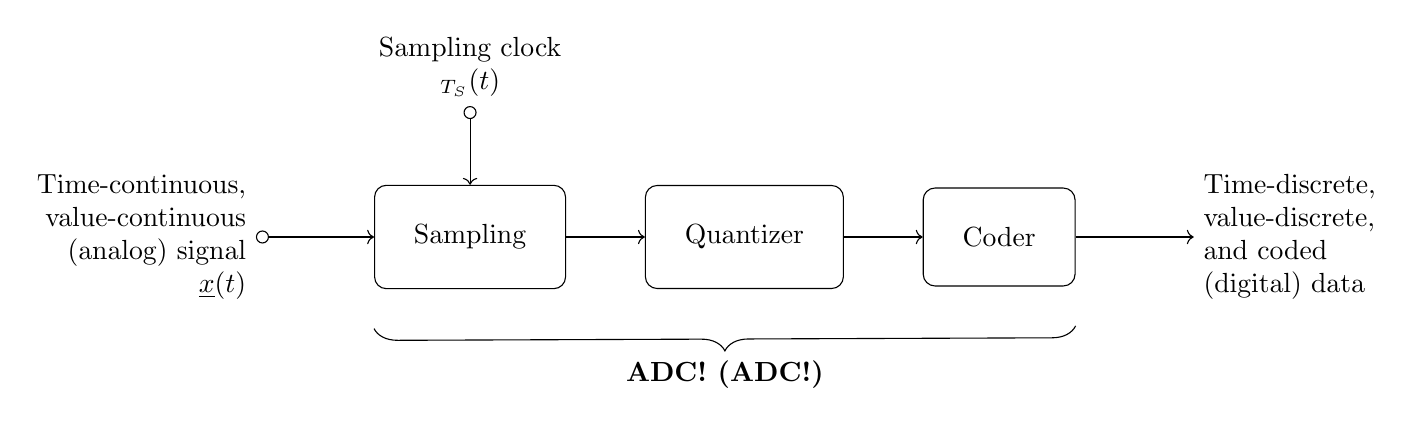
\begin{tikzpicture}
			\node[draw, block] (Sampler){Sampling};
			\node[draw, block, right=1cm of Sampler] (Quantizer){Quantizer};
			\node[draw, block, right=1cm of Quantizer] (Coder){Coder};
			
			\draw[o->] ([xshift=-1.5cm] Sampler.west) node[left,align=right]{Time-continuous,\\ value-continuous\\ (analog) signal\\ $\underline{x}(t)$} -- (Sampler.west);
			\draw[->] (Sampler.east) -- (Quantizer.west);
			\draw[->] (Quantizer.east) -- (Coder.west);
			\draw[->] (Coder.east) -- ++(1.5cm,0) node[right,align=left]{Time-discrete,\\ value-discrete,\\ and coded\\ (digital) data};
			
			\draw[o->] ([yshift=1cm] Sampler.north) node[above, align=center]{Sampling clock\\ $\Sha_{T_S}(t)$} -- (Sampler.north);
			
			\draw[decorate, decoration={brace, amplitude=3mm, mirror}] ([yshift=-5mm] Sampler.south west) -- ([yshift=-5mm] Coder.south east) node[midway, below, yshift=-3mm]{\textbf{\acf{ADC}}};
		\end{tikzpicture}
	\end{adjustbox}
	\caption[Generating a PCM signal from an analogue signal $\underline{x}(t)$ using an ADC]{Generating a \ac{PCM} signal from an analogue signal $\underline{x}(t)$ using an \ac{ADC}}
	\label{fig:ch04:signals_to_data}
\end{figure}

\subsection{Quantization Noise}

Once values have been quantized, their original, continuous values cannot be reconstructed.

\begin{fact}
	The process of quantization is irreversible.
\end{fact}

Furthermore, the quantized values differ from their original value due to rounding and truncation. This difference $\underline{e}[n]$ is the \index{quantization error} \textbf{quantization error}.

\begin{definition}{Quantization error}
	Each value-discrete (quantized) value $\underline{x}_Q[n]$ has an error $\underline{e}[n]$ from its original, value-continuous, analogue value $\underline{x}[n]$.
	\begin{equation}
		\underline{x}_Q[n] = \mathcal{Q}\left\{\underline{x}[n]\right\} = \underline{x}[n] + \underline{e}[n]
	\end{equation}
	
	The error is bounded to
	\begin{equation}
		\left|\underline{e}[n]\right| \leq \frac{1}{2} \left|\Delta \underline{\hat{X}}\right|
	\end{equation}
\end{definition}

\subsubsection{Quantization Error of PCM Data}

\ac{PCM} data is usually coded as symbols consisting of $B$ (binary) bits.
\begin{itemize}
	\item Subsequent symbols have a spacing of $1$ (unity spacing).
	\item The \ac{PCM} normalizes the value spacing of the quantizer $\underline{\hat{X}}$ to unity spacing $1$.
	\item A corollary is that the quantization error $\left|\underline{\tilde{e}}[n]\right| = \frac{1}{2}$.
\end{itemize}
For example if the \ac{PCM} value is $\left(10010100\right)_2$, its real value is between $\left(10010011\right)_2$ (equivalent to $\left(10010100\right)_2 - 0.5$) and $\left(10010110\right)_2$ (equivalent to $\left(10010100\right)_2 + 0.5$).

\begin{itemize}
	\item The quantization error of a \ac{PCM} signal resides in \ac{LSB}.
	\item The quantization error is uniformly distributed between $\SI{-1/2}{LSB} = -2^{-B}$ and $\SI{+1/2}{LSB} = +2^{-B}$, where $B$ is the number of bits.
\end{itemize}

\begin{excursus}{The \ac{LSB}}
	A binary number can be decomposed:
	\begin{equation}
		\left(10010101\right)_2 = 1 \cdot 2^7 + 0 \cdot 2^6 + 0 \cdot 2^5 + 1 \cdot 2^4 + 1 \cdot 2^3 + 1 \cdot 2^2 + 0 \cdot 2^1 + 1 \cdot 2^0
	\end{equation}%
	\nomenclature[Nb]{$\left(\cdot\right)_2$}{Binary number}%
	\nomenclature[Nh]{$\left(\cdot\right)_{16}$}{Hexadecimal number}%
	\nomenclature[Nd]{$\left(\cdot\right)_{10}$}{Explicit decimal number}
	
	The \index{least significant bit} \textbf{\ac{LSB}} is the digit with the exponent $2^0$.
\end{excursus}

%TODO
%\todo{Plot error}

The quantization error superimposes the original signal and is therefore noise -- the \index{quantization noise} \textbf{quantization noise}.

The \emph{quantization noise power} of the error, which is distributed between $-2^{-B}$ and $+2^{-B}$, is:
\begin{equation}
	P_{Q,N} = \hat{X}_H^2 2^{B-1} \int\limits_{-2^{-B}}^{+2^{-B}} e^2 \, \mathrm{d} e = \frac{\hat{X}_H^2}{3 \cdot 4^B}
\end{equation}
where $\hat{X}_H$ is the highest discrete value of the quantizer for input signals $x[n]$.

\begin{definition}{The \acf{SQNR}}
	A \ac{SNR} which is referenced to the quantization noise is called \index{signal-to-qunatization-noise ratio} \textbf{\acf{SQNR}}.
	\begin{equation}
		\mathrm{SQNR} = \frac{P_{Q,S}}{P_{Q,N}} = \frac{P_{Q,S} \cdot 3 \cdot 4^B}{\hat{X}_H^2}
	\end{equation}
	where $\hat{X}_H$ is the highest discrete value of the quantizer for input signals $x[n]$.
	Or in the logarithmic scale:
	\begin{equation}
		\begin{split}
			L_{\mathrm{SQNR}} &= \SI{10}{dB} \log_{10}\left(\frac{P_{Q,S}}{P_{Q,N}}\right) \\
			 &= \SI{10}{dB} \log_{10}\left(\frac{P_{Q,S} \cdot 3 \cdot 4^B}{\hat{X}_H^2}\right) \\
			 &= \SI{10}{dB} \log_{10}\left(\frac{P_{Q,S}}{\hat{X}_H^2}\right) + \SI{4.77}{dB} + B \cdot \SI{6.02}{dB}
		\end{split}
	\end{equation}
\end{definition}

%TODO Is this correct?
%As a rule of thumb,
%\begin{itemize}
%	\item The overall \ac{SNR} is the \ac{SQNR} for \underline{strong} input signals. The quantization noise dominates the thermal noise.
%	\item The overall \ac{SNR} is the signal-to-thermal-noise ratio for \underline{weak} input signals. The quantization noise is dominated by the thermal noise.
%\end{itemize}

\subsubsection{Dynamic Range}

The maximum range of a quantizer is $\hat{X}_H - \hat{X}_L$. $\hat{X}_L$ is zero is most applications. $\hat{X}_H$ is the highest discrete value of the quantizer for input signals $x[n]$.

An important characteristic of an \ac{ADC} is its \emph{resolution}. It is approximately $\frac{\hat{X}_H}{2^B}$.

Let's consider the \ac{SQNR} for a sine wave at maximum amplitude $\hat{X}_H$. The power of the quantized sine wave is:
\begin{equation}
	P_{Q,S} = \frac{1}{2} \hat{X}_H^2
\end{equation}
The \ac{SQNR} is:
\begin{equation}
	\left.L_{\mathrm{SQNR}}\right|_{\text{Sine}} = \SI{10}{dB} \log_{10}\left(\frac{1}{2}\right) + \SI{4.77}{dB} + B \cdot \SI{6.02}{dB} = \SI{1.761}{dB} + B \cdot \SI{6.02}{dB}
\end{equation}

The \ac{SQNR} of a sine wave is the \index{dynamic range} \textbf{dynamic range} of an \ac{ADC}.
\begin{definition}{Dynamic range of an \ac{ADC}}
	\begin{equation}
		L_{\mathrm{DR}} = \SI{1.761}{dB} + B \cdot \SI{6.02}{dB}
	\end{equation}
\end{definition}

The dynamic range increases, when more bits $B$ are added. However, the number of bits $B$ correlates with the complexity of the \ac{ADC} hardware. Therefore, a trade-off between sufficient dynamic range and reasonable hardware complexity must be chosen. Typical bit numbers:
\begin{itemize}
	\item $B = 8$ to $B = 10$ for \ac{RF} applications with high sampling rates ($> \SI{1}{MHz}$),
	\item $B = 16$ or $B = 24$ for audio applications with medium sampling rates ($\approx \SI{44}{kHz}$).
\end{itemize}

%\begin{excursus}{\si{dBFS}}
%	When talking about signals in relation to an \ac{ADC}, they are referenced.
%\end{excursus}

%\subsubsection{Quantization Noise Floor}
%
%Analogous to the thermal noise floor,

\subsection{Synchronization 1: Time Recovery}

For wideband \ac{RF} applications, the sampling rate is chosen close to the maximum frequency of the signal, so that the Shannon-Nyquist sampling theorem can be fulfilled.

The sampling rate $f_S$ is not the only important parameter. The time instance at which the sample is taken must fit, too. Thus, both period and phase of the Dirac comb $\Sha_{T_S}(t)$ used by the sampler must fit.

The problem with a non-optimal sampling phase is depicted below. The difference between the current sample timing and the optimal sample timing is the \index{timing error} \textbf{timing error}.

\begin{figure}[H]
	\centering
	\subfloat[Optimal sample timing]{
		\centering
		\begin{tikzpicture}
			\begin{axis}[
				height={0.20\textheight},
				width=0.6\linewidth,
				scale only axis,
				xlabel={$t$},
				ylabel={$x$},
				%grid style={line width=.6pt, color=lightgray},
				%grid=both,
				grid=none,
				legend pos=outer north east,
				axis y line=middle,
				axis x line=middle,
				every axis x label/.style={
					at={(ticklabel* cs:1.05)},
					anchor=north,
				},
				every axis y label/.style={
					at={(ticklabel* cs:1.05)},
					anchor=east,
				},
				xmin=0,
				xmax=4.5,
				ymin=-1.2,
				ymax=1.2,
				xtick={0, 1, ..., 4},
				ytick={-1, -0.5, ..., 1}
			]
				\addplot[red, smooth, domain=0:4, samples=50] plot (\x, {cos(deg(pi*\x))});
				\addlegendentry{Original signal};
				\addplot[green, dashed, smooth, domain=0:4, samples=50] plot (\x, {cos(deg(pi*\x))});
				\addlegendentry{Sampled signal};
				\addplot[blue, only marks, mark=o] coordinates {(0, 1) (1, -1) (2, 1) (3, -1) (4, 1)};
				\addlegendentry{Sample times};
			\end{axis}
		\end{tikzpicture}
	}

	\subfloat[Non-optimal sample timing]{
		\centering
		\begin{tikzpicture}
			\begin{axis}[
				height={0.20\textheight},
				width=0.6\linewidth,
				scale only axis,
				xlabel={$t$},
				ylabel={$x$},
				%grid style={line width=.6pt, color=lightgray},
				%grid=both,
				grid=none,
				legend pos=outer north east,
				axis y line=middle,
				axis x line=middle,
				every axis x label/.style={
					at={(ticklabel* cs:1.05)},
					anchor=north,
				},
				every axis y label/.style={
					at={(ticklabel* cs:1.05)},
					anchor=east,
				},
				xmin=0,
				xmax=4.5,
				ymin=-1.7,
				ymax=1.2,
				xtick={0, 1, ..., 4},
				ytick={-1, -0.5, ..., 1}
			]
				\addplot[red, smooth, domain=0:4, samples=50] plot (\x, {cos(deg(pi*\x))});
				\addlegendentry{Original signal};
				\addplot[green, dashed, smooth, domain=0:4, samples=50] plot (\x, {0.707*cos(deg(pi*\x-(pi/4)))});
				\addlegendentry{Sampled signal};
				\addplot[blue, only marks, mark=o] coordinates {(0.25, 0.707) (1.25, -0.707) (2.25, 0.707) (3.25, -0.707)};
				\addlegendentry{Sample times};
				
				\draw[dashed] (axis cs:2,1.2) -- (axis cs:2,-1.2);
				\draw[dashed] (axis cs:2.25,1.2) -- (axis cs:2.25,-1.2);
				\draw[<->] (axis cs:2,-1.1) -- node[midway,yshift=-2mm,below,align=center]{Timing error} (axis cs:2.25,-1.1);
			\end{axis}
		\end{tikzpicture}
	}
	
	\subfloat[Poor sample timing]{
		\centering
		\begin{tikzpicture}
			\begin{axis}[
				height={0.20\textheight},
				width=0.6\linewidth,
				scale only axis,
				xlabel={$t$},
				ylabel={$x$},
				%grid style={line width=.6pt, color=lightgray},
				%grid=both,
				grid=none,
				legend pos=outer north east,
				axis y line=middle,
				axis x line=middle,
				every axis x label/.style={
					at={(ticklabel* cs:1.05)},
					anchor=north,
				},
				every axis y label/.style={
					at={(ticklabel* cs:1.05)},
					anchor=east,
				},
				xmin=0,
				xmax=4.5,
				ymin=-1.7,
				ymax=1.2,
				xtick={0, 1, ..., 4},
				ytick={-1, -0.5, ..., 1}
			]
				\addplot[red, smooth, domain=0:4, samples=50] plot (\x, {cos(deg(pi*\x))});
				\addlegendentry{Original signal};
				\addplot[green, dashed] coordinates {(0, 0) (4, 0)};
				\addlegendentry{Sampled signal};
				\addplot[blue, only marks, mark=o] coordinates {(0.5, 0) (1.5, 0) (2.5, 0) (3.5, 0)};
				\addlegendentry{Sample times};
				
				\draw[dashed] (axis cs:2,1.2) -- (axis cs:2,-1.2);
				\draw[dashed] (axis cs:2.5,1.2) -- (axis cs:2.5,-1.2);
				\draw[<->] (axis cs:2,-1.1) -- node[midway,yshift=-2mm,below,align=center]{Timing error} (axis cs:2.5,-1.1);
			\end{axis}
		\end{tikzpicture}
	}
	\caption[Different situations of sample timing]{Different situations of sample timing. In this example, the signal frequency is close to half of the sampling rate (maximum allowed frequency according to the Nyquist-Shannon sampling theorem).}
	\label{fig:ch04:timing_error}
\end{figure}

The phase (time offset) of the sampler must be adjusted to obtain an optimal sample timing. This adjustment is called \index{timing recovery} \textbf{timing recovery}. The goal is to reduce the \emph{timing error} to zero.

There are different approaches to implement the timing recovery:
\begin{itemize}
	\item Analogue timing recovery (with forward prediction)
	\item Hybrid timing recovery (with closed control loop)
	\item Digital timing recovery (with forward prediction or closed control loop)
\end{itemize}

\begin{figure}[H]
	\centering
	\begin{adjustbox}{scale=0.8}
		\begin{circuitikz}
			\node[draw, block] at(0,0) (Sampler){Sampler};
			\node[oscillator, below=of Sampler](Clock){};
			\node[draw, block, left=of Clock] (Filter){Loop filter};
			\node[draw, block, left=of Filter] (Pred){Timing error\\ prediction};
			
			\draw[dashed] (Sampler.north) -- ++(0, 2cm) node[below left, align=right]{Analogue\\ domain} node[below right, align=left]{Digital\\ domain};
			\node[right=2mm of Clock, align=left]{Sampling clock};
			
			\draw[o->] (-11,0) node[left,align=right]{Input} -- (Sampler.west);
			\draw[->] (Sampler.east) -- ++(1.5,0) node[right,align=left]{Further signal\\ processing};
			
			\draw[*->] (-10,0) |- (Pred.west);
			\draw[->] (Pred.east) -- (Filter.west);
			\draw[->] (Filter.east) -- (Clock.west);
			\draw[->] (Clock.north) -- (Sampler.south);
		\end{circuitikz}
	\end{adjustbox}
	\caption{Analogue timing recovery (with forward prediction)}
\end{figure}

\begin{figure}[H]
	\centering
	\begin{adjustbox}{scale=0.8}
		\begin{circuitikz}
			\node[draw, block] at(0,0) (Sampler){Sampler};
			\node[oscillator, below=of Sampler](Clock){};
			\node[draw, block, right=of Clock] (Filter){Loop filter};
			\node[draw, block, right=of Filter] (Pred){Timing error\\ estimator};
			
			\draw[dashed] (Sampler.north) -- ++(0, 2cm) node[below left, align=right]{Analogue\\ domain} node[below right, align=left]{Digital\\ domain};
			\node[left=2mm of Clock, align=right]{Sampling clock};
			
			\draw[o->] (-2.5,0) node[left,align=right]{Input} -- (Sampler.west);
			\draw[->] (Sampler.east) -- ++(11,0) node[right,align=left]{Further signal\\ processing};
			
			\draw[*->] (10,0) |- (Pred.east);
			\draw[->] (Pred.west) -- (Filter.east);
			\draw[->] (Filter.west) -- (Clock.east);
			\draw[->] (Clock.north) -- (Sampler.south);
		\end{circuitikz}
	\end{adjustbox}
	\caption{Hybrid timing recovery (with closed control loop)}
\end{figure}

\begin{figure}[H]
	\centering
	\begin{adjustbox}{scale=0.8}
		\begin{circuitikz}
			\node[draw, block] at(0,0) (Sampler){Sampler};
			\node[oscillator, below=of Sampler](Clock){};
			\node[draw, block, right=of Sampler] (Resampler){Interpolation\\ and resampling};
			\node[draw, block, below=of Resampler] (Filter){Loop filter};
			\node[draw, block, right=of Filter] (Pred){Timing error\\ estimator};
			
			\draw[dashed] (Sampler.north) -- ++(0, 2cm) node[below left, align=right]{Analogue\\ domain} node[below right, align=left]{Digital\\ domain};
			\node[left=2mm of Clock, align=right]{Free-running\\ sampling clock};
			
			\draw[o->] (-2.5,0) node[left,align=right]{Input} -- (Sampler.west);
			\draw[->] (Sampler.east) -- (Resampler.west);
			\draw[->] (Resampler.east) -- ++(6,0) node[right,align=left]{Further signal\\ processing};
			
			\draw[*->] (11,0) |- (Pred.east);
			\draw[->] (Pred.west) -- (Filter.east);
			\draw[->] (Filter.north) -- (Resampler.south);
			
			\draw[->] (Clock.north) -- (Sampler.south);
		\end{circuitikz}
	\end{adjustbox}
	\caption{Digital timing recovery (with closed control loop)}
\end{figure}

There various algorithms to implement the timing recovery, which will not be discussed in detail in this lecture.

%\subsection{Practical Issues}

\phantomsection
\addcontentsline{toc}{section}{References}
\printbibliography[heading=subbibliography]
\end{refsection}


\clearpage
% SPDX-License-Identifier: CC-BY-SA-4.0
%
% Copyright (c) 2020 Philipp Le
%
% Except where otherwise noted, this work is licensed under a
% Creative Commons Attribution-ShareAlike 4.0 License.
%
% Please find the full copy of the licence at:
% https://creativecommons.org/licenses/by-sa/4.0/legalcode

\phantomsection
\addcontentsline{toc}{section}{Exercise 4}
\section*{Exercise 4}

%%%%%%%%%%%%%%%%%%%%%%%%%%%%%%%%%%%%%%%%%%%%%%%%%%%%%%%%%%%%%%%%%%%%%%%%%%%%%%%
\begin{question}[subtitle={Sampling Periodic Signals}]
	\begin{equation*}
		u(t) = \SI{2}{V} \cdot \cos\left(2\pi \cdot \SI{2}{MHz} \cdot t + \SI{60}{\degree}\right)
	\end{equation*}
	The signal is sampled with a sampling period of $T_S = \SI{125}{\nano\second}$. The first sample taken is $u(t = 0)$.
	
	\begin{tasks}
		\task
		Plot the function from $t = 0$ to $t = \SI{1}{\micro\second}$!
		
		\task
		Calculate the samples $n = 0 \dots 8$!
		
		\task
		What is the DTFT of the signal?
		
		Hints:
		\begin{equation*}
			\begin{split}
				x[n] = e^{-j a n} &= \underline{X}_{2\pi}\left(e^{-j \phi}\right) = 2 \pi \sum\limits_{l = -\infty}^{\infty} \delta \left(\phi + a - 2\pi l\right) \\
				\cos\left(b\right) &= \frac{1}{2} \left(e^{j b} + e^{-j b}\right)
			\end{split}
		\end{equation*}
		
		\task
		Can the DFT directly applied to the signal? If yes, determine the smallest $N$ and give the values of all $\underline{U}[k]$!
		
		\task
		What is the longest possible sampling period? What must be considered at this sampling period?
		
		\task
		Now, the sampling period is changed to $T_S = \SI{0.5}{\micro\second}$. There is no anti-aliasing filter. The reconstruction filter is an ideal low-pass filter with a cut-off frequency of $\SI{2.5}{MHz}$. Give the reconstructed output function in the time domain! Give an explanation in the frequency domain!
	\end{tasks}
\end{question}

\begin{solution}
	\begin{tasks}
		\task
		\begin{figure}[H]
			\centering
			\begin{tikzpicture}
				\begin{axis}[
					height={0.25\textheight},
					width=0.8\linewidth,
					scale only axis,
					xlabel={$t$ in \si{\micro\second}},
					ylabel={$u(t)$},
					%grid style={line width=.6pt, color=lightgray},
					%grid=both,
					grid=none,
					legend pos=outer north east,
					axis y line=middle,
					axis x line=middle,
					every axis x label/.style={
						at={(ticklabel* cs:1.05)},
						anchor=north,
					},
					every axis y label/.style={
						at={(ticklabel* cs:1.05)},
						anchor=east,
					},
					xmin=-0.1,
					xmax=1.1,
					ymin=-2.2,
					ymax=2.2,
					xtick={0,0.125,...,1},
					%xticklabels={$- \omega_S$, $- \frac{\omega_S}{2}$, $0$, $\frac{\omega_S}{2}$, $\omega_S$},
					%ytick={0},
				]
					\addplot[blue, dashed, smooth, domain=0:1, samples=50] plot(\x, {2*cos(deg(2*pi*2*\x)+60)});
					%\addlegendentry{$u(t)$};
					\pgfplotsinvokeforeach{0,0.125,...,1}{
						\addplot[red] coordinates {(#1,0) (#1,{2*cos(deg(2*pi*2*#1)+60)})};
						\addplot[red, only marks, mark=o] coordinates {(#1,{2*cos(deg(2*pi*2*#1)+60)})};
					}
				\end{axis}
			\end{tikzpicture}
		\end{figure}
	
		\task
		\begin{table}[H]
			\centering
			\begin{tabular}{|l|r|r|r|r|r|r|r|r|r|}
				\hline
				$n$ & $0$ & $1$ & $2$ & $3$ & $4$ & $5$ & $6$ & $7$ & $8$
\\
				\hline
				$t$ in \si{\micro\second} & $0.0$ & $0.125$ & $0.25$ & $0.375$ & $0.5$ & $0.625$ & $0.75$ & $0.875$ & $1.0$
\\
				\hline
				\hline
				$u[n]$ in \si{V} & $1.0$ & $-1.73$ & $-1.0$ & $1.73$ & $1.0$ & $-1.73$ & $-1.0$ & $1.73$ & $1.0$ \\
				\hline
			\end{tabular}
		\end{table}
		
		\task
		$t = n T_S$ due to the sampling:
		\begin{equation*}
			\begin{split}
				u[n] &= \SI{2}{V} \cdot \cos\left(2\pi \cdot \SI{2}{MHz} \cdot n T_S + \SI{60}{\degree}\right) \\
				 &= \SI{1}{V} \cdot \left( e^{j \left(2\pi \cdot \SI{2}{MHz} \cdot n T_S + \SI{60}{\degree}\right)} + e^{-j \left(2\pi \cdot \SI{2}{MHz} \cdot n T_S + \SI{60}{\degree}\right)} \right) \\
				 &= \SI{1}{V} \cdot \left( e^{j \SI{60}{\degree}} \cdot e^{j \cdot 2\pi \cdot \SI{2}{MHz} \cdot n T_S} + e^{-j \SI{60}{\degree}} \cdot e^{-j \cdot 2\pi \cdot \SI{2}{MHz} \cdot n T_S} \right)
			\end{split}
		\end{equation*}
		
		The DTFT is:
		\begin{equation*}
			\begin{split}
				\underline{U}_{2\pi}\left(e^{-j \phi}\right) &= \SI{2}{V} \cdot \pi \sum\limits_{l = -\infty}^{\infty} \left( e^{j \SI{60}{\degree}} \cdot \delta\left(\phi - \left(2\pi \cdot \SI{2}{MHz} \cdot T_S\right) - 2\pi l\right)\right. \\ &\qquad + \left.e^{-j \SI{60}{\degree}} \cdot \delta\left(\phi + \left(2\pi \cdot \SI{2}{MHz} \cdot T_S\right) - 2\pi l\right) \right)
			\end{split}
		\end{equation*}
		
		\task
		Yes, it is periodic with $T_0=\SI{500}{ns}$. This means:
		\begin{equation*}
			N = \frac{T_0}{T_S} = 4
		\end{equation*}
		
		The DFT over $N=4$ is:
		\begin{equation*}
			\begin{split}
				\underline{X}[k] &= \sum\limits_{n=0}^{N-1} \underline{x}[n] \cdot e^{-j 2\pi \frac{k}{N} n}
			\end{split}
		\end{equation*}
		\begin{equation*}
			\begin{split}
				\phi[k] &= 2 \pi \frac{k}{N} \\
				\omega[k] &= \frac{\phi[k]}{T_S} \\
				f[k] &= \frac{\omega[k]}{2 \pi} \\
			\end{split}
		\end{equation*}
		
		\begin{table}[H]
			\centering
			\begin{tabular}{|l|r|r|r|r|}
				\hline
				$k$ & $0$ & $1$ & $2$ & $3$
\\
				\hline
				$k$ (alternate) & $0$ & $1$ & $-2$ & $-1$ \\
				\hline
				\hline
				$\phi[k]$ & $0$ & $1.57 \approx \pi$ & $3.14 \approx 2 \pi \equiv -2\pi$ & $4.71 \approx 3 \pi \equiv -\pi$ \\
				\hline
				$\omega[k]$ & $\SI{0}{{\micro\second}^{-1}}$ & $\SI{12.57}{{\micro\second}^{-1}}$ & $\SI{25.13}{{\micro\second}^{-1}}$ & $\SI{37.7}{{\micro\second}^{-1}}$ \\
				\hline
				$f[k]$ & $\SI{0}{MHz}$ & $\SI{2}{MHz}$ & $\SI{4}{MHz} \equiv \SI{-4}{MHz}$ & $\SI{6}{MHz} \equiv \SI{-2}{MHz}$ \\
				\hline
				\hline
				$\underline{U}[k]$ & $0$ & $(2+3.46j)$ & $0$ & $(2-3.46j)$ \\
				\hline
				$|\underline{U}[k]|$ & $0.0$ & $4.0$ & $0.0$ & $4.0$ \\
				\hline
				$\arg\left(\underline{U}[k]\right)$ & $\SI{3.14}{rad} \approx \SI{360}{\degree}$ & $\SI{1.05}{rad} \approx \SI{60}{\degree}$ & $\SI{3.14}{rad} \approx \SI{360}{\degree}$ & $\SI{-1.05}{rad} \approx \SI{-60}{\degree}$ \\
				\hline
			\end{tabular}
		\end{table}
	
		\task
		\begin{itemize}
			\item Minimum possible sampling frequency is \SI{4}{MHz}. Anything below, will violate the Shannon-Nyquist theorem and cause aliasing.
			\item The longest possible sampling period is therefore \SI{250}{ns}.
			\item At $T_S = \SI{250}{ns}$, the sampling phase must be considered, too.
			\begin{itemize}
				\item It must be shifted by $\SI{+60}{\degree}$, so that the maxima of $u(t)$ are sampled.
				\item This retains the amplitude of \SI{2}{V}.
				\item A timing error will effectively reduce the amplitude of the sampled signal in relation to the original signal.
				\item At a timing error of $\Delta T_S = \SI{125}{ns}$, all samples will be zero, because the Dirac comb used for sampling is orthogonal to the original signal.
			\end{itemize}
		\end{itemize}
	
		\task
		The sampling period of \SI{500}{ns} violates the Shannon-Nyquist theorem and causes aliasing.
		
		\begin{figure}[H]
			\subfloat[Original signal $\underline{U}\left(j\omega\right)$] {
				\centering
				\begin{tikzpicture}
					\begin{axis}[
						height={0.15\textheight},
						width=0.25\linewidth,
						scale only axis,
						xlabel={$\omega$},
						ylabel={$|\underline{U}\left(j\omega\right)|$},
						%grid style={line width=.6pt, color=lightgray},
						%grid=both,
						grid=none,
						legend pos=north east,
						axis y line=middle,
						axis x line=middle,
						every axis x label/.style={
							at={(ticklabel* cs:1.05)},
							anchor=north,
						},
						every axis y label/.style={
							at={(ticklabel* cs:1.05)},
							anchor=east,
						},
						xmin=-1.5,
						xmax=1.5,
						ymin=0,
						ymax=1.2,
						xtick={-1, -0.5, 0, 0.5, 1},
						xticklabels={$- \omega_S$, $- \frac{\omega_S}{2}$, $0$, $\frac{\omega_S}{2}$, $\omega_S$},
						ytick={0},
						%ytick={0, 1},
						%yticklabels={0, $\SI{}$}
					]
						\draw[-latex, red, very thick] (axis cs:1,0) -- (axis cs:1,0.8); %node[left,align=right,anchor=north,rotate=90,yshift=-5mm]{$\arg\left(\underline{U}\left(j\omega_S\right)\right) = \SI{60}{\degree}$};
						\draw[-latex, green, very thick] (axis cs:-1,0) -- (axis cs:-1,0.8); %node[left,align=right,anchor=north,rotate=90,yshift=-5mm]{$\arg\left(\underline{U}\left(-j\omega_S\right)\right) = \SI{-60}{\degree}$};
					\end{axis}
				\end{tikzpicture}
			}
			\hfill
			\subfloat[Spectrum of the Dirac comb $\frac{2 \pi}{T} \Sha_{\frac{2 \pi}{T}}(\omega)$] {
				\centering
				\begin{tikzpicture}
					\begin{axis}[
						height={0.15\textheight},
						width=0.27\linewidth,
						scale only axis,
						xlabel={$t$},
						ylabel={$|\frac{2 \pi}{T} \Sha_{\frac{2 \pi}{T}}(\omega)|$},
						%grid style={line width=.6pt, color=lightgray},
						%grid=both,
						grid=none,
						legend pos=north east,
						axis y line=middle,
						axis x line=middle,
						every axis x label/.style={
							at={(ticklabel* cs:1.05)},
							anchor=north,
						},
						every axis y label/.style={
							at={(ticklabel* cs:1.05)},
							anchor=east,
						},
						xmin=-2.5,
						xmax=2.5,
						ymin=0,
						ymax=1.2,
						xtick={-2, ..., 2},
						xticklabels={$-2 \omega_S$, $- \omega_S$, $0$, $\omega_S$, $2 \omega_S$},
						ytick={0},
					]
						\pgfplotsinvokeforeach{-3, -2, ..., 3}{
							\draw[-latex, blue, very thick] (axis cs:#1,0) -- (axis cs:#1,1);
						}
					\end{axis}
				\end{tikzpicture}
			}
			\hfill
			\subfloat[Sampled signal $\underline{U}_S\left(j\omega\right)$, showing aliasing] {
				\centering
				\begin{tikzpicture}
					\begin{axis}[
						height={0.15\textheight},
						width=0.27\linewidth,
						scale only axis,
						xlabel={$\omega$},
						ylabel={$|\underline{U}_S\left(j\omega\right)|$},
						%grid style={line width=.6pt, color=lightgray},
						%grid=both,
						grid=none,
						legend pos=north east,
						axis y line=middle,
						axis x line=middle,
						every axis x label/.style={
							at={(ticklabel* cs:1.05)},
							anchor=north,
						},
						every axis y label/.style={
							at={(ticklabel* cs:1.05)},
							anchor=east,
						},
						xmin=-2.5,
						xmax=2.5,
						ymin=0,
						ymax=1.2,
						xtick={-2, -1, -0.5, 0, 0.5, 1, 2},
						xticklabels={$-2 \omega_S$, $- \omega_S$, $- \frac{\omega_S}{2}$, $0$, $\frac{\omega_S}{2}$, $\omega_S$, $2 \omega_S$},
						ytick={0},
					]
						\pgfplotsinvokeforeach{-3, -2, ..., 3}{
							\draw[-latex, blue, dashed, very thick] (axis cs:#1,0) -- (axis cs:#1,1);
							\draw[-latex, green, very thick] (axis cs:{#1-0.01},0) -- (axis cs:{#1-0.01},0.8);
							\draw[-latex, red, very thick] (axis cs:{#1+0.01},0) -- (axis cs:{#1+0.01},0.8);
						}
					\end{axis}
				\end{tikzpicture}
			}
		\end{figure}
	
		\begin{itemize}
			\item The spectral components of $\SI{+2}{MHz}$ (with $e^{j \SI{60}{\degree}}$) and $\SI{-2}{MHz}$ (with $e^{j \SI{-60}{\degree}}$) superimpose at \SI{0}{Hz} (DC).
			\item The resulting component at \SI{0}{Hz} is the addition if two complex numbers (see Part c) ):
			\begin{equation*}
				\underline{U}_S\left(j 0\right) = \SI{2}{V} \cdot \pi \underbrace{\left(e^{j \SI{60}{\degree}} + e^{j \SI{-60}{\degree}}\right)}_{= 1}  \delta(\omega) = \SI{2}{V} \cdot \pi \cdot  \delta(\omega)
			\end{equation*}
			\item Applying the reconstruction filter gives the spectrum of the reconstructed signal:
			\begin{equation*}
				\underline{U}_R\left(j \omega\right) = \SI{2}{V} \cdot \pi \cdot \delta(\omega)
			\end{equation*}
			\item The inverse DTFT is:
			\begin{equation*}
				u_R(t) = \SI{1.0}{V}
			\end{equation*}
			\item The reconstructed signal is a DC signal of \SI{1.0}{V}.
		\end{itemize}
	
		\begin{figure}[H]
			\centering
			\begin{tikzpicture}
				\begin{axis}[
					height={0.15\textheight},
					width=0.8\linewidth,
					scale only axis,
					xlabel={$t$ in \si{\micro\second}},
					ylabel={$u(t)$},
					%grid style={line width=.6pt, color=lightgray},
					%grid=both,
					grid=none,
					legend pos=outer north east,
					axis y line=middle,
					axis x line=middle,
					every axis x label/.style={
						at={(ticklabel* cs:1.05)},
						anchor=north,
					},
					every axis y label/.style={
						at={(ticklabel* cs:1.05)},
						anchor=east,
					},
					xmin=-0.1,
					xmax=1.1,
					ymin=-2.2,
					ymax=2.2,
					xtick={0,0.125,...,1},
					%xticklabels={$- \omega_S$, $- \frac{\omega_S}{2}$, $0$, $\frac{\omega_S}{2}$, $\omega_S$},
					%ytick={0},
				]
					\addplot[blue, dashed, smooth, domain=0:1, samples=50] plot(\x, {2*cos(deg(2*pi*2*\x)+60)});
					\addlegendentry{$u(t)$};
					\addplot[olive] coordinates {(0,1) (0.5,1) (1,1)};
					\addlegendentry{$u_R(t)$};
					\pgfplotsinvokeforeach{0,0.5,1}{
						\addplot[red] coordinates {(#1,0) (#1,{2*cos(deg(2*pi*2*#1)+60)})};
						\addplot[red, only marks, mark=o] coordinates {(#1,{2*cos(deg(2*pi*2*#1)+60)})};
					}
				\end{axis}
			\end{tikzpicture}
		\end{figure}
	\end{tasks}
\end{solution}

%%%%%%%%%%%%%%%%%%%%%%%%%%%%%%%%%%%%%%%%%%%%%%%%%%%%%%%%%%%%%%%%%%%%%%%%%%%%%%%
\begin{question}[subtitle={Sampling Non-Periodic Signals}]
	The signal $x[n]$ is given in the time domain.
	\begin{table}[H]
		\centering
		\begin{tabular}{|l|r|r|r|r|r|r|r|r|}
			\hline
			$n$ & 0 & 1 & 2 & 3 & 4 & 5 & 6 & 7 \\
			\hline
			\hline
			$x[n]$ & 0.25 & 1 & -0.5 & 0.5 & -0.5 & -1 & -0.5 & -0.75 \\
			\hline
		\end{tabular}
	\end{table}
	
	\begin{tasks}
		\task
		The signal is windowed with $N = 4$ starting at $x[n = 0]$. A hamming window with $M = 2$ is applied. Calculate the values of $\underline{x}_W[n]$!
		
		Hamming window:
		\begin{equation*}
			w[n] = \begin{cases}0.54 - 0.46 \cos\left(\frac{2 \pi n}{M}\right), &\quad 0 \leq n \leq M,\\ 0, &\quad \text{otherwise}.\end{cases}
		\end{equation*}
		
		\task
		Calculate the discrete Fourier transform of the windowed signal!
		
		\task
		The signal has been sampled with $T_S = \SI{1}{ms}$. What frequency values do the $k$ represent?
	\end{tasks}
\end{question}

\begin{solution}
	\begin{tasks}
		\task
		At first the signal is truncated. Only the first $4$ samples are considered.
		
		The window function is:
		\begin{equation*}
			w[n] = \begin{cases}0.54 - 0.46 \cos\left(\frac{2 \pi n}{M}\right), &\quad 0 \leq n \leq M,\\ 0, &\quad \text{otherwise}.\end{cases}
		\end{equation*}
		
		The signal is then multiplied with the window:
		\begin{equation*}
			x_w[n] = x[n] \cdot w[n]
		\end{equation*}
		
		\begin{table}[H]
			\centering
			\begin{tabular}{|l|r|r|r|r|}
				\hline
				$n$ & 0 & 1 & 2 & 3 \\
				\hline
				\hline
				$w[n]$ & 0.08 & 1.0 & 0.08 & 0 \\
				\hline
				$x_w[n]$ & 0.02 & 1.0 & -0.04 & 0 \\
				\hline
			\end{tabular}
		\end{table}
		
		\task
		The signal is periodically repeated.
		
		The DFT is calculated over $N = 4$.
		\begin{equation*}
			\underline{X}_w[k] = \mathcal{F}_{\text{DFT}}\left\{\underline{x}[n]\right\} = \sum\limits_{n \in N} \underline{x}[n] \cdot e^{-j 2\pi \frac{k}{N} n}
		\end{equation*}
		
		\begin{table}[H]
			\centering
			\begin{tabular}{|l|r|r|r|r|}
				\hline
				$k$ & 0 & 1 & 2 & 3 \\
				\hline
				$k$ (alternate) & 0 & 1 & -2 & -1 \\
				\hline
				\hline
				$\underline{X}_w[k]$ & $0.98$ & $(0.06-1j)$ & $-1.02$ & $(0.06+1j)$ \\
				\hline
				$|\underline{X}_w[k]|$ & $0.98$ & $1.00$ & $1.02$ & $1.00$ \\
				\hline
				$\arg\left(\underline{X}_w[k]\right)$ & $0$ & $-1.51 \approx -\pi$ & $3.14 \approx 2\pi$ & $1.51 \approx \pi$ \\
				\hline
			\end{tabular}
		\end{table}
	
		\task
		\begin{equation*}
			\begin{split}
				\phi[k] &= 2 \pi \frac{k}{N} \\
				\omega[k] &= \frac{\phi[k]}{T_S} \\
				f[k] &= \frac{\omega[k]}{2 \pi} \\
			\end{split}
		\end{equation*}
		
		\begin{table}[H]
			\centering
			\begin{tabular}{|l|r|r|r|r|}
				\hline
				$k$ & 0 & 1 & 2 & 3 \\
				\hline
				$k$ (alternate) & 0 & 1 & -2 & -1 \\
				\hline
				\hline
				$\phi[k]$ & $0$ & $1.57 \approx \pi$ & $3.14 \approx 2 \pi \equiv -2\pi$ & $4.71 \approx 3 \pi \equiv -\pi$ \\
				\hline
				$\omega[k]$ & $\SI{0}{s^{-1}}$ & $\SI{1570.8}{s^{-1}}$ & $\SI{3141.6}{s^{-1}}$ & $\SI{4712.4}{s^{-1}}$ \\
				\hline
				\hline
				$f[k]$ & $\SI{0}{Hz}$ & $\SI{250}{Hz}$ & $\SI{500}{Hz} \equiv \SI{-500}{Hz}$ & $\SI{750}{Hz} \equiv \SI{-250}{Hz}$ \\
				\hline
			\end{tabular}
		\end{table}
	\end{tasks}
\end{solution}

%%%%%%%%%%%%%%%%%%%%%%%%%%%%%%%%%%%%%%%%%%%%%%%%%%%%%%%%%%%%%%%%%%%%%%%%%%%%%%%
\begin{question}[subtitle={Quantization}]
	The signal of Task 1b) is now quantized. The quantizer has $8$ discrete values. These values are equally distributed between \SI{-2}{V} and \SI{2}{V}. Prior to sampling, the original time-continuous signal passed through an ideal low-pass filter with a cut-off frequency of \SI{4}{MHz}.
	
	\begin{tasks}
		\task
		Define a mapping from the value-continuous samples to the value-discrete samples!
		
		\task
		The value-discrete samples are now pulse-code modulated. How many bits are required?
		
		\task
		What is the resulting data (signal from Task 1b) )?
		
		\task
		Determine the quantization error for each value-discrete sample! How much is the signal-to-quantization-noise ratio?
		
		\task
		3 bits are a very poor resolution. How many bits are appropriate for the quantizer to obtain the best signal-to-noise ratio? Effects of the window filter are neglected. Assume that the signal has passed through a processing chain with a total gain of \SI{24}{dB}, noise figure of \SI{12}{dB} and bandwidth of \SI{4}{MHz} prior to quantization. The input of the quantizer has an impedance of \SI{50}{\ohm}. % 14 bits
	\end{tasks}
\end{question}

\begin{solution}
	\begin{tasks}
		\task
		\begin{itemize}
			\item $\hat{U}_L = \SI{-2}{V}$
			\item $\hat{U}_H = \SI{2}{V}$
			\item $K = 8$
		\end{itemize}
		\begin{equation*}
			\Delta \hat{U} = \frac{\hat{U}_H - \hat{U}_L}{K - 1} = \SI{0.57}{V}
		\end{equation*}
		
		The boundaries for the rounding quantizer are distributed $\pm \frac{1}{2} \Delta \hat{U}$ around each mean.
		\begin{table}[H]
			\begin{tabular}{|r|r|r|r|}
				\hline
				From & To & Maps to & PCM data \\
				\hline
				\hline
				$-\infty$ & $\SI{-1.71}{V}$ & $\SI{-2.0}{V}$ & 0
\\
				$\SI{-1.71}{V}$ & $\SI{-1.14}{V}$ & $\SI{-1.43}{V}$ & 1
\\
				$\SI{-1.14}{V}$ & $\SI{-0.57}{V}$ & $\SI{-0.86}{V}$ & 2
\\
				$\SI{-0.57}{V}$ & $\SI{-0.0}{V}$ & $\SI{-0.29}{V}$ & 3
\\
				$\SI{0.0}{V}$ & $\SI{0.57}{V}$ & $\SI{0.29}{V}$ & 4
\\
				$\SI{0.57}{V}$ & $\SI{1.14}{V}$ & $\SI{0.86}{V}$ & 5
\\
				$\SI{1.14}{V}$ & $\SI{1.71}{V}$ & $\SI{1.43}{V}$ & 6
\\
				$\SI{1.71}{V}$ & $\infty$ & $\SI{2.0}{V}$ & 7 \\
				\hline
			\end{tabular}
		\end{table}
	
		\task
		\begin{equation*}
			B \geq \log_2 \left(K\right) = 3
		\end{equation*}
		Minimum 3 bits.
		
		\task
		\begin{table}[H]
			\centering
			\begin{tabular}{|l|r|r|r|r|r|}
				\hline
				$n$ & $0$ & $1$ & $2$ & $3$ & $4$
\\
				\hline
				\hline
				$u[n]$ in \si{V} & $1.0$ & $-1.73$ & $-1.0$ & $1.73$ & $1.0$ \\
				\hline
				Quantized values in \si{V} & $0.86$ & $-2.0$ & $-0.86$ & $2.0$ & $0.86$ \\
				\hline
				PCM data & $\left(101\right)_2$ & $\left(000\right)_2$ & $\left(010\right)_2$ & $\left(111\right)_2$ & $\left(101\right)_2$ \\
				\hline
				\hline
				$n$ & $5$ & $6$ & $7$ & $8$ &
\\
				\hline
				\hline
				$u[n]$ in \si{V} & $-1.73$ & $-1.0$ & $1.73$ & $1.0$ & \\
				\hline
				Quantized values in \si{V} & $-2.0$ & $-0.86$ & $2.0$ & $0.86$ & \\
				\hline
				PCM data & $\left(000\right)_2$ & $\left(010\right)_2$ & $\left(111\right)_2$ & $\left(101\right)_2$ & \\
				\hline
			\end{tabular}
		\end{table}
	
		\task
		\begin{table}[H]
			\centering
			\begin{tabular}{|l|r|r|r|r|r|}
				\hline
				$n$ & $0$ & $1$ & $2$ & $3$ & $4$
\\
				\hline
				\hline
				$u[n]$ in \si{V} & $1.0$ & $-1.73$ & $-1.0$ & $1.73$ & $1.0$ \\
				\hline
				Quantized values in \si{V} & $0.86$ & $-2.0$ & $-0.86$ & $2.0$ & $0.86$ \\
				\hline
				Quantization error in \si{V} & $0.14$ & $0.27$ & $0.14$ & $0.27$ & $0.14$ \\
				\hline
				\hline
				$n$ & $5$ & $6$ & $7$ & $8$ &
\\
				\hline
				\hline
				$u[n]$ in \si{V} & $-1.73$ & $-1.0$ & $1.73$ & $1.0$ & \\
				\hline
				Quantized values in \si{V} & $-2.0$ & $-0.86$ & $2.0$ & $0.86$ & \\
				\hline
				Quantization error in \si{V} & $0.27$ & $0.14$ & $0.27$ & $0.14$ & \\
				\hline
			\end{tabular}
		\end{table}
	
		The signal-to-quantization-noise ratio for the sine wave is:
		\begin{equation*}
			\mathrm{SQNR} = \SI{1.761}{dB} + B \cdot \SI{6.02}{dB} = \SI{19.82}{dB}
		\end{equation*}
		
		\task
		\begin{itemize}
			\item The RMS value of the signal is $U_{\mathrm{RMS}} = \frac{\SI{2}{V}}{\sqrt{2}} = \SI{1.41}{V}$
			\item The signal power is $P_S = \frac{U_{\mathrm{RMS}}^2}{R} = \SI{39.8}{mW} \equiv L_{P,S} = \SI{16}{dBm}$
			\item The thermal noise floor is $\SI{-174}{dBm/Hz}$
			\item At $\SI{4}{MHz} \equiv \SI{66}{dBHz}$, the thermal noise power is $\SI{-174}{dBm/Hz} + \SI{66}{dBHz} = \SI{-108}{dBm}$
			\item The gain and noise factor is applied to the thermal noise, resulting in a noise power of $L_{P,N} = \SI{-108}{dBm} + \SI{24}{dB} + \SI{12}{dB} = \SI{-70}{dBm}$
			\item \textit{Note that the gain is not applied to the signal power, because it is already known/given at the quantizer input.}
			\item The signal-to-noise ratio is $L_{\mathrm{SNR}} = L_{P,S} - L_{P,N} = \SI{16}{dBm} - \SI{-71}{dBm} = \SI{86}{dB}$
			\item The signal-to-quantization-noise ratio should not be grater than the signal-to-noise ratio, because otherwise the thermal noise would dominate the quantization noise.
			\begin{equation*}
				L_{\mathrm{SQNR}} \stackrel{!}{=} L_{\mathrm{SNR}}
			\end{equation*}
			\item The number of bits must be at least
			\begin{equation*}
				B \geq \frac{L_{\mathrm{SQNR}} - \SI{1.761}{dB}}{\SI{6.02}{dB}} = 14
			\end{equation*}
		\end{itemize}
	\end{tasks}
\end{solution}

%%%%%%%%%%%%%%%%%%%%%%%%%%%%%%%%%%%%%%%%%%%%%%%%%%%%%%%%%%%%%%%%%%%%%%%%%%%%%%%
%\begin{question}[subtitle={Decibel}]
%	\begin{tasks}
%	\end{tasks}
%\end{question}
%
%\begin{solution}
%	\begin{tasks}
%	\end{tasks}
%\end{solution}

\clearpage

% SPDX-License-Identifier: CC-BY-SA-4.0
%
% Copyright (c) 2020 Philipp Le
%
% Except where otherwise noted, this work is licensed under a
% Creative Commons Attribution-ShareAlike 4.0 License.
%
% Please find the full copy of the licence at:
% https://creativecommons.org/licenses/by-sa/4.0/legalcode

\chapter{Modulation and Mixing}

\begin{refsection}
	
The task of a communication system is transmitting information.

Example: Voice transmission
\begin{itemize}
	\item Voice has a spectrum from about \SI{20}{Hz} to \SI{20}{kHz}
	\item It is not feasible to transmit the spectrum directly as electromagnetic waves.
	\item The electromagnetic spectrum must be shared with myriads of other users.
	\item So, the voice is shifted to a higher frequency, for example, \SI{144.3}{MHz}.
	\item The voice is \emph{modulated} on this \emph{carrier} of \SI{144.3}{MHz}.
	\item The voice is then located from about \SI{144.28}{MHz} to \SI{144.32}{MHz}.
\end{itemize}

\begin{definition}{Modulation}
	\index{modulation} \textbf{Modulation} is the process of altering a signal -- the \index{carrier} \textbf{carrier} -- so that it contains the information to be transmitted.
\end{definition}

\begin{definition}{Demodulation}
	\index{demodulation} \textbf{Demodulation} is the inverse process of modulation. The information is extracted from the carrier.
\end{definition}

In the previous example, the voice was the information-carrying signal. This can be transferred to any kind of information. In this chapter, we will discuss techniques to modulate data on carriers which can be transmitted over wired and wireless channels.

\todo{Block diagram modulator}

\section{Modulation in The Time and Frequency Domain}

Generally, the carrier is a \emph{monochromatic} signal, i.e., it is a sinusoidal function. A sinusoidal function has three parameters: (angular) frequency $\omega_C$, phase $\varphi_C$ and amplitude $\hat{X}_C$.
\begin{equation}
	x_C(t) = \hat{X}_C \cos\left(\omega_C t + \varphi_C\right)
	\label{eq:ch05:carrier_timedomain}
\end{equation}
The frequency is fixed to the carrier frequency. The other two parameters can be altered and the information can be modulated into them.

There are two classes of modulation:
\begin{itemize}
	\item \textbf{Amplitude modulation} The amplitude of the carrier is altered.
	\begin{equation}
		x_{S,AM}(t) = f_{\hat{X}}(t) \cos\left(\omega_C t + \varphi_C\right)
	\end{equation}
	\item \textbf{Phase modulation} The phase of the carrier is altered.
	\begin{equation}
		x_{S,PM}(t) = \hat{X}_C \cos\left(\omega_C t + f_{\varphi}(t)\right)
	\end{equation}
\end{itemize}

This section covers basic modulation techniques of analogue signals.
\begin{itemize}
	\item The considerations are explanatory and are extended to digital signals in the following section.
	\item This section shall offer an understanding of how modulation works in general (for both analogue and digital signals).
	\item A digital signal must be converted to an analogue signal in order to physically exists. It can then be modulated onto a carrier and transmitted as an electromagnetic wave.
\end{itemize}

\subsection{Amplitude Modulation}

The \index{amplitude modulation} \textbf{\ac{AM}} is the alteration of the carrier's amplitude.

\begin{attention}
	By now, all signals are real, because the technical realization is considered. Physical signals must always be real.
\end{attention}

The carrier is a mono-chromatic signal:
\begin{equation}
	x_C(t) = \hat{X}_C \cdot \cos\left(2\pi f_C + \varphi_C\right)
\end{equation}
where
\begin{itemize}
	\item $\hat{X}_C$ is the amplitude of the carrier,
	\item $f_C$ is the carrier frequency ($2\pi f_C = \omega_C$ is carrier angular frequency), and
	\item $\varphi_C$ is the phase offset of the carrier.
\end{itemize}

The carrier amplitude can be altered by multiplying it with the instantaneous value of the information-carrying signal $x_B(t)$:
\begin{equation}
	x_{DSB-TC}(t) = x_B(t) \cdot \left(1 + \mu x_C(t)\right)
	\label{eq:ch05:amdsb_timedomain}
\end{equation}
\begin{itemize}
	\item The waveform of the carrier is retained. The carrier is still present in the modulated signal. This is represented by the $+1$ in the sum.
	\item Its amplitude is changed by the instantaneous value of the information-carrying signal. The contribution of the information-carrying signal is defined by the factor $\mu$.
\end{itemize}

\begin{figure}[H]
	\centering
	
	\subfloat[Carrier and information-carrying signals]{
		\centering
		\begin{tikzpicture}
			\begin{axis}[
				height={0.15\textheight},
				width=0.6\linewidth,
				scale only axis,
				xlabel={$t$},
				ylabel={$x(t)$},
				%grid style={line width=.6pt, color=lightgray},
				%grid=both,
				grid=none,
				legend pos=outer north east,
				axis y line=middle,
				axis x line=middle,
				every axis x label/.style={
					at={(ticklabel* cs:1.05)},
					anchor=north,
				},
				every axis y label/.style={
					at={(ticklabel* cs:1.05)},
					anchor=east,
				},
				xmin=-0.5,
				xmax=8.5,
				ymin=-1.2,
				ymax=1.2,
				%xtick={0,0.125,...,1},
				%xticklabels={$- \omega_S$, $- \frac{\omega_S}{2}$, $0$, $\frac{\omega_S}{2}$, $\omega_S$},
				%ytick={0},
			]
				\addplot[blue, smooth, domain=0:8, samples=200] plot(\x, {cos(deg(2*pi*2*\x))});
				\addlegendentry{Carrier $x_C(t)$};
				\addplot[red, smooth, domain=0:8, samples=50] plot(\x, {cos(deg(2*pi*0.25*\x))});
				\addlegendentry{Information $x_B(t)$};
			\end{axis}
		\end{tikzpicture}
	}

	\subfloat[\acs{DSB-TC} \acs{AM} (with carrier)]{
		\centering
		\begin{tikzpicture}
			\begin{axis}[
				height={0.15\textheight},
				width=0.6\linewidth,
				scale only axis,
				xlabel={$t$},
				ylabel={$x_{DSB-TC}(t)$},
				%grid style={line width=.6pt, color=lightgray},
				%grid=both,
				grid=none,
				legend pos=outer north east,
				axis y line=middle,
				axis x line=middle,
				every axis x label/.style={
					at={(ticklabel* cs:1.05)},
					anchor=north,
				},
				every axis y label/.style={
					at={(ticklabel* cs:1.05)},
					anchor=east,
				},
				xmin=-0.5,
				xmax=8.5,
				ymin=-1.7,
				ymax=1.7,
				%xtick={0,0.125,...,1},
				%xticklabels={$- \omega_S$, $- \frac{\omega_S}{2}$, $0$, $\frac{\omega_S}{2}$, $\omega_S$},
				%ytick={0},
			]
				\addplot[red, smooth, domain=0:8, samples=150] plot(\x, {cos(deg(2*pi*2*\x)) * (1+0.5*cos(deg(2*pi*0.25*\x)))});
				\addlegendentry{\acs{DSB} Signal $x_{DSB-TC}(t)$};
				\addplot[olive, dashed, smooth, domain=0:8, samples=150] plot(\x, {(1+0.5*cos(deg(2*pi*0.25*\x)))});
				\addlegendentry{Envelope of $x_B(t)$};
			\end{axis}
		\end{tikzpicture}
	}

	\caption{\acs{DSB} \acs{AM} of analogue signals}
\end{figure}

\subsubsection{Frequency Domain}

Assumptions for the information-carrying signal:
\begin{itemize}
	\item The information-carrying signal is band-limited to $-f_B \geq f \geq f_B$ ($\underline{X}_B\left(j\omega\right) = 0 \quad \forall \; |f| > f_B$).
	\item The information-carrying signal is real-valued. Its spectrum is therefore symmetric ($\underline{X}_B\left(j\omega\right) = \overline{\underline{X}_B\left(-j\omega\right)}$).
\end{itemize}

The carrier is monochromatic \eqref{eq:ch05:carrier_timedomain}. Its \ac{CTFT} is:
\begin{equation}
	\underline{X}_C\left(j\omega\right) = \hat{X}_C \pi \left( \delta\left(\omega + 2 \pi f_C \right) + \delta\left(\omega - 2 \pi f_C \right) \right)
\end{equation}

The time-domain expression \eqref{eq:ch05:amdsb_timedomain} of the \ac{AM} is in the frequency domain:
\begin{equation}
	\underline{X}_{DSB-TC}\left(j\omega\right) = \underline{X}_C\left(j\omega\right) + \mu \underline{X}_C\left(j\omega\right) * \underline{X}_B\left(j\omega\right)
\end{equation}
The multiplication becomes a convolution.
\begin{equation}
	\underline{X}_{DSB-TC}\left(j\omega\right) = \hat{X}_C \pi \left( \underbrace{\delta\left(\omega + 2 \pi f_C \right) + \mu \underline{X}_B\left(j\left(\omega + 2 \pi f_C\right)\right)}_{\text{Carrier plus frequency-shifted information (-)}} + \underbrace{\delta\left(\omega - 2 \pi f_C \right) + \mu \underline{X}_B\left(j\left(\omega - 2 \pi f_C\right)\right)}_{\text{Carrier plus frequency-shifted information (+)}} \right)
\end{equation}

\textbf{The \ac{AM} is a frequency shift of the information-carrying in both the positive and the negative direction.}

Due to the symmetry of the information-carrying signal, there is an \emph{upper sideband} and a \emph{lower sideband}, carrying the identical information, around the carrier.

Because of the presence of the carrier and both sidebands, the modulation is called \index{double-sideband!transmitted carrier} \textbf{\acf{DSB-TC}}.

\begin{definition}{Transmission bandwidth of \acs{DSB} \acs{AM}}
	The modulated signal of the \acs{DSB} \acs{AM} consists of the positive and negative part of the information-carrying signal shifted in frequency to the carrier frequency. The information-carrying signal emerges as sidebands.
	
	Therefore, the bandwidth of the modulated signal is $[\omega_C - \omega_B, \omega_C + \omega_B]$. The difference $2 \omega_B$ is called \index{transmission bandwidth} \textbf{transmission bandwidth}.
\end{definition}

\begin{fact}
	The transmission bandwidth of \acs{DSB} \acs{AM} is the double of the maximum frequency in the information-carrying signal $2 \omega_B$.
\end{fact}

\begin{figure}[H]
	\subfloat[Information-carrying signal $\underline{X}_B\left(j\omega\right)$ (real-valued in time-domain)] {
		\centering
		\begin{tikzpicture}
			\begin{axis}[
				height={0.15\textheight},
				width=0.9\linewidth,
				scale only axis,
				xlabel={$\omega$},
				ylabel={$|\underline{X}_B\left(j\omega\right)|$},
				%grid style={line width=.6pt, color=lightgray},
				%grid=both,
				grid=none,
				legend pos=north east,
				axis y line=middle,
				axis x line=middle,
				every axis x label/.style={
					at={(ticklabel* cs:1.05)},
					anchor=north,
				},
				every axis y label/.style={
					at={(ticklabel* cs:1.05)},
					anchor=east,
				},
				xmin=-3.5,
				xmax=3.5,
				ymin=0,
				ymax=1.2,
				xtick={-0.5, 0, 0.5},
				xticklabels={$- \omega_B$, $0$, $\omega_B$},
				ytick={0},
			]
				\draw[red, thick] (axis cs:-0.5,0) -- (axis cs:0,0.7);
				\draw[red, thick] (axis cs:0,0.7) -- (axis cs:0.5,0);
			\end{axis}
		\end{tikzpicture}
	}
	
	\subfloat[Carrier signal $\underline{X}_C\left(j\omega\right)$ (real-valued in time-domain)] {
		\centering
		\begin{tikzpicture}
			\begin{axis}[
				height={0.15\textheight},
				width=0.9\linewidth,
				scale only axis,
				xlabel={$\omega$},
				ylabel={$|\underline{X}_C\left(j\omega\right)|$},
				%grid style={line width=.6pt, color=lightgray},
				%grid=both,
				grid=none,
				legend pos=north east,
				axis y line=middle,
				axis x line=middle,
				every axis x label/.style={
					at={(ticklabel* cs:1.05)},
					anchor=north,
				},
				every axis y label/.style={
					at={(ticklabel* cs:1.05)},
					anchor=east,
				},
				xmin=-3.5,
				xmax=3.5,
				ymin=0,
				ymax=1.2,
				xtick={-2, 0, 2},
				xticklabels={$- \omega_C$, $0$, $\omega_C$},
				ytick={0},
			]
				\pgfplotsinvokeforeach{-2, 2}{
					\draw[-latex, blue, very thick] (axis cs:#1,0) -- (axis cs:#1,1);
				}
			\end{axis}
		\end{tikzpicture}
	}
	
	\subfloat[\acs{AM} \acs{DSB-TC} modulated signal $\underline{X}_{DSB-TC}\left(j\omega\right)$ with frequency-shifted information and carrier (real-valued in time-domain)] {
		\centering
		\begin{tikzpicture}
			\begin{axis}[
				height={0.15\textheight},
				width=0.9\linewidth,
				scale only axis,
				xlabel={$\omega$},
				ylabel={$|\underline{X}_{DSB-TC}\left(j\omega\right)|$},
				%grid style={line width=.6pt, color=lightgray},
				%grid=both,
				grid=none,
				legend pos=north east,
				axis y line=middle,
				axis x line=middle,
				every axis x label/.style={
					at={(ticklabel* cs:1.05)},
					anchor=north,
				},
				every axis y label/.style={
					at={(ticklabel* cs:1.05)},
					anchor=east,
				},
				xmin=-3.5,
				xmax=3.5,
				ymin=0,
				ymax=1.2,
				xtick={-2, 0, 2},
				xticklabels={$- \omega_C$, $0$, $\omega_C$},
				ytick={0},
			]
				\pgfplotsinvokeforeach{-2, 2}{
					\draw[-latex, red, very thick] (axis cs:#1,0) -- (axis cs:#1,1);
					\draw[red, thick] (axis cs:{#1-0.5},0) -- (axis cs:#1,0.7);
					\draw[red, thick] (axis cs:#1,0.7) -- (axis cs:{#1+0.5},0);
				}
			\end{axis}
		\end{tikzpicture}
	}
	
	\caption{Spectrum of the \acs{DSB-TC} \acs{AM} signal}
\end{figure}

\subsection{Carrier Suppression}

The carrier does not contain any information. It can therefore be removed from the modulated signal. The $+1$ of \eqref{eq:ch05:amdsb_timedomain} is dropped. The \ac{AM} becomes a simple multiplication.
\begin{equation}
	x_{DSB-SC}(t) = x_B(t) \cdot x_C(t)
	\label{eq:ch05:amdsbsc_timedomain}
\end{equation}

\begin{figure}[H]
	\centering
	
	\subfloat[Carrier and information-carrying signals]{
		\centering
		\begin{tikzpicture}
			\begin{axis}[
				height={0.15\textheight},
				width=0.6\linewidth,
				scale only axis,
				xlabel={$t$},
				ylabel={$x(t)$},
				%grid style={line width=.6pt, color=lightgray},
				%grid=both,
				grid=none,
				legend pos=outer north east,
				axis y line=middle,
				axis x line=middle,
				every axis x label/.style={
					at={(ticklabel* cs:1.05)},
					anchor=north,
				},
				every axis y label/.style={
					at={(ticklabel* cs:1.05)},
					anchor=east,
				},
				xmin=-0.5,
				xmax=8.5,
				ymin=-1.2,
				ymax=1.2,
				%xtick={0,0.125,...,1},
				%xticklabels={$- \omega_S$, $- \frac{\omega_S}{2}$, $0$, $\frac{\omega_S}{2}$, $\omega_S$},
				%ytick={0},
			]
				\addplot[blue, smooth, domain=0:8, samples=200] plot(\x, {cos(deg(2*pi*2*\x))});
				\addlegendentry{Carrier $x_C(t)$};
				\addplot[red, smooth, domain=0:8, samples=50] plot(\x, {cos(deg(2*pi*0.25*\x))});
				\addlegendentry{Information $x_B(t)$};
			\end{axis}
		\end{tikzpicture}
	}
	
	\subfloat[\acs{DSB-SC} \acs{AM} (carrier suppressed)]{
		\centering
		\begin{tikzpicture}
			\begin{axis}[
				height={0.15\textheight},
				width=0.6\linewidth,
				scale only axis,
				xlabel={$t$},
				ylabel={$x_{DSB-SC}(t)$},
				%grid style={line width=.6pt, color=lightgray},
				%grid=both,
				grid=none,
				legend pos=outer north east,
				axis y line=middle,
				axis x line=middle,
				every axis x label/.style={
					at={(ticklabel* cs:1.05)},
					anchor=north,
				},
				every axis y label/.style={
					at={(ticklabel* cs:1.05)},
					anchor=east,
				},
				xmin=-0.5,
				xmax=8.5,
				ymin=-1.2,
				ymax=1.2,
				%xtick={0,0.125,...,1},
				%xticklabels={$- \omega_S$, $- \frac{\omega_S}{2}$, $0$, $\frac{\omega_S}{2}$, $\omega_S$},
				%ytick={0},
			]
				\addplot[red, smooth, domain=0:8, samples=150] plot(\x, {cos(deg(2*pi*2*\x)) * (cos(deg(2*pi*0.25*\x)))});
				\addlegendentry{\acs{DSB-SC} Signal $x_{DSB-SC}(t)$};
				\addplot[olive, dashed, smooth, domain=0:8, samples=150] plot(\x, {(cos(deg(2*pi*0.25*\x)))});
				\addlegendentry{Envelope of $x_B(t)$};
			\end{axis}
		\end{tikzpicture}
	}
	
	\caption{\acs{DSB-SC} \acs{AM} of analogue signals}
\end{figure}

The multiplication in the time-domain becomes a convolution in the frequency domain:
\begin{equation}
	\begin{split}
		\underline{X}_{DSB-SC}\left(j\omega\right) &= \underline{X}_C\left(j\omega\right) * \underline{X}_B\left(j\omega\right) \\
		 &= \hat{X}_C \pi \left( \underbrace{\underline{X}_B\left(j\left(\omega + 2 \pi f_C\right)\right)}_{\text{Frequency-shifted information (-)}} + \underbrace{\underline{X}_B\left(j\left(\omega - 2 \pi f_C\right)\right)}_{\text{Frequency-shifted information (+)}} \right)
	\end{split}
\end{equation}

The information-carrying signal is frequency-shifted in both positive and negative directions. It emerges as two sidebands at carrier frequency. However, the carrier is not present in the output signal. Therefore, the modulation is called \index{double-sideband!suppressed carrier} \textbf{\acf{DSB-SC}}.

Like the \ac{DSB-TC}, the transmission bandwidth of the \ac{DSB-SC} is $2 \omega_B$.

\begin{figure}[H]
	\subfloat[Information-carrying signal $\underline{X}_B\left(j\omega\right)$ (real-valued in time-domain)] {
		\centering
		\begin{tikzpicture}
			\begin{axis}[
				height={0.15\textheight},
				width=0.9\linewidth,
				scale only axis,
				xlabel={$\omega$},
				ylabel={$|\underline{X}_B\left(j\omega\right)|$},
				%grid style={line width=.6pt, color=lightgray},
				%grid=both,
				grid=none,
				legend pos=north east,
				axis y line=middle,
				axis x line=middle,
				every axis x label/.style={
					at={(ticklabel* cs:1.05)},
					anchor=north,
				},
				every axis y label/.style={
					at={(ticklabel* cs:1.05)},
					anchor=east,
				},
				xmin=-3.5,
				xmax=3.5,
				ymin=0,
				ymax=1.2,
				xtick={-0.5, 0, 0.5},
				xticklabels={$- \omega_B$, $0$, $\omega_B$},
				ytick={0},
			]
				\draw[red, thick] (axis cs:-0.5,0) -- (axis cs:0,0.7);
				\draw[red, thick] (axis cs:0,0.7) -- (axis cs:0.5,0);
			\end{axis}
		\end{tikzpicture}
	}
	
	\subfloat[Carrier signal $\underline{X}_C\left(j\omega\right)$ (real-valued in time-domain)] {
		\centering
		\begin{tikzpicture}
			\begin{axis}[
				height={0.15\textheight},
				width=0.9\linewidth,
				scale only axis,
				xlabel={$\omega$},
				ylabel={$|\underline{X}_C\left(j\omega\right)|$},
				%grid style={line width=.6pt, color=lightgray},
				%grid=both,
				grid=none,
				legend pos=north east,
				axis y line=middle,
				axis x line=middle,
				every axis x label/.style={
					at={(ticklabel* cs:1.05)},
					anchor=north,
				},
				every axis y label/.style={
					at={(ticklabel* cs:1.05)},
					anchor=east,
				},
				xmin=-3.5,
				xmax=3.5,
				ymin=0,
				ymax=1.2,
				xtick={-2, 0, 2},
				xticklabels={$- \omega_C$, $0$, $\omega_C$},
				ytick={0},
			]
				\pgfplotsinvokeforeach{-2, 2}{
					\draw[-latex, blue, very thick] (axis cs:#1,0) -- (axis cs:#1,1);
				}
			\end{axis}
		\end{tikzpicture}
	}
	
	\subfloat[\acs{AM} \acs{DSB} modulated signal $\underline{X}_{DSB}\left(j\omega\right)$ with frequency-shifted information (real-valued in time-domain). The carrier is suppressed.] {
		\centering
		\begin{tikzpicture}
			\begin{axis}[
				height={0.15\textheight},
				width=0.9\linewidth,
				scale only axis,
				xlabel={$\omega$},
				ylabel={$|\underline{X}_{DSB}\left(j\omega\right)|$},
				%grid style={line width=.6pt, color=lightgray},
				%grid=both,
				grid=none,
				legend pos=north east,
				axis y line=middle,
				axis x line=middle,
				every axis x label/.style={
					at={(ticklabel* cs:1.05)},
					anchor=north,
				},
				every axis y label/.style={
					at={(ticklabel* cs:1.05)},
					anchor=east,
				},
				xmin=-3.5,
				xmax=3.5,
				ymin=0,
				ymax=1.2,
				xtick={-2, 0, 2},
				xticklabels={$- \omega_C$, $0$, $\omega_C$},
				ytick={0},
			]
				\pgfplotsinvokeforeach{-2, 2}{
					\draw[red, thick] (axis cs:{#1-0.5},0) -- (axis cs:#1,0.7);
					\draw[red, thick] (axis cs:#1,0.7) -- (axis cs:{#1+0.5},0);
				}
			\end{axis}
		\end{tikzpicture}
	}
	
	\caption{Spectrum of the \acs{DSB-SC} \acs{AM} signal}
\end{figure}

\subsubsection{Sideband suppression}

\begin{itemize}
	\item The two sidebands contain identical information.
	\item Therefore, one sideband can be removed without losing information.
	\item High-quality filters with steep slopes in the amplitude response may be used to suppress one the side bands.
	\item The resulting \index{single-sideband} \textbf{\ac{SSB} \ac{AM}} is mainly used for analogue signals, which is out of the scope of this lecture.
\end{itemize}

\subsection{Phase Modulation}

\todo{Phase Modulation}

\section{Frequency mixer}

The information-carrying signal and the carrier are usually at different frequencies. A communication system must therefore be able to shift between multiple frequencies. Such communication systems are called \index{heterodyne} \textbf{heterodyne}.

\begin{itemize}
	\item The modulation and demodulation happen at a low, near-zero frequency. The modulated signal is the \index{baseband signal} \textbf{baseband signal}.
	\item A device called \index{mixer} \textbf{mixer} converts one frequency to another. The modulated information is kept intact.
\end{itemize}

\begin{figure}[H]
	\centering
	
	\subfloat[Heterodyne transmitter without \acs{IF} stage]{
		\centering
		\begin{adjustbox}{scale=0.8}
			\begin{circuitikz}
				\node[block, draw](Baseband){Baseband\\ modulation};
				\node[mixer, right=2.5cm of Baseband](Mixer){};
				\node[ampshape, right=4cm of Mixer](Amplifier){};
				
				\draw (Mixer.south) node[below,align=center,yshift=-5mm]{Mixer};
				\draw (Amplifier.south) node[below,align=center,yshift=-5mm]{\acs{RF}\\ amplifier};
				
				\draw[-latex] (Baseband.east) -- node[midway,above,align=center]{Baseband\\ signal} (Mixer.west);
				\draw[-latex] (Mixer.east) to[bandpass] ++(2cm,0) -- node[midway,above,align=center]{\acs{RF}\\ signal} (Amplifier.west);
				\draw (Amplifier.east) to[bandpass] ++(2cm,0) -- ++(0,0) node[txantenna]{};
			\end{circuitikz}
		\end{adjustbox}
	}

	\subfloat[Heterodyne receiver without \acs{IF} stage]{
		\centering
		\begin{adjustbox}{scale=0.8}
			\begin{circuitikz}
				\node[ampshape](RFAmplifier){};
				\node[mixer, right=2cm of RFAmplifier](Mixer){};
				\node[ampshape, right=2.5cm of Mixer](BBAmplifier){};
				\node[block, draw, right=2.5cm of BBAmplifier](Baseband){Baseband\\ demodulation};
				
				\draw (RFAmplifier.south) node[below,align=center,yshift=-5mm]{\acs{RF}\\ amplifier};
				\draw (Mixer.south) node[below,align=center,yshift=-5mm]{Mixer};
				\draw (BBAmplifier.south) node[below,align=center,yshift=-5mm]{Baseband\\ amplifier};
				
				\draw (RFAmplifier.west) to[bandpass] ++(-2cm,0) node[rxantenna,xscale=-1]{};
				
				\draw[-latex] (RFAmplifier.east) -- node[midway,above,align=center]{\acs{RF}\\ signal} (Mixer.west);
				\draw[-latex] (Mixer.east) to[bandpass] ++(2cm,0) -- (BBAmplifier.west);
				\draw[-latex] (BBAmplifier.east) -- node[midway,above,align=center]{Baseband\\ signal} (Baseband.west);
			\end{circuitikz}
		\end{adjustbox}
	}

	\subfloat[Superheterodyne receiver]{
		\centering
		\begin{adjustbox}{scale=0.6}
			\begin{circuitikz}
				\node[ampshape](RFAmplifier){};
				\node[mixer, right=2cm of RFAmplifier](RFMixer){};
				\node[ampshape, right=2.5cm of RFMixer](IFAmplifier){};
				\node[mixer, right=2cm of IFAmplifier](IFMixer){};
				\node[ampshape, right=2.5cm of IFMixer](BBAmplifier){};
				\node[block, draw, right=2.5cm of BBAmplifier](Baseband){Baseband\\ demodulation};
				
				\draw (RFAmplifier.south) node[below,align=center,yshift=-5mm]{\acs{RF}\\ amplifier};
				\draw (RFMixer.south) node[below,align=center,yshift=-5mm]{\acs{RF}\\ Mixer};
				\draw (IFAmplifier.south) node[below,align=center,yshift=-5mm]{\acs{IF}\\ amplifier};
				\draw (IFMixer.south) node[below,align=center,yshift=-5mm]{\acs{IF}\\ Mixer};
				\draw (BBAmplifier.south) node[below,align=center,yshift=-5mm]{Baseband\\ amplifier};
				
				\draw (RFAmplifier.west) to[bandpass] ++(-2cm,0) ++(0,0) node[rxantenna,xscale=-1]{};
				
				\draw[-latex] (RFAmplifier.east) -- node[midway,above,align=center]{\acs{RF}\\ signal} (RFMixer.west);
				\draw[-latex] (RFMixer.east) to[bandpass] ++(2cm,0) -- (IFAmplifier.west);
				\draw[-latex] (IFAmplifier.east) -- node[midway,above,align=center]{\acs{IF}\\ signal} (IFMixer.west);
				\draw[-latex] (IFMixer.east) to[bandpass] ++(2cm,0) -- (BBAmplifier.west);
				\draw[-latex] (BBAmplifier.east) -- node[midway,above,align=center]{Baseband\\ signal} (Baseband.west);
			\end{circuitikz}
		\end{adjustbox}
	}

	\caption{A selection of heterodyne architectures}
	\label{fig:ch05:trx_if_arch}
\end{figure}

Definitions:
\begin{itemize}
	\item The \index{radio-frequency signal} \textbf{\ac{RF} signal}: The \ac{RF} signal is the high-frequency signal transmitted as an electromagnetic wave. This is the frequency used for the communication over the wired or wireless channel.
	\item The \index{baseband signal} \textbf{baseband signal}: The near-zero signal is processed by the modulator or demodulator. In digital communication system, this is the signal used by the digital signal processing. It is generated by a \ac{DAC} in a transmitter and digitized by an \ac{ADC} in a receiver.
	\item The \index{intermediate-frequency signal} \textbf{\ac{IF} signal}: Both transmitter and receiver may optionally have an \ac{IF} stage. The \ac{IF} is usually fixed, so that high quality filters can be implemented to achieve good selectivity and high \ac{SNR}. The baseband is a special kind of \ac{IF} signal with an \ac{IF} of zero or close to zero.
\end{itemize}

\subsection{Mixing Principle}

A \emph{frequency mixer}, or in short \index{mixer} \textbf{mixer}, is a device which produces a new frequency from two input frequencies. The goal is a frequency shift of the input signal frequency to the desired output signal frequency.

\begin{figure}[H]
	\centering
	\begin{circuitikz}
		\node[mixer](Mix){};
		\node[oscillator,below=of Mix](LO){};
		
		\draw (LO.south) node[below,align=center,yshift=-5mm]{\acs{LO}};
		
		\draw[latex-o] (Mix.west) -- (-2cm,0) node[left,align=right]{Input\\ signal $x_i(t)$};
		\draw[-latex] (Mix.east) -- (2cm,0) node[right,align=left]{Output\\ signal $x_o(t)$};
		\draw[-latex] (LO.north) -- node[midway,right,align=left]{$u_{LO}(t)$} (Mix.south);
	\end{circuitikz}
	\caption{A mixer with input, output and \acs{LO}}
\end{figure}%
\nomenclature[Bm]{\begin{circuitikz}[baseline={(current bounding box.center)}]\node[mixer](Mix){};\end{circuitikz}}{Mixer}

The block digram of the mixer points out its implementation. The X stands for the multiplication. An ideal mixer is a multiplier:
\begin{equation}
	u_o(t) = u_i(t) \cdot u_{LO}(t)
\end{equation}

The input signals are
\begin{enumerate}
	\item the input signal which should be shifted in frequency and
	\item a sinusoidal \acf{LO} signal.
\end{enumerate}

In fact, the ideal mixer implements a \ac{DSB-SC} \ac{AM}. Its mathematical considerations can be reused. However, the input signal of the \ac{DSB-SC} \ac{AM} was close to zero. The input signal frequency is arbitrary.

The \ac{LO} is another device generating a sinusoidal signal.
\begin{equation}
	x_{LO}(t) = \cos\left(\omega_{LO} + \varphi_{LO}\right)
	\label{eq:ch05_ideal_mixing_timedomain}
\end{equation}
Its frequency can be fixed or configurable. Configurable frequency \acp{LO} are mainly used to tune the communication system to the transmission or reception frequency.

The Fourier transform of the \ac{LO} signal is:
\begin{equation}
	\begin{split}
		x_{LO}(t) &= \cos\left(\omega_{LO} + \varphi_{LO}\right) \\
		 &= \frac{1}{2}\left(e^{j\left(\omega_{LO} + \varphi_{LO}\right)} + e^{-j\left(\omega_{LO} + \varphi_{LO}\right)}\right) \\
		 &= \frac{1}{2}\left(e^{j \varphi_{LO}} e^{j \omega_{LO}} + e^{-j \varphi_{LO}} e^{-j \omega_{LO}}\right) \\
		\underline{X}_{LO}\left(j\omega\right) &= \pi \left( e^{j \varphi_{LO}} \delta\left(\omega - \omega_{LO}\right) + e^{-j \varphi_{LO}} \delta\left(\omega + \omega_{LO}\right) \right)
	\end{split}
\end{equation}
%\textit{Remark:} For simplicity, the phase $\varphi_{LO} = 0$ is zero is most considerations.

The multiplication of \eqref{eq:ch05_ideal_mixing_timedomain} becomes a convolution in the frequency-domain:
\begin{equation}
	\begin{split}
		\underline{X}_{o}\left(j\omega\right) &= \underline{X}_{i}\left(j\omega\right) * \underline{X}_{LO}\left(j\omega\right) \\
		 &= \pi \left( e^{j \varphi_{LO}} \underbrace{\underline{X}_{i}\left(j\omega - j \omega_{LO}\right)}_{\text{Positive frequency-shift}} + e^{-j \varphi_{LO}} \underbrace{\underline{X}_{i}\left(j\omega + j \omega_{LO}\right)}_{\text{Negative frequency-shift}} \right)
	\end{split}
\end{equation}

An import property of the input signal is that it is real-valued in the time-domain. Its spectrum is symmetric:
\begin{equation}
	\underline{X}_{i}\left(j\omega\right) = \overline{\underline{X}_{i}\left(-j\omega\right)}
\end{equation}
So, the input signal's spectrum consists of a positive and a negative part:
\begin{equation}
	\begin{split}
		\underline{X}_{i}^{+}\left(j\omega\right) &= \begin{cases} \underline{X}_{i}\left(j\omega\right) &\quad \text{if } \omega \geq 0,\\ 0  &\quad \text{if } \omega < 0\end{cases} \\
		\underline{X}_{i}^{-}\left(j\omega\right) &= \begin{cases} \underline{X}_{i}\left(j\omega\right) &\quad \text{if } \omega \leq 0,\\ 0  &\quad \text{if } \omega > 0\end{cases} \\
		\underline{X}_{i}^{+}\left(j\omega\right) &= \overline{\underline{X}_{i}^{-}\left(-j\omega\right)} \\
		\underline{X}_{i}\left(j\omega\right) &= \underline{X}_{i}^{+}\left(j\omega\right) + \underline{X}_{i}^{-}\left(j\omega\right)
	\end{split}
\end{equation}

\begin{equation}
	\begin{split}
		\underline{X}_{o}\left(j\omega\right) &= \underline{X}_{i}\left(j\omega\right) * \underline{X}_{LO}\left(j\omega\right) \\
		 &= \pi \left( \underbrace{e^{j \varphi_{LO}} \underline{X}_{i}^{+}\left(j\omega - j \omega_{LO}\right) + e^{j \varphi_{LO}} \underline{X}_{i}^{-}\left(j\omega - j \omega_{LO}\right) }_{\text{Positive frequency-shift}} \right. \\ & \qquad \left. + \underbrace{e^{-j \varphi_{LO}} \underline{X}_{i}^{+}\left(j\omega + j \omega_{LO}\right) + e^{-j \varphi_{LO}} \underline{X}_{i}^{-}\left(j\omega + j \omega_{LO}\right)}_{\text{Negative frequency-shift}} \right) \\
		 &\quad \text{Reordering:} \\
		 &= \pi \left( \underbrace{e^{j \varphi_{LO}} \underline{X}_{i}^{+}\left(j\omega - j \omega_{LO}\right) + e^{-j \varphi_{LO}} \underline{X}_{i}^{-}\left(j\omega + j \omega_{LO}\right) }_{\text{Output signal 1: Sum of \acs{LO} and input frequencies}} \right. \\ & \qquad \left. + \underbrace{e^{-j \varphi_{LO}} \underline{X}_{i}^{+}\left(j\omega + j \omega_{LO}\right) + e^{j \varphi_{LO}} \underline{X}_{i}^{-}\left(j\omega - j \omega_{LO}\right)}_{\text{Output signal 2: Difference of \acs{LO} and input frequencies}} \right) \\
		 &= \underline{X}_{o,1}\left(j\omega\right) + \underline{X}_{o,2}\left(j\omega\right)
	\end{split}
\end{equation}

\begin{itemize}
	\item Both the positive $\underline{X}_{i}^{+}$ and negative $\underline{X}_{i}^{-}$ part of the input signals are frequency-shifted in both the positive $+ \omega_{LO}$ and the negative $- \omega_{LO}$ direction. This becomes more evident in Figure \ref{fig:ch05:ideal_mixing_freqdomain}.
	\item This resembles the \ac{DSB-SC} \ac{AM} with the difference that the input signal's frequencies are not close to zero.
	\item The output signal is the superposition of two output signal:
	\begin{itemize}
		\item Output signal 1: The \ac{LO} frequency $\omega_{LO}$ is added to all input signals frequencies.
		\item Output signal 2: The \ac{LO} frequency $\omega_{LO}$ is subtracted all input signals frequencies.
	\end{itemize}
	\item Both output signal parts 1 and 2 are real-valued in the time-domain when they are considered isolated. Both signals are Hermitian and therefore fulfil the symmetry rules.
	\item Both output signal parts contain the identical information. They are called \index{mirror frequencies} \textbf{mirror frequencies}.
\end{itemize}

\begin{definition}{Mirror frequencies}
	Assuming the input signal is represented by the angular frequency $\omega_i$ (although it is usually a frequency band),
	\begin{itemize}
		\item The angular frequency of output signal 1 is $\omega_{o,1} = \omega_{i} + \omega_{LO}$.
		\item The angular frequency of output signal 2 is $\omega_{o,2} = \omega_{i} - \omega_{LO}$.
	\end{itemize}

	\vspace{0.5em}

	The frequencies $\omega_{o,1}$ and $\omega_{o,2}$ are called \index{mirror frequencies} \textbf{mirror frequencies}.
\end{definition}

\begin{attention}
	Because of the mirror frequency issue, a filter (\ac{LPF}, \ac{BPF}, etc.) must follow or precede a mixer to eliminate the unwanted mirror frequency.
\end{attention}


\begin{figure}[H]
	\subfloat[Input and \acs{LO} signals in the frequency-domain] {
		\centering
		\begin{tikzpicture}
			\begin{axis}[
				height={0.15\textheight},
				width=0.9\linewidth,
				scale only axis,
				xlabel={$\omega$},
				ylabel={$|\underline{X}|$},
				%grid style={line width=.6pt, color=lightgray},
				%grid=both,
				grid=none,
				legend pos=north east,
				axis y line=middle,
				axis x line=middle,
				every axis x label/.style={
					at={(ticklabel* cs:1.05)},
					anchor=north,
				},
				every axis y label/.style={
					at={(ticklabel* cs:1.05)},
					anchor=east,
				},
				xmin=-3.7,
				xmax=3.7,
				ymin=0,
				ymax=1.2,
				xtick={-2, -0.8, 0, 0.8, 2},
				xticklabels={$- \omega_i$, $- \omega_{LO}$, $0$, $\omega_{LO}$, $\omega_i$},
				ytick={0},
			]
				\draw[red, thick] (axis cs:-1.8,0) -- (axis cs:-2,0.7) node[above,align=center]{$\underline{X}_{i}^{-}$} -- (axis cs:-2.5,0);
				\draw[red, thick] (axis cs:1.8,0) -- (axis cs:2,0.7) node[above,align=center]{$\underline{X}_{i}^{+}$} -- (axis cs:2.5,0);
				
				\draw[-latex, blue, very thick] (axis cs:-0.8,0) -- (axis cs:-0.8,1) node[above,align=center]{\acs{LO}};
				\draw[-latex, blue, very thick] (axis cs:0.8,0) -- (axis cs:0.8,1) node[above,align=center]{\acs{LO}};
			\end{axis}
		\end{tikzpicture}
	}
	
	\subfloat[Output signals in the frequency-domain] {
		\centering
		\begin{tikzpicture}
			\begin{axis}[
				height={0.15\textheight},
				width=0.9\linewidth,
				scale only axis,
				xlabel={$\omega$},
				ylabel={$|\underline{X}|$},
				%grid style={line width=.6pt, color=lightgray},
				%grid=both,
				grid=none,
				legend pos=north east,
				axis y line=middle,
				axis x line=middle,
				every axis x label/.style={
					at={(ticklabel* cs:1.05)},
					anchor=north,
				},
				every axis y label/.style={
					at={(ticklabel* cs:1.05)},
					anchor=east,
				},
				xmin=-3.7,
				xmax=3.7,
				ymin=0,
				ymax=1.2,
				xtick={-2.8, -2, -1.3, 0, 1.3, 2, 2.8},
				xticklabels={$- \omega_{o,1}$, $- \omega_i$, $- \omega_{o,2}$, $0$, $\omega_{o,2}$, $\omega_i$, $\omega_{o,1}$},
				ytick={0},
			]
				% X-
				\draw[red, thick] (axis cs:-2.6,0) -- (axis cs:-2.8,0.7) -- (axis cs:-3.3,0);
				\draw[red, thick] (axis cs:-1.0,0) -- (axis cs:-1.3,0.7) -- (axis cs:-1.8,0);
				
				% X+
				\draw[red, thick] (axis cs:2.6,0) -- (axis cs:2.8,0.7) -- (axis cs:3.3,0);
				\draw[red, thick] (axis cs:1.0,0) -- (axis cs:1.3,0.7) -- (axis cs:1.8,0);
				
				\draw[dashed] (1.3,0) -- (1.3,1);
				\draw[dashed] (2,0) -- (2,1);
				\draw[dashed] (2.8,0) -- (2.8,1);
				\draw[latex-latex] (1.3,0.9) -- node[midway,above,align=center]{$\omega_{i} - \omega_{LO}$} (2,0.9);
				\draw[latex-latex] (2,0.9) -- node[midway,below,align=center]{$\omega_{i} + \omega_{LO}$} (2.8,0.9);
			\end{axis}
		\end{tikzpicture}
	}
	
	\caption{Ideal mixing in the frequency-domain}
	\label{fig:ch05:ideal_mixing_freqdomain}
\end{figure}

\begin{example}{Mirror frequencies in a transmitter}
	A signal of \SI{1500}{MHz} is mixed with an \ac{LO} signal of \SI{900}{MHz}. The resulting output frequencies are \SI{2400}{MHz} and \SI{600}{MHz}. For a \ac{WLAN} transmitter, only the \SI{2400}{MHz} signal is desired. The \SI{600}{MHz} signal is eliminated by a \ac{BPF} with a centre frequency of \SI{2400}{MHz} after the mixer.
\end{example}

\begin{example}{Mirror frequencies in a receiver}
	A receiver shall receive at a frequency of \SI{868}{MHz}. It has an \ac{IF} of \SI{1100}{MHz}. The \ac{LO} is configured to \SI{232}{MHz}. Due to the mirror frequency issue, the \ac{IF} mixer converts both \SI{868}{MHz} and the mirror frequency \SI{1332}{MHz} to \SI{1100}{MHz}. The receiver receives therefore on both \SI{868}{MHz} and \SI{1332}{MHz}. A signal on \SI{1332}{MHz} would disturb the reception of the \SI{868}{MHz} signal and must therefore be eliminated by a \ac{BPF} with a centre frequency of \SI{868}{MHz} before the mixer.
\end{example}


\subsection{Technical Realization of Mixers}

\begin{figure}[H]
	\centering
	\begin{adjustbox}{scale=1}
		\begin{circuitikz}
			\node[adder](Adder){};
			\node[block,draw,right=of Adder](NonLin){Non-linear\\ component};
			\node[oscillator,below=of Adder](LO){};
			
			\draw (LO.south) node[below,align=center,yshift=-5mm]{\acs{LO}};
			
			\draw[latex-o] (Adder.west) -- ++(-2cm,0) node[left,align=right]{Input\\ signal $x_i(t)$};
			\draw[-latex] (Adder.east) -- (NonLin.west);
			\draw[-latex] (NonLin.east) -- ++(2cm,0) node[right,align=left]{Output\\ signal $x_o(t)$};
			\draw[-latex] (LO.north) -- node[midway,right,align=left]{$u_{LO}(t)$} (Mix.south);
			\draw[latex-o] (Adder.north) -- (0,1.5cm) node[above,align=center]{\acs{DC} bias\\ (optional)};
		\end{circuitikz}
	\end{adjustbox}
	\caption[Basic principle of a mixer]{Basic principle of a mixer. The input signals and optionally a \acs{DC} bias are combined. A non-linearity implements the mixing process.}
\end{figure}

\begin{figure}[H]
	\centering
	\begin{adjustbox}{scale=1}
		\begin{circuitikz}
			\draw (0,2) node[left,align=right]{Input\\ signal} to[short,o-] (1,2) to[R,l=$R$] (3,2);
			\draw (0,0) node[left,align=right]{\acs{LO}\\ signal} to[short,o-] (1,0) to[R,l=$R$] (3,0) to[short,-*] (3,2);
			\draw (3,2) to[R,l=$R$] (5,2) to[C,l=$C$] (7,2) to[empty diode] (9,2) to[short,-o] (10,2) node[right,align=left]{Output\\ signal};
			\draw (7,4) node[above,align=center]{\acs{DC} bias} to[L,l=$L$,o-*] (7,2);
			
			\draw[dashed] (1,3) -- (5,3) -- (5,-1) -- (1,-1) node[below right,align=left]{Power combiner} -- cycle;
		\end{circuitikz}
	\end{adjustbox}
	\caption[Passive unbalanced mixer]{Passive unbalanced mixer. The input signals are added. Then a \acs{DC} bias is injected. The diode is the non-linearity where the mixing happens. The carrier is not suppressed.}
	\label{fig:ch05:pass_unbal_mixer}
\end{figure}

\begin{figure}[H]
	\centering
	\begin{adjustbox}{scale=0.8}
		\begin{circuitikz}
			% current source
			\draw(0,0) to[I=$2 I_T$,*-] ++(0,-2)
			node[rground]{};
			
			% driver stage
			\draw(-3,1) node[npn](Q5){} node[right]{Q5};
			\draw(3,1) node[npn,xscale=-1](Q6){} node[left]{Q6};
			\draw(0,0) to[R,l^=$Z_e$] ++(-3,0)
				|- (Q5.E);
			\draw(0,0) to[R,l_=$Z_e$] ++(3,0)
				|- (Q6.E);
			\draw(Q5.B) to[short,-o] ++(-1,0)
				node[left]{Differential input (+)};
			\draw(Q6.B) to[short,-o] ++(1,0)
				node[right]{Differential input (-)};
			
			% switching quad
			\draw(Q5) ++(-1,1.5) node[npn](Q7){} node[right]{Q7};
			\draw(Q5) ++(1,1.5) node[npn,xscale=-1](Q8){} node[left]{Q8};
			\draw(Q6) ++(-1,1.5) node[npn](Q9){} node[right]{Q9};
			\draw(Q6) ++(1,1.5) node[npn,xscale=-1](Q10){} node[left]{Q10};
			\draw(Q5.C) to[short,*-] ++(-1,0)
				|- (Q7.E);
			\draw(Q5.C) to[short] ++(1,0)
				|- (Q8.E);
			\draw(Q6.C) to[short,*-] ++(-1,0)
				|- (Q9.E);
			\draw(Q6.C) to[short] ++(1,0)
				|- (Q10.E);
			\draw(Q7.B) to[short,-o] ++(-1,0)
				node[left]{Differential \acs{LO} (-)};
			\draw(Q10.B) to[short,-o] ++(1,0)
				node[right]{Differential \acs{LO} (-)};
			\draw(Q8.B) to[short] (Q9.B);
			\draw(0,|-Q8.B) to[short,*-o] ++(0,-0.5)
				node[below]{Differential \acs{LO} (+)};
			\draw(Q7.C) to[short] ++(0,0.5)
				to[R,l_=$R$] ++(0,2)
				node[vcc]{};
			\draw(Q9.C) to[short] (Q7.C)
				to[short,*-o] ++(-2,0)
				node[left]{Differential output (-)};
			\draw(Q10.C) to[short] ++(0,0.5) node(AboveQ10){}
				to[R,l_=$R$] ++(0,2)
				node[vcc]{};
			\draw(Q8.C) to[short] ++(0,0.5)
				to[short] (AboveQ10)
				to[short,*-o] ++(2,0)
				node[right]{Differential output (+)};
		\end{circuitikz}
	\end{adjustbox}
	\caption[Active double-balanced mixer with differential inputs and output]{Active double-balanced mixer with differential inputs and output. The switching stages (balanced transistor pairs) implement the non-linearity. The balanced switching mode suppresses the carrier.}
\end{figure}

The core component of a mixer is a non-linear device.

Figure \ref{fig:ch05:pass_unbal_mixer} depicts a simple mixer with a diode as the non-linear device. The characteristic curve of a diode is an exponential function -- the \emph{Schockley diode equation}.
\begin{equation}
	I = I_S \left(e^{\frac{V_D}{n V_T}} - 1\right)
\end{equation}
The equation describes the relation of the diode current $I$ and its forward voltage $V_D$. The equation is non-linear.

A mathematical model is depicted in Figure \ref{fig:ch05:math_model_mixer}.
\begin{figure}
	\centering
	\begin{circuitikz}
		\draw(0,0) node[mixer](Mix){};
		\draw(-3,|-Mix) node[adder](Add){};
		\draw(Mix.4) node[above]{$M(x)$};
		\draw(Add.3) -- (Mix.1) node[inputarrow]{};
		\draw(Add.1) +(-1,0) node[above]{$x_{i}$} -- (Add.1) node[inputarrow]{};
		\draw(Add.4) +(0,1) node[right]{$a$} -- (Add.4) node[inputarrow,rotate=-90]{};
		\draw(Add.2) +(0,-1) node[right]{$x_{LO}$} -- (Add.2) node[inputarrow,rotate=90]{};
		\draw(Mix.3) -- +(1,0) node[inputarrow]{$x_{o}$};
	\end{circuitikz}
	\caption[Mathematical model of the mixer]{Mathematical model of the mixer with a signal combiner ($x_{i} + x_{LO} + a$) and a non-linear device with the characteristic $M(x)$. $x_{i}$ is the input, $x_{LO}$ is the \acs{LO}, $x_{o}$ is the output and $a$ is the \acs{DC} bias defining the operating point.}
	\label{fig:ch05:math_model_mixer}
\end{figure}

The non-linearity $M(x)$ of the diode or any other non-linear devices can be expressed as a \emph{Taylor series}. The Taylor series is developed around a operating point of non-linear device which is defined by the bias $a$.
\begin{equation}
	\begin{split}
		x_{o} &= M(x_{i} + x_{LO} + a) = \sum\limits_{n=0}^{\infty} \frac{1}{n!} \left.\frac{\mathrm{d}^n M(x)}{\mathrm{d} x^n}\right|_{x=a} \left(x_{i} + x_{LO} + a - a\right)^n \\
		 &= M(a) + \underbrace{M^{(1)}(a) \left(x_{i} + x_{LO}\right)}_{\text{Linear term}} + \underbrace{\frac{M^{(2)}(a)}{2} \left(x_{i} + x_{LO}\right)^2}_{\text{Quadratic term}} + \underbrace{\frac{M^{(3)}(a)}{6} \left(x_{i} + x_{LO}\right)^2}_{\text{Qubic term}} + \dots
	\end{split}
\end{equation}

\begin{itemize}
	\item The \underline{linear term} is used in electronics for the small signal analysis of a circuit.
	\item Mixers are driven with relatively strong signals. Therefore, the \underline{quadratic term} comes into play.
	\item The contribution of high-order polynomials decreases with their order due to the coefficient $\frac{1}{n!}$. Because of that, polynomials of order three or higher are neglected.
\end{itemize}

The quadratic term is the important part in the mixing process.
\begin{equation}
	\left(x_{i} + x_{LO}\right)^2 = x_{i}^2 + 2 \underbrace{x_{i} x_{LO}}_{\text{Mixing}} + x_{LO}^2
\end{equation}

The quadratic term devolves, amongst others, into a multiplication of the input signals. This is where the mixing process happens.

\begin{excursus}{Spurious components in the output signal}
	The equation
	\begin{equation*}
		\left(x_{i} + x_{LO}\right)^2 = x_{i}^2 + 2 x_{i} x_{LO} + x_{LO}^2
	\end{equation*}
	points out that there are more signals than the desired signals.
	\begin{itemize}
		\item The term $x_{i} x_{LO}$ yields the desired components in the output signal.
		\begin{itemize}
			\item A signal at a frequency of $\omega_i - \omega_{LO}$
			\item Another signal at the mirror frequency of $\omega_i + \omega_{LO}$
		\end{itemize}
		\item The two other terms produce spurious signals
		\begin{itemize}
			\item at the double frequency of the \ac{LO} $2 \omega_{LO}$ and
			\item at the double frequency of the input $2 \omega_{i}$.
		\end{itemize}
	\end{itemize}
\end{excursus}

The spurious signals distort the output signal, decrease the \ac{SNR} and are therefore unwanted. \textbf{The output of the mixer must always be filtered, to remove spurious components.}

\begin{excursus}{Intermodulation}
	Other spurious signals are created by higher order polynomials.
	\begin{itemize}
		\item For weak inputs, their contribution is low (due to the coefficient $\frac{1}{n!}$) and can be neglected.
		\item If the input signal is strong enough, polynomials of orders higher than 2 cannot be neglected any longer and must be considered as well.
		\item Especially, the 3rd order polynomial comes into effect firstly. It amongst others contributes the following output frequencies:
		\begin{itemize}
			\item $2 \omega_a - \omega_b$
			\item $2 \omega_b - \omega_a$
		\end{itemize}
		\item Example:
		\begin{itemize}
			\item The \ac{LO} is \SI{100}{MHz}. The \ac{RF} signal at \SI{110}{MHz} shall be mixed down to \SI{10}{MHz}.
			\item There are two more very strong, disturbing signals -- so called \emph{blockers} -- at \SI{107}{MHz} and \SI{104}{MHz}.
			\item These very strong blockers mix to: $2 \cdot \SI{107}{MHz} - \SI{104}{MHz} = \SI{110}{MHz}$.
			\item The mixer product of the blockers disturbs the input signal and decreases its \ac{SNR}.
			\item This effect is called \index{intermodulation} \textbf{intermodulation}.
		\end{itemize}
	\end{itemize}

	We will not bother with the theory behind this. However, the consequences are:
	\begin{itemize}
		\item The mixer input should be filtered to eliminate out-of-band disturbances.
		\item The input signal power must not exceed a certain limit. This characteristic is given in mixer datasheets as the \index{interception point} \textbf{interception point of the 3rd order (IP3)}.
		\item Too strong signals will cause intermodulation.
	\end{itemize}
\end{excursus}

\subsection{Zero-Intermediate-Frequency}

Figure \ref{fig:ch05:trx_if_arch} considers different receiver architectures with a variation in \acf{IF} stages.
\begin{itemize}
	\item Superheterodyne receivers allow the implementation of high quality filter to archive a good selectivity.
	\item However, the cost of the implementation increases with an increasing number of \ac{IF} stages.
	\item A common implementation in modern digital communication systems is omitting the \ac{IF} stages can convert directly from \ac{RF} to the baseband.
	\item The filtering is accomplished in the digital signal processing chain.
\end{itemize}

\begin{figure}[H]
	\centering
	\begin{adjustbox}{scale=0.8}
		\begin{circuitikz}
			\node[ampshape](RFAmplifier){};
			\node[mixer, right=2cm of RFAmplifier](Mixer){};
			\node[oscillator, below=1cm of Mixer](LO){};
			\node[ampshape, right=2.5cm of Mixer](BBAmplifier){};
			\node[adcshape, right=2.5cm of BBAmplifier](ADC){};
			\node[block, draw, right=1cm of ADC](Baseband){Digital signal\\ processing};
			
			\draw (LO.south) node[below,align=center,yshift=-5mm]{\acs{LO}};
			\draw (RFAmplifier.south) node[below,align=center,yshift=-5mm]{\acs{RF}\\ amplifier};
			\draw (Mixer.north) node[above,align=center,yshift=3mm]{Mixer};
			\draw (BBAmplifier.south) node[below,align=center,yshift=-5mm]{Baseband\\ amplifier};
			\draw (ADC.south) node[below,align=center,yshift=-5mm]{\acs{ADC}};
			
			\draw (RFAmplifier.west) to[bandpass] ++(-2cm,0) node[rxantenna,xscale=-1]{};
			
			\draw[-latex] (LO.north) -- (Mixer.south);
			\draw[-latex] (RFAmplifier.east) -- node[midway,above,align=center]{\acs{RF}\\ signal} (Mixer.west);
			\draw[-latex] (Mixer.east) to[lowpass] ++(2cm,0) -- (BBAmplifier.west);
			\draw[-latex] (BBAmplifier.east) -- node[midway,above,align=center]{Baseband\\ signal} (ADC.west);
			\draw[-latex] (ADC.east) -- (Baseband.west);
		\end{circuitikz}
	\end{adjustbox}
	\caption{Zero-\acs{IF} receiver}
\end{figure}

\begin{itemize}
	\item The \ac{RF} is directly converted to the baseband close to a frequency of zero. The baseband can be seen as a \ac{IF} of zero.
	\item The \ac{LO} is tuned directly to the \ac{RF} frequency.
	\item The receiver architecture is called \index{zero-IF} \textbf{zero-\acs{IF}} or \index{direct conversion receiver} \textbf{direct conversion receiver}.
\end{itemize}

This special design requires a careful consideration. Assume that the \ac{RF} signal is monochromatic. The baseband signal $x_B(t)$ is:
\begin{equation}
	x_B(t) = \underbrace{\hat{X}_{RF} \cos\left(\omega_{RF} t + \varphi_{RF}\right)}_{= x_{RF}(t)} \cdot \underbrace{\cos\left(\omega_{RF} t\right)}_{= x_{RF}(t) \text{ with } \omega_{LO} = \omega_{RF}}
\end{equation}

\begin{itemize}
	\item If the phase shift $\varphi_{RF}$ of the \ac{RF} signal is $0$, the \ac{RF} signal can be received without problems.
	\item If the phase shift $\varphi_{RF}$ of the \ac{RF} signal is $\pm \frac{\pi}{2}$, the \ac{RF} signal is orthogonal to the \ac{LO} signal. The baseband signal be zero. The \ac{RF} signal cannot be received.
	\item Values of $0 < \varphi_{RF} < \frac{\pi}{2}$ reduce the amplitude of the baseband signal, which decreases the \ac{SNR}.
\end{itemize}

\begin{proof}{}
	\begin{equation*}
		\begin{split}
			x_B(t) &= \hat{X}_{RF} \cos\left(\omega_{RF} t + \frac{\pi}{2}\right) \cdot \cos\left(\omega_{RF} t\right) \\
			 & \quad \text{Fourier transform} \\
			\underline{X}_B\left(j\omega\right) &= \hat{X}_{RF} \pi^2 \left( e^{j \frac{\pi}{2}} \delta\left(\omega-\omega_{RF}\right) + e^{-j \frac{\pi}{2}} \delta\left(\omega+\omega_{RF}\right) \right) * \left( \delta\left(\omega-\omega_{RF}\right) + \delta\left(\omega+\omega_{RF}\right) \right) \\
			 &= \hat{X}_{RF} \pi^2 \left( \underbrace{e^{j \frac{\pi}{2}} \delta\left(\omega\right) + e^{-j \frac{\pi}{2}} \delta\left(\omega\right)}_{\text{Baseband signal at zero \acs{IF}}} + \underbrace{e^{j \frac{\pi}{2}} \delta\left(\omega-2\omega_{RF}\right) + e^{-j \frac{\pi}{2}} \delta\left(\omega+2\omega_{RF}\right)}_{\text{Eliminated by the \ac{LPF}}} \right) \\
			 &= \hat{X}_{RF} \pi^2 \left( \underbrace{j \delta\left(\omega\right) - j \delta\left(\omega\right)}_{= 0} \right) \\
			 &= 0
		\end{split}
	\end{equation*}
	
	If the \ac{RF} and \ac{LO} signals are orthogonal, no signal will be present in a band-limited (\ac{LPF}) baseband signal.
\end{proof}

The problem is that the phase of the \ac{RF} $\varphi_{RF}$ is not known. The phase of the \ac{LO} must be aligned to the \ac{RF} signal phase to reduce $\varphi_{RF}$ to zero. 

To solve this issue, the mixer principle of the zero-\acs{IF} mixer must be adapted.
\begin{itemize}
	\item The \ac{RF} signal is split and fed into two mixer branches.
	\item One of the mixers multiplies the \ac{RF} signal with the \ac{LO} signal.
	\item The other mixer multiplies the \ac{RF} signal with a $\frac{\pi}{2}$-phase-shifted copy of the \ac{LO} signal.
	\item The \ac{LO} signals of the mixers are orthogonal.
	\item Due to the orthogonality of the \ac{LO} signals, all variations of the \ac{RF} signal phase shift $\varphi_{RF}$ can be reliably received without \ac{SNR} degradation.
\end{itemize}
This mixer architecture is called \index{coherent mixer} \textbf{coherent}.

\begin{figure}[H]
	\centering
	\begin{adjustbox}{scale=0.8}
		\begin{circuitikz}
			\node[mixer](MixI) at(5cm,3cm) {};
			\node[mixer](MixQ) at(5cm,-3cm) {};
			\node[oscillator](LO) at(3cm,0cm){};
			\node[block, draw, minimum height=8cm](DSP) at(11cm,0cm){Digital\\ signal\\ processing};
			
			\draw (LO.south) node[below,align=center,yshift=-3mm]{\acs{LO}\\ $\omega_{LO} = \omega_{RF}$};
			\draw (MixI.north) node[above,align=center,yshift=1cm]{In-phase (\acs{I}) branch};
			\draw (MixQ.south) node[below,align=center,yshift=-1cm]{Quadrature (\acs{Q}) branch};
			
			\draw (0cm,0cm) node[left,align=right]{Input\\ signal} to[short,o-*] (1cm,0cm);
			\draw (1cm,0cm) to[short] ([xshift=-4cm] MixI) to[lowpass] (MixI.west);
			\draw (1cm,0cm) to[short] ([xshift=-4cm] MixQ) to[lowpass] (MixQ.west);
			
			\draw (LO.east) to[short,-*] (5cm,0cm);
			\draw (5cm,0cm) to[short] (MixI.south);
			\draw (5cm,0cm) to[phaseshifter,l=$\SI{90}{\degree}$] (MixQ.north);
			
			\draw (MixI.east) to[amp] ++(2cm,0cm) to[adc] ([yshift=3cm] DSP.west);
			\draw (MixQ.east) to[amp] ++(2cm,0cm) to[adc] ([yshift=-3cm] DSP.west);
		\end{circuitikz}
	\end{adjustbox}
	\caption{Coherent mixer suitable for zero-\acs{IF} receiver architectures (IQ demodulator)}
	\label{fig:ch05:iq_down_circuit}
\end{figure}

The coherent mixer, also called \index{IQ demodulator} \textbf{IQ demodulator}, (Figure \ref{fig:ch05:iq_down_circuit}) consists of two branches (also called paths):
\begin{itemize}
	\item The \ac{I} path mixes the original \ac{LO} signal to the replica of the \ac{RF} signal.
	\item The \ac{Q} path mixes the $\frac{\pi}{2}$-phase-shifted \ac{LO} signal to the replica of the \ac{RF} signal.
\end{itemize}
The coherent mixer is capable of receiving all variations of the \ac{RF} signal phase shift $\varphi_{RF}$, while the amplitude is kept intact.

\begin{excursus}{Non-coherent demodulation}
	\todo{Non-coherent demodulation}
\end{excursus}

\begin{fact}
	Pure \ac{AM} signals can be demodulated either coherently or non-coherently. \ac{PM} signals or mixed \ac{AM} and \ac{PM} signals require a coherent demodulation, because a non-coherent demodulation drops the signal phase.
\end{fact}

\subsection{Mixing Complex-Valued Baseband Signals}

\subsubsection{Down-Conversion}

A coherent mixer (Figure \ref{fig:ch05:iq_down_circuit}) retains the phase of the \ac{RF} signal. The phase information is coded into the \ac{I} and \ac{Q} parts of the baseband signal.

Let's consider the \ac{RF} signal $x_{RF}(t) \TransformHoriz \underline{X}_{RF}\left(j\omega\right)$ contains the information whose power is concentrated close to the \ac{RF} frequency $\omega_{RF}$. $\underline{X}_{RF}\left(j\omega\right)$ devolves into a positive and negative frequency part.
\begin{equation}
	\underline{X}_{RF}\left(j\omega\right) = \begin{cases}
		\underline{X}_{RF}^{+}\left(j\omega\right) & \quad \text{ if } \omega \geq 0 \\
		\underline{X}_{RF}^{-}\left(j\omega\right) & \quad \text{ if } \omega \leq 0
	\end{cases}
\end{equation}
$x_{RF}(t)$ is real-valued. Therefore, $\underline{X}_{RF}^{+}\left(j\omega\right) = \overline{\underline{X}_{RF}^{-}\left(-j\omega\right)}$. So, both the positive and negative part in fact carry the same information.

Now, the \ac{RF} signal is mixed down to the baseband by a coherent mixer.
\begin{itemize}
	\item The \ac{I} path of the coherent mixer (Figure \ref{fig:ch05:iq_down_circuit}):
	\begin{equation}
		\begin{split}
			x_{B,I}(t) &= x_{RF}(t) \cdot \cos\left(\omega_{RF} t\right) \\
			 &\quad \text{Fourier transform:} \\
			\underline{X}_{B,I}\left(j\omega\right) &= \underline{X}_{RF}\left(j\omega\right) * \left(\delta\left(\omega-\omega_{RF}\right) + \delta\left(\omega+\omega_{RF}\right)\right) \pi \\
			 &= \pi \left(\underline{X}_{RF}\left(j\omega-j\omega_{RF}\right) + \underline{X}_{RF}\left(j\omega+j\omega_{RF}\right)\right) \\
			 &= \pi \left(\underbrace{\underline{X}_{RF}^{-}\left(j\omega-j\omega_{RF}\right) + \underline{X}_{RF}^{+}\left(j\omega+j\omega_{RF}\right)}_{\text{\acs{I} component of the baseband signal}} \right. \\ &\qquad + \left. \underbrace{\underline{X}_{RF}^{+}\left(j\omega-j\omega_{RF}\right) + \underline{X}_{RF}^{-}\left(j\omega+j\omega_{RF}\right)}_{\text{Mirror frequencies close to $\pm 2 \omega_{RF}$, eliminated by \acs{LPF}}} \right) \\
			 &\quad \text{After the \acs{LPF}:} \\
			 &= \pi \left(\underline{X}_{RF}^{-}\left(j\omega-j\omega_{RF}\right) + \underline{X}_{RF}^{+}\left(j\omega+j\omega_{RF}\right) \right)
		\end{split}
	\end{equation}
	\item The \ac{Q} path of the coherent mixer (Figure \ref{fig:ch05:iq_down_circuit}):
	\begin{equation}
		\begin{split}
			x_{B,Q}(t) &= x_{RF}(t) \cdot \underbrace{\cos\left(\omega_{RF} t + \frac{\pi}{2}\right)}_{= \sin\left(\omega_{RF} t\right)} \\
			 &\quad \text{Fourier transform:} \\
			\underline{X}_{B,Q}\left(j\omega\right) &= \underline{X}_{RF}\left(j\omega\right) * \left(e^{j\frac{\pi}{2}} \delta\left(\omega-\omega_{RF}\right) + e^{-j\frac{\pi}{2}} \delta\left(\omega+\omega_{RF}\right)\right) \pi \\
			 &= \pi \left(e^{j\frac{\pi}{2}}\underline{X}_{RF}\left(j\omega-j\omega_{RF}\right) + e^{-j\frac{\pi}{2}}\underline{X}_{RF}\left(j\omega+j\omega_{RF}\right)\right) \\
			 &= \pi \left(\underbrace{e^{j\frac{\pi}{2}} \underline{X}_{RF}^{-}\left(j\omega-j\omega_{RF}\right) + e^{-j\frac{\pi}{2}} \underline{X}_{RF}^{+}\left(j\omega+j\omega_{RF}\right)}_{\text{\acs{I} component of the baseband signal}} \right. \\ &\qquad + \left. \underbrace{e^{j\frac{\pi}{2}} \underline{X}_{RF}^{+}\left(j\omega-j\omega_{RF}\right) + e^{-j\frac{\pi}{2}} \underline{X}_{RF}^{-}\left(j\omega+j\omega_{RF}\right)}_{\text{Mirror frequencies close to $\pm 2 \omega_{RF}$, eliminated by \acs{LPF}}} \right) \\
			 &\quad \text{After the \acs{LPF}:} \\
			 &= \pi \left(e^{j\frac{\pi}{2}} \underline{X}_{RF}^{-}\left(j\omega-j\omega_{RF}\right) + e^{-j\frac{\pi}{2}} \underline{X}_{RF}^{+}\left(j\omega+j\omega_{RF}\right) \right) \\
			 &= j \pi \left( \underline{X}_{RF}^{-}\left(j\omega-j\omega_{RF}\right) - \underline{X}_{RF}^{+}\left(j\omega+j\omega_{RF}\right) \right)
		\end{split}
	\end{equation}
	\item Both $\underline{X}_{B,I}\left(j\omega\right)$ and $\underline{X}_{B,Q}\left(j\omega\right)$ are Hermitian and fulfil the symmetry rules.
	\item Thus, both $x_{B,I}(t)$ and $x_{B,Q}(t)$ are real-valued signals. \textit{Anything else would make no sense, because the \ac{I} and \ac{Q} components exist as physical signals at the mixer outputs.}
	\item Now, the \ac{I} and \ac{Q} components are composed to a complex-valued signal:
	\begin{equation}
		\underline{x}_B(t) = x_{B,I}(t) + j \cdot x_{B,Q}(t)
	\end{equation}
	\item The composition can be thought of interpreting the \ac{I} component $x_{B,I}(t)$ as the real part of $\underline{x}_B(t)$ and the \ac{Q} component $x_{B,Q}(t)$ as the imaginary part of $\underline{x}_B(t)$. This interpretation usually happens in the digital signal processing.
	\item The effect of this re-interpretation becomes clear in the frequency-domain:
	\begin{equation}
		\begin{split}
			\underline{X}_{B}\left(j\omega\right) &= \mathcal{F}\left\{\underline{x}_B(t)\right\} = \mathcal{F}\left\{x_{B,I}(t) + j \cdot x_{B,Q}(t)\right\} \\
			 &= \mathcal{F}\left\{x_{B,I}(t)\right\} + j \cdot \mathcal{F}\left\{\cdot x_{B,Q}(t)\right\} \\
			 &= \pi \left(\underline{X}_{RF}^{-}\left(j\omega-j\omega_{RF}\right) + \underline{X}_{RF}^{+}\left(j\omega+j\omega_{RF}\right) \right) \\ & \qquad + \underbrace{j^2}_{= -1} \pi \left( \underline{X}_{RF}^{-}\left(j\omega-j\omega_{RF}\right) - \underline{X}_{RF}^{+}\left(j\omega+j\omega_{RF}\right) \right) \\
			 &= \pi \left( \underline{X}_{RF}^{+}\left(j\omega+j\omega_{RF}\right) + \underline{X}_{RF}^{+}\left(j\omega+j\omega_{RF}\right) \right. \\ & \qquad + \left. \underbrace{\underline{X}_{RF}^{-}\left(j\omega-j\omega_{RF}\right) - \underline{X}_{RF}^{-}\left(j\omega-j\omega_{RF}\right)}_{= 0} \right) \\
			 &= 2 \pi \underline{X}_{RF}^{+}\left(j\omega+j\omega_{RF}\right)
		\end{split}
	\end{equation}
	\item $\underline{X}_{B}\left(j\omega\right)$ is not Hermitian. $\underline{x}_B(t)$ is complex-valued.
	\item In $\underline{X}_{B}\left(j\omega\right)$ the negative part of the baseband signal $\underline{X}_{RF}^{-}\left(j\omega-j\omega_{RF}\right)$ is completely eliminated.
	\item In contrast to that, both $\underline{X}_{B,I}\left(j\omega\right)$ and $\underline{X}_{B,Q}\left(j\omega\right)$ contained the two equivalent parts $\underline{X}_{RF}^{+}\left(j\omega+j\omega_{RF}\right)$ and $\underline{X}_{RF}^{-}\left(j\omega-j\omega_{RF}\right)$.
\end{itemize}

\textbf{In fact, the band around the \ac{RF} frequency $\omega_{RF}$ is shifted down to zero-\acs{IF} as a whole without losing the information contained. This is the reason, why the phase information of the \ac{RF} signal is retained.}


\begin{figure}[H]
	\centering
	
	\subfloat[The \ac{RF} signal and \acs{LO} signal in the frequency-domain] {
		\centering
		\begin{tikzpicture}
			\begin{axis}[
				height={0.1\textheight},
				width=0.9\linewidth,
				scale only axis,
				xlabel={$\omega$},
				ylabel={$|\underline{X}_{RF}|$},
				%grid style={line width=.6pt, color=lightgray},
				%grid=both,
				grid=none,
				legend pos=north east,
				axis y line=middle,
				axis x line=middle,
				every axis x label/.style={
					at={(ticklabel* cs:1.05)},
					anchor=north,
				},
				every axis y label/.style={
					at={(ticklabel* cs:1.05)},
					anchor=east,
				},
				xmin=-4.6,
				xmax=4.6,
				ymin=0,
				ymax=1.2,
				xtick={-1.9, 0, 1.9},
				xticklabels={$-\omega_{RF}$, $0$, $\omega_{RF}$},
				ytick={0},
			]
				\draw[red, thick] (axis cs:-1.8,0) -- (axis cs:-2,0.7) node[above left,align=right]{$\underline{X}_{RF}^{-}$} -- (axis cs:-2.5,0);
				\draw[red, thick] (axis cs:1.8,0) -- (axis cs:2,0.7) node[above right,align=left]{$\underline{X}_{RF}^{+}$} -- (axis cs:2.5,0);
				
				\draw[-latex, blue, very thick] (axis cs:-1.9,0) -- (axis cs:-1.9,1) node[above,align=center]{\acs{LO}};
				\draw[-latex, blue, very thick] (axis cs:1.9,0) -- (axis cs:1.9,1) node[above,align=center]{\acs{LO}};
			\end{axis}
		\end{tikzpicture}
	}
	
	\subfloat[\acs{I} component of the baseband signal in the frequency-domain] {
		\centering
		\begin{tikzpicture}
			\begin{axis}[
				height={0.12\textheight},
				width=0.9\linewidth,
				scale only axis,
				xlabel={$\omega$},
				ylabel={$\Re\left\{\underline{X}_{B,I}\right\}$ (real)},
				%grid style={line width=.6pt, color=lightgray},
				%grid=both,
				grid=none,
				legend pos=north east,
				axis y line=middle,
				axis x line=middle,
				every axis x label/.style={
					at={(ticklabel* cs:1.05)},
					anchor=north,
				},
				every axis y label/.style={
					at={(ticklabel* cs:1.05)},
					anchor=east,
				},
				xmin=-4.6,
				xmax=4.6,
				ymin=0,
				ymax=1.2,
				xtick={-3.8, -1.9, 0, 1.9, 3.8},
				xticklabels={$-2\omega_{RF}$, $-\omega_{RF}$, $0$, $\omega_{RF}$, $2\omega_{RF}$},
				ytick={0},
			]
				% X-
				\draw[red, dashed, thick] (axis cs:-3.7,0) -- (axis cs:-3.9,0.7) node[above right,align=left]{Eliminated by \acs{LPF}} -- (axis cs:-4.4,0);
				\draw[red, thick] (axis cs:0.1,0) -- (axis cs:-0.1,0.7) -- (axis cs:-0.6,0);
				
				% X+
				\draw[red, dashed, thick] (axis cs:3.7,0) -- (axis cs:3.9,0.7) node[above left,align=right]{Eliminated by \acs{LPF}} -- (axis cs:4.4,0);
				\draw[red, thick] (axis cs:-0.1,0) -- (axis cs:0.1,0.7) -- (axis cs:0.6,0);
			\end{axis}
		\end{tikzpicture}
	}

	\subfloat[\acs{Q} component of the baseband signal in the frequency-domain] {
		\centering
		\begin{tikzpicture}
			\begin{axis}[
				height={0.2\textheight},
				width=0.9\linewidth,
				scale only axis,
				xlabel={$\omega$},
				ylabel={$\Im\left\{\underline{X}_{B,Q}\right\}$ (imaginary)},
				%grid style={line width=.6pt, color=lightgray},
				%grid=both,
				grid=none,
				legend pos=north east,
				axis y line=middle,
				axis x line=middle,
				every axis x label/.style={
					at={(ticklabel* cs:1.05)},
					anchor=north,
				},
				every axis y label/.style={
					at={(ticklabel* cs:1.05)},
					anchor=east,
				},
				xmin=-4.6,
				xmax=4.6,
				ymin=-1.2,
				ymax=1.2,
				xtick={-3.8, -1.9, 0, 1.9, 3.8},
				xticklabels={$-2\omega_{RF}$, $-\omega_{RF}$, $0$, $\omega_{RF}$, $2\omega_{RF}$},
				ytick={0},
			]
				% X-
				\draw[red, dashed, thick] (axis cs:-3.7,0) -- (axis cs:-3.9,-0.7) node[below right,align=left]{Eliminated by \acs{LPF}} -- (axis cs:-4.4,0);
				\draw[red, thick] (axis cs:0.1,0) -- (axis cs:-0.1,0.7) -- (axis cs:-0.6,0);
				
				% X+
				\draw[red, dashed, thick] (axis cs:3.7,0) -- (axis cs:3.9,0.7) node[above left,align=right]{Eliminated by \acs{LPF}} -- (axis cs:4.4,0);
				\draw[red, thick] (axis cs:-0.1,0) -- (axis cs:0.1,-0.7) -- (axis cs:0.6,0);
			\end{axis}
		\end{tikzpicture}
	}

	\subfloat[Complex-valued baseband signal in the frequency-domain] {
		\centering
		\begin{tikzpicture}
			\begin{axis}[
				height={0.1\textheight},
				width=0.9\linewidth,
				scale only axis,
				xlabel={$\omega$},
				ylabel={$|\underline{X}_{B}|$},
				%grid style={line width=.6pt, color=lightgray},
				%grid=both,
				grid=none,
				legend pos=north east,
				axis y line=middle,
				axis x line=middle,
				every axis x label/.style={
					at={(ticklabel* cs:1.05)},
					anchor=north,
				},
				every axis y label/.style={
					at={(ticklabel* cs:1.05)},
					anchor=east,
				},
				xmin=-4.6,
				xmax=4.6,
				ymin=0,
				ymax=1.2,
				xtick={-3.8, -1.9, 0, 1.9, 3.8},
				xticklabels={$-2\omega_{RF}$, $-\omega_{RF}$, $0$, $\omega_{RF}$, $2\omega_{RF}$},
				ytick={0},
			]
				\draw[red, thick] (axis cs:-0.1,0) -- (axis cs:0.1,0.7) -- (axis cs:0.6,0);
			\end{axis}
		\end{tikzpicture}
	}
	
	\caption{Coherent down-conversion}
	\label{fig:ch05:iq_down_freqdomain}
\end{figure}

\subsubsection{Up-Conversion}

The process can be reversed.
\begin{itemize}
	\item A complex-valued baseband signal can be mixed to a real-valued \ac{RF} signal.
	\item The spectrum of the baseband signal is shifted up to $\omega_{RF}$ as a whole without losing any information.
	\item The device mixing the complex baseband up to the \ac{RF} band is called \index{IQ modulator} \textbf{IQ modulator}.
	\item The \emph{IQ modulator} is the counterpart of the \emph{IQ demodulator} (\emph{coherent mixer}).
\end{itemize}

\begin{figure}[H]
	\centering
	\begin{adjustbox}{scale=0.8}
		\begin{circuitikz}
			\node[block, draw, minimum height=8cm](DSP) at(0cm,0cm){Digital\\ signal\\ processing};
			\node[mixer](MixI) at([shift={(6cm,3cm)}] DSP.east) {};
			\node[mixer](MixQ) at([shift={(6cm,-3cm)}] DSP.east) {};
			\node[oscillator](LO) at([shift={(4cm,0cm)}] DSP.east){};
			\node[adder](Add) at([shift={(10cm,0cm)}] DSP.east){};
			
			\draw (LO.south) node[below,align=center,yshift=-3mm]{\acs{LO}\\ $\omega_{LO} = \omega_{RF}$};
			\draw (MixI.north) node[above,align=center,yshift=1cm]{In-phase (\acs{I}) branch};
			\draw (MixQ.south) node[below,align=center,yshift=-1cm]{Quadrature (\acs{Q}) branch};
			
			\draw (LO.east) to[short,-*] ([shift={(6cm,0cm)}] DSP.east);
			\draw ([shift={(6cm,0cm)}] DSP.east) to[short] (MixI.south);
			\draw ([shift={(6cm,0cm)}] DSP.east) to[phaseshifter,l=$\SI{90}{\degree}$] (MixQ.north);
			
			\draw ([shift={(0cm,3cm)}] DSP.east) to[dac] ++(2cm,0cm) to[lowpass] ++(2cm,0cm) to[amp] (MixI.west);
			\draw ([shift={(0cm,-3cm)}] DSP.east) to[dac] ++(2cm,0cm) to[lowpass] ++(2cm,0cm) to[amp] (MixQ.west);
			
			\draw[-latex] (MixI.east) to[lowpass] ++(2cm,0cm) -| (Add.north);
			\draw[-latex] (MixQ.east) to[lowpass] ++(2cm,0cm) -| (Add.south);
			\draw[-latex] (Add.east) -- ++(1cm,0cm) node[right,align=left]{\acs{RF}\\ signal};
		\end{circuitikz}
	\end{adjustbox}
	\caption{IQ modulator mixing up a complex-valued zero-\acs{IF} baseband}
	\label{fig:ch05:iq_up_circuit}
\end{figure}


\begin{figure}[H]
	\centering
	
	\subfloat[Complex-valued baseband signal and \acs{LO} signal in the frequency-domain] {
		\centering
		\begin{tikzpicture}
			\begin{axis}[
				height={0.1\textheight},
				width=0.9\linewidth,
				scale only axis,
				xlabel={$\omega$},
				ylabel={$|\underline{X}_{B}|$},
				%grid style={line width=.6pt, color=lightgray},
				%grid=both,
				grid=none,
				legend pos=north east,
				axis y line=middle,
				axis x line=middle,
				every axis x label/.style={
					at={(ticklabel* cs:1.05)},
					anchor=north,
				},
				every axis y label/.style={
					at={(ticklabel* cs:1.05)},
					anchor=east,
				},
				xmin=-3,
				xmax=3,
				ymin=0,
				ymax=1.2,
				xtick={-1.9, 0, 1.9},
				xticklabels={$-\omega_{RF}$, $0$, $\omega_{RF}$},
				ytick={0},
			]
				\draw[red, thick] (axis cs:-0.1,0) -- (axis cs:0.1,0.7) -- (axis cs:0.6,0);
				
				\draw[-latex, blue, very thick] (axis cs:-1.9,0) -- (axis cs:-1.9,1) node[above,align=center]{\acs{LO}};
				\draw[-latex, blue, very thick] (axis cs:1.9,0) -- (axis cs:1.9,1) node[above,align=center]{\acs{LO}};
			\end{axis}
		\end{tikzpicture}
	}
	
	\subfloat[The \ac{RF} signal in the frequency-domain] {
		\centering
		\begin{tikzpicture}
			\begin{axis}[
				height={0.1\textheight},
				width=0.9\linewidth,
				scale only axis,
				xlabel={$\omega$},
				ylabel={$|\underline{X}_{RF}|$},
				%grid style={line width=.6pt, color=lightgray},
				%grid=both,
				grid=none,
				legend pos=north east,
				axis y line=middle,
				axis x line=middle,
				every axis x label/.style={
					at={(ticklabel* cs:1.05)},
					anchor=north,
				},
				every axis y label/.style={
					at={(ticklabel* cs:1.05)},
					anchor=east,
				},
				xmin=-3,
				xmax=3,
				ymin=0,
				ymax=1.2,
				xtick={-1.9, 0, 1.9},
				xticklabels={$-\omega_{RF}$, $0$, $\omega_{RF}$},
				ytick={0},
			]
				\draw[red, thick] (axis cs:-1.8,0) -- (axis cs:-2,0.7) -- (axis cs:-2.5,0);
				\draw[red, thick] (axis cs:1.8,0) -- (axis cs:2,0.7) -- (axis cs:2.5,0);
			\end{axis}
		\end{tikzpicture}
	}
	
	\caption{Up-conversion of a complex-valued baseband signal}
	\label{fig:ch05:iq_up_freqdomain}
\end{figure}

The \ac{RF} signal is always real-valued and contains the basebased shifted as a whole (including its non-symmetric positive and negative parts) to the \ac{RF} frequency $\omega_{RF}$.

\begin{proof}{}
	The complex-valued baseband signal $\underline{x}_{B}(t)$ can be decomposed into its real and imaginary values, the \ac{I} and \ac{Q} components.
	\begin{equation}
		\underline{x}_{B}(t) = x_{B,I}(t) + j \cdot x_{B,Q}(t)
	\end{equation}
	In the frequency-domain:
	\begin{equation}
		\underline{X}_{B}\left(j\omega\right) = \underline{X}_{B,I}\left(j\omega\right) + j \cdot \underline{X}_{B,Q}\left(j\omega\right)
		\label{eq:ch05:baseband_tx_freqdom}
	\end{equation}
	
	Both $\underline{X}_{B,I}\left(j\omega\right)$ and $\underline{X}_{B,Q}\left(j\omega\right)$ must be Hermitian (real-valued in time-domain) and can be decomposed into:
	\begin{subequations}
		\begin{align}
			\underline{X}_{B,I}\left(j\omega\right) &= \begin{cases}
				\underline{X}_{B,I}^{+}\left(j\omega\right) & \quad \text{ if } \omega \geq 0 \\
				\underline{X}_{B,I}^{-}\left(j\omega\right) & \quad \text{ if } \omega \leq 0
			\end{cases} \\
			\underline{X}_{B,Q}\left(j\omega\right) &= \begin{cases}
				\underline{X}_{B,Q}^{+}\left(j\omega\right) & \quad \text{ if } \omega \geq 0 \\
				\underline{X}_{B,Q}^{-}\left(j\omega\right) & \quad \text{ if } \omega \leq 0
			\end{cases}
		\end{align}
	\end{subequations}

	Following conditions must be true to fulfil \eqref{eq:ch05:baseband_tx_freqdom} and the symmetry rules of $\underline{X}_{B,I}\left(j\omega\right)$ and $\underline{X}_{B,Q}\left(j\omega\right)$:
	\begin{subequations}
		\begin{align}
			\underline{X}_{B,I}^{+}\left(j\omega\right) = -j \underline{X}_{B,Q}^{+}\left(j\omega\right) &= \begin{cases}
				\frac{1}{2} \underline{X}_{B}\left(j\omega\right) & \quad \text{ if } \omega \geq 0 \\
				0 & \quad \text{ if } \omega \leq 0
			\end{cases} \\
			\underline{X}_{B,I}^{-}\left(j\omega\right) = j \underline{X}_{B,Q}^{-}\left(j\omega\right) &= \begin{cases}
				0 & \quad \text{ if } \omega \geq 0 \\
				\frac{1}{2} \overline{\underline{X}_{B}\left(j\omega\right)} & \quad \text{ if } \omega \leq 0
			\end{cases}
		\end{align}
	\end{subequations}
\end{proof}

\section{Digital Modulation Techniques}

\subsection{Amplitude-Shift Keying}

\subsection{Phase-Shift Keying}

\subsection{Constellation Diagrams}

\todo{What is a symbol?}

\todo{Data to symbol mapping}

\todo{QAM}


\todo{signal chain: S/P -> constellation diagram -> iFFT -> IQ}

%\subsection{Coherent and Non-Coherent Demodulation}

\subsection{Inter-Symbol Interference}

\todo{Cyclic Prefixes? No -> OFDM}

\subsection{Synchronization 2: Carrier Recovery}

\todo{Frequency and phase offset}


\phantomsection
\addcontentsline{toc}{section}{References}
\printbibliography[heading=subbibliography]
\end{refsection}


\clearpage
% SPDX-License-Identifier: CC-BY-SA-4.0
%
% Copyright (c) 2020 Philipp Le
%
% Except where otherwise noted, this work is licensed under a
% Creative Commons Attribution-ShareAlike 4.0 License.
%
% Please find the full copy of the licence at:
% https://creativecommons.org/licenses/by-sa/4.0/legalcode

\phantomsection
\addcontentsline{toc}{section}{Exercise 5}
\section*{Exercise 5}

%%%%%%%%%%%%%%%%%%%%%%%%%%%%%%%%%%%%%%%%%%%%%%%%%%%%%%%%%%%%%%%%%%%%%%%%%%%%%%%
\begin{question}[subtitle={Mixers}]
	\begin{tasks}
		\task
		Is the mixer a linear device like filters and amplifiers?
		\task
		What is the difference between unbalanced and balanced mixers?
		\task
		Why do mixers need a non-linear component?
	\end{tasks}
\end{question}

\begin{solution}
	\begin{tasks}
	\end{tasks}
\end{solution}

%%%%%%%%%%%%%%%%%%%%%%%%%%%%%%%%%%%%%%%%%%%%%%%%%%%%%%%%%%%%%%%%%%%%%%%%%%%%%%%
\begin{question}[subtitle={Mirror frequencies}]
	This is simplified block diagram of a receiver.
	\begin{figure}[H]
		\centering
		\begin{adjustbox}{scale=0.8}
			\begin{circuitikz}
				\node[mixer](Mixer){};
				\node[oscillator, below=1cm of Mixer](LO){};
				\node[adcshape, right=2cm of Mixer](ADC){};
				\node[block, draw, right=1cm of ADC](Baseband){Digital signal\\ processing};
				
				\draw (LO.south) node[below,align=center,yshift=-5mm]{LO};
				\draw (Mixer.north) node[above,align=center,yshift=3mm]{Mixer};
				
				\draw (Mixer.west) -- ++(-1cm,0) node[rxantenna,xscale=-1]{};
				
				\draw[-latex] (LO.north) -- (Mixer.south);
				\draw[-latex] (Mixer.east) to[lowpass] (ADC.west);
				\draw[-latex] (ADC.east) -- (Baseband.west);
			\end{circuitikz}
		\end{adjustbox}
	\end{figure}
	A signal of \SI{868}{MHz} should be received. The baseband is not zero-IF. The signal shall be mixed to \SI{1}{MHz} centre frequency.

	\begin{tasks}
		\task
		How much is the minimum ADC sampling rate?
		\task
		To which frequencies can the LO be tuned to?
		\task
		The \SI{868}{MHz}-band is shared with lots of other users. Which important piece is missing in the receiver signal chain?
		\task
		An IQ demodulator is used instead of the single mixer. Sketch the spectrum of the complex-valued baseband signal for both possible LO frequencies!
	\end{tasks}
\end{question}

\begin{solution}
	\begin{tasks}
	\end{tasks}
\end{solution}

%%%%%%%%%%%%%%%%%%%%%%%%%%%%%%%%%%%%%%%%%%%%%%%%%%%%%%%%%%%%%%%%%%%%%%%%%%%%%%%
\begin{question}[subtitle={Constellation diagrams}]
	Draw a constellation diagram of:
	\begin{tasks}
		\task
		ASK (with 2 steps)
		\task
		BPSK
		\task
		QPSK
		\task
		16-QAM
	\end{tasks}
\end{question}

\begin{solution}
	\begin{tasks}
	\end{tasks}
\end{solution}

%%%%%%%%%%%%%%%%%%%%%%%%%%%%%%%%%%%%%%%%%%%%%%%%%%%%%%%%%%%%%%%%%%%%%%%%%%%%%%%
\begin{question}[subtitle={Constellation diagrams}]
	A QPSK modulator has the following mapping and symbol constellation:
	\begin{table}[H]
		\centering
		\begin{tabular}{|l|l|l|}
			\hline
			Data & Symbol & Phasor \\
			\hline
			\hline
			$(00)_2$ & 0 & $\SI{2}{mV} \cdot e^{j 0}$ \\
			\hline
			$(01)_2$ & 1 & $\SI{2}{mV} \cdot e^{j \frac{\pi}{2}}$ \\
			\hline
			$(10)_2$ & 2 & $\SI{2}{mV} \cdot e^{j \pi}$ \\
			\hline
			$(11)_2$ & 3 & $\SI{2}{mV} \cdot e^{j \frac{3 \pi}{2}}$ \\
			\hline
		\end{tabular}
	\end{table}
	The carrier is:
	\begin{equation}
		x_C(t) = \SI{2}{mV} \cdot \cos\left(2\pi \cdot \SI{50}{MHz} \cdot t\right)
	\end{equation}
	The symbol rate is $\SI{25}{MHz}$. After the DAC, an ideal low-pass filter with $\SI{25}{MHz}$ cut-off frequency is applied.
	
	\begin{tasks}
		\task
		How much is the transmission bandwidth?
		\task
		How many bits can be encoded per QPSK symbol? How many symbols are required to encode one byte (8 bits)?
		\task
		Draw the constellation diagram!
		\task
		The data byte $(2E)_{16}$ shall be transmitted. Give the sequence of phasors representing the data byte!
		\task
		Describe the problem with inter-symbol interference!
		\task
		Plot the I and Q baseband signals! Plot the RF signal after IQ modulation!
		\task
		The following phasors are received at the receiver:
		\begin{equation}
			[\SI{1.5}{mV} e^{j \SI{120}{\degree}}, \SI{1.5}{mV} e^{j \SI{300}{\degree}}, \SI{1.5}{mV} e^{j \SI{30}{\degree}}, \SI{1.5}{mV} e^{j \SI{210}{\degree}}]
		\end{equation}
		What would the decoded data be? What is the matter?
	\end{tasks}
\end{question}

\begin{solution}
	\begin{tasks}
	\end{tasks}
\end{solution}

%%%%%%%%%%%%%%%%%%%%%%%%%%%%%%%%%%%%%%%%%%%%%%%%%%%%%%%%%%%%%%%%%%%%%%%%%%%%%%%
%\begin{question}[subtitle={Decibel}]
%	\begin{tasks}
%	\end{tasks}
%\end{question}
%
%\begin{solution}
%	\begin{tasks}
%	\end{tasks}
%\end{solution}

\clearpage

% SPDX-License-Identifier: CC-BY-SA-4.0
%
% Copyright (c) 2020 Philipp Le
%
% Except where otherwise noted, this work is licensed under a
% Creative Commons Attribution-ShareAlike 4.0 License.
%
% Please find the full copy of the licence at:
% https://creativecommons.org/licenses/by-sa/4.0/legalcode

\chapter{Digital Signal Processing and Spread Spectrum}

\begin{refsection}
	
At this point we have learnt about:
\begin{itemize}
	\item Mixing \ac{RF} signals down to the baseband using IQ demodulators. And vice verse, mixing baseband signals up to \ac{RF} using IQ modulators.
	\item Digitizing these analogue baseband signals.
\end{itemize}

The digitized baseband signal is now processed digitally.
\begin{itemize}
	\item There are no analogue baseband processing hardware components like in a traditional radio.
	\item The baseband processing is digital after the \ac{ADC}. The time-discrete and value-discrete baseband is processed by:
	\begin{itemize}
		\item Software: A \ac{CPU} executes a software processing the digital baseband signal.
		\item Digital hardware: Digital hardware components (like \ac{PLD}/\ac{FPGA}, \ac{ASIC}) process the digital baseband in logic gates.
		\item Hybrid: A part of signal processing is done in digital hardware. Another part is done in software.
	\end{itemize}
\end{itemize}

\textbf{Benefits and drawbacks of digital hardware}:
\begin{itemize}
	\item The signal processing is parallel. The logic gates operate parallelly.
	\item Large amount of data can be processed (e.g. high- sampling rate).
	\item The logic gates are programmed (\ac{PLD}, \ac{FPGA}) or statically configured during manufacturing (\ac{ASIC}). Especially, \acp{ASIC} cannot be reconfigured later. An update is not possible.
	\item Digital hardware is suitable of accomplishing the tasks of lower protocol layers, especially layer 1 (physical layer). The hardware design becomes difficult for higher protocol layers, requiring sequential processing.
\end{itemize}

\textbf{Benefits and drawbacks of software}:
\begin{itemize}
	\item A software is a set of instructions, sequentially executed by a \ac{CPU}.
	\item Some extent of parallelism can be achieved by multitasking and multiprocessing.
	\item The lack of parallelism limits the capability of processing large amounts of data.
	\item Specialized \acp{DSP} offer instructions to speed up some processing tasks requiring intensive, parallel calculations (vector instructions).
	\item Software is flexible. Software can be easily updated. So the program can be adapted to fit new applications.
	\item Usually, a software includes higher protocol layers, which tend to require sequential processing.
\end{itemize}

\begin{fact}
	Implementing large amounts of the signal processing digitally in software is called \acf{SDR}.
\end{fact}

\textbf{Hybrid technologies:}
\begin{itemize}
	\item A good trade-off is to split the signal processing between digital hardware and software.
	\item Hardware manufactures may implement general signal processing tasks (filtering, resampling, etc.) in hardware and offer an interface to the software.
	\item The signal processing is fast, while the software can be updated and re-configure the hardware if required.
	\item Hybrid technologies are not as flexible as \ac{SDR}, require less \ac{CPU} processing power, which makes them cheaper and reduces the power consumption.
	\item The digital communication system is flexible and can be easily adapted to meet new requirements and fit new applications, without the need to change the hardware. Hardware changes would require costs for development, production and installation.
	\item Software updates can be easily deployed. This significantly reduces the maintenance costs.
\end{itemize}

\begin{fact}
	Power consumption is an important property. In many \ac{IOT} applications, the devices must have a battery lifetime of several years. Maintenance tasks (and therefore costs) like changing the battery would make those applications infeasible.
\end{fact}

\section{Digital Systems}

So far, we have learnt about analogue systems:
\begin{itemize}
	\item Filters
	\item Mixers
	\item Samplers
	\item Amplifiers
\end{itemize}

All analogue systems can be transferred to the time-discrete domain and be implemented there. The z-transform is used to describe and analyse digital systems.
\begin{figure}[H]
	\centering
	\begin{tikzpicture}
		\node[draw, block] (System) {System\\ $\underline{h}[n]$};
		\draw[<-o] (System.west) -- ++(-2cm, 0) node[above, align=center]{Input signal\\ $\underline{x}[n]$};
		\draw[->] (System.east) -- ++(2cm, 0) node[above, align=center]{Output signal\\ $\underline{y}[n]$};
	\end{tikzpicture}
	\caption{A digital system with input and output}
\end{figure}

The \index{transfer function!time-discrete systems} \textbf{transfer function} $\underline{H}(\underline{z})$ of the system is:
\begin{equation}
	\underline{H}(\underline{z}) = \frac{\underline{Y}(\underline{z})}{\underline{X}(\underline{z})} = \frac{\mathcal{Z}\left\{\underline{x}[n]\right\}}{\mathcal{Z}\left\{\underline{y}[n]\right\}}
\end{equation}

Its time-domain representation is the \index{impulse response!time-discrete systems} \textbf{impulse response} $\underline{h}[n]$.
\begin{subequations}
	\begin{align}
		\underline{H}(\underline{z}) &= \mathcal{Z}\left\{\underline{h}[n]\right\} \\
		\underline{h}[n] &= \mathcal{Z}^{-1}\left\{\underline{H}(\underline{z})\right\}
	\end{align}
\end{subequations}

The impulse response is directly obtained as the system's output when an ideal impulse (Kronecker delta\footnote{The Kronecker delta is the time-discrete variant of the Dirac delta function}) is applied to the system's input.
\begin{equation}
	\begin{split}
		\underline{y}[n] = \underline{h}[n] &= \underline{h}[n] * \underbrace{\delta[n]}_{= 1 \text{ for } n=0, \; 0 \text{ else}.} \\
		\underline{Y}(\underline{z}) = \underline{H}(\underline{z}) &= \underline{H}(\underline{z}) \cdot \underbrace{\mathcal{Z}^{-1}\left\{\delta[n]\right\}}_{=1} \\
	\end{split}
\end{equation}

\begin{remark}
	The z-transform applies to both value-discrete and value-continuous signals, as long as they are time-discrete. However, in this chapter we are are already in the digital domain, i.e., time-discrete and value-discrete.
\end{remark}

\begin{remark}
	While being in the analogue domain, the signals were always assumed to be real-valued in the time-domain. The reason was that they must be able to exists as a physical signal. Now, the time-domain signals may be complex-valued. In the digital domain, the signals are just numbers. Refer to the IQ modulation and modulation of complex baseband signals (Chapter 5) for details.
\end{remark}

\begin{remark}
	Digital signals are always band-limited.
	\begin{itemize}
		\item Please remember that signals can only be processed up to a certain bandwidth with is related to the sampling rate (Shannon-Nyquist sampling theorem, repeating replica of the spectrum).
		\item Higher bandwidth baseband signals require a higher sampling rate and more processing power.
	\end{itemize}
\end{remark}

\section{Digital Filters}

Like analogue filters, digital filters eliminate undesired bands and only let desired ones pass. There are:
\begin{itemize}
	\item \acf{LPF},
	\item \acf{HPF},
	\item \acf{BPF}, and
	\item \acf{BSF}.
\end{itemize}

\begin{remark}
	This section considers the general theory of filters. The very interesting topic of the filter design is unfortunately beyond the scope of this lecture. There are dedicate lectures on this topic. In addition, you will find plenty of literature and other resources. For practical application, you will find filter design software\footnote{For example, the ``numpy'' and ``scipy'' Python packages provide nice filter design and analysing tools for both scientific and engineering use. It's free software.}.
\end{remark}

\subsection{Infinite Impulse Response Filters}

Chapter 2 showed the ideal filter shapes in the frequency domain. These shapes can be resembled in digital filters.

However, the filter is implemented in the time-domain.

\begin{figure}[H]
	\centering
	\begin{circuitikz}
		\foreach \x in {0,1,2}{
			\draw (4,{-3*\x}) node[adder](AddA\x){};
			\draw (1,{-3*\x}) to[twoport,t=$z^{-1}$,>,*-] ++(0,-3);
			\draw (1,{-3*\x}) to[amp,l=$\underline{b}_\x$,>,-] (AddA\x.west);
			\draw (AddA\x.west) node[inputarrow]{};
		}
	
		\draw (6,0) node[adder](AddB0){};
		\draw (9,0) to[twoport,t=$z^{-1}$,>,*-] ++(0,-3);
		\draw (AddB0.east) -- (9,0);
		\foreach \x in {1,2}{
			\draw (6,{-3*\x}) node[adder](AddB\x){};
			\draw (9,{-3*\x}) to[twoport,t=$z^{-1}$,>,*-] ++(0,-3);
			\draw (9,{-3*\x}) to[amp,l=$\underline{a}_\x$,>,-] (AddB\x.east);
			\draw (AddB\x.east) node[inputarrow,rotate=180]{};
		}
	
		\draw[-latex] (AddA1.north) -- (AddA0.south);
		\draw[-latex] (AddA2.north) -- (AddA1.south);
		\draw (1,-9) to[amp,l=$\underline{b}_3$] ++(3,0) -| (AddA2.south);
		\draw (AddA2.south) node[inputarrow,rotate=90]{};
		
		\draw[-latex] (AddB1.north) -- (AddB0.south);
		\draw[-latex] (AddB2.north) -- (AddB1.south);
		\draw (9,-9) to[amp,l=$\underline{a}_3$] ++(-3,0) -| (AddB2.south);
		\draw (AddB2.south) node[inputarrow,rotate=90]{};
		
		\draw[-latex] (AddA0.east) -- (AddB0.west);
		
		\draw (2.5,-10.5) node[below,align=center]{\textbf{Feed-forward}};
		\draw (7.5,-10.5) node[below,align=center]{\textbf{Feed-back}};
		
		\draw[o-] (0,0) node[left, align=right]{Input signal\\ $\underline{x}[n]$} -- (1,0);
		\draw[-latex] (9,0) -- (10,0) node[right, align=left]{Output signal\\ $\underline{y}[n]$};
		
		\draw[dashed] (5,-2.4) -- (5,-3.6) -- (0,-3.6) -- node[midway,left,align=right]{Filter tap} (0,-2.4) -- cycle;
	\end{circuitikz}
	\caption{Block diagram of an example \acs{IIR} filter}
	\label{fig:ch06:iir_filt}
\end{figure}%
\nomenclature[Bd]{\begin{circuitikz}[baseline={(current bounding box.center)}]\draw (0,0) to[twoport,t=$z^{-1}$,>] (2,0);\end{circuitikz}}{Delay element}%
\nomenclature[Ba]{\begin{circuitikz}[baseline={(current bounding box.center)}]\node[adder](){};\end{circuitikz}}{Adder}

Figure \ref{fig:ch06:iir_filt} shows an example filter. The block diagram has following digital components:
\begin{itemize}
	\item \begin{circuitikz}[baseline={(current bounding box.center)}]\draw (0,0) to[twoport,t=$z^{-1}$,>] (2,0);\end{circuitikz} The delay element inserts a delay of one sample. -- It stores one sample. When the next sample is clocked in after the sampling period $T_S$, the delay outputs its memorized value and stores the new input value. Clocking period is the smapling period $T_S$.
	\item \begin{circuitikz}[baseline={(current bounding box.center)}]\node[adder](){};\end{circuitikz} The adder adds all its input values. The output is the sum of all inputs.
	\item \begin{circuitikz}[baseline={(current bounding box.center)}]\draw (0,0) to[amp,l=$\underline{c}$,>] (2,0);\end{circuitikz} The input is multiplied by the constant \index{filter coefficient} \textbf{filter coefficient} $\underline{c}$.
	\item \begin{circuitikz}[baseline={(current bounding box.center)}]\node[adder](Add){}; \draw ([xshift=-2cm] Add.west) to[amp,l=$\underline{c}$,>] (Add.west);\end{circuitikz} The input is multiplied by the constant filter coefficient $\underline{c}$ and then adds it to another value. This \index{multiply-accumulate instruction} \textbf{multiply-accumulate instruction} is sometimes available on specialized \ac{DSP} to speed up their execution. On all other \acp{CPU}, this instruction must be implemented as a dedicate multiplication and dedicate summation.
\end{itemize}

The basic form of a digital filter depicted in Figure \ref{fig:ch06:iir_filt} is an \index{infinite impulse response filter} \textbf{\acf{IIR} filter}.
\begin{itemize}
	\item The \ac{IIR} filter consists of a feed-forward branch and a feed-back branch.
	\item Each branch consists of a series of delay elements. The number of delay elements per branch defines the \textbf{filter order}.
	\item The line between the delay elements is tapped. The \index{filter tap} \textbf{filter tap} takes the delayed value, multiplies it with a constant and then accumulates it to the output of all other filter taps.
\end{itemize}

The time-domain representation of an \ac{IIR} filter is:
\begin{equation}
	\underline{y}[n] = \underbrace{\sum\limits_{i=0}^{P} \underline{b}_i \underline{x}[n-i]}_{\text{Feed-forward branch}} - \underbrace{\sum\limits_{l=1}^{Q} \underline{a}_l \underline{y}[n-l]}_{\text{Feed-back branch}}
\end{equation}
where
\begin{itemize}
	\item $P$ is the number of feed-forward filter taps,
	\item $Q$ is the number of feed-back filter taps,
	\item $\underline{x}[n-i]$ are the time-delayed input samples (from past inputs), and
	\item $\underline{y}[n-l]$ are the time-delayed output samples (from past outputs).
\end{itemize}

The equivalent frequency-domain representation is:
\begin{equation}
	\underline{H}(\underline{z}) = \frac{\sum\limits_{i=0}^{P} \underline{b}_i \underline{z}^{-i}}{1 + \sum\limits_{l=0}^{Q} \underline{a}_l \underline{z}^{-l}}
\end{equation}
Or informally:
\begin{equation}
	\underline{H}(\underline{z}) = \frac{\text{Sum of feed-forward taps}}{1 + \text{Sum of feed-back taps}}
\end{equation}

\begin{remark}
	Remember that $\underline{z} = A e^{j \phi}$. $A = 1$ for the \ac{DTFT}. However when analysing digital systems, $A$ can differ from 1. So we need to use the general z-transform.
\end{remark}

\begin{definition}{\ac{IIR} filters}
	The feed-back branch re-inserts the output samples, so that they again contribute to new output values.	A corollary is that the impulse response (the output when a single Kronecker delta impulse is applied to the input) is indefinitely long in the time-domain. The filters have an \textbf{\acf{IIR}}.
\end{definition}

\subsubsection{Stability of IIR Filters}

When it comes to stability, the feed-back branch is an issue.
\begin{itemize}
	\item It creates a loop from the output samples and re-inserts them time-delayed.
	\item With a bad selection of filter coefficients $\underline{a}_l$, the output builds up and converges to infinity. The filter is unstable.
\end{itemize}
A stable filter has always a value-limited impulse response (\ac{BIBO} stable).

\textbf{But how can we determine, of filter is \ac{BIBO} stable?}
\begin{itemize}
	\item The poles $\underline{z}_{\infty}$ and zeros $\underline{z}_{0}$ need to be obtained from the transfer function $\underline{H}(\underline{z})$.
	\item This can be achieved using a polynomial decomposition.
	\begin{equation}
		\underline{H}(\underline{z}) = \frac{\sum\limits_{i=0}^{P} \underline{b}_i \underline{z}^{-i}}{1 + \sum\limits_{l=0}^{Q} \underline{a}_l \underline{z}^{-l}} = \frac{\left(\underline{z}-\underline{z}_{0,0}\right)\left(\underline{z}-\underline{z}_{0,1}\right)\dots\left(\underline{z}-\underline{z}_{0,Q}\right)}{\left(\underline{z}-\underline{z}_{\infty,0}\right)\left(\underline{z}-\underline{z}_{\infty,1}\right)\dots\left(\underline{z}-\underline{z}_{\infty,P}\right)}
	\end{equation}
	\item The conditions for \ac{BIBO} stability is that all poles are located \underline{within the unit circle}.
	\begin{equation}
		\left|\underline{z}_{\infty,l}\right| < 1 \qquad \forall \; 0 \leq l \leq P
	\end{equation}
\end{itemize}

\begin{fact}
	\acs{IIR} filter must be always checked for stability.
\end{fact}

\todo{examples}

\subsection{Finite Impulse Response Filters}

A digital filter without the feed-back path will not have any problems with stability.
\begin{itemize}
	\item Removing the feed-back path from Figure \ref{fig:ch06:iir_filt} reduces the filter transfer function to:
	\begin{equation}
		\underline{H}(\underline{z}) = \sum\limits_{i=0}^{P} \underline{b}_i \underline{z}^{-i}
	\end{equation}
	\item The number of feed-back filter taps is $Q = 0$.
	\item All poles of the filter are $\underline{z}_{\infty,l} = 0 \quad \forall \; 0 \leq l \leq P$. \textbf{The filter will always be \ac{BIBO} stable.}
\end{itemize}

\begin{figure}[H]
	\centering
	\begin{circuitikz}
		\foreach \x in {1,2,3}{
			\draw ({1+(3*\x)},0) node[adder](Add\x){};
			\draw ({1+(3*(\x-1))},3) to[twoport,t=$z^{-1}$,>,*-] ++(3,0)
				to[amp,l=$\underline{b}_\x$,>,-] (Add\x.north);
			\draw (Add\x.north) node[inputarrow,rotate=-90]{};
			\draw (Add\x.west) node[inputarrow,rotate=0]{};
		}
		
		\draw (Add1.east) to[short] (Add2.west);
		\draw (Add2.east) to[short] (Add3.west);
		
		\draw (1,3) to[amp,l=$\underline{b}_0$,>,-] ++(0,-3)
			to[short] (Add1.west);
		
		\draw[o-] (0,3) node[left, align=right]{Input signal\\ $\underline{x}[n]$} -- (1,3);
		\draw[-latex] (Add3.east) -- ++(1,0) node[right, align=left]{Output signal\\ $\underline{y}[n]$};
		
		\draw[dashed] (4.6,-1) -- (3.4,-1) -- (3.4,4) -- node[midway,above,align=center]{Filter tap} (4.6,4) -- cycle;
	\end{circuitikz}
	\caption{Block diagram of an example \acs{FIR} filter}
	\label{fig:ch06:fir_filt}
\end{figure}

There is another simple explanation for the \ac{BIBO} stability.
\begin{itemize}
	\item Only the feed-forward filter taps determine the output signal.
	\item When a Kronecker delta pulse is given to the filter input, how will the output (impulse response) look like?
	\item The impulse response will consist of $P$ time-delayed replica of the Kronecker delta pulse scaled by the filter coefficients.
	\item The impulse response can be directly derived from the filter coefficients.
	\begin{equation}
		\begin{split}
			\underline{y}[n] &= \underline{h}[n] * \delta[n] \\
			 &= \sum\limits_{l=0}^{P} \underline{h}[l] \delta[n - l] \\
			 &= \underline{h}[n] \\
			\underline{h}[n] &= \begin{cases}
			 	\underline{b}_n &\quad \text{if } 0 \leq n \leq P, \\
			 	0 &\quad \text{else}.
			 \end{cases}
		\end{split}
		\label{eq:ch06:fir_ir}
	\end{equation}
	\item The impulse response has a finite length in the time-domain.
\end{itemize}

This leads to the definition of \ac{FIR} filters:

\begin{definition}{\ac{FIR} filters}
	Digital filters without a feed-back branch will always have a finite-length impulse response. They are called \index{finite impulse response filter} \textbf{\acf{FIR} filters}. \ac{FIR} filters are always \ac{BIBO} stable.
\end{definition}

As a drawback, \ac{FIR} filters require higher orders than an equivalent \ac{IIR} filter. This increases the complexity of its implementation.

\begin{example}{Gliding average filter}
	The formula of the average of a series of $N$ values is:
	\begin{equation}
		\overline{x} = \frac{1}{N} \sum\limits_{i=1}^{N} x_i
	\end{equation}
	
	This averaging can be implemented as a \ac{FIR} filter with $P = N$ filter taps. Each filter coefficient is:
	\begin{equation}
		b_i = \begin{cases}
			\frac{1}{N} &\quad \text{if } 0 \leq i \leq N, \\
			0 &\quad \text{else}.
		\end{cases}
	\end{equation}
	The impulse response can be derived from the filter coefficients using \eqref{eq:ch06:fir_ir}.
	
	The output of the filter is
	\begin{equation}
		\begin{split}
			y[n] &= h[n] * x[n] \\
			 &= \sum\limits_{l=0}^{P} h[l] x[n - l] \\
			 &= \frac{1}{N} \sum\limits_{l=0}^{P} x[n - l] \\
			 &\qquad \text{with } P = N \\
			 &= \frac{1}{N} \sum\limits_{l=0}^{N} x[n - l]
		\end{split}
	\end{equation}
	where $x[n]$ is the \ac{FIR} filter input. The formula resembles the average of $x[n]$ considering the $N$ most recent samples -- the gliding average.
	
	\vspace{0.5em}
	
	\textbf{The gliding average filter belongs to the class of \ac{LPF}.}
\end{example}

\subsubsection{Causality of IIR and FIR Filters}

Both \ac{IIR} and \ac{FIR} are causal. Their impulse response is $\underline{h}[n] = 0 \quad \forall \; n < 0$.

\section{Digital Mixer}

A digital mixer implements a frequency shift in the digital domain. It has the same purpose as the analogue mixer. However, there are some differences:
\begin{itemize}
	\item There are usually an \ac{I} and \ac{Q} component in the digital domain. \textbf{The digital signal is complex-valued.}
	\item The signal can be frequency-shifted as a whole, because both input and output are complex-valued.
\end{itemize}

\begin{remark}
	A signal is practically never mixed to exactly \SI{0}{Hz}. All ADC have a DC bias. The sampled signal is superimposed by a DC voltage at \SI{0}{Hz} in the time-domain. This adds an error. Therefore, the signal shifted some \si{kHz} away from DC. It can be digitally shifted to \SI{0}{Hz}, without adding any errors.
\end{remark}

In the frequency-domain\footnote{The \ac{DTFT} is used because of the time-discrete signals.}, the frequency shift by $\omega_0$ is:
\begin{equation}
	\underline{Y}_{\frac{2\pi}{T_S}}\left(e^{j \omega T_S}\right) = \underline{X}_{\frac{2\pi}{T_S}}\left(e^{j\left(\omega - \omega_0\right)T_S}\right)
\end{equation}
The input signal $\underline{X}_{\frac{2\pi}{T_S}}\left(e^{j \omega T_S}\right)$ is shifted as a whole block. $\underline{Y}_{\frac{2\pi}{T_S}}\left(e^{j \omega T_S}\right)$ is the mixer output signal.

In the time-domain, the frequency shift is:
\begin{equation}
	\begin{split}
		\underline{y}[n] &= \mathcal{F}_{\mathrm{DTFT}}^{-1}\left\{\underline{X}_{\frac{2\pi}{T_S}}\left(e^{j\left(\omega - \omega_0\right)T_S}\right)\right\} \\
		 &= \underbrace{\underline{x}[n]}_{\text{Mixer input}} \cdot \underbrace{e^{j \omega_c T_S n}}_{\text{\acs{LO} signal}} \\
		 &= \left(\Re\left\{\underline{x}[n]\right\} + j \cdot \Im\left\{\underline{x}[n]\right\}\right) \left(\cos\left(\omega_c T_S n\right) + j \cdot \sin\left(\omega_c T_S n\right)\right) \\
		 &= \left( \Re\left\{\underline{x}[n]\right\} \cdot \cos\left(\omega_c T_S n\right) - \Im\left\{\underline{x}[n]\right\} \cdot \sin\left(\omega_c T_S n\right) \right) \\ &\quad + j \left( \Im\left\{\underline{x}[n]\right\} \cdot \cos\left(\omega_c T_S n\right) + \Re\left\{\underline{x}[n]\right\} \cdot \sin\left(\omega_c T_S n\right) \right)
	\end{split}
	\label{eq:ch06:digi_mix}
\end{equation}

Note the following:
\begin{itemize}
	\item The mixer input is complex-valued in the time-domain.
	\item The \ac{LO} signal is complex-valued in the time-domain.
	\item The mixer output is complex-valued in the time-domain.
\end{itemize}

The \ac{LO} generates both a cos-signal and a \SI{90}{\degree}-phase-shifted sin-signal. The mixer signal is time-discrete. The digital oscillator is a \index{numerically-controlled oscillator} \textbf{\acf{NCO}} which emits the \ac{LO} real and imaginary values at the sample period $T_S$. The frequency can be configured.

\begin{figure}[H]
	\centering
	\begin{adjustbox}{scale=0.8}
		\begin{tikzpicture}
			\node[mixer](MixIcos) {};
			\node[mixer](MixIsin) at([shift={(3cm, -1cm)}]MixIcos) {};
			\node[mixer](MixQcos) at([shift={(0cm, -2cm)}]MixIcos) {};
			\node[mixer](MixQsin) at([shift={(3cm, -3cm)}]MixIcos) {};
			\node[adder](AddI) at([shift={(7cm, 0cm)}]MixIcos) {};
			\node[adder](AddQ) at([shift={(6cm, 0cm)}]MixQcos) {};
			\node[block,draw,minimum width=4cm](NCO) at([shift={(0cm, -6cm)}]MixIcos) {\acs{NCO}};
			
			\draw ([xshift=-1.5cm]NCO.north) node[above left,align=right]{$\cos\left(\omega_c T_S n\right)$} -- ([shift={(-1.5cm, -1cm)}]MixIcos.south) -- ([shift={(0.147cm, 0.147cm)}]MixIcos.south west) node[inputarrow,rotate=45]{};
			\draw ([shift={(-1.5cm, -1cm)}]MixQcos.south) to[short,*-] ([shift={(0.147cm, 0.147cm)}]MixQcos.south west) node[inputarrow,rotate=45]{};
			\draw ([xshift=1.5cm]NCO.north) node[above right,align=left]{$\sin\left(\omega_c T_S n\right)$} -- ([shift={(-1.5cm, -1cm)}]MixIsin.south) -- ([shift={(0.147cm, 0.147cm)}]MixIsin.south west) node[inputarrow,rotate=45]{};
			\draw ([shift={(-1.5cm, -1cm)}]MixQsin.south) to[short,*-] ([shift={(0.147cm, 0.147cm)}]MixQsin.south west) node[inputarrow,rotate=45]{};
			
			\draw ([shift={(-3cm, 0cm)}]MixIcos.west) node[left,align=right]{Input \ac{I} $\Re\left\{\underline{x}[n]\right\}$\\ (real part)} to[short,o-] (MixIcos.west) node[inputarrow]{};
			\draw ([shift={(-3cm, 0cm)}]MixQcos.west) node[left,align=right]{Input \ac{Q} $\Im\left\{\underline{x}[n]\right\}$\\ (imaginary part)} to[short,o-] (MixQcos.west) node[inputarrow]{};
			\draw ([shift={(-2cm, 0cm)}]MixIcos.west) to[short,*-] ++(0cm,-0.5cm) |- (MixIsin.west) node[inputarrow]{};
			\draw ([shift={(-2cm, 0cm)}]MixQcos.west) to[short,*-] ++(0cm,-0.5cm) |- (MixQsin.west) node[inputarrow]{};
			
			\draw (MixIcos.east) to[short] (AddI.west) node[inputarrow]{};
			\draw (MixQcos.east) to[short] (AddQ.west) node[inputarrow]{};
			\draw (MixQsin.east) to[amp,>,l_=$-1$] ++(2cm,0) -| (AddI.south) node[inputarrow,rotate=90]{};
			\draw (MixIsin.east) to[short] ++(1cm,0) -| (AddQ.north) node[inputarrow,rotate=-90]{};
			
			\draw (AddI.east) to[short] ++(1cm,0) node[inputarrow]{} node[right,align=left,xshift=5mm]{Output \ac{I} $\Re\left\{\underline{y}[n]\right\}$\\ (real part)};
			\draw (AddQ.east) to[short] ++(2cm,0) node[inputarrow]{} node[right,align=left,xshift=5mm]{Output \ac{Q} $\Im\left\{\underline{y}[n]\right\}$\\ (real part)};
		\end{tikzpicture}
	\end{adjustbox}
	\caption[Block diagram of a digital mixer]{Block diagram of a digital mixer, implementing \eqref{eq:ch06:digi_mix}}
\end{figure}

\begin{figure}[H]
	\centering
	
	\subfloat[Mixer input $\underline{X}_{\frac{2\pi}{T_S}}\left(e^{j \omega T_S}\right)$] {
		\centering
		\begin{tikzpicture}
			\begin{axis}[
				height={0.10\textheight},
				width=0.9\linewidth,
				scale only axis,
				xlabel={$\omega$},
				ylabel={$|\underline{X}_{\frac{2\pi}{T_S}}\left(e^{j \omega T_S}\right)|$},
				%grid style={line width=.6pt, color=lightgray},
				%grid=both,
				grid=none,
				legend pos=north east,
				axis y line=middle,
				axis x line=middle,
				every axis x label/.style={
					at={(ticklabel* cs:1.05)},
					anchor=north,
				},
				every axis y label/.style={
					at={(ticklabel* cs:1.05)},
					anchor=east,
				},
				xmin=-2.5,
				xmax=2.8,
				ymin=0,
				ymax=1.2,
				xtick={-2, -1, -0.5, 0, 0.5, 1, 2},
				xticklabels={$-2 \omega_S$, $- \omega_S$, $- \frac{\omega_S}{2}$, $0$, $\frac{\omega_S}{2}$, $\omega_S$, $2 \omega_S$},
				ytick={0},
			]
				\draw[dashed] (axis cs:-0.5,0) -- (axis cs:-0.5,1) -- (axis cs:0.5,1) --(axis cs:0.5,0);
			
				\draw[green, thick] (axis cs:{0-0.2},0) -- (axis cs:0,0.7);
				\draw[red, thick] (axis cs:0,0.7) -- (axis cs:{0+0.4},0);
				
				\pgfplotsinvokeforeach{-2, -1, 1, 2}{
					\draw[green, thick, dashed] (axis cs:{#1-0.2},0) -- (axis cs:#1,0.7);
					\draw[red, thick, dashed] (axis cs:#1,0.7) -- (axis cs:{#1+0.4},0);
				}
			\end{axis}
		\end{tikzpicture}
	}

	\subfloat[Mixer output $\underline{Y}_{\frac{2\pi}{T_S}}\left(e^{j \omega T_S}\right)$] {
		\centering
		\begin{tikzpicture}
			\begin{axis}[
				height={0.13\textheight},
				width=0.9\linewidth,
				scale only axis,
				xlabel={$\omega$},
				ylabel={$|\underline{Y}_{\frac{2\pi}{T_S}}\left(e^{j \omega T_S}\right)|$},
				%grid style={line width=.6pt, color=lightgray},
				%grid=both,
				grid=none,
				legend pos=north east,
				axis y line=middle,
				axis x line=middle,
				every axis x label/.style={
					at={(ticklabel* cs:1.05)},
					anchor=north,
				},
				every axis y label/.style={
					at={(ticklabel* cs:1.05)},
					anchor=east,
				},
				xmin=-2.5,
				xmax=2.8,
				ymin=-0.4,
				ymax=1.2,
				xtick={-2, -1, -0.5, 0, 0.5, 1, 2},
				xticklabels={$-2 \omega_S$, $- \omega_S$, $- \frac{\omega_S}{2}$, $0$, $\frac{\omega_S}{2}$, $\omega_S$, $2 \omega_S$},
				ytick={0},
			]
				\draw[dashed] (axis cs:-0.5,0) -- (axis cs:-0.5,1) -- (axis cs:0.5,1) --(axis cs:0.5,0);
			
				\draw[latex-latex] (axis cs:0,-0.1) -- node[midway,below,align=center]{$\omega_0$} (axis cs:0.25,-0.1);
				\draw[dotted] (axis cs:0.25,-0.2) -- (axis cs:0.25,0.8);
			
				\draw[green, thick, dashed] (axis cs:{-0.75-0.2},0) -- (axis cs:-0.75,0.7);
				\draw[red, thick, dashed] (axis cs:-0.75,0.7) -- (axis cs:{-0.75+0.25},0.262);
				\draw[red, thick] (axis cs:{-0.75+0.25},0.262) -- (axis cs:{-0.75+0.4},0);
			
				\draw[green, thick] (axis cs:{0.25-0.2},0) -- (axis cs:0.25,0.7);
				\draw[red, thick] (axis cs:0.25,0.7) -- (axis cs:{0.25+0.25},0.262);
				\draw[red, thick, dashed] (axis cs:{0.25+0.25},0.262) -- (axis cs:{0.25+0.4},0);
				
				\pgfplotsinvokeforeach{-1.75, 1.25, 2.25}{
					\draw[green, thick, dashed] (axis cs:{#1-0.2},0) -- (axis cs:#1,0.7);
					\draw[red, thick, dashed] (axis cs:#1,0.7) -- (axis cs:{#1+0.4},0);
				}
			\end{axis}
		\end{tikzpicture}
	}

	\caption[Digital mixing in the frequency-domain]{Digital mixing in the frequency-domain. It must be noted that the spectra of sampled signals are periodic. But only the interval between $[- \frac{\omega_S}{2}, \frac{\omega_S}{2}]$ is visible. Therefore, it might appear that frequencies are moved from one end of the interval to the other end.}
\end{figure}

\section{Resampling}

\index{resampling} \textbf{Resampling} refers to the change of the sampling rate in a \index{multi-rate system} \textbf{multi-rate system}.

\begin{figure}[H]
	\centering
	\begin{tikzpicture}
		\node[block,draw,align=center](High){High sampling rate};
		\node[block,draw,align=center,right=3cm of High](Low){Low sampling rate};
		
		\draw[-latex] ([xshift=5mm] High.north east) -- node[midway,above,align=center]{Down-sampling\\ (Decimation)} ([xshift=-5mm] Low.north west);
		\draw[-latex] ([xshift=-5mm] Low.south west) -- node[midway,below,align=center]{Up-sampling\\ (Interpolation)} ([xshift=5mm] High.south east);
	\end{tikzpicture}
	\caption{Relation between down-sampling (decimation) and up-sampling (interpolation).}
\end{figure}

\begin{figure}[H]
	\centering
	\begin{circuitikz}
		\node[block,draw,minimum height=3cm](Data){Data\\ Processing};
		
		\draw ([shift={(-4cm,1cm)}] Data.west) node[left,align=right]{Input} to[adc,>,o-] ++(2cm,0) to[twoport,t=$\downarrow N$,>] ([yshift=1cm] Data.west) node[inputarrow]{};
		\draw ([yshift=-1cm] Data.west) to[twoport,t=$\uparrow M$,>] ++(-2cm,0) to[dac,>] ++(-2cm,0) node[inputarrow,rotate=180]{} node[left,align=right]{Output};
	\end{circuitikz}
	\caption{A muli-rate system with a down-sampler (decimation factor $N$) and up-sampler (interpolation factor $M$)}
\end{figure}%
\nomenclature[Bd]{\begin{circuitikz}[baseline={(current bounding box.center)}]\draw (0,0) to[twoport,t=$\downarrow N$,>] (2,0);\end{circuitikz}}{Down-sampler (decimation factor $N$)}%
\nomenclature[Bu]{\begin{circuitikz}[baseline={(current bounding box.center)}]\draw (0,0) to[twoport,t=$\uparrow M$,>] (2,0);\end{circuitikz}}{Up-sampler (interpolation factor $M$)}%

\textbf{Why resampling?}
\begin{itemize}
	\item Signals at lower sampling rates require less computation time and memory (software), or lower hardware complexity (less logic gates). The power consumption is reduced.
	\item The \ac{ADC} can be operated at maximum sampling rate. The signal is oversampled. Down-sampling provides processing gain and enhances the receiver performance.
\end{itemize}

\subsection{Down-sampling}

\begin{definition}{Down-sampling}
	\index{down-sampling} \textbf{Down-sampling} is the process of reducing the sampling rate.
	
	\begin{figure}[H]
		\centering
		\begin{circuitikz}
			\draw (0,0) node[left,align=right]{Input $\underline{x}_i[n]$\\ Sample rate: $f_{S,i}$} to[lowpass,>,o-] ++(2,0) to[twoport,t=$\downarrow N$,>] ++(2,0) node[inputarrow,rotate=0]{} node[right,align=left]{Output $\underline{x}_o[n]$\\ Sample rate: $f_{S,o}$};
		\end{circuitikz}
		\caption{A down-sampler with a decimation factor of $N$}
	\end{figure}

	The ratio between input and output sampling rate is the \index{decimation factor} \textbf{decimation factor} $N$.
	\begin{equation}
		N = \frac{f_{S,i}}{f_{S,o}} = \frac{\omega_{S,i}}{\omega_{S,o}} = \frac{T_{S,o}}{T_{S,i}} \qquad, N \in \mathbb{N}
	\end{equation}
	The decimation factor $N$ must be a positive integer.
	
	\vspace{0.5em}
	
	\index{decimation} \textbf{Decimation} can be used synonymous for down-sampling.
\end{definition}

Down-sampling is in fact the sampling of an already sampled time-discrete signal with a lower sampling rate. The term \emph{resampling} is derived from this.
\begin{itemize}
	\item Prior to down-sampling, an \index{anti-aliasing filter} \textbf{anti-aliasing filter} is required.
	\item The actual down-sampling is:
	\begin{itemize}
		\item Take every $n$-th sample out of the input signal.
		\item Discard all samples in between.
	\end{itemize}
\end{itemize}

\begin{figure}[H]
	\centering
	
	\subfloat[Input signal]{
		\centering
		\begin{tikzpicture}
			\begin{axis}[
				height={0.15\textheight},
				width=0.35\linewidth,
				scale only axis,
				xlabel={$n$},
				ylabel={$x_i[n]$},
				%grid style={line width=.6pt, color=lightgray},
				%grid=both,
				grid=none,
				legend pos=north east,
				axis y line=middle,
				axis x line=middle,
				every axis x label/.style={
					at={(ticklabel* cs:1.05)},
					anchor=north,
				},
				every axis y label/.style={
					at={(ticklabel* cs:1.05)},
					anchor=east,
				},
				xmin=0,
				xmax=16.8,
				ymin=-1.2,
				ymax=1.2,
				xtick={0,4,...,16},
				ytick={0},
			]
				\pgfplotsinvokeforeach{0,0.125,...,2}{
					\addplot[red, thick] coordinates {({#1*8},0) ({#1*8}, {cos(deg(2*pi*1*#1))})};
					\addplot[red, only marks, mark=o] coordinates {({#1*8}, {cos(deg(2*pi*1*#1))})};
				}
			\end{axis}
		\end{tikzpicture}
	}
	\hfill
	\subfloat[Decimated output signal]{
		\centering
		\begin{tikzpicture}
			\begin{axis}[
				height={0.15\textheight},
				width=0.35\linewidth,
				scale only axis,
				xlabel={$n$},
				ylabel={$x_o[n]$},
				%grid style={line width=.6pt, color=lightgray},
				%grid=both,
				grid=none,
				legend pos=north east,
				axis y line=middle,
				axis x line=middle,
				every axis x label/.style={
					at={(ticklabel* cs:1.05)},
					anchor=north,
				},
				every axis y label/.style={
					at={(ticklabel* cs:1.05)},
					anchor=east,
				},
				xmin=0,
				xmax=4.2,
				ymin=-1.2,
				ymax=1.2,
				xtick={0,1,...,4},
				ytick={0},
			]
				\pgfplotsinvokeforeach{0,0.5,...,2}{
					\addplot[red, thick] coordinates {({#1*2},0) ({#1*2}, {cos(deg(2*pi*1*#1))})};
					\addplot[red, only marks, mark=o] coordinates {({#1*2}, {cos(deg(2*pi*1*#1))})};
				}
			\end{axis}
		\end{tikzpicture}
	}

	\caption[Down-sampling by $N = 4$]{Down-sampling by $N = 4$. Every $N$-th sample is taken, all other ones in between are discarded.}
\end{figure}

\subsubsection{Aliasing in Down-Sampling}

Down-sampling means that a time-discrete signal is sampled again with a lower sampling rate.

This has effects on the spectrum of the output signal:
\begin{itemize}
	\item The spectrum of the input signal is band-limited by $\omega_i \in [-\frac{\pi}{T_{S,i}}, \frac{\pi}{T_{S,i}}]$.
	\item The spectrum of the input signal repeats at $\frac{2\pi}{T_{S,i}}$.
	\item The spectrum of the output signal is band-limited by $\omega_o \in [-\frac{\pi}{T_{S,o}}, \frac{\pi}{T_{So}}] = [-\frac{\pi}{N T_{S,i}}, \frac{\pi}{N T_{S,i}}]$.
	\item The spectrum of the output signal repeats at $\frac{2\pi}{T_{S,o}} = \frac{2\pi}{N T_{S,i}}$.
	\item The ``repetition frequency'' of the output signal spectrum is divided by $N$.
\end{itemize}

\begin{fact}
	The \index{Shannon-Nyquist sampling theorem} \emph{Shannon-Nyquist sampling theorem} applies to the down-sampling, too. The input signal must be band-limited to $[-\frac{\pi}{T_{S,o}}, \frac{\pi}{T_{So}}]$. Otherwise, the output signal will show \index{aliasing} \emph{aliasing}.
\end{fact}

Therefore, a low-pass filter is applied as an \emph{anti-aliasing filter}. The anti-aliasing filter is implemented as an \ac{IIR} or \ac{FIR} filter.

\begin{figure}[H]
	\centering
	
	\subfloat[Spectrum of the input signal] {
		\centering
		\begin{tikzpicture}
			\begin{axis}[
				height={0.15\textheight},
				width=0.9\linewidth,
				scale only axis,
				xlabel={$\omega$},
				ylabel={$|\underline{X}_i\left(j\omega\right)|$},
				%grid style={line width=.6pt, color=lightgray},
				%grid=both,
				grid=none,
				legend pos=north east,
				axis y line=middle,
				axis x line=middle,
				every axis x label/.style={
					at={(ticklabel* cs:1.05)},
					anchor=north,
				},
				every axis y label/.style={
					at={(ticklabel* cs:1.05)},
					anchor=east,
				},
				xmin=-2.5,
				xmax=2.5,
				ymin=0,
				ymax=1.2,
				xtick={-2, -1, -0.5, 0, 0.5, 1, 2},
				xticklabels={$-2 \omega_{S,i}$, $- \omega_{S,i}$, $- \frac{\omega_{S,i}}{2}$, $0$, $\frac{\omega_{S,i}}{2}$, $\omega_{S,i}$, $2 \omega_{S,i}$},
				ytick={0},
			]
				\draw[latex-latex] (axis cs:0,0.8) -- node[midway,above,align=center]{$\omega_{S,i}$-periodic} (axis cs:1,0.8);
			
				\pgfplotsinvokeforeach{-2, -1, ..., 2}{
					\draw[green, thick] (axis cs:{#1-0.25},0) -- (axis cs:#1,0.7);
					\draw[red, thick] (axis cs:#1,0.7) -- (axis cs:{#1+0.25},0);
				}
			\end{axis}
		\end{tikzpicture}
	}

	\subfloat[Spectrum of the decimated output signal (decimation by 2). Note that the sampling rate (and therefore the periodicity of the spectrum) changed.] {
		\centering
		\begin{tikzpicture}
			\begin{axis}[
				height={0.15\textheight},
				width=0.9\linewidth,
				scale only axis,
				xlabel={$\omega$},
				ylabel={$|\underline{X}_o\left(j\omega\right)|$},
				%grid style={line width=.6pt, color=lightgray},
				%grid=both,
				grid=none,
				legend pos=north east,
				axis y line=middle,
				axis x line=middle,
				every axis x label/.style={
					at={(ticklabel* cs:1.05)},
					anchor=north,
				},
				every axis y label/.style={
					at={(ticklabel* cs:1.05)},
					anchor=east,
				},
				xmin=-2.5,
				xmax=2.5,
				ymin=0,
				ymax=1.2,
				xtick={-2, -1.5, -1, -0.5, 0, 0.5, 1, 1.5, 2},
				xticklabels={$-4 \omega_{S,o}$, $-3 \omega_{S,o}$, $-2 \omega_{S,o}$, $- \omega_{S,o}$, $0$, $\omega_{S,o}$, $2 \omega_{S,o}$, $3 \omega_{S,o}$, $4 \omega_{S,o}$},
				ytick={0},
			]
				\draw[latex-latex] (axis cs:0.5,0.8) -- node[midway,above,align=center]{$\omega_{S,o}$-periodic\\ (i.e. $\omega_{S,i}/N$-periodic)} (axis cs:1,0.8);
			
				\pgfplotsinvokeforeach{-2, -1.5, ..., 2}{
					\draw[green, thick] (axis cs:{#1-0.25},0) -- (axis cs:#1,0.7);
					\draw[red, thick] (axis cs:#1,0.7) -- (axis cs:{#1+0.25},0);
				}
			\end{axis}
		\end{tikzpicture}
	}

	\caption[Effects of the down-sampling on the spectrum]{Effects of the down-sampling on the spectrum. If the input signal occupied a little more bandwidth and thereby violated the Shannon-Nyquist sampling theorem, the output signal would show aliasing.}
\end{figure}

\begin{fact}
	Changing the sampling rate changes to periodicity of the spectrum of the sampled signal.
\end{fact}

\subsubsection{Processing Gain}

Digitizing an analogue signal and then down-sampling it seems pointless. Why is the \ac{ADC} not configured to the desired sampling rate?

An advantage of the down-sampling is its \index{processing gain!down-sampling} \textbf{processing gain}.

Let's consider a signal with the power $P_i$ (linear scale, \si{mW}) or $L_{P,i}$ (logarithmic scale, \si{dBm}), respectively. The signal sampled and quantized with $B$ bits. The \ac{SQNR} is:
\begin{equation}
	L_{\mathrm{SQNR},i} = \SI{1.761}{dB} + B \cdot \SI{6.02}{dB}
\end{equation}

The quantization noise power is in the logarithmic scale (\si{dBm}):
\begin{equation}
	L_{P,N,i} = L_{P,i} - L_{\mathrm{SQNR},i}
\end{equation}
or in the linear scale (\si{mW}):
\begin{equation}
	\begin{split}
		P_{N,i} &= \frac{P_i}{\mathrm{SQNR}_i} \\
		 &= P_i \cdot 10^{\frac{\SI{1.761}{dB} + B \cdot \SI{6.02}{dB}}{\SI{10}{dB}}}
	\end{split}
\end{equation}

The quantization noise power is distributed equally over the frequency axis between $[-\frac{1}{2 T_{S,i}}, \frac{1}{2 T_{S,i}}]$, which is the band limit for the sampled input signal. The \index{noise bandwidth} \textbf{noise bandwidth} is therefore $\Delta f_{S,i} = \frac{1}{T_{S,i}}$. The quantization noise floor $S_{N,i}$, which is a \ac{PSD} (\si{mW/Hz}), is:
\begin{equation}
	\begin{split}
		S_{N,i} = \frac{P_{N,i}}{\Delta f_{S,i}} \\
		 &= \frac{P_{N,i}}{\frac{1}{T_{S,i}}} \\
		 &= P_{N,i} T_{S,i}
	\end{split}
\end{equation}

\begin{attention}
	Please note the difference between noise power and noise floor (frequency distribution of the power).
\end{attention}

\begin{itemize}
	\item The quantization noise floor depends only on the number of bits of the quantizer $B$.
	\item Prior to the down-sampling, a low-pass filter is applied.
	\item The noise bandwidth is reduced to the filter bandwidth $\Delta f_{S,o} = \frac{1}{T_{S,o}} = \frac{1}{N T_{S,i}}$, which is determined by the Shannon-Nyquist sampling theorem.
\end{itemize}

The quantization noise floor remains constant while the noise bandwidth is divided by $N$. That is, the quantization noise floor in the down-sampler input equals the quantization noise floor in the down-sampler output.
\begin{equation}
	S_{N,o} = S_{N,i}
\end{equation}
The noise power in the output will be:
\begin{equation}
	\begin{split}
		P_{N,o} &= S_{N,o} \cdot \Delta f_{S,o} \\
		 &= S_{N,i} \cdot \frac{1}{T_{S,o}} \\
		 &= P_{N,i} T_{S,i} \cdot \frac{1}{N T_{S,i}} \\
		 &= \frac{P_{N,i}}{N}
	\end{split}
\end{equation}
In the logarithmic scale:
\begin{equation}
	L_{P,N,o} = L_{P,N,i} - \SI{10}{dB} \cdot \log_{10} \left(N\right)
\end{equation}

\begin{fact}
	The down-sampling (decimation) divides the quantization noise power by $N$.
\end{fact}

Now, the \ac{SNR} of the output signal is:
\begin{equation}
	\begin{split}
		\mathrm{SNR}_o &= \frac{P_i}{P_{N,o}}
	\end{split}
\end{equation}
The power of the input signal $P_i$ is not affected and remains the same.

In the logarithmic scale:
\begin{equation}
	\begin{split}
		L_{\mathrm{SNR},o} &= L_{P,i} - L_{P,N,o} \\
		 &= \underbrace{L_{P,i} - L_{P,N,i}}_{= L_{\mathrm{SQNR},i}} + \SI{10}{dB} \cdot \log_{10} \left(N\right) \\
		 &= L_{\mathrm{SQNR},i} + \SI{10}{dB} \cdot \log_{10} \left(N\right)
	\end{split}
\end{equation}

\begin{definition}{Processing gain of down-sampling}
	The \emph{down-sampling} by $N$ (or \emph{decimation} by $N$) reduces the quantization noise power by factor $N$. The \ac{SNR} is improved (increased) by factor $N$.
	
	\vspace{0.5em}
	
	In measures of decibel, the \ac{SNR} is improved by $+ \SI{10}{dB} \cdot \log_{10} \left(N\right)$.
	
	\vspace{0.5em}
	
	The \ac{SNR} improvement is achieved in the digital signal processing. It is therefore called \index{processing gain} \textbf{processing gain}.
\end{definition}

Increasing the \ac{SNR} is equivalent with increasing the number of bits:
\begin{equation}
	\begin{split}
		L_{\mathrm{SNR},o} &= \SI{1.761}{dB} + \tilde{B} \cdot \SI{6.02}{dB} \\
		\tilde{B} &= \frac{L_{\mathrm{SNR},o} - \SI{1.761}{dB}}{\SI{6.02}{dB}} \\
		\tilde{B} &= \frac{L_{\mathrm{SQNR},i} + \SI{10}{dB} \cdot \log_{10} \left(N\right) - \SI{1.761}{dB}}{\SI{6.02}{dB}} \\
		\tilde{B} &= \frac{\SI{1.761}{dB} + B \cdot \SI{6.02}{dB} + \SI{10}{dB} \cdot \log_{10} \left(N\right) - \SI{1.761}{dB}}{\SI{6.02}{dB}} \\
		\tilde{B} &= \frac{B \cdot \SI{6.02}{dB} + \SI{10}{dB} \cdot \log_{10} \left(N\right)}{\SI{6.02}{dB}}
	\end{split}
\end{equation}
$\tilde{B}$ is the \index{effective number of bits!down-sampling} \textbf{\acf{ENOB}}, which would have been necessary if the analogue signal was directly sampled of the decimated sampling frequency $\frac{1}{T_{S,o}} = \frac{1}{N T_{S,i}}$.

The processing gain adds $\Delta B$ bits in significance of the quantized values.
\begin{equation}
	\Delta B = \tilde{B} - B = \frac{\SI{10}{dB} \cdot \log_{10} \left(N\right)}{\SI{6.02}{dB}}
\end{equation}
\begin{remark}
	When such a system is implemented in real, the designer must be careful and really add the bits in the implementation. For example, if the input signal is stored at the \ac{ADC} bit size of \SI{8}{bit} and the processing gain adds \SI{3}{bit}, the output must be stored in the next word size that the machine supports, e.g. \SI{16}{bit}. When it is stored as a \SI{8}{bit} value again, the processing gain is immediately lost due to truncation.
\end{remark}

The real number of bits of the \ac{ADC} is not changed. The new number of bits is solely the corollary of the processing.

\begin{conclusion}
	The processing gain, which is a result of the decimation, improves the \ac{SNR} and increases the \ac{ENOB}.
	
	\vspace{0.5em}
	
	Sampling the analogue signal at a much higher frequency than required by the Shannon-Nyquist theorem is called \index{oversampling} \textbf{oversampling}. Oversampling may be used to increase the \ac{ENOB} of the \ac{ADC} and improve the receiver sensitivity.
\end{conclusion}

\subsection{Up-sampling}

\begin{definition}{Up-sampling}
	Increasing the sampling rate of a time-discrete signal is called \index{up-sampling} \textbf{up-sampling} or \index{interpolation} \textbf{interpolation}.
	
	\begin{figure}[H]
		\centering
		\begin{circuitikz}
			\draw (0,0) node[left,align=right]{Input $\underline{x}_i[n]$\\ Sample rate: $T_{S,i}$} to[twoport,t=$\uparrow M$,>,o-] ++(2,0) to[lowpass,>] ++(2,0) node[inputarrow,rotate=0]{} node[right,align=left]{Output $\underline{x}_o[n]$\\ Sample rate: $T_{S,o}$};
		\end{circuitikz}
		\caption{A up-sampler with a decimation factor of $M$}
	\end{figure}
	
	The ratio between output and input sampling rate is the \index{interpolation factor} \textbf{interpolation factor} $M$.
	\begin{equation}
		M = \frac{T_{S,o}}{T_{S,i}} = \frac{\omega_{S,o}}{\omega_{S,i}} = \frac{T_{S,i}}{T_{S,o}} \qquad, M \in \mathbb{N}
	\end{equation}
	The decimation factor $M$ must be a positive integer.
\end{definition}

\emph{Up-sampling} is implemented in the following steps:
\begin{enumerate}
	\item For an \emph{interpolation factor} of $M$, $M - 1$ zeros are inserted after each sample in the input signal $\underline{x}_i[n]$.
	\item The signal with the inserted zeros is low-pass filtered by an \ac{IIR} or \ac{FIR} filter (\index{interpolation filter} \textbf{interpolation filter}).
\end{enumerate}

The values in between the input samples are interpolated by the low-pass filter.

\begin{figure}[H]
	\centering
	
	\subfloat[Input signal]{
		\centering
		\begin{tikzpicture}
			\begin{axis}[
				height={0.15\textheight},
				width=0.35\linewidth,
				scale only axis,
				xlabel={$n$},
				ylabel={$x_i[n]$},
				%grid style={line width=.6pt, color=lightgray},
				%grid=both,
				grid=none,
				legend pos=north east,
				axis y line=middle,
				axis x line=middle,
				every axis x label/.style={
					at={(ticklabel* cs:1.05)},
					anchor=north,
				},
				every axis y label/.style={
					at={(ticklabel* cs:1.05)},
					anchor=east,
				},
				xmin=0,
				xmax=4.2,
				ymin=-1.2,
				ymax=1.2,
				xtick={0,1,...,4},
				ytick={0},
			]
				\pgfplotsinvokeforeach{0,0.5,...,2}{
					\addplot[red, thick] coordinates {({#1*2},0) ({#1*2}, {cos(deg(2*pi*1*#1))})};
					\addplot[red, only marks, mark=o] coordinates {({#1*2}, {cos(deg(2*pi*1*#1))})};
				}
			\end{axis}
		\end{tikzpicture}
	}
	\hfill
	\subfloat[Zero-filled input signal]{
		\centering
		\begin{tikzpicture}
			\begin{axis}[
				height={0.15\textheight},
				width=0.35\linewidth,
				scale only axis,
				xlabel={$n$},
				ylabel={$x_{i,zeros}[n]$},
				%grid style={line width=.6pt, color=lightgray},
				%grid=both,
				grid=none,
				legend pos=north east,
				axis y line=middle,
				axis x line=middle,
				every axis x label/.style={
					at={(ticklabel* cs:1.05)},
					anchor=north,
				},
				every axis y label/.style={
					at={(ticklabel* cs:1.05)},
					anchor=east,
				},
				xmin=0,
				xmax=4.2,
				ymin=-1.2,
				ymax=1.2,
				xtick={0,4,...,16},
				ytick={0},
			]
				\pgfplotsinvokeforeach{0,0.5,...,2}{
					\addplot[red, thick] coordinates {({#1*2},0) ({#1*2}, {cos(deg(2*pi*1*#1))})};
					\addplot[red, only marks, mark=o] coordinates {({#1*2}, {cos(deg(2*pi*1*#1))})};
				}
			
				\pgfplotsinvokeforeach{0,1,...,3}{
					\addplot[red, only marks, mark=o] coordinates {({#1 + 0.25}, 0) ({#1 + 0.5}, 0) ({#1 + 0.75}, 0)};
				}
			\end{axis}
		\end{tikzpicture}
	}

	\subfloat[Interpolated output signal]{
		\centering
		\begin{tikzpicture}
			\begin{axis}[
				height={0.15\textheight},
				width=0.35\linewidth,
				scale only axis,
				xlabel={$n$},
				ylabel={$x_o[n]$},
				%grid style={line width=.6pt, color=lightgray},
				%grid=both,
				grid=none,
				legend pos=north east,
				axis y line=middle,
				axis x line=middle,
				every axis x label/.style={
					at={(ticklabel* cs:1.05)},
					anchor=north,
				},
				every axis y label/.style={
					at={(ticklabel* cs:1.05)},
					anchor=east,
				},
				xmin=0,
				xmax=16.8,
				ymin=-1.2,
				ymax=1.2,
				xtick={0,4,...,16},
				ytick={0},
			]
				\pgfplotsinvokeforeach{0,0.125,...,2}{
					\addplot[red, thick] coordinates {({#1*8},0) ({#1*8}, {cos(deg(2*pi*1*#1))})};
					\addplot[red, only marks, mark=o] coordinates {({#1*8}, {cos(deg(2*pi*1*#1))})};
				}
			\end{axis}
		\end{tikzpicture}
	}
	
	\caption[Up-sampling by $M = 4$]{Up-sampling by $M = 4$. $M-1$ zeros are inserted in between the input samples. Then an interpolation filter interpolates the samples in between.}
\end{figure}

The bandwidth of the interpolation filter shall be less or equal to the input signal bandwidth. \textbf{So the maximum bandwidth of the \emph{interpolation filter} is $\omega_{S,i} = \omega_{S,o}/M$.}

\begin{itemize}
	\item The insertion of the zeros leaves the input signal spectrum intact, but changes the sampling rate.
	\item The interpolation filter eliminates the $M-1$ ``in-between replica'' of the input signal spectrum.
\end{itemize}

\begin{figure}[H]
	\centering
	
	\subfloat[Spectrum of the input signal]{
		\centering
		\begin{tikzpicture}
			\begin{axis}[
				height={0.15\textheight},
				width=0.9\linewidth,
				scale only axis,
				xlabel={$\omega$},
				ylabel={$|\underline{X}_i\left(j\omega\right)|$},
				%grid style={line width=.6pt, color=lightgray},
				%grid=both,
				grid=none,
				legend pos=north east,
				axis y line=middle,
				axis x line=middle,
				every axis x label/.style={
					at={(ticklabel* cs:1.05)},
					anchor=north,
				},
				every axis y label/.style={
					at={(ticklabel* cs:1.05)},
					anchor=east,
				},
				xmin=-2.5,
				xmax=2.5,
				ymin=0,
				ymax=1.2,
				xtick={-2, -1.5, -1, -0.5, 0, 0.5, 1, 1.5, 2},
				xticklabels={$-4 \omega_{S,i}$, $-3 \omega_{S,i}$, $-2 \omega_{S,i}$, $- \omega_{S,i}$, $0$, $\omega_{S,i}$, $2 \omega_{S,i}$, $3 \omega_{S,i}$, $4 \omega_{S,i}$},
				ytick={0},
			]
				\draw[latex-latex] (axis cs:0.5,0.8) -- node[midway,above,align=center]{$\omega_{S,i}$-periodic} (axis cs:1,0.8);
				
				\pgfplotsinvokeforeach{-2, -1.5, ..., 2}{
					\draw[green, thick] (axis cs:{#1-0.25},0) -- (axis cs:#1,0.7);
					\draw[red, thick] (axis cs:#1,0.7) -- (axis cs:{#1+0.25},0);
				}
			\end{axis}
		\end{tikzpicture}
	}

	\subfloat[Spectrum of the zero-filled input signal (interpolation factor of 2). Note that the rate frequency (and therefore the periodicity of the spectrum) changed. However, the frequency distribution of the signal remains the same as in the input signal.]{
		\centering
		\begin{tikzpicture}
			\begin{axis}[
				height={0.15\textheight},
				width=0.9\linewidth,
				scale only axis,
				xlabel={$\omega$},
				ylabel={$|\underline{X}_{i,zeros}\left(j\omega\right)|$},
				%grid style={line width=.6pt, color=lightgray},
				%grid=both,
				grid=none,
				legend pos=north east,
				axis y line=middle,
				axis x line=middle,
				every axis x label/.style={
					at={(ticklabel* cs:1.05)},
					anchor=north,
				},
				every axis y label/.style={
					at={(ticklabel* cs:1.05)},
					anchor=east,
				},
				xmin=-2.5,
				xmax=2.5,
				ymin=0,
				ymax=1.2,
				xtick={-2, -1, -0.5, 0, 0.5, 1, 2},
				xticklabels={$-2 \omega_{S,o}$, $- \omega_{S,o}$, $- \frac{\omega_{S,o}}{2}$, $0$, $\frac{\omega_{S,o}}{2}$, $\omega_{S,o}$, $2 \omega_{S,o}$},
				ytick={0},
			]
				\draw[latex-latex] (axis cs:0,0.8) -- node[midway,above,align=center]{$\omega_{S,o}$-periodic\\ (i.e. $M \omega_{S,i}$-periodic)} (axis cs:1,0.8);
				
				\draw[dashed, blue] (axis cs:-0.25,0) -- (axis cs:-0.25,0.7) node[above left,align=right,xshift=3mm]{\small\bfseries Interpolation filter} -- (axis cs:0.25,0.7) -- (axis cs:0.25,0);
				
				\pgfplotsinvokeforeach{-2, -1.5, ..., 2}{
					\draw[green, thick] (axis cs:{#1-0.25},0) -- (axis cs:#1,0.7);
					\draw[red, thick] (axis cs:#1,0.7) -- (axis cs:{#1+0.25},0);
				}
			\end{axis}
		\end{tikzpicture}
	}
	
	\subfloat[Spectrum of the interpolated (low-pass filtered) output signal. Neither the sampling rate nor the periodicity of the spectrum have changed.]{
		\centering
		\begin{tikzpicture}
			\begin{axis}[
				height={0.15\textheight},
				width=0.9\linewidth,
				scale only axis,
				xlabel={$\omega$},
				ylabel={$|\underline{X}_o\left(j\omega\right)|$},
				%grid style={line width=.6pt, color=lightgray},
				%grid=both,
				grid=none,
				legend pos=north east,
				axis y line=middle,
				axis x line=middle,
				every axis x label/.style={
					at={(ticklabel* cs:1.05)},
					anchor=north,
				},
				every axis y label/.style={
					at={(ticklabel* cs:1.05)},
					anchor=east,
				},
				xmin=-2.5,
				xmax=2.5,
				ymin=0,
				ymax=1.2,
				xtick={-2, -1, -0.5, 0, 0.5, 1, 2},
				xticklabels={$-2 \omega_{S,o}$, $- \omega_{S,o}$, $- \frac{\omega_{S,o}}{2}$, $0$, $\frac{\omega_{S,o}}{2}$, $\omega_{S,o}$, $2 \omega_{S,o}$},
				ytick={0},
			]
				\draw[latex-latex] (axis cs:0,0.8) -- node[midway,above,align=center]{$\omega_{S,o}$-periodic} (axis cs:1,0.8);
				
				\pgfplotsinvokeforeach{-2, -1, ..., 2}{
					\draw[green, thick] (axis cs:{#1-0.25},0) -- (axis cs:#1,0.7);
					\draw[red, thick] (axis cs:#1,0.7) -- (axis cs:{#1+0.25},0);
				}
			\end{axis}
		\end{tikzpicture}
	}
	
	\caption{Effects of the up-sampling on the spectrum}
\end{figure}

% TODO This is perhaps something for the future.
%
%\begin{excursus}{\acs{CIC} filter}
%	The \index{cascaded integrator-comb} \textbf{\acf{CIC}} filter an optimized \ac{FIR} filter.
%	
%	\begin{figure}[H]
%		\begin{circuitikz}
%			
%		\end{circuitikz}
%	\end{figure}
%\end{excursus}
%
%\todo{CIC filter}

\section{Fast Fourier Transform}

In Chapter 4, we have learnt about the \ac{DFT} and how it can be used in digital systems by periodic continuation and windowing. 
\begin{itemize}
	\item And indeed, the \ac{DFT} is used to analyse signals.
	\item An application of the \ac{DFT} in the digital signal processing is the implementation of more sophisticated filters. Whilst \ac{IIR} and \ac{FIR} are time-domain filters (doing a convolution in the time-domain), a filter can be implemented in the frequency domain by multiplying the \ac{DFT} of the signal with its filter shape and then transform it back to the time-domain.
\end{itemize}

The formula of the \ac{DFT} is:
\begin{equation}
	\underline{X}[k] = \sum\limits_{n = 0}^{N - 1} \underline{x}[n] \cdot e^{- j \frac{2 \pi}{N} k n}
	\label{eq:ch06:dft}
\end{equation}

Its calculation is rather cumbersome.
\begin{itemize}
	\item There are $N$ samples in the time-domain and $N$ samples in the frequency domain. 
	\item $\mathcal{O}\left(N^2\right)$ computations are required\footnote{The Landau notation $\mathcal{O}\left(\cdot\right)$ is used in computer science to describe the complexity of an algorithm. It is not the exact number of required calculation. It is a measure how much the number of calculations grow when the dimension of input data is enlarged.}.
	\item $N = 8$ requires \num{64} computation. The double $N=16$ requires four times more computations (\num{256}). There is a polynomial growth. $N = 1024$ would require \num{1048576} computations.
\end{itemize}

\begin{fact}
	Calculating the \ac{DFT} using \eqref{eq:ch06:dft} is cumbersome and not feasible.
\end{fact}

The \ac{DFT} is required very often in digital communication system. An efficient algorithm is necessary. The \index{fast Fourier transform} \textbf{\acf{FFT}} solves the problem.
\begin{itemize}
	\item It is an efficient algorithm, whose number of required calculation grow by $\mathcal{O}\left(N \log N\right)$.
	\item For example, if $N=8$ requires \num{24} calculations, $N=16$ would require \num{64} calculations and $N = 1024$ only \num{10240} calculations.
	\item This is far better than the $\mathcal{O}\left(N^2\right)$ calculation.
\end{itemize}

The most popular implementation of the \ac{FFT} is the \index{Cooley-Tukey fast Fourier transform algorithm} \textbf{Cooley-Tukey \ac{FFT} algorithm}.
\begin{itemize}
	\item It is a \emph{divide-and-conquer algorithm}.
%	\item The $N$-dimensional vector $\cmplxvect{x}$ represents the time-domain signal ($\underline{x}_n = \underline{x}[n]$).
%	\begin{equation}
%		\cmplxvect{x} = \left[\underline{x}[0], \underline{x}[1], \dots, \underline{x}[N]\right]^{\mathrm{T}}
%	\end{equation}
%	\item The $N$-dimensional vector $\cmplxvect{X}$ represents the frequency-domain signal ($\underline{X}_k = \underline{X}[k]$).
%	\begin{equation}
%		\cmplxvect{X} = \left[\underline{X}[0], \underline{X}[1], \dots, \underline{X}[N]\right]^{\mathrm{T}}
%	\end{equation}
	\item $\underline{x}[n]$ is the time-domain signal of length $N$.
	\item $\underline{X}[k]$ is the frequency-domain signal of length $N$.
	\item They are connected by the \ac{DFT}.
	\begin{equation}
		\underline{X}[k] = \mathcal{F}_{\mathrm{DFT}}\left\{\underline{x}[n]\right\}
	\end{equation}
\end{itemize}

The \ac{DFT} formula \eqref{eq:ch06:dft} can be separated by even-numbered indices and odd-numbered indices:
\begin{equation}
	\underline{X}[k] = \sum\limits_{m = 0}^{\frac{N}{2} - 1} \underline{x}[2m] \cdot e^{- j \frac{2 \pi}{N} k \left(2m\right)} + \sum\limits_{m = 0}^{\frac{N}{2} - 1} \underline{x}[2m+1] \cdot e^{- j \frac{2 \pi}{N} k \left(2m+1\right)}
\end{equation}
$e^{- j \frac{2 \pi}{N} k}$ can be factored out of the second sum:
\begin{equation}
	\underline{X}[k] = \underbrace{\sum\limits_{m = 0}^{\frac{N}{2} - 1} \underline{x}[2m] \cdot e^{- j \frac{2 \pi}{N/2} k m}}_{= \underline{E}[k]} + \underbrace{e^{- j \frac{2 \pi}{N} k}}_{= \underline{w}_N^k} \cdot \underbrace{\sum\limits_{m = 0}^{\frac{N}{2} - 1} \underline{x}[2m+1] \cdot e^{- j \frac{2 \pi}{N/2} k m}}_{= \underline{O}[k]}
	\label{eq:ch06:fft_algo}
\end{equation}
where
\begin{itemize}
	\item $\underline{E}[k]$ is the \ac{DFT} of the sampled with even-numbered indices,
	\item $\underline{O}[k]$ is the \ac{DFT} of the sampled with odd-numbered indices and
	\item $\underline{w}_N^k$ is the $k$-th power of the $N$-th \index{primitive root of unity} \emph{primitive root of unity} with
	\begin{equation}
		\underline{w}_N = e^{- j \frac{2 \pi}{N}}
	\end{equation}
\end{itemize}

Both $\underline{E}[k]$ and $\underline{O}[k]$ are of length $N/2$.
\begin{itemize}
	\item They are \acp{DFT}, too.
	\item They can be themselves be calculated by \eqref{eq:ch06:fft_algo} with a different length $\tilde{N} = N/2$.
	\item Thereby, the algorithm becomes recursive.
	\item The length division in $N/2$ is responsible for the efficient $\mathcal{O}\left(N \log N\right)$ complexity.
\end{itemize}

\begin{fact}
	$N$ must be a power of $2$ for the Cooley-Tukey \acs{FFT} algorithm.
\end{fact}

\begin{figure}[H]
	\centering
	\includegraphics[width=0.8\linewidth]{svg/ch06_FFT_Butterfly.pdf}
	\caption[The FFT butterfly graph]{The \acs{FFT} butterfly graph. The \acs{DFT} is divided into two \ac{DFT} of $N/2$ length. The results are combined by summation. Because of the their shape, the summations are called ``butterfly'' operations. The result of the odd \ac{DFT} is multiplied by the primitive roots of unity before. The \acp{DFT} themselves can be calucated using the same algorithm. \licensequote{\cite{Virens2010}}{''Virens''}{\href{https://creativecommons.org/licenses/by/3.0/deed.en}{CC-BY 3.0}}}
\end{figure}

The algorithm can be further optimized using the periodicity of the \emph{primitive root of unity}
\begin{equation}
	\underline{w}_N^{k+\frac{N}{2}} = e^{- j \frac{2 \pi}{N} \left(k+\frac{N}{2}\right)} = e^{- j \pi} e^{- j \frac{2 \pi}{N} k} = -\underline{w}_N^k
\end{equation}
The optimization is:
\begin{equation}
	\begin{split}
		\underline{X}[k] &= \underline{E}[k] + \underline{w}_N^k \underline{O}[k] \\
		\underline{X}[k + N/2] &= \underline{E}[k] - \underline{w}_N^k \underline{O}[k] \\
		\underline{X}[k] &= \begin{cases}
			\underline{E}[k] + \underline{w}_N^k \underline{O}[k] &\quad \text{if } 0 \leq k < N/2 \\
			\underline{E}[k-N/2] - \underline{w}_N^{k-N/2} \underline{O}[k-N/2] &\quad \text{if } N/2 \leq k < N \\
		\end{cases}
	\end{split}
\end{equation}
$\underline{E}[k]$ and $\underline{O}[k]$ need to be calculated one and can be re-used for both $\underline{X}[k]$ and $\underline{X}[k + N/2]$.

\begin{algorithm}[H]
	\caption{The Cooley-Tukey \acs{FFT} algorithm in pseudocode}
	
	\DontPrintSemicolon
	
	\SetKwProg{Fn}{Function}{}{}
	\SetKwFunction{FFT}{FFT}
	\Fn(){\FFT{$x_t$, $N$}}{
		\KwData{$x_t[n]$: Vector of time-domain samples}
		\KwData{$N$: Dimenstion of vector $x_t$}
		\KwResult{Vector of $N$ frequency-domain samples}
		
		\BlankLine
		
		\eIf{$N = 1$}{
			\tcc{Return $x_t$ without modification}
			\KwRet{$x_t$} \;
		}{
			\tcc{Recursive call with divided vectors}
			$E \gets $ \FFT{Even-numbered indices of $x$, $N/2$} \;
			$O \gets $ \FFT{Odd-numbered indices of $x$, $N/2$} \;
			
			\BlankLine
			
			\KwData{$X_f$ is the vector of $N$ frequency-domain samples}
			\For{$k \in \left\{0, \dots, N/2 - 1\right\}$}{
				$X_f[k] \gets E[k] + e^{- j \frac{2 \pi}{N} k} O[k]$ \;
				$X_f[k + N/2] \gets E[k] - e^{- j \frac{2 \pi}{N} k} O[k]$ \;
			}
			\KwRet{$X_f$} \;
		}
	}

	\BlankLine
\end{algorithm}

\subsubsection{Inverse Fast Fourier Transform}

The Cooley-Tukey \acs{FFT} algorithm can be used to calculate the \ac{IFFT}, too.

\section{Spread Spectrum}

\begin{figure}[H]
	\centering
	\begin{tikzpicture}
		\begin{axis}[
			height={0.15\textheight},
			width=0.8\linewidth,
			scale only axis,
			xlabel={$\omega$},
			ylabel={$|\mathrm{S}_{XX}|$},
			%grid style={line width=.6pt, color=lightgray},
			%grid=both,
			grid=none,
			legend pos=north east,
			axis y line=middle,
			axis x line=middle,
			every axis x label/.style={
				at={(ticklabel* cs:1.05)},
				anchor=north,
			},
			every axis y label/.style={
				at={(ticklabel* cs:1.05)},
				anchor=east,
			},
			xmin=0,
			xmax=10.5,
			ymin=0,
			ymax=1.2,
			xtick={0},
			xticklabels={0},
			ytick={0},
			axis x discontinuity=parallel,
		]
			\addplot[blue, smooth] coordinates {(4.6,0) (4.7,0.02) (4.8,0.2) (4.9,0.71) (5,1) (5.1,0.71) (5.2,0.2) (5.3,0.02) (5.4,0)};
			\addlegendentry{Narrow-band signal};
			\addplot[red, smooth] coordinates {(2,0) (2.5,0.01) (3,0.05) (5,0.05) (7,0.05) (7.5,0.01) (8,0)};
			\addlegendentry{Spread spectrum signal};
		\end{axis}
	\end{tikzpicture}
	\caption[PSD of a narrow-band and spread spectrum signal]{\acs{PSD} of a narrow-band and spread spectrum signal. Both signals carry the same information and have the equal power. The narrow-band signal concentrates the whole signal power in a narrow frequency band. In contrast, the spread spectrum signal distributes the signal power over a wide frequency band.}
\end{figure}

\todo{Purpose: Noise immunity}

\todo{Noise like}

\todo{Purpose: Immunity against narrowband disturbances}

\todo{Purpose: Coexistence with other services, multiple access}

\todo{Purpose: Plausible deniability}

\todo{Purpose: Encryption, confidentiality}

\subsection{Direct-Sequence Spread Spectrum}

\todo{pseudorandom number}

\todo{Processing Gain}

\subsection{Frequency-Hopping Spread Spectrum}

\subsection{Time-Hopping Spread Spectrum}

\section{Multi-carrier Modulation}

\todo{OFDM}

\phantomsection
\addcontentsline{toc}{section}{References}
\printbibliography[heading=subbibliography]
\end{refsection}


\clearpage
% SPDX-License-Identifier: CC-BY-SA-4.0
%
% Copyright (c) 2020 Philipp Le
%
% Except where otherwise noted, this work is licensed under a
% Creative Commons Attribution-ShareAlike 4.0 License.
%
% Please find the full copy of the licence at:
% https://creativecommons.org/licenses/by-sa/4.0/legalcode

\phantomsection
\addcontentsline{toc}{section}{Exercise 6}
\section*{Exercise 6}


%%%%%%%%%%%%%%%%%%%%%%%%%%%%%%%%%%%%%%%%%%%%%%%%%%%%%%%%%%%%%%%%%%%%%%%%%%%%%%%
\begin{question}[subtitle={IIR Filter}]
	The following IIR filter is given.
	\begin{figure}[H]
		\centering
		\begin{circuitikz}
			\draw[o-] (-1,0) node[left, align=right]{$\underline{x}[n]$} -- (0,0);
			\draw (0,-3) node[adder](Add1){};
			\draw (2,-3) node[adder](Add2){};
			\draw (0,0) to[amp,l=$\underline{b}_0$,>,-] (Add1.north) node[inputarrow,rotate=-90]{};
			\draw (0,0) to[short,*-] (2,0) to[twoport,t=$z^{-1}$,>,-] (Add2.north) node[inputarrow,rotate=-90]{};
			\draw (Add1.east) to[short] (Add2.west) node[inputarrow,rotate=0]{};
			\draw[-latex] (Add2.east) to[short] (4,-3) node[right, align=left]{$\underline{y}[n]$};
			\draw (3,-3) to[short,*-] (3,-6) to[twoport,t=$z^{-1}$,>,-] (0,-6) to[amp,l=$\underline{a}_0$,>,-] (Add1.south) node[inputarrow,rotate=90]{};
		\end{circuitikz}
	\end{figure}
	with:
	\begin{itemize}
		\item $\underline{a}_0 = 0.5$
		\item $\underline{b}_0 = 2$
	\end{itemize}
	
	\begin{tasks}
		\task
		Give the block diagram of the filter!
		\task
		Give the differential equation of the filter!
		\task
		How much is the filter order?
		\task
		Is the filter stable?
		\task
		Plot the amplitude and phase response between $0$ and $\pi$.
	\end{tasks}
\end{question}

\begin{solution}
	\begin{tasks}
	\end{tasks}
\end{solution}


%%%%%%%%%%%%%%%%%%%%%%%%%%%%%%%%%%%%%%%%%%%%%%%%%%%%%%%%%%%%%%%%%%%%%%%%%%%%%%%
\begin{question}[subtitle={FIR Filter}]
	An FIR filter with following coefficients is given.
	\begin{itemize}
		\item $b_0 = 1$.
		\item $b_1 = 0.5 + j \cdot 1$.
		\item $b_2 = 2$.
	\end{itemize}

	The sampling rate of the digital system is \SI{2}{MHz}.
	
	\begin{tasks}
		\task
		Give the block diagram of the filter!
		\task
		Give the transfer function of the filter!
		\task
		Give the differential equation of the filter!
		\task
		How much is the filter order?
		\task
		Plot the amplitude and phase response between \SI{-1}{MHz} and \SI{1}{MHz}.
		\task
		Proof mathematically that all poles of the FIR filter are $0$!
	\end{tasks}
\end{question}

\begin{solution}
	\begin{tasks}
	\end{tasks}
\end{solution}


%%%%%%%%%%%%%%%%%%%%%%%%%%%%%%%%%%%%%%%%%%%%%%%%%%%%%%%%%%%%%%%%%%%%%%%%%%%%%%%
\begin{question}[subtitle={Down-sampling}]
	An analogue signal $x(t)$ is digitized (sampled and quantized).
	\begin{equation*}
		x(t) = \sin\left(2 \pi \cdot \SI{96}{kHz} \cdot t\right)
	\end{equation*}
	The signal has been sampled by a \SI{8}{bit}-ADC at \SI{7.68}{MHz}.
	
	The signal $x[n]$ is decimated by $N = 40$.
	
	\begin{tasks}
		\task
		How much is the sampling rate of the decimated signal?
		\task
		Is the signal suitable to be decimated by $N = 40$? Explain why! What is the criterion?
		\task
		What is the optimal sampling phase?
		\task
		Explain the effect on the spectrum caused by down-sampling!
		\task
		How much is the processing gain? How much is the effective number of bits?
	\end{tasks}
\end{question}

\begin{solution}
	\begin{tasks}
	\end{tasks}
\end{solution}


%%%%%%%%%%%%%%%%%%%%%%%%%%%%%%%%%%%%%%%%%%%%%%%%%%%%%%%%%%%%%%%%%%%%%%%%%%%%%%%
\begin{question}[subtitle={FFT}]
	A series of the samples in the time-domain is given:
	\begin{equation*}
		x[n] = \left[2, \underline{-0.5}, 1, -2 \right]
	\end{equation*}
	
	\begin{remark}
		The underline marks the sample at $n = 0$.
	\end{remark}
	
	\begin{tasks}
		\task
		Calculate the DFT for $k = 0, \ldots, 3$!
		\task
		Calculate the FFT using the Cooley-Tuckey FFT algorithm!
		\task
		Compare the number of multiply-accumulate operations necessary for both methods in a) and b)!
		\task
		Draw the butterfly graph!
		\task
		Give th primitive roots of unity for each sub-FFT in the butterfly graph!
		\task
		\textit{(optional programming task)} Implement the FFT algorithm in a programming language of your choice!
	\end{tasks}
\end{question}

\begin{solution}
	%The signal is periodic with $N = 4$.
	\begin{tasks}
	\end{tasks}
\end{solution}

%%%%%%%%%%%%%%%%%%%%%%%%%%%%%%%%%%%%%%%%%%%%%%%%%%%%%%%%%%%%%%%%%%%%%%%%%%%%%%%
%\begin{question}[subtitle={Decibel}]
%	\begin{tasks}
%	\end{tasks}
%\end{question}
%
%\begin{solution}
%	\begin{tasks}
%	\end{tasks}
%\end{solution}

\clearpage

% SPDX-License-Identifier: CC-BY-SA-4.0
%
% Copyright (c) 2020 Philipp Le
%
% Except where otherwise noted, this work is licensed under a
% Creative Commons Attribution-ShareAlike 4.0 License.
%
% Please find the full copy of the licence at:
% https://creativecommons.org/licenses/by-sa/4.0/legalcode

\chapter{Spread Spectrum and Multiple Access}

\begin{refsection}
	
The electromagnetic spectrum is a sparse resource. It must be used as efficient as possible because it is shared with numerous users and applications. However, modern digital communication systems use spread spectrum technologies that occupy a relatively wide frequency band

The purpose of spread spectrum is amongst others:
\begin{itemize}
	\item Immunity against noise and disturbances
	\item Encryption and confidentiality of the communication
	\item Plausible deniability that the communication had ever taken place
	\item Coexistence with other services (multiple access)
\end{itemize}

Especially, the multiple access is an important reason for employing spread spectrum technologies. In modern communication systems, the resource \emph{frequency} is not only allocated to a single user. For example, \ac{LTE} allows many users to access the service with high data rates and low latency. The resource \emph{frequency} must be shared. Efficient medium access relies on spread spectrum to achieve this.

\section{Spread Spectrum}

In the modulation techniques considered so far, are \emph{plain} or \emph{non-spread spectrum}. For the definition of spread spectrum signals, the symbol duration and the transmission bandwidth is investigated.
\begin{itemize}
	\item The signal duration is the amount of time required to convey an information. In digital communication system, an information is a symbol modulated onto a carrier. The signal duration is the symbol period $T_{sym}$.
	\item The signal bandwidth $\Delta f_{sym}$ is the minimum bandwidth required by the receiver to receive the signal. In the case of modulation, it is the \emph{transmission bandwidth}.
\end{itemize}
In the \ac{ASK}, \ac{PSK} and \ac{QAM} modulation of Chapter 5, the signal duration and the bandwidth are inversely proportional.
\begin{equation}
	\Delta f_{sym} = \frac{1}{T_{sym}}
\end{equation}

The product of the bandwidth and the duration -- the \index{time-bandwidth product} \textbf{time-bandwidth product} -- is constantly $1$.\footnote{This is the ideal case. For real implementations, the constant may differ from $1$ depending on the modulation technique. However, it will be close to $1$.}
\begin{equation}
	T_{sym} \cdot \Delta f_{sym} = 1
\end{equation}

\paragraph{Time-Bandwidth Product.}

The time-bandwidth product is used for the definition of spread spectrum:
\begin{definition}{Spread spectrum}
	The time-bandwidth product of \index{spread spectrum} \textbf{spread spectrum} signals is significantly greater than $1$.
	\begin{equation}
		T_{sym} \cdot \Delta f_{sym} \gg 1
	\end{equation}
\end{definition}

Typically, this means that the bandwidth $\Delta f_{sym}$ is increased while the symbol duration and thereby the symbol rate is kept constant.
\begin{itemize}
	\item The symbol sequence (time-bandwidth product of $1$) is altered in a way which distributes the signal power over a wider frequency band. This process is called \index{spreading} \textbf{spreading}.
	\item The inverse process is \index{despreading} \textbf{despreading}. The original symbol sequence is reconstructed from the wide-band spread spectrum signal.
\end{itemize}

\begin{figure}[H]
	\centering
	\begin{tikzpicture}
		\begin{axis}[
			height={0.15\textheight},
			width=0.8\linewidth,
			scale only axis,
			xlabel={$\omega$},
			ylabel={$|\mathrm{S}_{XX}|$},
			%grid style={line width=.6pt, color=lightgray},
			%grid=both,
			grid=none,
			legend pos=north east,
			axis y line=middle,
			axis x line=middle,
			every axis x label/.style={
				at={(ticklabel* cs:1.05)},
				anchor=north,
			},
			every axis y label/.style={
				at={(ticklabel* cs:1.05)},
				anchor=east,
			},
			xmin=0,
			xmax=10.5,
			ymin=0,
			ymax=1.2,
			xtick={0},
			xticklabels={0},
			ytick={0},
			axis x discontinuity=parallel,
		]
			\addplot[blue, smooth] coordinates {(4.6,0) (4.7,0.02) (4.8,0.2) (4.9,0.71) (5,1) (5.1,0.71) (5.2,0.2) (5.3,0.02) (5.4,0)};
			\addlegendentry{Narrow-band signal};
			\addplot[red, smooth] coordinates {(2,0) (2.5,0.01) (3,0.05) (5,0.05) (7,0.05) (7.5,0.01) (8,0)};
			\addlegendentry{Spread spectrum signal};
		\end{axis}
	\end{tikzpicture}
	\caption[PSD of a narrow-band and spread spectrum signal]{\acs{PSD} of a narrow-band and spread spectrum signal. Both signals carry the same information and have the equal power. The narrow-band signal concentrates the whole signal power in a narrow frequency band. In contrast, the spread spectrum signal distributes the signal power over a wide frequency band.}
\end{figure}

\paragraph{Noise-like Signal.}

The signal power remains constant while the signal is spread.
\begin{itemize}
	\item The \ac{PSD} is reduced.
	\item But, the \ac{PSD} is integrated over a wider frequency range.
	\item The overall power remains constant.
\end{itemize}

The \ac{PSD} of the spread spectrum signal is flat in approximation.
\begin{itemize}
	\item The flat \ac{PSD} resembles the \ac{PSD} of noise.
	\item Spread spectrum signal are therefore \emph{noise-like}.
\end{itemize}

A third party who has no knowledge of neither the existence of the spread spectrum signal nor the technology used cannot detect the signal.
\begin{itemize}
	\item The spread spectrum signal looks like noise or a wide-band disturbance from the view of the receiver which does not participate in the communication.
	\item This circumstance can be used to conceal the existence of the signal (plausible deniability of its existence).
\end{itemize}

\paragraph{Despreading.}

\index{despreading} Despreading reconstructs the symbols -- and thereby the data -- from the spread spectrum signal.
\begin{itemize}
	\item The spreading is reversed.
	\item The symbols (time-bandwidth product of $1$) are reconstructed. This can be seen like re-concentrating the spread signal power in a narrow-band symbol sequence.
	\item The disturbances which are uncorrelated to the spread spectrum signal are converted into the wide-band noise with a low \ac{PSD}.
	\begin{itemize}
		\item The wide-band noise floor (like thermal noise or quantization noise) remains wide-band.
		\item Strong but narrow-band disturbing signals (like other users of the electromagnetic spectrum) are spread to low-\acs{PSD} wide-band noise during the despreading. The \ac{SNR} is increased by spreading the signal power of the disturbance.
	\end{itemize}
\end{itemize}

\subsection{Direct-Sequence Spread Spectrum}

A simple method for increasing the bandwidth systematically re-encoding the symbols using new symbols at a higher symbol rate.
\begin{itemize}
	\item The input symbols are at the rate of $f_{sym}$.
	\item The \emph{spreading} is achieved by re-encoding each symbol by $L$ new symbols, called \index{chip} \textbf{chips}.
	\item After re-encoding, the rate of the new symbols -- the \emph{chips} -- is $f_{chp}$. $f_{chp}$ is the \index{chip rate} \textbf{chip rate}. \nomenclature[Sf]{$f_{chp}$}{Chip rate}
	\item $L$ is the \index{spreading factor} \textbf{spreading factor}.
	\begin{equation}
		L = \frac{f_{chp}}{f_{sym}}
	\end{equation}
\end{itemize}

\begin{example}{\acs{IEEE} 802.11b (Wi-Fi)}
	\acs{IEEE} 802.11b is an early \ac{WLAN} standard from 1999, defining data rates of \SI{1}{Mbit/s} to \SI{11}{Mbit/s}.\footnote{In comparison to that, modern \ac{WLAN} standards like \acs{IEEE} 802.11ax have data rates of several \si{Gbit/s}. But they use other spread spectrum technologies.} Usually, the data rate is proportional to the transmission bandwidth. But, \acs{IEEE} 802.11b uses \ac{DSSS} to implement an adaptive data rate whilst retaining a constant bandwidth (approximately \SI{22}{MHz}).
	
	\begin{figure}[H]
		\centering
		\begin{circuitikz}
			\node[mixer](Spreader){};
			\node[draw,block,below=1.5cm of Spreader](Code){Code\\ generator};
			\node[draw,block,right=3cm of Spreader](Mod){\acs{BPSK}\\ modulator};
			
			\node[above=3mm of Spreader,align=center]{Multiplier as\\ the spreader};
			
			\draw[-o] (Spreader.west) node[inputarrow]{} -- ++(-1cm,0) node[left,align=right]{Input data\\ at $f_{sym}$};
			\draw (Code.north) -- node[midway,right,align=left]{Spreading code\\ at $f_{chip}$} (Spreader.south) node[inputarrow,rotate=90]{};
			\draw (Spreader.east) -- node[midway,above,align=center]{Chip\\ sequence} (Mod.west) node[inputarrow]{};
			\draw (Mod.east) -- ++(1cm,0) node[inputarrow]{} node[right,align=left]{Baseband\\ signal};
		\end{circuitikz}
		\caption{Simplified spreading and \acs{PSK} modulation signal chain of an \acs{IEEE} 802.11b conforming transmitter}
	\end{figure}

	Data is represented by bits. At a data rate of $f_{sym} = \SI{1}{Mbit/s}$, the data is spread by a factor $L = 11$. The data symbols are multiplied by the \emph{spreading code}. Because of the multiplication, the same block symbol as the mixer is used. The code has a \emph{chip rate} of $f_{chp} = L f_{sym} = \SI{11}{Mchp/s}$.\footnote{Physically, the units \si{bit} and \si{chp} are dimension-less. Therefore, $\SI{1}{Mbit/s} = \SI{1}{Mchp/s} = \SI{1}{MHz}$. However, the units shall refer to the quantity being considered.}
	
	\vspace{0.5em}
	
	For $L = 11$, the \index{Barker code} \textbf{Barker code} with $\vect{C}_{11} = \left[+1, +1, +1, -1, -1, -1, +1, -1, -1, +1, -1\right]$ is used as the spreading code. Let's consider a bit stream of $(10)_2$ as th data, which is encoded as the symbols $\vect{D} = \left[-1, +1\right]$. The spread sequence is:
	\begin{equation}
		\begin{split}
			\vect{S} &= \vect{D} \otimes \vect{C}_{11} \\
			 &= \left[\underbrace{-1, -1, -1, +1, +1, +1, -1, +1, +1, -1, +1}_{\text{Spread symbol } -1},\right. \\ &\qquad \left.  \underbrace{+1, +1, +1, -1, -1, -1, +1, -1, -1, +1, -1}_{\text{Spread symbol } +1}\right]
		\end{split}
	\end{equation}
	
	The \emph{chip sequence} $\vect{S}$ is at a rate of \SI{11}{Mchp/s}. In this case, the \emph{chip} have two discrete states $-1$ or $+1$. They can be modulated by a \ac{BPSK} modulator. It baseband is then mixed to the \ac{RF} band of \SI{2.4}{GHz} using an IQ modulator.
	
	\begin{figure}[H]
		\centering
		
		\subfloat[Data symbols]{
			\begin{tikzpicture}
				\draw[-latex] (0,0) -- (12,0) node[below right, align=left]{$t = n \cdot T_{sym}$};
				\draw[-latex] (0,-1.2) -- (0,1.5) node[left, align=right]{$D[n]$};
				\foreach \y in {-1, 0, +1}{
					\draw (0,\y) -- (-0.2,\y) node[left,align=right]{$\y$};
				}
				\foreach \x/\t in {5.5/1, 11/2}{
					\draw (\x,0) -- (\x,-0.2) node[below,align=center]{$\SI{\t}{\micro{}s}$};
				}
			
				\foreach \x/\n in {0/0, 5.5/1}{
					\draw[latex-latex] (\x,1.1) -- node[midway,above,align=center]{$D[\n]$} ({\x+5.5},1.1);
				}
				
				\draw[red,thick] (0,-1) -- (5.5,-1) -- (5.5,1) -- (11,1);
				
				\draw[latex-latex] (5.5,-1.1) -- node[midway,below,align=center]{$T_{sym} = 1/f_{sym}$} (11,-1.1);
			\end{tikzpicture}
		}
	
		\subfloat[Code chips]{
			\begin{tikzpicture}
				\draw[-latex] (0,0) -- (12,0) node[below right, align=left]{$t = n \cdot T_{sym}$};
				\draw[-latex] (0,-1.3) -- (0,1.5) node[left, align=right]{$C_l$};
				\foreach \y in {-1, 0, +1}{
					\draw (0,\y) -- (-0.2,\y) node[left,align=right]{$\y$};
				}
				\foreach \x/\t in {5.5/1, 11/2}{
					\draw (\x,0) -- (\x,-0.2) node[below,align=center]{$\SI{\t}{\micro{}s}$};
				}
				
				\draw[blue,thick] (0,0) \foreach \n in {0, 1} {
					\foreach \l/\c in {0/+1, 1/+1, 2/+1, 3/-1, 4/-1, 5/-1, 6/+1, 7/-1, 8/-1, 9/+1, 10/-1}{
						-- ({(\n*5.5)+(\l*0.5)},\c) -- ({(\n*5.5)+(\l*0.5+0.5)},\c)
					}
				};
			
				%\draw[dashed] (5.5,-1.2) -- (5.5,1.2);
				%\draw[dashed] (11,-1.2) -- (11,1.2);
				\foreach \n in {0, 1} {
					\foreach \l in {0,1,...,10}{
						\node[anchor=west,rotate=90,align=center] at({((\n*11+\l)*0.5)+0.25},1.2) {\scriptsize $C_{\l}$};
						\draw[dashed] ({((\n*11+\l)+1)*0.5},-1.1) -- ({((\n*11+\l)+1)*0.5},1.2);
					}
				}
			
				\foreach \x/\n in {0/0, 5.5/1}{
					\draw[latex-latex] (\x,-1.2) -- node[midway,below,align=center]{$\vect{C}_L$} ({\x+5.5},-1.2);
				}
			\end{tikzpicture}
		}
	
		\subfloat[Output chips]{
			\begin{tikzpicture}
				\draw[-latex] (0,0) -- (12,0) node[below right, align=left]{$t = m \cdot T_{chp}$};
				\draw[-latex] (0,-1.2) -- (0,1.5) node[left, align=right]{$S[m]$};
				\foreach \y in {-1, 0, +1}{
					\draw (0,\y) -- (-0.2,\y) node[left,align=right]{$\y$};
				}
				\foreach \x/\t in {5.5/1, 11/2}{
					\draw (\x,0) -- (\x,-0.2) node[below,align=center]{$\SI{\t}{\micro{}s}$};
				}
				
				\draw[olive,thick] (0,0) \foreach \n/\d in {0/-1, 1/+1} {
					\foreach \l/\c in {0/+1, 1/+1, 2/+1, 3/-1, 4/-1, 5/-1, 6/+1, 7/-1, 8/-1, 9/+1, 10/-1}{
						-- ({(\n*5.5)+(\l*0.5)},{\c*\d}) -- ({(\n*5.5)+(\l*0.5+0.5)},{\c*\d})
					}
				};
			
				%\draw[dashed] (5.5,-1.2) -- (5.5,1.2);
				%\draw[dashed] (11,-1.2) -- (11,1.2);
				\foreach \m in {0,1,...,21}{
					\node[anchor=west,rotate=90,align=center] at({(\m*0.5)+0.25},1.1) {\scriptsize $S[\m]$};
					\draw[dashed] ({(\m+1)*0.5},-1.2) -- ({(\m+1)*0.5},1.2);
				}
			
				\draw[latex-latex] (6,-1.1) -- node[midway,below,align=center]{$T_{chp} = 1/f_{chp}$} (6.5,-1.1);
			\end{tikzpicture}
		}
	
		\caption{Data, spreading code and output chips of IEEE 802.11b symbols at a spreading factor of $L = 11$}
		\label{fig:ch07:wlan_dsss}
	\end{figure}
	
	At a data rate of \SI{11}{Mbit/s}, the data is \underline{not} spread ($L = 1$). The spreading code is $\vect{C}_{1} = \left[+1\right]$. The \emph{chip rate} equals the data bit rate. The \emph{chip rate} remains constant at \SI{11}{Mchp/s}.
	
	\vspace{0.5em}
	
	\textbf{Why adaptive data rate?} Spreading by $L = 11$ increases the \ac{SNR}. Each symbol is effectively repeated 11 times. This circumstance can be used to achieve a processing gain and increase noise immunity. The higher data rate at a lower spreading factor of $L = 1$ comes at the drawback of decreased noise immunity.
\end{example}

The \index{direct-sequence spread spectrum} \textbf{\acf{DSSS}} spreads the symbols by multiplying each data symbol with the whole spreading code.
\begin{itemize}
	\item The data symbol sequence is represented by the vector $\vect{D}$. A single data symbol is $D[n]$. \nomenclature[Sd]{$\vect{D}$}{Data symbol sequence}
	\begin{equation}
		\vect{D} = \left[D[0], D[1], \dots\right]
	\end{equation}
	\item The data comes at the rate of $f_{sym}$.
	\item The code sequence is represented by the $L$-dimensional vector $\vect{C}_L$. $L$ is the length of the code. A single chip of the code is $C_l$. \nomenclature[Sd]{$\vect{C}_L$}{Spreading code for direct-sequence spread spectrum}
	\begin{equation}
		\vect{C} = \left[C_0, C_1, \dots, C_{L-1}\right]
	\end{equation}
	\item The code repeats at $f_{sym}$. The rate of the single code chips is $f_{chp} = L f_{sym}$.
\end{itemize}
The process of multiplying each data symbol $D_n$ with the whole code sequence $\left[C_0, C_1, \dots, C_{L-1}\right]$ is represented by the \index{Kronecker product} \textbf{Kronecker product} $\otimes$. \nomenclature[Fk]{$\otimes$}{Kronecker product}
\begin{equation}
	\begin{split}
		\vect{S} &= \vect{D} \otimes \vect{C}_{L} \\
		S[m] &= S[n L + l] = D[n] \cdot C_l \qquad \forall 0 \leq l < L
	\end{split}
\end{equation}
$\vect{S} = \left[S[0], S[1], \cdots\right]$ is the sequence of output chips -- the \emph{spread spectrum signal}. The chips in $\vect{S}$ are at the chip rate of $f_{chp} = M f_{sym}$. \nomenclature[Ss]{$\vect{S}$}{Chip sequence of a spread spectrum signal}

\begin{figure}[H]
	\centering
	\begin{circuitikz}
		\node[draw,block](Spreader){Spreader\\ $\vect{D} \otimes \vect{C}_{L}$};
		\node[draw,block,below=1.5cm of Spreader](Code){Code\\ generator};
		\node[draw,block,right=2.5cm of Spreader](Mod){Modulation\\ (\acs{BPSK}, \acs{QPSK},\\ \acs{QAM}, ...)};
		
		\draw[-o] (Spreader.west) node[inputarrow]{} -- ++(-1cm,0) node[left,align=right]{Input symbol\\ sequence $\vect{D}$};
		\draw (Code.north) -- node[midway,right,align=left]{Spreading\\ code $\vect{C}_{L}$} (Spreader.south) node[inputarrow,rotate=90]{};
		\draw (Spreader.east) -- node[midway,above,align=center]{Chip\\ sequence\\ $\vect{S}$} (Mod.west) node[inputarrow]{};
		\draw (Mod.east) -- ++(1cm,0) node[inputarrow]{} node[right,align=left]{Baseband\\ signal};
	\end{circuitikz}
	\caption{Abstract \acs{DSSS}}
	\label{fig:ch07:abstract_dsss}
\end{figure}

Figure \ref{fig:ch07:abstract_dsss} depicts an abstract view on \ac{DSSS}. The \emph{spreading code} is a \index{pseudorandom code} \textbf{pseudorandom code}.
\begin{itemize}
	\item The code is generated by an algorithm and is thereby predictable if the algorithm is known.
	\item For a receiver that does not know the code generation algorithm, the code sequence is random. It is noise-like.
	\item \textit{The fact, that the code must be known to the receiver, can be used to implement data \texttt{}encryption.}
\end{itemize}

Time-bandwidth product:
\begin{itemize}
	\item The bandwidth of the signal is the \emph{chip rate} $f_{chp}$. It is $L$ times the bandwidth of a non-spread symbol.
	\item The symbol period is not touched and remains $T_{sym}$.
	\item The transmission bandwidth of a non-spread symbol $\frac{1}{T_{sym}}$.
	\item The time-bandwidth product is
	\begin{equation}
		T_{sym} \cdot \Delta f_{chp} = T_{sym} \cdot \frac{L}{T_{sym}} = L \gg 1
	\end{equation}
	\item The \ac{DSSS} fulfils the spread spectrum condition.
\end{itemize}

Example usage of \ac{DSSS}:
\begin{itemize}
	\item \acs{IEEE} 802.11b specification for \ac{WLAN}
	\item \ac{GPS}
\end{itemize}

\subsection{Frequency-Hopping Spread Spectrum}

Another straightforward method spreading a signal across the frequency spectrum is transmitting each symbol at another frequency. This technique is called \index{frequency-hopping spread spectrum} \textbf{\acf{FHSS}}.
\begin{itemize}
	\item The frequency band $\Delta f_{FHSS}$ is divided into $M$ \index{sub-band} \textbf{sub-bands} with a bandwidth of $\Delta f_{sub}$. \nomenclature[Sf]{$\Delta f_{sub}$}{Bandwidth of a sub-band}
	\begin{equation}
		\Delta f_{sub} = \frac{\Delta f_{FHSS}}{M}
		\label{eq:ch07:fhss_sub_f}
	\end{equation}
	\item The bandwidth of the sub-band $\Delta f_{sub}$ is the transmission bandwidth of a single, non-spread symbol. $\Delta f_{sub}$ is wide enough to accommodate a symbol.
	\item Each symbol is transmitted in a different sub-band $k$ ($0 \leq k < M$).
	\item The sub-band n is selected according to the certain pattern, which is again called \index{spreading code} \textbf{spreading code}.
\end{itemize}

\begin{figure}[H]
	\centering
	\begin{circuitikz}
		\node[draw,block](Mod){Modulation\\ (\acs{BPSK}, \acs{QPSK},\\ \acs{QAM}, ...)};
		\node[draw,block](Code) at([yshift=-3.5cm]Mod) {Code\\ generator};
		\node[mixer,right=2.5cm of Mod](Mix){};
		\node[oscillator](LO) at([yshift=-3.5cm,xshift=5mm]Mix) {};
		
		\node[right=3mm of LO,align=left]{\acs{LO}};
		
		\draw[-o] (Mod.west) node[inputarrow]{} -- ++(-1cm,0) node[left,align=right]{Input symbol\\ sequence $\vect{D}$};
		\draw (Mod.east) -- node[midway,above,align=center]{Baseband\\ signal} (Mix.west) node[inputarrow,rotate=0]{};
		\draw (Code.east) -- node[midway,below,align=center]{Spreading\\ code $C_M[n]$} (LO.west) node[inputarrow,rotate=0]{};
		\draw (LO.north) -- node[midway,right,align=left]{Carrier} (Mix.south) node[inputarrow,rotate=90]{};
		\draw (Mix.east) -- ++(1cm,0) node[inputarrow]{} node[right,align=left]{\acs{RF}\\ signal};
	\end{circuitikz}
	\caption{Simplified block diagram of a \acs{FHSS} transmitter}
\end{figure}

Following can be said about the \emph{spreading code}:
\begin{itemize}
	\item The values of the \emph{spreading code} $C_M[n]$ define the sub-band $k$ where the symbol $D_n$ shall be transmitted. \nomenclature[Sd]{$\vect{C}_;$}{Spreading code for time-hopping or frequency-hopping spread spectrum}
	\begin{equation}
		k = C_M[n] \qquad , 0 \leq C_M[n] < M
		\label{eq:ch07:fhss_sub_index}
	\end{equation}
	One code sample $C_M[n]$ corresponds to the data symbol $D[n]$.
	\item The length of the \emph{spreading code} is generally not restricted. It can be repeating. But a repeating pattern is not required.
	\item The rule which generates the \emph{spreading code} (the algorithm) must be known to both the transmitter and receiver.
\end{itemize}

If $f_c$ is the centre frequency of the carrier, the exact transmission frequency $f_{n}$ of the symbol $S_n$ is:
\begin{equation}
	\begin{split}
		f_n &= \underbrace{f_c - \frac{\Delta f_{FHSS}}{2} + \frac{\Delta f_{sub}}{2}}_{\text{Centre frequency of the 1st sub-band}} + \underbrace{k \cdot \Delta f_{sub}}_{\text{Sub-band centre frequency offset}} \\
		 &\quad \text{Using \eqref{eq:ch07:fhss_sub_f} and \eqref{eq:ch07:fhss_sub_index}:} \\
		 &= f_c - \frac{M \cdot \Delta f_{sub}}{2} + \frac{\Delta f_{sub}}{2} + C_M[n] \cdot \Delta f_{sub} \\
		 &= f_c + \Delta f_{sub} \left(\frac{1-M}{2} + C_M[n] \right)
	\end{split}
\end{equation}

\begin{example}{\acs{FHSS}}
	Let's consider an example symbol sequence $\vect{D}$ with a length of $6$. The signal is spread by $M =4$.
	
	The spreading code generated by the algorithm is:
	\begin{equation}
		\vect{C}_4[n] = \left[C_4[0], C_4[1], \dots\right] = \left[1,0,3,2,0,1,\dots\right]
	\end{equation}
	
	The frequency usage can be plotted over time:
	\begin{figure}[H]
		\centering
		\begin{tikzpicture}[x=1cm,y=1cm]
			\draw[-latex] (0,0) -- (6.5,0) node[below right, align=left]{$t = n \cdot T_{sym}$};
			\draw[-latex] (0,0) -- (0,0.4) (0,0.6) -- (0,5.5) node[left, align=right]{$f$};
			\draw (-0.3,0.4) -- (0.3,0.4);
			\draw (-0.3,0.6) -- (0.3,0.6);
			
			\draw (0,3) -- (-0.2,3) node[left,align=right]{$f_c$};
			\draw[latex-latex] (-1,2) -- node[midway,left,align=center,anchor=south,rotate=90]{$\Delta f_{sub}$} (-1,3);
			\draw[latex-latex] (-2,1) -- node[midway,left,align=center,anchor=south,rotate=90]{$\Delta f_{FHSS}$} (-2,5);
			\draw[latex-latex] (1,-0.5) -- node[midway,below,align=center]{$T_{sym} = 1/f_{sym}$} (2,-0.5);
		
			\foreach \k in {0, 1, 2, 3}{
				\draw[dotted] (0,{\k+1}) -- (8,{\k+1});
				\node[right,align=left] at(7,{\k+1.5}) {\small\itshape Sub-band $k = \k$};
			}
			\draw[dotted] (0,5) -- (8,5);
			
			\foreach \n/\c in {0/1, 1/0, 2/3, 3/2, 4/0, 5/1}{
				\node[fill=gray!50, draw=black, minimum size=1cm, anchor=south west] at({\n},{\c+1}) {\footnotesize $D[\n]$};
			}
		\end{tikzpicture}
		\caption[Time-frequency plot of a symbol sequence spread by a \acs{FHSS} with $M = 4$]{Time-frequency plot of a symbol sequence spread by a \acs{FHSS} with $M = 4$. The $M = 4$ sub-bands are distributed around the centre frequency $f_c$. Each sub-band has the bandwidth $\Delta f_{sub}$. The duration of one symbol is $T_{sym}$ (symbol period).}
		\label{fig:ch07:fhss_ex}
	\end{figure}

	Each symbol in Figure \ref{fig:ch07:fhss_ex} is modulated (\ac{BPSK}, \ac{QPSK}, \ac{QAM}, ...).
\end{example}

Time-bandwidth product:
\begin{itemize}
	\item The bandwidth of the signal is $\Delta f_{FHSS} = M \Delta f_{sub}$. It is $M$ times the bandwidth of a non-spread symbol.
	\item The symbol period is not touched and remains $T_{sym}$.
	\item The sub-band bandwidth is the transmission bandwidth of a non-spread symbol $\Delta f_{sub} = \frac{1}{T_{sym}}$.
	\item The time-bandwidth product is
	\begin{equation}
		T_{sym} \cdot \Delta f_{FHSS} = M \gg 1
	\end{equation}
	\item The \ac{FHSS} fulfils the spread spectrum condition.
\end{itemize}

Benefits:
\begin{itemize}
	\item The benefits are the same as for \ac{DSSS} and other \emph{spread spectrum} techniques.
	\item The noise and disturbance immunity is improved.
\end{itemize}

Example usage of \ac{FHSS}:
\begin{itemize}
	\item \acs{IEEE} 802.15.1 (Bluetooth) -- Bluetooth employs a more sophisticated frequency-hopping scheme. The sub-bands are not spaced equally. The sub-band are located in the gaps between the \ac{WLAN} bands in the \SI{2.4}{GHz} band. This reduces the mutual interference of Bluetooth and \ac{WLAN}. Both services can coexists with minimum disturbance.
\end{itemize}

\subsection{Time-Hopping Spread Spectrum}

A third way of spreading the signal power across the frequency is shortening the symbol width $T_{chp}$ while keeping time symbol repetition period $T_{sym}$ constant. This technique is called \index{time-hopping spread spectrum} \textbf{\acf{THSS}}.
\begin{itemize}
	\item The transmission bandwidth is increased to $f_{sym} = \frac{1}{T_{chp}}$.
	\item The symbol is now a pulse -- called \index{chip} \textbf{chip} -- in the time-domain with a width of $T_{chp}$. A rest of the time portion, until the next symbol is transmitted, is zero.
	\item The pulse/symbol width is related to the symbol period $T_{sym}$.
	\begin{equation}
		T_{sym} = M \cdot T_{chp}
	\end{equation}
	\item The time-bandwidth product is
	\begin{equation}
		T_{sym} f_{sym} = M T_{chp} \frac{1}{T_{chp}} = M \gg 1
	\end{equation}
	The requirement for \emph{spread spectrum} signals is fulfilled.
\end{itemize}

The shortened pulse is then shifted in time.
\begin{itemize}
	\item The symbol period $T_{sym}$ is divided into $M$ time slots of equal length $T_{chp} = \frac{T_{sym}}{M}$.
	\item The shortened symbol is shifted to the $n$-th time slot.
	\item The values of the \emph{spreading code} $C_M[n]$ define the time slot $m$ (pulse position) where the pulse of the symbol $D_n$ shall be transmitted.
	\begin{equation}
		m = C_M[n] \qquad , 0 \leq C_M[n] < M
		\label{eq:ch07:thss_sub_index}
	\end{equation}
	One code sample $C_M[n]$ corresponds to the data symbol $D[n]$.
	\item The length of the \emph{spreading code} is generally not restricted. It can be repeating. But a repeating pattern is not required.
	\item The rule which generates the \emph{spreading code} (the algorithm) must be known to both the transmitter and receiver.
\end{itemize}

\begin{figure}[H]
	\centering
	\begin{circuitikz}
		\node[draw,block](Mod){Modulation\\ (\acs{BPSK}, \acs{QPSK},\\ \acs{QAM}, ...)};
		\node[draw,block,right=1.5cm of Mod](Shifter){Time-shifter\\ and pulse shaper};
		\node[draw,block,below=2cm of Shifter](Code){Code\\ generator};
		
		\draw[-o] (Mod.west) node[inputarrow]{} -- ++(-1cm,0) node[left,align=right]{Input symbol\\ sequence $\vect{D}$};
		\draw (Mod.east) -- (Shifter.west) node[inputarrow,rotate=0]{};
		\draw (Code.north) -- node[midway,right,align=left]{Spreading\\ code $C_M[n]$} (Shifter.south) node[inputarrow,rotate=90]{};
		\draw (Shifter.east) -- ++(1cm,0) node[inputarrow]{} node[right,align=left]{Baseband signal\\ (chip sequence $\vect{S}$)};
	\end{circuitikz}
	\caption[Simplified block diagram of a \acs{THSS} transmitter]{Simplified block diagram of a \acs{THSS} transmitter. The time-shifter and pulse shaper play a key role. The pulse shaper forms the shortened pulse with a width of $T_{chp} = \frac{T_{sym}}{M}$. The time-shifter shifts the pulse to the $C_n$-th time slot.}
\end{figure}

The output chip sequence $\vect{S} = \left[S[0], S[1], \dots\right]$ is at the rate $f_{chp} = M \cdot f_{sym}$. It is defined by:
\begin{equation}
	S[m] = S[n M + l] = \begin{cases}
		D[n] &\quad \text{if } l = C_M[n], \\
		0 &\quad \text{if } l \neq C_M[n].
	\end{cases}
\end{equation}

\begin{example}{\acs{THSS}}
	A data symbol sequence is spread by the spreading code:
	\begin{equation}
		\vect{C}_4[n] = \left[C_4[0], C_4[1], \dots\right] = \left[1,3,\dots\right]
	\end{equation}
	
	\begin{figure}[H]
		\centering
		
		\subfloat[Data symbols]{
			\begin{tikzpicture}[x=1cm,y=1cm]
				\draw[-latex] (0,0) -- (9,0) node[below right, align=left]{$t = n \cdot T_{sym}$};
				\draw[-latex] (0,0) -- (0,2.5) node[left, align=right]{$D[n]$};
				\foreach \x/\t in {4/1, 8/2}{
					\draw (\x,0) -- (\x,-0.2) node[below,align=center]{$\t T_{sym}$};
				}
			
				\foreach \n in {0, 1}{
					\node[fill=gray!50, draw=black, minimum width=4cm, minimum height=2cm, anchor=south west] at({\n*4},0) {$D[\n]$};
				}
			\end{tikzpicture}
		}
	
		\subfloat[Spreading code]{
			\begin{tikzpicture}
				\draw[-latex] (0,0) -- (9,0) node[below right, align=left]{$t = n \cdot T_{sym}$};
				\draw[-latex] (0,0) -- (0,2.5) node[left, align=right]{$C_4[n]$};
				\foreach \x/\t in {4/1, 8/2}{
					\draw (\x,0) -- (\x,-0.2) node[below,align=center]{$\t T_{sym}$};
				}
				
				\foreach \n/\c in {0/1, 1/3}{
					\node[fill=gray!50, draw=black, minimum width=4cm, minimum height=2cm, anchor=south west] at({\n*4},0) {$C_4[\n] = \c$};
				}
			\end{tikzpicture}
		}
		
		\subfloat[Output chips]{
			\begin{tikzpicture}
				\draw[-latex] (0,0) -- (9,0) node[below right, align=left]{$t = m \cdot T_{chp}$};
				\draw[-latex] (0,0) -- (0,2.5) node[left, align=right]{$S[m]$};
				\foreach \x/\t in {4/1, 8/2}{
					\draw (\x,0) -- (\x,-0.2) node[below,align=center]{$\t T_{sym}$};
				}
			
				\foreach \n in {0, 1}{
					\foreach \m in {1, 2, 3, 4}{
						\draw[dashed] ({(\n*4)+(\m)},0) -- ({(\n*4)+(\m)},2.5);
					}
				}
			
				\foreach \n/\c in {0/1, 1/3}{
					\node[fill=gray!50, draw=black, minimum width=1cm, minimum height=2cm, anchor=south west] at({(\n*4)+(\c)},0) {\footnotesize $D[\n]$};
				}
			
				\draw[latex-latex] (1,2.4) -- node[midway,above,align=center]{$T_{chp} = 1/f_{chp}$} (2,2.4);
			\end{tikzpicture}
		}
		
		\caption[\ac{THSS} signal]{\ac{THSS} signal. The symbol is shortened to a chip whose position is chosen by the spreading code.}
	\end{figure}
\end{example}

Benefits are the same as in other spread spectrum techniques. The noise immunity is improved.

Example usage of \ac{THSS}:
\begin{itemize}
	\item \ac{UWB} systems conforming to \acs{IEEE} 802.15.4
\end{itemize}

\subsection{Symbol Reconstruction}

\index{despreading} \textbf{Despreading} reconstructs the symbol sequence from the received \emph{spread spectrum} signal.

A despreader uses a cross-correlator to detect the spread symbols in the received signal. Remember that this is one of the purposes of cross-correlation.
\begin{itemize}
	\item The received signal is correlated with the \emph{spreading code}.
	\item The symbols spread with the same \emph{spreading code} can thereby be detected in the received signal.
\end{itemize}

\begin{remark}
	You may wonder why the autocorrelation is not used. Both receiver and transmitter use the same \emph{spreading code}. In deed, this a common misunderstanding. The received signal is different from the code and from the transmitted signal. The received signal contains noise and is subject to the transfer function of the transmission channel.
\end{remark}

\begin{figure}[H]
	\centering
	\begin{adjustbox}{scale=0.7}
		\begin{circuitikz}
			\node[draw,block](Demod){Demodulation\\ (\acs{BPSK}, \acs{QPSK},\\ \acs{QAM}, ...)};
			\node[draw,block,right=3cm of Demod](Corr){Cross corelation};
			\node[draw,block,below=1.5cm of Corr](Code){Code\\ generator};
			\node[draw,block,right=1.5cm of Corr](Det){Detector};
			
			\draw[-o] (Demod.west) node[inputarrow]{} -- ++(-1cm,0) node[left,align=right]{Received signal $r(t)$};
			\draw (Code.north) -- node[midway,right,align=left]{Spreading\\ code $\vect{C}$} (Corr.south) node[inputarrow,rotate=90]{};
			\draw (Demod.east) -- node[midway,above,align=center]{Received chip\\ sequence $\vect{R}$} (Corr.west) node[inputarrow]{};
			\draw (Corr.east) -- node[midway,above,align=center]{$\mathrm{R}_{RC}$} (Det.west) node[inputarrow]{};
			\draw (Det.east) -- ++(1cm,0) node[inputarrow]{} node[right,align=left]{Data};
		\end{circuitikz}
	\end{adjustbox}
	\caption{Abstract despreader using a cross-correlator}
	\label{fig:ch07:abstract_spreader}
\end{figure}

\subsubsection{Despreading of DSSS Signals}

\begin{figure}[H]
	\centering
	\begin{adjustbox}{scale=0.7}
		\begin{circuitikz}
			\node[draw,block](Demod){Demodulation\\ (\acs{BPSK}, \acs{QPSK},\\ \acs{QAM}, ...)};
			\node[mixer,right=3cm of Demod](Mul){};
			\node[draw,block,right=1cm of Mul](Acc){Accumulator};
			\node[draw,block,below=2cm of Mul](Code){Code\\ generator};
			\node[draw,block,right=1cm of Acc](Det){Detector};
			
			\node[above=3mm of Mul,align=center]{Multiplier as\\ despreader};
			
			\draw[-o] (Demod.west) node[inputarrow]{} -- ++(-1cm,0) node[left,align=right]{Received signal $r(t)$};
			\draw (Code.north) -- node[midway,right,align=left]{Spreading\\ code $\vect{C}_L$} (Mul.south) node[inputarrow,rotate=90]{};
			\draw (Demod.east) -- node[midway,below,align=center]{Received chips\\ $\vect{R}$} (Mul.west) node[inputarrow]{};
			\draw (Mul.east) -- (Acc.west) node[inputarrow]{};
			\draw (Acc.east) -- (Det.west) node[inputarrow]{};
			\draw (Det.east) -- ++(1cm,0) node[inputarrow]{} node[right,align=left]{Data};
			
			\draw[dashed] ([shift={(5mm,2cm)}]Acc.north east) node[anchor=south east,align=right]{Cross-correlation} -- ++(0,-3.5cm) -- ++(-7cm,0) -- ++(0,3.5cm) -- cycle;
		\end{circuitikz}
	\end{adjustbox}
	\caption{Simplified \acs{DSSS} despreader}
	\label{fig:ch07:abstract_dsss_spreader}
\end{figure}

\begin{itemize}
	\item The spreading, which was a multiplication of the data with the \emph{spreading code}, is reversed by multiplying the received chips again with the \emph{spreading code}.
	\item The accumulation then sums up the correlated chips.
	\item When the full code length has been accumulated:
	\begin{itemize}
		\item The detector decides which data symbol is received based on the correlator output.
		\item The correlator is reset in order to receive the next symbol.
	\end{itemize}
\end{itemize}

Let's consider three situations based on the IEEE 802.11b examples (Figure \ref{fig:ch07:wlan_dsss}):
\begin{itemize}
	\item Reception of a noise-free signal
	\item Reception of pure noise
	\item Reception of a noisy signal
\end{itemize}

\begin{figure}[H]
	\centering
	
	\subfloat[Received chips]{
		\begin{tikzpicture}
		\draw[-latex] (0,0) -- (12,0) node[below right, align=left]{$t = m \cdot T_{chp}$};
		\draw[-latex] (0,-1.2) -- (0,1.5) node[left, align=right]{$R[m]$};
		\foreach \y in {-1, 0, +1}{
			\draw (0,\y) -- (-0.2,\y) node[left,align=right]{$\y$};
		}
		\foreach \x/\t in {5.5/1, 11/2}{
			\draw (\x,0) -- (\x,-0.2) node[below,align=center]{$\t T_{sym}$};
		}
		
		\draw[olive,thick] (0,0) \foreach \n/\d in {0/-1, 1/+1} {
			\foreach \l/\c in {0/+1, 1/+1, 2/+1, 3/-1, 4/-1, 5/-1, 6/+1, 7/-1, 8/-1, 9/+1, 10/-1}{
				-- ({(\n*5.5)+(\l*0.5)},{\c*\d}) -- ({(\n*5.5)+(\l*0.5+0.5)},{\c*\d})
			}
		};
		
		%\draw[dashed] (5.5,-1.2) -- (5.5,1.2);
		%\draw[dashed] (11,-1.2) -- (11,1.2);
		\foreach \m in {0,1,...,21}{
			\node[anchor=west,rotate=90,align=center] at({(\m*0.5)+0.25},1.1) {\scriptsize $R[\m]$};
			\draw[dashed] ({(\m+1)*0.5},-1.2) -- ({(\m+1)*0.5},1.2);
		}
		
		\draw[latex-latex] (6,-1.1) -- node[midway,below,align=center]{$T_{chp} = 1/f_{chp}$} (6.5,-1.1);
		\end{tikzpicture}
	}
	
	\subfloat[Code chips]{
		\begin{tikzpicture}
		\draw[-latex] (0,0) -- (12,0) node[below right, align=left]{$t = n \cdot T_{sym}$};
		\draw[-latex] (0,-1.3) -- (0,1.5) node[left, align=right]{$C_l$};
		\foreach \y in {-1, 0, +1}{
			\draw (0,\y) -- (-0.2,\y) node[left,align=right]{$\y$};
		}
		\foreach \x/\t in {5.5/1, 11/2}{
			\draw (\x,0) -- (\x,-0.2) node[below,align=center]{$\t T_{sym}$};
		}
		
		\draw[blue,thick] (0,0) \foreach \n in {0, 1} {
			\foreach \l/\c in {0/+1, 1/+1, 2/+1, 3/-1, 4/-1, 5/-1, 6/+1, 7/-1, 8/-1, 9/+1, 10/-1}{
				-- ({(\n*5.5)+(\l*0.5)},\c) -- ({(\n*5.5)+(\l*0.5+0.5)},\c)
			}
		};
		
		%\draw[dashed] (5.5,-1.2) -- (5.5,1.2);
		%\draw[dashed] (11,-1.2) -- (11,1.2);
		\foreach \n in {0, 1} {
			\foreach \l in {0,1,...,10}{
				\node[anchor=west,rotate=90,align=center] at({((\n*11+\l)*0.5)+0.25},1.2) {\scriptsize $C_{\l}$};
				\draw[dashed] ({((\n*11+\l)+1)*0.5},-1.1) -- ({((\n*11+\l)+1)*0.5},1.2);
			}
		}
		
		\foreach \x/\n in {0/0, 5.5/1}{
			\draw[latex-latex] (\x,-1.2) -- node[midway,below,align=center]{$\vect{C}_L$} ({\x+5.5},-1.2);
		}
		\end{tikzpicture}
	}
	
	\subfloat[Accumulation of cross-correlation. The grey circles are the sampling (detection) and reset points.]{
		\begin{tikzpicture}
		\draw[-latex] (0,0) -- (12,0) node[below right, align=left]{$t = n \cdot T_{sym}$};
		\draw[-latex] (0,-1.3) -- (0,1.5) node[left, align=right]{$\sum \mathrm{R}_{RC}$};
		\foreach \y/\v in {-1/-11, 0, +1/+11}{
			\draw (0,\y) -- (-0.2,\y) node[left,align=right]{$\v$};
		}
		\foreach \x/\t in {5.5/1, 11/2}{
			\draw (\x,0) -- (\x,-0.2) node[below,align=center]{$\t T_{sym}$};
		}
		
		\draw[green,thick] (0,0) -- ++(5.5,-1);
		\draw[fill=gray!50,draw] (5.5,-1) ++(0:0.1) arc(0:360:0.1);
		\draw[green,thick] (5.5,0) -- ++(5.5,1);
		\draw[fill=gray!50,draw] (11,1) ++(0:0.1) arc(0:360:0.1);
		
		\foreach \y in {-0.5,0.5}{
			\draw[orange] (0,\y) -- (11,\y) node[anchor=south east,align=right]{Data detection threshold};
		}
		
		%\draw[dashed] (5.5,-1.2) -- (5.5,1.2);
		%\draw[dashed] (11,-1.2) -- (11,1.2);
		\foreach \n in {0, 1} {
			\foreach \l in {0,1,...,10}{
				%\node[anchor=west,rotate=90,align=center] at({((\n*11+\l)*0.5)+0.25},1.2) {\scriptsize $C_{\l}$};
				\draw[dashed] ({((\n*11+\l)+1)*0.5},-1.1) -- ({((\n*11+\l)+1)*0.5},1.2);
			}
		}
		\end{tikzpicture}
	}
	
	\subfloat[Data symbols]{
		\begin{tikzpicture}
		\draw[-latex] (0,0) -- (12,0) node[below right, align=left]{$t = n \cdot T_{sym}$};
		\draw[-latex] (0,-1.2) -- (0,1.5) node[left, align=right]{$D[n]$};
		\foreach \y in {-1, 0, +1}{
			\draw (0,\y) -- (-0.2,\y) node[left,align=right]{$\y$};
		}
		\foreach \x/\t in {5.5/1, 11/2}{
			\draw (\x,0) -- (\x,-0.2) node[below,align=center]{$\t T_{sym}$};
		}
		
		\foreach \x/\n in {0/0, 5.5/1}{
			\draw[latex-latex] (\x,1.1) -- node[midway,above,align=center]{$D[\n]$} ({\x+5.5},1.1);
		}
		
		\draw[red,thick] (0,-1) -- (5.5,-1) -- (5.5,1) -- (11,1);
		\end{tikzpicture}
	}
	
	\caption{Despreading of a noise-free \acs{DSSS} signal}
\end{figure}

\begin{figure}[H]
	\centering
	
	\subfloat[Received chips]{
		\begin{tikzpicture}
		\draw[-latex] (0,0) -- (12,0) node[below right, align=left]{$t = m \cdot T_{chp}$};
		\draw[-latex] (0,-1.2) -- (0,1.5) node[left, align=right]{$R[m]$};
		\foreach \y in {-1, 0, +1}{
			\draw (0,\y) -- (-0.2,\y) node[left,align=right]{$\y$};
		}
		\foreach \x/\t in {5.5/1, 11/2}{
			\draw (\x,0) -- (\x,-0.2) node[below,align=center]{$\t T_{sym}$};
		}
		
		\draw[olive,thick] (0,0) \foreach \m/\r in {0/-1, 1/-1, 2/+1, 3/+1, 4/-1, 5/-1, 6/-1, 7/+1, 8/+1, 9/+1, 10/+1, 11/-1, 12/+1, 13/+1, 14/+1, 15/+1, 16/-1, 17/-1, 18/-1, 19/+1, 20/+1, 21/-1}{
				-- ({(\m*0.5)},{\r}) -- ({(\m*0.5+0.5)},{\r})
		};
		
		%\draw[dashed] (5.5,-1.2) -- (5.5,1.2);
		%\draw[dashed] (11,-1.2) -- (11,1.2);
		\foreach \m in {0,1,...,21}{
			\node[anchor=west,rotate=90,align=center] at({(\m*0.5)+0.25},1.1) {\scriptsize $R[\m]$};
			\draw[dashed] ({(\m+1)*0.5},-1.2) -- ({(\m+1)*0.5},1.2);
		}
		
		\draw[latex-latex] (6,-1.1) -- node[midway,below,align=center]{$T_{chp} = 1/f_{chp}$} (6.5,-1.1);
		\end{tikzpicture}
	}
	
	\subfloat[Code chips]{
		\begin{tikzpicture}
		\draw[-latex] (0,0) -- (12,0) node[below right, align=left]{$t = n \cdot T_{sym}$};
		\draw[-latex] (0,-1.3) -- (0,1.5) node[left, align=right]{$C_l$};
		\foreach \y in {-1, 0, +1}{
			\draw (0,\y) -- (-0.2,\y) node[left,align=right]{$\y$};
		}
		\foreach \x/\t in {5.5/1, 11/2}{
			\draw (\x,0) -- (\x,-0.2) node[below,align=center]{$\t T_{sym}$};
		}
		
		\draw[blue,thick] (0,0) \foreach \n in {0, 1} {
			\foreach \l/\c in {0/+1, 1/+1, 2/+1, 3/-1, 4/-1, 5/-1, 6/+1, 7/-1, 8/-1, 9/+1, 10/-1}{
				-- ({(\n*5.5)+(\l*0.5)},\c) -- ({(\n*5.5)+(\l*0.5+0.5)},\c)
			}
		};
		
		%\draw[dashed] (5.5,-1.2) -- (5.5,1.2);
		%\draw[dashed] (11,-1.2) -- (11,1.2);
		\foreach \n in {0, 1} {
			\foreach \l in {0,1,...,10}{
				\node[anchor=west,rotate=90,align=center] at({((\n*11+\l)*0.5)+0.25},1.2) {\scriptsize $C_{\l}$};
				\draw[dashed] ({((\n*11+\l)+1)*0.5},-1.1) -- ({((\n*11+\l)+1)*0.5},1.2);
			}
		}
		
		\foreach \x/\n in {0/0, 5.5/1}{
			\draw[latex-latex] (\x,-1.2) -- node[midway,below,align=center]{$\vect{C}_L$} ({\x+5.5},-1.2);
		}
		\end{tikzpicture}
	}
	
	\subfloat[Accumulation of cross-correlation. The grey circles are the sampling (detection) and reset points.]{
		\begin{tikzpicture}
		\draw[-latex] (0,0) -- (12,0) node[below right, align=left]{$t = n \cdot T_{sym}$};
		\draw[-latex] (0,-1.3) -- (0,1.5) node[left, align=right]{$\sum \mathrm{R}_{RC}$};
		\foreach \y/\v in {-1/-11, 0, +1/+11}{
			\draw (0,\y) -- (-0.2,\y) node[left,align=right]{$\v$};
		}
		\foreach \x/\t in {5.5/1, 11/2}{
			\draw (\x,0) -- (\x,-0.2) node[below,align=center]{$\t T_{sym}$};
		}
		
		\draw[green,thick] (0,0) \foreach \v in {-1,-1,+1,-1,+1,+1,+1,-1,-1,+1,-1}{ -- ++(0.5,{\v/11})};
		\draw[fill=gray!50,draw] (5.5,{-1/11}) ++(0:0.1) arc(0:360:0.1);
		\draw[green,thick] (5.5,0) \foreach \v in {-1,+1,+1,-1,-1,+1,-1,+1,-1,+1,+1}{ -- ++(0.5,{\v/11})};
		\draw[fill=gray!50,draw] (11,{+1/11}) ++(0:0.1) arc(0:360:0.1);
		
		\foreach \y in {-0.5,0.5}{
			\draw[orange] (0,\y) -- (11,\y) node[anchor=south east,align=right]{Data detection threshold};
		}
		
		%\draw[dashed] (5.5,-1.2) -- (5.5,1.2);
		%\draw[dashed] (11,-1.2) -- (11,1.2);
		\foreach \n in {0, 1} {
			\foreach \l in {0,1,...,10}{
				%\node[anchor=west,rotate=90,align=center] at({((\n*11+\l)*0.5)+0.25},1.2) {\scriptsize $C_{\l}$};
				\draw[dashed] ({((\n*11+\l)+1)*0.5},-1.1) -- ({((\n*11+\l)+1)*0.5},1.2);
			}
		}
		\end{tikzpicture}
	}
	
	\subfloat[Data symbols]{
		\begin{tikzpicture}
		\draw[-latex] (0,0) -- (12,0) node[below right, align=left]{$t = n \cdot T_{sym}$};
		\draw[-latex] (0,-1.2) -- (0,1.5) node[left, align=right]{$D[n]$};
		\foreach \y in {-1, 0, +1}{
			\draw (0,\y) -- (-0.2,\y) node[left,align=right]{$\y$};
		}
		\foreach \x/\t in {5.5/1, 11/2}{
			\draw (\x,0) -- (\x,-0.2) node[below,align=center]{$\t T_{sym}$};
		}
		
		\draw[red,thick] (0,0) -- node[midway,above,align=center]{No data} (11,0);
		\end{tikzpicture}
	}
	
	\caption{\acs{DSSS} despreading of pure noise}
\end{figure}

\begin{figure}[H]
	\centering
	
	\subfloat[Received chips]{
		\begin{tikzpicture}
		\draw[-latex] (0,0) -- (12,0) node[below right, align=left]{$t = m \cdot T_{chp}$};
		\draw[-latex] (0,-1.2) -- (0,1.5) node[left, align=right]{$R[m]$};
		\foreach \y in {-1, 0, +1}{
			\draw (0,\y) -- (-0.2,\y) node[left,align=right]{$\y$};
		}
		\foreach \x/\t in {5.5/1, 11/2}{
			\draw (\x,0) -- (\x,-0.2) node[below,align=center]{$\t T_{sym}$};
		}
	
		\draw[olive,thick] (0,0) \foreach \m/\r in {0/-1, 1/-1, 2/-1, 3/-1, 4/+1, 5/+1, 6/-1, 7/+1, 8/+1, 9/+1, 10/+1, 11/+1, 12/+1, 13/+1, 14/-1, 15/+1, 16/-1, 17/-1, 18/-1, 19/-1, 20/+1, 21/-1}{
			-- ({(\m*0.5)},{\r}) -- ({(\m*0.5+0.5)},{\r})
		};
		
		%\draw[dashed] (5.5,-1.2) -- (5.5,1.2);
		%\draw[dashed] (11,-1.2) -- (11,1.2);
		\foreach \m in {0,1,...,21}{
			\node[anchor=west,rotate=90,align=center] at({(\m*0.5)+0.25},1.1) {\scriptsize $R[\m]$};
			\draw[dashed] ({(\m+1)*0.5},-1.2) -- ({(\m+1)*0.5},1.2);
		}
		
		\draw[latex-latex] (6,-1.1) -- node[midway,below,align=center]{$T_{chp} = 1/f_{chp}$} (6.5,-1.1);
		\end{tikzpicture}
	}
	
	\subfloat[Code chips]{
		\begin{tikzpicture}
		\draw[-latex] (0,0) -- (12,0) node[below right, align=left]{$t = n \cdot T_{sym}$};
		\draw[-latex] (0,-1.3) -- (0,1.5) node[left, align=right]{$C_l$};
		\foreach \y in {-1, 0, +1}{
			\draw (0,\y) -- (-0.2,\y) node[left,align=right]{$\y$};
		}
		\foreach \x/\t in {5.5/1, 11/2}{
			\draw (\x,0) -- (\x,-0.2) node[below,align=center]{$\t T_{sym}$};
		}
		
		\draw[blue,thick] (0,0) \foreach \n in {0, 1} {
			\foreach \l/\c in {0/+1, 1/+1, 2/+1, 3/-1, 4/-1, 5/-1, 6/+1, 7/-1, 8/-1, 9/+1, 10/-1}{
				-- ({(\n*5.5)+(\l*0.5)},\c) -- ({(\n*5.5)+(\l*0.5+0.5)},\c)
			}
		};
		
		%\draw[dashed] (5.5,-1.2) -- (5.5,1.2);
		%\draw[dashed] (11,-1.2) -- (11,1.2);
		\foreach \n in {0, 1} {
			\foreach \l in {0,1,...,10}{
				\node[anchor=west,rotate=90,align=center] at({((\n*11+\l)*0.5)+0.25},1.2) {\scriptsize $C_{\l}$};
				\draw[dashed] ({((\n*11+\l)+1)*0.5},-1.1) -- ({((\n*11+\l)+1)*0.5},1.2);
			}
		}
		
		\foreach \x/\n in {0/0, 5.5/1}{
			\draw[latex-latex] (\x,-1.2) -- node[midway,below,align=center]{$\vect{C}_L$} ({\x+5.5},-1.2);
		}
		\end{tikzpicture}
	}
	
	\subfloat[Accumulation of cross-correlation. The grey circles are the sampling (detection) and reset points.]{
		\begin{tikzpicture}
		\draw[-latex] (0,0) -- (12,0) node[below right, align=left]{$t = n \cdot T_{sym}$};
		\draw[-latex] (0,-1.3) -- (0,1.5) node[left, align=right]{$\sum \mathrm{R}_{RC}$};
		\foreach \y/\v in {-1/-11, 0, +1/+11}{
			\draw (0,\y) -- (-0.2,\y) node[left,align=right]{$\v$};
		}
		\foreach \x/\t in {5.5/1, 11/2}{
			\draw (\x,0) -- (\x,-0.2) node[below,align=center]{$\t T_{sym}$};
		}
		
		\draw[green,thick] (0,0) \foreach \v in {-1,-1,-1,+1,-1,-1,-1,-1,-1,+1,-1}{ -- ++(0.5,{\v/11})};
		\draw[fill=gray!50,draw] (5.5,{-7/11}) ++(0:0.1) arc(0:360:0.1);
		\draw[green,thick] (5.5,0) \foreach \v in {+1,+1,+1,+1,-1,+1,-1,+1,+1,+1,+1}{ -- ++(0.5,{\v/11})};
		\draw[fill=gray!50,draw] (11,{+7/11}) ++(0:0.1) arc(0:360:0.1);
		
		\foreach \y in {-0.5,0.5}{
			\draw[orange] (0,\y) -- (11,\y) node[anchor=south east,align=right]{Data detection threshold};
		}
		
		%\draw[dashed] (5.5,-1.2) -- (5.5,1.2);
		%\draw[dashed] (11,-1.2) -- (11,1.2);
		\foreach \n in {0, 1} {
			\foreach \l in {0,1,...,10}{
				%\node[anchor=west,rotate=90,align=center] at({((\n*11+\l)*0.5)+0.25},1.2) {\scriptsize $C_{\l}$};
				\draw[dashed] ({((\n*11+\l)+1)*0.5},-1.1) -- ({((\n*11+\l)+1)*0.5},1.2);
			}
		}
		\end{tikzpicture}
	}
	
	\subfloat[Data symbols]{
		\begin{tikzpicture}
		\draw[-latex] (0,0) -- (12,0) node[below right, align=left]{$t = n \cdot T_{sym}$};
		\draw[-latex] (0,-1.2) -- (0,1.5) node[left, align=right]{$D[n]$};
		\foreach \y in {-1, 0, +1}{
			\draw (0,\y) -- (-0.2,\y) node[left,align=right]{$\y$};
		}
		\foreach \x/\t in {5.5/1, 11/2}{
			\draw (\x,0) -- (\x,-0.2) node[below,align=center]{$\t T_{sym}$};
		}
		
		\foreach \x/\n in {0/0, 5.5/1}{
			\draw[latex-latex] (\x,1.1) -- node[midway,above,align=center]{$D[\n]$} ({\x+5.5},1.1);
		}
		
		\draw[red,thick] (0,-1) -- (5.5,-1) -- (5.5,1) -- (11,1);
		\end{tikzpicture}
	}
	
	\caption[Despreading of a noisy \acs{DSSS} signal]{Despreading of a noisy \acs{DSSS} signal. The noise shows up as flipped chips in the received chip sequence.}
\end{figure}


\subsubsection{Processing Gain}

In fact, the \ac{DSSS} despreading consists of
\begin{itemize}
	\item \textbf{Down-sampling}: The received and cross-correlated chips are down-sampled by $L$, the length of the \emph{spreading code} length.
	\item \textbf{Filtering}: The accumulator is in fact a \ac{FIR} low-pass filter.
\end{itemize}

The \emph{down-sampling} provides a \index{processing gain} \textbf{processing gain} of $L$.
\begin{itemize}
	\item The processing gain improves the \ac{SNR} by $+ \SI{10}{dB} \cdot \log_{10} \left(L\right)$.
	\item The spread spectrum signal is more immune against noise.
\end{itemize}

\begin{fact}
	Despreading of spread spectrum signals provides a processing gain.
\end{fact}

The processing gain is not only limited to wide-band (\ac{AWGN}, thermal, quantization, etc. noise). Narrow-band disturbances are suppressed as long as they are uncorrelated with the \emph{spreading code}. The cross-correlation has only a peak when the code matches and will be low if the code does not match. So, all uncorrelated superimposed signals can be removed. This is the strength of spread spectrum techniques.

\begin{figure}[H]
	\centering
	
	\subfloat[\acs{PSD} of the received signal \textbf{before} despreading]{
		\centering
		\begin{tikzpicture}
			\begin{axis}[
					height={0.15\textheight},
					width=0.8\linewidth,
					scale only axis,
					xlabel={$\omega$},
					ylabel={$|\mathrm{S}_{RR}|$},
					%grid style={line width=.6pt, color=lightgray},
					%grid=both,
					grid=none,
					legend pos=north east,
					axis y line=middle,
					axis x line=middle,
					every axis x label/.style={
						at={(ticklabel* cs:1.05)},
						anchor=north,
					},
					every axis y label/.style={
						at={(ticklabel* cs:1.05)},
						anchor=east,
					},
					xmin=0,
					xmax=10.5,
					ymin=0,
					ymax=1.2,
					xtick={0},
					xticklabels={0},
					ytick={0},
					axis x discontinuity=parallel,
				]
					\addplot[red, smooth] coordinates {(2,0) (2.5,0.01) (3,0.05) (5,0.05) (7,0.05) (7.5,0.01) (8,0)};
					\addlegendentry{Spread spectrum signal};
					\addplot[blue, smooth] coordinates {(4.6,0) (4.7,0.02) (4.8,0.2) (4.9,0.71) (5,1) (5.1,0.71) (5.2,0.2) (5.3,0.02) (5.4,0)};
					\addlegendentry{Narrow-band noise};
					\addplot[green, smooth] coordinates {(0,0.03) (10,0.03)};
					\addlegendentry{Wide-band noise};
			\end{axis}
		\end{tikzpicture}
	}

	\subfloat[\acs{PSD} of the received signal \textbf{after} despreading]{
		\centering
		\begin{tikzpicture}
			\begin{axis}[
				height={0.15\textheight},
				width=0.8\linewidth,
				scale only axis,
				xlabel={$\omega$},
				ylabel={$|\mathrm{S}_{\tilde{R}\tilde{R}}|$},
				%grid style={line width=.6pt, color=lightgray},
				%grid=both,
				grid=none,
				legend pos=north east,
				axis y line=middle,
				axis x line=middle,
				every axis x label/.style={
					at={(ticklabel* cs:1.05)},
					anchor=north,
				},
				every axis y label/.style={
					at={(ticklabel* cs:1.05)},
					anchor=east,
				},
				xmin=0,
				xmax=10.5,
				ymin=0,
				ymax=1.2,
				xtick={0},
				xticklabels={0},
				ytick={0},
				axis x discontinuity=parallel,
			]
				\addplot[red, smooth] coordinates {(4.6,0) (4.7,0.02) (4.8,0.2) (4.9,0.71) (5,1) (5.1,0.71) (5.2,0.2) (5.3,0.02) (5.4,0)};
				\addlegendentry{Spread spectrum signal};
				\addplot[blue, smooth] coordinates {(2,0) (2.5,0.01) (3,0.05) (5,0.05) (7,0.05) (7.5,0.01) (8,0)};
				\addlegendentry{Narrow-band noise};
				\addplot[green, smooth] coordinates {(0,0.03) (10,0.03)};
				\addlegendentry{Wide-band noise};
				
				\draw[latex-latex] (axis cs:4,0.05) -- node[midway,left,align=right]{Improved \acs{SNR}} (axis cs:4,1);
			\end{axis}
		\end{tikzpicture}
	}

	\caption[Processing gain of despreading]{Processing gain of despreading. The received signal is composed of the spread spectrum signal and two noise components (narrow-band and wide-band noise). After despreading the spread spectrum signal is reconstructed while both (uncorrelated) narrow-band and wide-band noise are attenuated. Despreading spreads the \acs{PSD} of the narrow-band noise, while the \ac{PSD} of the wide-band noise is not changed. The narrow-band noise does not interfere, even if it at the centre frequency of the spread spectrum signal like in this case.}
\end{figure}

\section{Multi-carrier Modulation}

Multi-carrier modulation is a spread spectrum technique, which does not only increase the bandwidth whilst keeping the data rate constant. Multi-carrier modulation is related to \ac{FHSS}, but does not implement a hopping scheme. Instead, all sub-band are used, to transmit $M$ data streams parallelly.

\begin{itemize}
	\item The (serial) sequence of data symbols is parallelized.
	\item The $M$ parallel symbol streams are then modulated independently.
	\item Each modulated symbol stream is then transmitted in another sub-band.
\end{itemize}

\begin{figure}[H]
	\centering
	\begin{adjustbox}{scale=0.8}
		\begin{circuitikz}
			\node[draw,block,minimum height=6cm](SP){Serial-to-\\ parallel};
			\node[adder,right=8cm of SP](Add){};
			
			\draw[-o] (SP.west) node[inputarrow]{} -- ++(-1cm,0) node[left,align=right]{Data stream $\vect{D}$};
			
			\foreach \n/\y in {1/2.5, 2/1, M/-2.5}{
				\draw ([yshift={\y cm}]SP.east) -- ++(1cm,0) node[inputarrow]{} node[draw,block,anchor=west](Mod\n){Modulator \n};
				\draw (Mod\n.east) -- ++(1cm,0) node[inputarrow]{} node[mixer,anchor=west](Mix\n){};
			}
		
			\node[above=5mm of Mix1,align=center]{Sub-band\\ mixers};
		
			\draw (Mix1.east) -| (Add.north) node[inputarrow,rotate=-90]{};
			\draw (Mix2.east) -| (Add.north);
			\draw (MixM.east) -| (Add.south) node[inputarrow,rotate=90]{};
			
			\draw[draw=none] (Mod2.south) -- node[midway]{$\vdots$} (ModM.north);
		
			\draw (Add.east) -- ++(1cm,0) node[inputarrow]{} node[right,align=left]{Multi-carrier\\ signal};
		\end{circuitikz}
	\end{adjustbox}
	\caption{Multi-carrier modulator}
\end{figure}

\begin{itemize}
	\item If the rate of the input symbols is $f_{sym}$, the symbol rate in each of the $M$ parallel streams is $f_{sym,M}$. \nomenclature[Sf]{$f_{sym,M}$}{Symbol rate in one of the $M$ sub-bands}
	\begin{equation}
		f_{sym,M} = \frac{f_{sym}}{M}
	\end{equation}
	\item The symbol period in each sub-band is $M$ times longer. \nomenclature[Sf]{$T_{sym,M}$}{Symbol period in one of the $M$ sub-bands}
	\begin{equation}
		T_{sym,M} = M \cdot T_{sym}
	\end{equation}
	\item The bandwidth of one sub-band is approximately $\Delta f_{sub} \approx f_{sym,M}$.
	\item The total bandwidth $\Delta f_{MC}$ of all sub-bands together is approximately $\Delta f_{MC} = M \cdot \Delta f_{sub} \approx f_{sym}$.
	\item The duration of one transmitted symbol is $T_{sym,M}$.
	\item the \emph{time-bandwidth product} is
	\begin{equation}
		\Delta f_{MC} \cdot T_{sym,M} = M \gg 1
	\end{equation}
	The condition for a spread spectrum signal is fulfilled.
\end{itemize}

\begin{figure}[H]
	\centering
	\begin{tikzpicture}[x=1cm,y=1cm]
		\draw[-latex] (0,0) -- (6.5,0) node[below right, align=left]{$t = n \cdot T_{sym}$};
		\draw[-latex] (0,0) -- (0,0.4) (0,0.6) -- (0,5.5) node[left, align=right]{$f$};
		\draw (-0.3,0.4) -- (0.3,0.4);
		\draw (-0.3,0.6) -- (0.3,0.6);
		
		\draw (0,3) -- (-0.2,3) node[left,align=right]{$f_c$};
		\draw[latex-latex] (-1,2) -- node[midway,left,align=center,anchor=south,rotate=90]{$\Delta f_{sub}$} (-1,3);
		\draw[latex-latex] (-2,1) -- node[midway,left,align=center,anchor=south,rotate=90]{$\Delta f_{MC}$} (-2,5);
		\draw[latex-latex] (2,-0.5) -- node[midway,below,align=center]{$T_{sym,M} = M/f_{sym}$} (4,-0.5);
		
		\foreach \k in {0, 1, 2, 3}{
			\draw[dotted] (0,{\k+1}) -- (8,{\k+1});
			\node[right,align=left] at(7,{\k+1.5}) {\small\itshape Sub-band $k = \k$};
		}
		\draw[dotted] (0,5) -- (8,5);
		
		\foreach \n/\x/\k in {0/0/0, 1/0/1, 2/0/2, 3/0/3, 4/1/0, 5/1/1, 6/1/2, 7/1/3, 8/2/0, 9/2/1, 10/2/2, 11/2/3}{
			\node[fill=gray!50, draw=black, minimum height=1cm, minimum width=2cm, anchor=south west] at({\x*2},{\k+1}) {\footnotesize $D[\n]$};
		}
	\end{tikzpicture}
	\caption[Time-frequency plot: distribution of symbols in an $M$-ary multi-carrier modulation (with $M = 4$)]{Time-frequency plot: distribution of symbols in an $M$-ary multi-carrier modulation (with $M = 4$). $M$ symbols can be transmitted parallelly. The symbol rate is reduced proportionally.}
	\label{fig:ch07:mulcarr_mod_spectrum}
\end{figure}

\subsection{Inter-Carrier Interference}

The \emph{\ac{ISI}} was an issue in the time-domain.
\begin{itemize}
	\item Neighbouring symbols interfered if no guard interval was inserted.
	\item The reason was the band limitation of the symbols, which flattened the ideal, rectangular slopes of the symbols in the time-domain.
\end{itemize}

Due to the duality of time-domain and frequency-domain, an analogous problem arises in the frequency domain -- the \index{inter-carrier interference} \textbf{inter-carrier interference}.
\begin{itemize}
	\item Symbols are assumed to be ideal. They have a rectangular shape.
	\item Their Fourier transform is a sinc-function, whose \ac{PSD} spreads across the infinite frequency range.
	\item The side lobes of neighbouring sinc-functions would overlap. A symbol in one sub-band would interfere with its neighbouring sub-bands.
	\item \textbf{A \emph{guard band} must be inserted to reduce the interference.}
\end{itemize}

\begin{figure}[H]
	\centering
	\begin{tikzpicture}
		\begin{axis}[
			height={0.15\textheight},
			width=0.7\linewidth,
			scale only axis,
			xlabel={$f$},
			ylabel={Sub-bands},
			%grid style={line width=.6pt, color=lightgray},
			%grid=both,
			grid=none,
			legend pos=outer north east,
			axis y line=middle,
			axis x line=middle,
			every axis x label/.style={
				at={(ticklabel* cs:1.05)},
				anchor=north,
			},
			every axis y label/.style={
				at={(ticklabel* cs:1.05)},
				anchor=east,
			},
			xmin=-0.5,
			xmax=8.5,
			ymin=0,
			ymax=1.7,
			%xtick={0,0.125,...,1},
			%xticklabels={$- \omega_S$, $- \frac{\omega_S}{2}$, $0$, $\frac{\omega_S}{2}$, $\omega_S$},
			%ytick={0},
		]
			\addplot[blue,smooth] coordinates {(-1.5,0) (0,0.5) (0.5,0.85) (1,1) (1.5,0.85) (2,0.5) (3.5,0)};
			\addplot[red,smooth] coordinates {(0.5,0) (2,0.5) (2.5,0.85) (3,1) (3.5,0.85) (4,0.5) (5.5,0)};
			\addplot[green,smooth] coordinates {(2.5,0) (4,0.5) (4.5,0.85) (5,1) (5.5,0.85) (6,0.5) (7.5,0)};
			\addplot[olive,smooth] coordinates {(4.5,0) (6,0.5) (6.5,0.85) (7,1) (7.5,0.85) (8,0.5) (9.5,0)};
			
			\draw[dashed] (axis cs:2,0) -- (axis cs:2,1.2);
			\draw[dashed] (axis cs:4,0) -- (axis cs:4,1.2);
			\draw[latex-latex] (axis cs:2,1.1) -- node[midway,above,align=center]{Sub-band bandwidth $\Delta f_{sub}$} (axis cs:4,1.1);
		\end{axis}
	\end{tikzpicture}
	\caption{Neighbouring sub-bands interfering with each other and thereby causing inter-carrier interference}
\end{figure}

\begin{fact}
	All frequency-division spread spectrum techniques (\ac{FHSS} and multi-carrier) suffer from inter-carrier interference.
\end{fact}

A draw-back of inserting guard bands is the increased bandwidth of the whole multi-carrier signal.

\subsection{Orthogonal Frequency-Division Multiplex}

The increased bandwidth makes frequency-division spread spectrum techniques unattractive. Luckily, the inter-carrier interference issue can be mitigated without significantly increasing the bandwidth.
\begin{itemize}
	\item The sinc-function has a special property. It has \emph{zeros} at each $f = k \cdot \frac{1}{T_{sym,M}}$ (or as an angular freuqency $\omega = k \cdot \frac{2\pi}{T_{sym,M}}$) for all integer values except zero $k \in \mathbb{Z} \ \left\{0\right\}$.
	\item If the centre frequency (sub-carrier frequency) of the neighbouring sub-bands were at these zeros of the sinc-function, the inter-carrier interference would be minimal.
	\item Because the sub-carrier frequency is in a zero of the sin-function, \textbf{all sub-carriers are orthogonal}.
	\item This means that the optimal spacing between the carriers of the sub-bands $\Delta f_{sc-sc}$ (the \index{sub-carrier spacing} \textbf{sub-carrier spacing}) is
	\begin{equation}
		\Delta f_{sc-sc} = \frac{1}{T_{sym,M}} = f_{sym,M}
	\end{equation}%
	\nomenclature[Sf]{$\Delta f_{sc-sc}$}{Sub-carrier spacing in a multi-carrier system}
\end{itemize}

\begin{figure}[H]
	\centering
	\begin{tikzpicture}
		\begin{axis}[
			height={0.15\textheight},
			width=0.7\linewidth,
			scale only axis,
			xlabel={$f$},
			ylabel={\acs{OFDM} sub-bands},
			%grid style={line width=.6pt, color=lightgray},
			%grid=both,
			grid=none,
			legend pos=outer north east,
			axis y line=middle,
			axis x line=middle,
			every axis x label/.style={
				at={(ticklabel* cs:1.05)},
				anchor=north,
			},
			every axis y label/.style={
				at={(ticklabel* cs:1.05)},
				anchor=east,
			},
			xmin=-0.5,
			xmax=8.5,
			ymin=0,
			ymax=1.7,
			%xtick={0,0.125,...,1},
			%xticklabels={$- \omega_S$, $- \frac{\omega_S}{2}$, $0$, $\frac{\omega_S}{2}$, $\omega_S$},
			%ytick={0},
		]
			\addplot[blue,smooth,domain=0:8,samples=50] plot({\x},{(sinc(pi*(\x-3)))});
			\addplot[blue,smooth,domain=0:8,samples=50] plot({\x},{-(sinc(pi*(\x-3)))});
			\addplot[red,smooth,domain=0:8,samples=50] plot({\x},{(sinc(pi*(\x-4)))});
			\addplot[red,smooth,domain=0:8,samples=50] plot({\x},{-(sinc(pi*(\x-4)))});
			\addplot[green,smooth,domain=0:8,samples=50] plot({\x},{(sinc(pi*(\x-5)))});
			\addplot[green,smooth,domain=0:8,samples=50] plot({\x},{-(sinc(pi*(\x-5)))});
			\addplot[olive,smooth,domain=0:8,samples=50] plot({\x},{(sinc(pi*(\x-6)))});
			\addplot[olive,smooth,domain=0:8,samples=50] plot({\x},{-(sinc(pi*(\x-6)))});
			
			\draw[dashed] (axis cs:4,0) -- (axis cs:4,1.2);
			\draw[dashed] (axis cs:5,0) -- (axis cs:5,1.2);
			\draw[latex-latex] (axis cs:4,1.1) -- node[midway,above,align=center]{Sub-carrier spacing $\Delta f_{sc-sc}$} (axis cs:5,1.1);
		\end{axis}
	\end{tikzpicture}
	\caption[The \acs{PSD} of an \acs{OFDM} multi-carrier signal]{The \acs{PSD} of an \acs{OFDM} multi-carrier signal with $M = 4$ sub-bands. The \ac{PSD} of the sub-bands is assumed to be a sinc-function (ideal rectangular symbol shape in the time-domain). With a proper selection of the sub-carrier spacing, the carriers are exactly in the zeros of all other sinc-functions. The carriers are orthogonal. The inter-carrier interference issue is mitigated.}
\end{figure}

The total bandwidth occupied is
\begin{equation}
	\Delta f_{MC} = M \Delta f_{sc-sc}
\end{equation}
which is the minimum possible value and therefore optimal.

The optimal sub-carrier spacing makes the sub-carriers orthogonal. The technique is called \index{orthogonal frequency-division multiplex} \textbf{\acf{OFDM}}.

\subsubsection{OFDM Implementation Using the FFT}

Please remember Chapter 4, when we discussed the orthogonality of the frequency vectors of a \ac{DFT}. This circumstance is used to implement the \ac{OFDM}.
\begin{itemize}
	\item Symbol are parallelized.
	\item Each parallel sub-symbol is then modulated (\acs{BPSK}, \acs{QPSK}, \acs{QAM}, ...). The modulator generates a complex-valued IQ output for each sub-band.
	\item The complex-valued modulator output is then fed into an \ac{IFFT}. Each sub-carrier is represented by one input frequency-domain sample of the \ac{IFFT}.
	\item The \ac{IFFT} transforms the multi-carrier signal to the time-domain.
	\item It complex-valued IQ output of the \ac{IFFT} is the complex-valued baseband signal.
	\item The complex-valued baseband signal is then converted to an analogue signal is mixed by an IQ modulator to the \ac{RF} band.
\end{itemize}
The \ac{IFFT} is, like the \ac{FFT}, implemented by an efficient algorithm.

\begin{figure}[H]
	\centering
	\begin{adjustbox}{scale=0.6}
		\begin{circuitikz}
			\node[draw,block,minimum height=6cm](SP){Serial-to-\\ parallel};
			\node[draw,block,minimum height=6cm,right=5cm of SP](IFFT){\acs{IFFT}};
			\node[draw,block,minimum height=3cm,right=4cm of IFFT](IQ){IQ modulator};
			
			\draw[-o] (SP.west) node[inputarrow]{} -- ++(-1cm,0) node[left,align=right]{Data stream $\vect{D}$};
			
			\foreach \n/\y in {1/2.5, 2/1, M/-2.5}{
				\draw ([yshift={\y cm}]SP.east) -- ++(1cm,0) node[inputarrow]{} node[draw,block,anchor=west](Mod\n){Modulator \n};
				\draw (Mod\n.east) -- ([yshift={\y cm}]IFFT.west) node[inputarrow]{};
			}
			\draw[draw=none] (Mod2.south) -- node[midway]{$\vdots$} (ModM.north);
		
			\node[above=5mm of Mod1,align=center]{\acs{BPSK}, \acs{QPSK},\\ \acs{QAM}, ...\\ modulation};
		
			\foreach \v/\y in {I/1, Q/-1}{
				\draw ([yshift={\y cm}]IFFT.east) to[dac,l={\v},>] ++(2cm,0) to[lowpass,>] ([yshift={\y cm}]IQ.west) node[inputarrow]{};
			}
			
			\draw (IQ.east) -- ++(1cm,0) node[inputarrow]{} node[right,align=left]{Multi-carrier\\ signal};
		\end{circuitikz}
	\end{adjustbox}
	\caption{\acs{OFDM} modulator (transmitter) using an \acs{IFFT}}
\end{figure}

In the receiver, the signal processing chain is reversed:
\begin{itemize}
	\item The IO demodulator outputs an complex-valued baseband signal which is digitized.
	\item The digitized \ac{I} and \ac{Q} components are given as time-domain samples to an \ac{FFT}.
	\item The \ac{FFT} calculates the frequency-domain samples.
	\item Each frequency-domain sample represents a sub-band.
	\item Each sub-band is demodulated (\acs{BPSK}, \acs{QPSK}, \acs{QAM}, ...) independently.
	\item The demodulated, parallel symbols are then serialized. The data stream is reconstructed.
\end{itemize}

\begin{figure}[H]
	\centering
	\begin{adjustbox}{scale=0.6}
		\begin{circuitikz}
			\node[draw,block,minimum height=3cm](IQ){IQ demodulator};
			\node[draw,block,minimum height=6cm,right=4cm of IQ](FFT){\acs{FFT}};
			\node[draw,block,minimum height=6cm,right=5.5cm of FFT](PS){Parallel-to-\\ serial};
			
			\draw[-o] (IQ.west) node[inputarrow]{} -- ++(-1cm,0) node[left,align=right]{Multi-carrier\\ signal};
			
			\foreach \v/\y in {I/1, Q/-1}{
				\draw ([yshift={\y cm}]IQ.east) to[lowpass,>] ++(2cm,0) to[adc,l={\v},>] ([yshift={\y cm}]FFT.west) node[inputarrow]{};
			}
			
			\foreach \n/\y in {1/2.5, 2/1, M/-2.5}{
				\draw ([yshift={\y cm}]FFT.east) -- ++(1cm,0) node[inputarrow]{} node[draw,block,anchor=west](Demod\n){Demodulator \n};
				\draw (Demod\n.east) -- ([yshift={\y cm}]PS.west) node[inputarrow]{};
			}
			\draw[draw=none] (Demod2.south) -- node[midway]{$\vdots$} (DemodM.north);
			
			\node[above=5mm of Demod1,align=center]{\acs{BPSK}, \acs{QPSK},\\ \acs{QAM}, ...\\ demodulation};
			
			\draw (PS.east) -- ++(1cm,0) node[inputarrow]{} node[right,align=left]{Decoded\\ data stream\\ $\vect{\tilde{D}}$};
		\end{circuitikz}
	\end{adjustbox}
	\caption{\acs{OFDM} demodulator (receiver) using an \acs{FFT}}
\end{figure}

\section{Multiple Access}

In the previous sections, only two terminals were involved in the communication -- the transmitter and the receiver. \index{multiple access} \textbf{Multiple access} methods allow more than two terminals to transmit on the same transmission medium. The resources are shared.
\begin{itemize}
	\item The resource which must be shared is a frequency band.
	\begin{itemize}
		\item Frequency bands are allocated to the services by the national regulation authority.
		\item Each service has a limited bandwidth available.
		\item All users of the service must share the bandwidth.
	\end{itemize}
	\item Multiple access methods set the rules and techniques for this resource sharing.
	\item Multiple access methods are mostly based on \emph{spread spectrum} technologies.
	\begin{itemize}
		\item The symbol energy is spread across the frequency.
		\item Each user uses a different \emph{spreading code} to access the medium.
		\item By \emph{despreading}, the signals of the different users can be reconstructed.
	\end{itemize}
\end{itemize}

Multiple access involves \index{multiplexing} \textbf{multiplexing}. Multiplexing distributes the signal along certain dimensions of a resource, so that the resource (transmission medium) can transport independent information parallelly. There are four dimensions which can be multiplexed:
\begin{itemize}
	\item Space
	\item Time
	\item Frequency
	\item Code
\end{itemize}

\todo{Multiplexing scheme}

Multiple access methods are implemented in both the \emph{physical layer} (\acs{OSI} layer 1) and the \emph{data link layer} (\acs{OSI} layer 2).
\begin{itemize}
	\item The \index{medium access control} \textbf{\acf{MAC}} is a part of the \emph{data link layer} (\acs{OSI} layer 2). It contains the high-level logic which implements multiple access methods. It is responsible for the allocation of resources (scheduling). For example, it assigns \emph{spreading codes}, time-slots or sub-carriers to different users. The \ac{MAC} must provide reliable medium access. Data collisions of different users must be mitigated.
	\item The \emph{physical layer} (\acs{OSI} layer 1) changes the modulation and spreading parameters according to the instructions issued by the \emph{data link layer} (\acs{OSI} layer 2).
\end{itemize}

Reasons for multiple access:
\begin{itemize}
	\item \textbf{Number of users} -- A service is provided to lots of users.
	\item \textbf{Efficiency} -- Users occupy the medium for only a short time. Between the transmission bursts, other users can use the free medium.
	\item \textbf{Latency} -- Low latency can only be achieved if users can access the medium simultaneously.
\end{itemize}

\subsection{Space-Division Multiple Access}

A simple and \emph{non-spreading} method is \index{space-division multiple access} \textbf{\acf{SDMA}}.
\begin{itemize}
	\item Users are separated spatially.
	\item For wireless channels: The signals only have a limited range and cannot be received outside that range.
	\item For wired channels: The users are connected to different cables.
	\item The users are put into different spatial segments.
	\item All users can use the medium parallelly without interfering with each other.
\end{itemize}

\todo{SDMA figure}

\subsection{Time-Division Multiple Access}

A multiple access method derived from \ac{THSS} is \index{time-division multiple access} \textbf{\acf{TDMA}}.
\begin{itemize}
	\item Each user obtains one of the $M$ time-slot for exclusive usage.
	\item The \emph{spreading code} $C[m]$ is constant for each user and yields the time-slot number.
	\item \ac{ISI} is an issue. Guard intervals must be inserted.
\end{itemize}

\begin{remark}
	Optionally, users can obtain multiple time-slot allocations to increase their data rate.
\end{remark}

\begin{figure}[H]
	\centering
	\begin{tikzpicture}[
		x={(0.5cm,0cm)},
		y={(0cm,0.5cm)},
	]
		\draw[-latex] (0,0) -- (11,0) node[below right,align=left]{Time $t$};
		\draw[-latex] (0,0) -- (0,11) node[above left,align=right]{Frequency $f$};
		
		\foreach \n/\c in {0/red, 1/blue, 2/green, 3/yellow, 4/olive}{
			\draw[fill=\c!50,draw=black] ({(\n*2)},0) -- ({(\n*2)},10) -- ({(\n*2)+1.5},10) -- ({(\n*2)+1.5},0) -- cycle;
			\node[align=center,rotate=90] at({(\n*2)+0.75},5) {User \n};
		}
	\end{tikzpicture}
	\caption[Time-slot allocation in a \acs{TDMA} system]{Time-slot allocation in a \acs{TDMA} system. In a \acs{TDMA} system, each user obtains a time-slot where it can exclusively use the whole bandwidth.}
\end{figure}

Advantages:
\begin{itemize}
	\item Only one carrier frequency $\leftarrow$ only one oscillator required for reception $\leftarrow$ simple receiver design
\end{itemize}

Drawbacks:
\begin{itemize}
	\item Time synchronization required
	\item Guard interval required
\end{itemize}

\subsection{Frequency-Division Multiple Access}

A multiple access method derived from \ac{FHSS} is \index{frequency-division multiple access} \textbf{\acf{FDMA}}.
\begin{itemize}
	\item Each user obtains one of the $M$ sub-bands for exclusive usage.
	\item The \emph{spreading code} $C[m]$ is constant for each user and yields the sub-bands number.
	\item The frequency is not changed for a user. Thus, the frequency-hopping is replaced by a constant frequency.
	\item \emph{Inter-carrier interference} is an issue. Guard bands must be inserted.
\end{itemize}

\begin{remark}
	Optionally, users can obtain multiple sub-band allocations to increase their data rate.
\end{remark}

\begin{figure}[H]
	\centering
	\begin{tikzpicture}[
		x={(0.5cm,0cm)},
		y={(0cm,0.5cm)},
	]
		\draw[-latex] (0,0) -- (11,0) node[below right,align=left]{Time $t$};
		\draw[-latex] (0,0) -- (0,11) node[above left,align=right]{Frequency $f$};
		
		\foreach \n/\c in {0/red, 1/blue, 2/green, 3/yellow, 4/olive}{
			\draw[fill=\c!50,draw=black] (0,{(\n*2)}) -- (10,{(\n*2)}) -- (10,{(\n*2)+1.5}) -- (0,{(\n*2)+1.5}) -- cycle;
			\node[align=center] at(5,{(\n*2)+0.75}) {User \n};
		}
	\end{tikzpicture}
	\caption[Sub-band allocation in an \acs{FDMA} system]{Sub-band allocation in an \acs{FDMA} system. In an \acs{FDMA} system, each user obtains a sub-band which it can exclusively use at any time.}
\end{figure}

Advantages:
\begin{itemize}
	\item No time synchronization required
\end{itemize}

Drawbacks:
\begin{itemize}
	\item More complex receiver design (many parallel oscillators or enhanced digital signal processing)
	\item Guard band required
\end{itemize}

\subsection{Code-Division Multiple Access}

A multiple access method derived from \ac{DSSS} is \index{code-division multiple access} \textbf{\acf{CDMA}}.
\begin{itemize}
	\item \emph{Spreading codes} with a length of $L$ have $K$ combinations which are orthogonal.
	\item Each user obtains one of the $K$ orthogonal codes for exclusive usage.
	\item All users can transmit simultaneously using the whole bandwidth.
	\item The receiver is able to split the simultaneously transmitted signals of the different users using the orthogonal codes.
	\item Due to the code orthogonality, the users cannot interfere.
\end{itemize}

\begin{remark}
	Optionally, users can obtain multiple code allocations to increase their data rate.
\end{remark}

\begin{figure}[H]
	\centering
	\begin{tikzpicture}[
		x={(-0.35cm,-0.35cm)},
		y={(0.5cm,0cm)},
		z={(0cm,0.5cm)},
	]
		\draw[-latex] (0,0,0) -- (11,0,0) node[below right,align=left]{Time $t$};
		\draw[-latex] (0,0,0) -- (0,11,0) node[below right,align=left]{Frequency $f$};
		\draw[-latex] (0,0,0) -- (0,0,11) node[right,align=left]{Code $c$};
		
		\foreach \n/\c in {0/red, 1/blue, 2/green, 3/yellow, 4/olive}{
			\draw[fill=\c!50,draw=black] (10,0,{(\n*2)}) -- (10,10,{(\n*2)}) -- (10,10,{(\n*2)+1.5}) -- (10,0,{(\n*2)+1.5}) -- cycle;
			\draw[fill=\c!50,draw=black] (10,10,{(\n*2)}) -- (0,10,{(\n*2)}) -- (0,10,{(\n*2)+1.5}) -- (10,10,{(\n*2)+1.5}) -- cycle;
			\draw[fill=\c!50,draw=black] (0,0,{(\n*2)+1.5}) -- (10,0,{(\n*2)+1.5}) -- (10,10,{(\n*2)+1.5}) -- (0,10,{(\n*2)+1.5}) -- cycle;
			\node[align=center] at(10,5,{(\n*2)+0.75}) {User \n};
		}
	\end{tikzpicture}
	\caption[Code allocation in a \acs{CDMA} system]{Code allocation in a \acs{CDMA} system. In a \acs{CDMA} system, each user obtains a spreading code which is orthogonal to all other user's codes. The whole bandwidth is used by all users simultaneously.}
\end{figure}

Advantages:
\begin{itemize}
	\item Only one carrier $\leftarrow$ one analogue \ac{LO} $\leftarrow$ simple receiver design (analogue part)
	\item Bandwidth is used efficiently.
	\item Good noise immunity.
\end{itemize}

Drawbacks:
\begin{itemize}
	\item High requirements on digital signal processing (parallel detection of different codes)
	\item Transmitters must be able to adjust their transmission power. Transmitters which are closer to the receiver must reduce their power. Otherwise, the receiver would be over-driven due to the limited dynamic range. It then cannot receive far transmitters whose signals are relatively weak.
\end{itemize}

\subsection{Orthogonal Frequency-Division Multiple Access}

The \index{orthogonal frequency-division multiple access} \textbf{\acf{OFDMA}} is an extension of the \ac{FDMA} using \emph{orthogonal sub-carrier}. The \ac{OFDMA} method is implemented by a \ac{OFDM} system.
\begin{itemize}
	\item The sub-band allocation equals that of \ac{FDMA}.
	\item The carriers of the sub-bands are orthogonal. Guard bands are not required. The different users will not interfere.
\end{itemize}

%\subsection{Hybrid Methods}



\section{Orthogonal Codes}

%\section{Duplexing}

\nocite{ipatov2005}

\phantomsection
\addcontentsline{toc}{section}{References}
\printbibliography[heading=subbibliography]
\end{refsection}


\clearpage
% SPDX-License-Identifier: CC-BY-SA-4.0
%
% Copyright (c) 2020 Philipp Le
%
% Except where otherwise noted, this work is licensed under a
% Creative Commons Attribution-ShareAlike 4.0 License.
%
% Please find the full copy of the licence at:
% https://creativecommons.org/licenses/by-sa/4.0/legalcode

\phantomsection
\addcontentsline{toc}{section}{Exercise 7}
\section*{Exercise 7}


%%%%%%%%%%%%%%%%%%%%%%%%%%%%%%%%%%%%%%%%%%%%%%%%%%%%%%%%%%%%%%%%%%%%%%%%%%%%%%%
\begin{question}[subtitle={DS-CDMA}]
	Two spreading codes are given.
	\begin{itemize}
		\item $\vect{C}_{4,1} = \left[1,1,-1,-1\right]$
		\item $\vect{C}_{4,2} = \left[1,-1,-1,1\right]$
	\end{itemize}

	The data stream is $\vect{D} = \left[1,-1\right]$
	
	\begin{tasks}
		\task
		How much is the inner product of $\vect{C}_{4,1}$ and $\vect{C}_{4,2}$? What does the result mean?
		\task
		The data $\vect{D}$ is spread by $\vect{C}_{4,1}$. Calculate the transmitted chip sequence $\vect{S}$!
		\task
		Calculate the cross-correlation of $\vect{S}$ and $\vect{C}_{4,1}$!
		\task
		Calculate the cross-correlation of $\vect{S}$ and $\vect{C}_{4,2}$!
		\task
		Calculate the autocorrelation of $\vect{C}_{4,2}$!
	\end{tasks}
\end{question}

\begin{solution}
	\begin{tasks}
		\task
		The length of both codes is $N = 4$.
		\begin{equation*}
			\begin{split}
				\left\langle \vect{C}_{4,1}, \vect{C}_{4,2} \right\rangle &= \sum\limits_{i = 0}^{N - 1} C_{4,1}[i] C_{4,2}[i] \\
				 &= 1 \cdot 1 + 1 \cdot (-1) + (-1) \cdot (-1) + (-1) \cdot 1 \\
				 &= 0
			\end{split}
		\end{equation*}
		The inner product of the codes is zero. This means that the codes are orthogonal and are suitable for CDMA.
		
		\task
		%TODO Symbol spreading block diagram
		$\vect{S} = \left[1,1,-1,-1,-1,-1,1,1\right]$
		
		\task
		{
			\tiny
			$\vect{S}$ is extended by zero. That means, $S[n] = 0 \quad \forall n < 0$ and $S[n] = 0 \quad \forall n \geq 8$.
			\begin{equation*}
				S[n] = \left[\ldots,0,0,0,0,\underline{1},1,-1,-1,-1,-1,1,1,0,0,0,0,\ldots\right]
			\end{equation*}
			\begin{remark}
				The underline marks the sample at $n = 0$.
			\end{remark}
		
			Same zero-extension is applied to the codes.
			\begin{equation*}
				C_{4,1}[n] = \left[\ldots,0,0,0,0,\underline{1},1,-1,-1,0,0,0,0,\ldots\right]
			\end{equation*}
		
			Now, the cross-correlation can be applied.
			\begin{equation*}
				\mathrm{R}_{XY}[n] = \sum\limits_{i = -\infty}^{+\infty} X[n] \cdot Y[n+i]
			\end{equation*}
			
			The cross-correlation effectively slides the code over the chips.
			%TODO Figure
		
			\begin{equation*}
			\begin{split}
			\mathrm{R}_{SC_{4,1}}[-3] &= S[-3] \cdot C_{4,1}[0] + S[-2] \cdot C_{4,1}[1] + S[-1] \cdot C_{4,1}[2] + S[0] \cdot C_{4,1}[3] \\
			&= (0) \cdot (1) + (0) \cdot (1) + (0) \cdot (-1) + (1) \cdot (-1) \\
			&= -1 \\
			\mathrm{R}_{SC_{4,1}}[-2] &= S[-2] \cdot C_{4,1}[0] + S[-1] \cdot C_{4,1}[1] + S[0] \cdot C_{4,1}[2] + S[1] \cdot C_{4,1}[3] \\
			&= (0) \cdot (1) + (0) \cdot (1) + (1) \cdot (-1) + (1) \cdot (-1) \\
			&= -2 \\
			\mathrm{R}_{SC_{4,1}}[-1] &= S[-1] \cdot C_{4,1}[0] + S[0] \cdot C_{4,1}[1] + S[1] \cdot C_{4,1}[2] + S[2] \cdot C_{4,1}[3] \\
			&= (0) \cdot (1) + (1) \cdot (1) + (1) \cdot (-1) + (-1) \cdot (-1) \\
			&= 1 \\
			\mathrm{R}_{SC_{4,1}}[0] &= S[0] \cdot C_{4,1}[0] + S[1] \cdot C_{4,1}[1] + S[2] \cdot C_{4,1}[2] + S[3] \cdot C_{4,1}[3] \\
			&= (1) \cdot (1) + (1) \cdot (1) + (-1) \cdot (-1) + (-1) \cdot (-1) \\
			&= 4 \\
			\mathrm{R}_{SC_{4,1}}[1] &= S[1] \cdot C_{4,1}[0] + S[2] \cdot C_{4,1}[1] + S[3] \cdot C_{4,1}[2] + S[4] \cdot C_{4,1}[3] \\
			&= (1) \cdot (1) + (-1) \cdot (1) + (-1) \cdot (-1) + (-1) \cdot (-1) \\
			&= 2 \\
			\mathrm{R}_{SC_{4,1}}[2] &= S[2] \cdot C_{4,1}[0] + S[3] \cdot C_{4,1}[1] + S[4] \cdot C_{4,1}[2] + S[5] \cdot C_{4,1}[3] \\
			&= (-1) \cdot (1) + (-1) \cdot (1) + (-1) \cdot (-1) + (-1) \cdot (-1) \\
			&= 0 \\
			\mathrm{R}_{SC_{4,1}}[3] &= S[3] \cdot C_{4,1}[0] + S[4] \cdot C_{4,1}[1] + S[5] \cdot C_{4,1}[2] + S[6] \cdot C_{4,1}[3] \\
			&= (-1) \cdot (1) + (-1) \cdot (1) + (-1) \cdot (-1) + (1) \cdot (-1) \\
			&= -2 \\
			\mathrm{R}_{SC_{4,1}}[4] &= S[4] \cdot C_{4,1}[0] + S[5] \cdot C_{4,1}[1] + S[6] \cdot C_{4,1}[2] + S[7] \cdot C_{4,1}[3] \\
			&= (-1) \cdot (1) + (-1) \cdot (1) + (1) \cdot (-1) + (1) \cdot (-1) \\
			&= -4 \\
			\mathrm{R}_{SC_{4,1}}[5] &= S[5] \cdot C_{4,1}[0] + S[6] \cdot C_{4,1}[1] + S[7] \cdot C_{4,1}[2] + S[8] \cdot C_{4,1}[3] \\
			&= (-1) \cdot (1) + (1) \cdot (1) + (1) \cdot (-1) + (0) \cdot (-1) \\
			&= -1 \\
			\mathrm{R}_{SC_{4,1}}[6] &= S[6] \cdot C_{4,1}[0] + S[7] \cdot C_{4,1}[1] + S[8] \cdot C_{4,1}[2] + S[9] \cdot C_{4,1}[3] \\
			&= (1) \cdot (1) + (1) \cdot (1) + (0) \cdot (-1) + (0) \cdot (-1) \\
			&= 2 \\
			\mathrm{R}_{SC_{4,1}}[7] &= S[7] \cdot C_{4,1}[0] + S[8] \cdot C_{4,1}[1] + S[9] \cdot C_{4,1}[2] + S[10] \cdot C_{4,1}[3] \\
			&= (1) \cdot (1) + (0) \cdot (1) + (0) \cdot (-1) + (0) \cdot (-1) \\
			&= 1 \\
			\end{split}
			\end{equation*}
			
			The cross-correlation peak is at $n = 0$, indicating that $\vect{S}$ is correlated to $\vect{C}_{4,1}$ and is spread by $\vect{C}_{4,1}$.
		}
	
		\task
		{
			\tiny
			Zero-extension of $\vect{C}_{4,2}$.
			\begin{equation*}
				C_{4,2}[n] = \left[\ldots,0,0,0,0,\underline{1},-1,-1,1,0,0,0,0,\ldots\right]
			\end{equation*}
			
			Cross-correlation:
			\begin{equation*}
			\begin{split}
			\mathrm{R}_{SC_{4,2}}[-3] &= S[-3] \cdot C_{4,2}[0] + S[-2] \cdot C_{4,2}[1] + S[-1] \cdot C_{4,2}[2] + S[0] \cdot C_{4,2}[3] \\
			&= (0) \cdot (1) + (0) \cdot (-1) + (0) \cdot (-1) + (1) \cdot (1) \\
			&= 1 \\
			\mathrm{R}_{SC_{4,2}}[-2] &= S[-2] \cdot C_{4,2}[0] + S[-1] \cdot C_{4,2}[1] + S[0] \cdot C_{4,2}[2] + S[1] \cdot C_{4,2}[3] \\
			&= (0) \cdot (1) + (0) \cdot (-1) + (1) \cdot (-1) + (1) \cdot (1) \\
			&= 0 \\
			\mathrm{R}_{SC_{4,2}}[-1] &= S[-1] \cdot C_{4,2}[0] + S[0] \cdot C_{4,2}[1] + S[1] \cdot C_{4,2}[2] + S[2] \cdot C_{4,2}[3] \\
			&= (0) \cdot (1) + (1) \cdot (-1) + (1) \cdot (-1) + (-1) \cdot (1) \\
			&= -3 \\
			\mathrm{R}_{SC_{4,2}}[0] &= S[0] \cdot C_{4,2}[0] + S[1] \cdot C_{4,2}[1] + S[2] \cdot C_{4,2}[2] + S[3] \cdot C_{4,2}[3] \\
			&= (1) \cdot (1) + (1) \cdot (-1) + (-1) \cdot (-1) + (-1) \cdot (1) \\
			&= 0 \\
			\mathrm{R}_{SC_{4,2}}[1] &= S[1] \cdot C_{4,2}[0] + S[2] \cdot C_{4,2}[1] + S[3] \cdot C_{4,2}[2] + S[4] \cdot C_{4,2}[3] \\
			&= (1) \cdot (1) + (-1) \cdot (-1) + (-1) \cdot (-1) + (-1) \cdot (1) \\
			&= 2 \\
			\mathrm{R}_{SC_{4,2}}[2] &= S[2] \cdot C_{4,2}[0] + S[3] \cdot C_{4,2}[1] + S[4] \cdot C_{4,2}[2] + S[5] \cdot C_{4,2}[3] \\
			&= (-1) \cdot (1) + (-1) \cdot (-1) + (-1) \cdot (-1) + (-1) \cdot (1) \\
			&= 0 \\
			\mathrm{R}_{SC_{4,2}}[3] &= S[3] \cdot C_{4,2}[0] + S[4] \cdot C_{4,2}[1] + S[5] \cdot C_{4,2}[2] + S[6] \cdot C_{4,2}[3] \\
			&= (-1) \cdot (1) + (-1) \cdot (-1) + (-1) \cdot (-1) + (1) \cdot (1) \\
			&= 2 \\
			\mathrm{R}_{SC_{4,2}}[4] &= S[4] \cdot C_{4,2}[0] + S[5] \cdot C_{4,2}[1] + S[6] \cdot C_{4,2}[2] + S[7] \cdot C_{4,2}[3] \\
			&= (-1) \cdot (1) + (-1) \cdot (-1) + (1) \cdot (-1) + (1) \cdot (1) \\
			&= 0 \\
			\mathrm{R}_{SC_{4,2}}[5] &= S[5] \cdot C_{4,2}[0] + S[6] \cdot C_{4,2}[1] + S[7] \cdot C_{4,2}[2] + S[8] \cdot C_{4,2}[3] \\
			&= (-1) \cdot (1) + (1) \cdot (-1) + (1) \cdot (-1) + (0) \cdot (1) \\
			&= -3 \\
			\mathrm{R}_{SC_{4,2}}[6] &= S[6] \cdot C_{4,2}[0] + S[7] \cdot C_{4,2}[1] + S[8] \cdot C_{4,2}[2] + S[9] \cdot C_{4,2}[3] \\
			&= (1) \cdot (1) + (1) \cdot (-1) + (0) \cdot (-1) + (0) \cdot (1) \\
			&= 0 \\
			\mathrm{R}_{SC_{4,2}}[7] &= S[7] \cdot C_{4,2}[0] + S[8] \cdot C_{4,2}[1] + S[9] \cdot C_{4,2}[2] + S[10] \cdot C_{4,2}[3] \\
			&= (1) \cdot (1) + (0) \cdot (-1) + (0) \cdot (-1) + (0) \cdot (1) \\
			&= 1 \\
			\end{split}
			\end{equation*}
			
			The cross-correlation has no clear peaks, indicating that $\vect{S}$ and $\vect{C}_{4,2}$ are uncorrelated.
		}
	
		\task
		{
			\tiny
			Autocorrelation is the cross-correlation of the (zero-extended) code $\vect{C}_{4,2}$ with itself.
			
			\begin{equation*}
			\begin{split}
			\mathrm{R}_{C_{4,2}C_{4,2}}[-3] &= C_{4,2}[-3] \cdot C_{4,2}[0] + C_{4,2}[-2] \cdot C_{4,2}[1] + C_{4,2}[-1] \cdot C_{4,2}[2] + C_{4,2}[0] \cdot C_{4,2}[3] \\
			&= (0) \cdot (1) + (0) \cdot (-1) + (0) \cdot (-1) + (1) \cdot (1) \\
			&= 1 \\
			\mathrm{R}_{C_{4,2}C_{4,2}}[-2] &= C_{4,2}[-2] \cdot C_{4,2}[0] + C_{4,2}[-1] \cdot C_{4,2}[1] + C_{4,2}[0] \cdot C_{4,2}[2] + C_{4,2}[1] \cdot C_{4,2}[3] \\
			&= (0) \cdot (1) + (0) \cdot (-1) + (1) \cdot (-1) + (-1) \cdot (1) \\
			&= -2 \\
			\mathrm{R}_{C_{4,2}C_{4,2}}[-1] &= C_{4,2}[-1] \cdot C_{4,2}[0] + C_{4,2}[0] \cdot C_{4,2}[1] + C_{4,2}[1] \cdot C_{4,2}[2] + C_{4,2}[2] \cdot C_{4,2}[3] \\
			&= (0) \cdot (1) + (1) \cdot (-1) + (-1) \cdot (-1) + (-1) \cdot (1) \\
			&= -1 \\
			\mathrm{R}_{C_{4,2}C_{4,2}}[0] &= C_{4,2}[0] \cdot C_{4,2}[0] + C_{4,2}[1] \cdot C_{4,2}[1] + C_{4,2}[2] \cdot C_{4,2}[2] + C_{4,2}[3] \cdot C_{4,2}[3] \\
			&= (1) \cdot (1) + (-1) \cdot (-1) + (-1) \cdot (-1) + (1) \cdot (1) \\
			&= 4 \\
			\mathrm{R}_{C_{4,2}C_{4,2}}[1] &= C_{4,2}[1] \cdot C_{4,2}[0] + C_{4,2}[2] \cdot C_{4,2}[1] + C_{4,2}[3] \cdot C_{4,2}[2] + C_{4,2}[4] \cdot C_{4,2}[3] \\
			&= (-1) \cdot (1) + (-1) \cdot (-1) + (1) \cdot (-1) + (0) \cdot (1) \\
			&= -1 \\
			\mathrm{R}_{C_{4,2}C_{4,2}}[2] &= C_{4,2}[2] \cdot C_{4,2}[0] + C_{4,2}[3] \cdot C_{4,2}[1] + C_{4,2}[4] \cdot C_{4,2}[2] + C_{4,2}[5] \cdot C_{4,2}[3] \\
			&= (-1) \cdot (1) + (1) \cdot (-1) + (0) \cdot (-1) + (0) \cdot (1) \\
			&= -2 \\
			\mathrm{R}_{C_{4,2}C_{4,2}}[3] &= C_{4,2}[3] \cdot C_{4,2}[0] + C_{4,2}[4] \cdot C_{4,2}[1] + C_{4,2}[5] \cdot C_{4,2}[2] + C_{4,2}[6] \cdot C_{4,2}[3] \\
			&= (1) \cdot (1) + (0) \cdot (-1) + (0) \cdot (-1) + (0) \cdot (1) \\
			&= 1 \\
			\end{split}
			\end{equation*}
		}
	\end{tasks}
\end{solution}

%%%%%%%%%%%%%%%%%%%%%%%%%%%%%%%%%%%%%%%%%%%%%%%%%%%%%%%%%%%%%%%%%%%%%%%%%%%%%%%
\begin{question}[subtitle={2G cell phone -- GSM}]
	A GSM uses a FDMA/TDMA hybrid multiple access method. The TDMA part uses time-slots of \SI{546.5}{\micro{}s} length. Each time-slot is followed by a \SI{30.5}{\micro{}s} long guard interval. Eight time-slots are grouped into one frame. A user is assigned one of the time-slots in each frame for exclusive use.
	
	\SI{148}{bit} can be transported in one time-slot (excluding the guard interval). \SI{114}{bit} are usable for data.
		
	\begin{tasks}
		\task
		What purpose does the guard interval serve?
		\task
		How much is the frame length?
		\task
		How much is the raw symbol rate?
		\task
		How much is the data rate? One bit is encoded in one symbol.
	\end{tasks}
\end{question}

\begin{solution}
	\begin{tasks}
	\end{tasks}
\end{solution}

%%%%%%%%%%%%%%%%%%%%%%%%%%%%%%%%%%%%%%%%%%%%%%%%%%%%%%%%%%%%%%%%%%%%%%%%%%%%%%%
\begin{question}[subtitle={OFDM}]
	An OFDM system has a sub-carrier spacing of \SI{15}{kHz}, a signal bandwidth of \SI{20}{MHz} and a guard band of \SI{2}{MHz}.
	
	\begin{tasks}
		\task
		How much is the symbol duration?
		\task
		How many sub-bands are available?
		\task
		Is the symbol duration affected if the modulation is changed from QPSK to 16-QAM?
		\task
		Give the data rate if a 16-QAM modulation is used. \SI{20}{\percent} of the sub-bands are pilots (for synchronization) and cannot be used for data transmission.
	\end{tasks}
\end{question}

\begin{solution}
	\begin{tasks}
	\end{tasks}
\end{solution}

%%%%%%%%%%%%%%%%%%%%%%%%%%%%%%%%%%%%%%%%%%%%%%%%%%%%%%%%%%%%%%%%%%%%%%%%%%%%%%%
\begin{question}[subtitle={3G cell phone -- UMTS}]
	A UMTS system uses DS-CDMA with a constant chip rate of \SI{3.84}{MHz} for all users. The data is transmitted in frames with a length of 2560 chips. One frame occupies one time-slot. Each user is assigned a spreading code and a time-slot for transmitting his/her frame.
	
	\begin{tasks}
		\task
		The transmission of frames in time-slots makes the multiple access method of UMTS a hybrid of CDMA and which other technology? Explain this technology!
		\task
		How much is the time-slot length (duration) if guard intervals are neglected?
		\task
		A spreading factor of 8 is chosen. The modulation is QPSK. How much is the symbol rate? How much is the data rate?
		\task
		A voice data stream with \SI{15}{kbit/s} is transmitted using BPSK. How much is the processing gain?
	\end{tasks}
\end{question}

\begin{solution}
	\begin{tasks}
	\end{tasks}
\end{solution}

%%%%%%%%%%%%%%%%%%%%%%%%%%%%%%%%%%%%%%%%%%%%%%%%%%%%%%%%%%%%%%%%%%%%%%%%%%%%%%%
%\begin{question}[subtitle={Decibel}]
%	\begin{tasks}
%	\end{tasks}
%\end{question}
%
%\begin{solution}
%	\begin{tasks}
%	\end{tasks}
%\end{solution}

\clearpage

% SPDX-License-Identifier: CC-BY-SA-4.0
%
% Copyright (c) 2021 Philipp Le
%
% Except where otherwise noted, this work is licensed under a
% Creative Commons Attribution-ShareAlike 4.0 License.
%
% Please find the full copy of the licence at:
% https://creativecommons.org/licenses/by-sa/4.0/legalcode

\chapter{Information and Coding Theory}

\begin{refsection}

Information exchange through a transmission channel is always subject to noise. Spread spectrum techniques can be used to harden the transmission against noise up a certain extent. However, noise and its disturbance on the information transmission cannot be completely avoided. ``Hardening against noise'' actually means: Reducing the probability of getting a wrongly decoded signal in the receiver.

As everything related to noise, statistics and probability are central terms. There is always a non-zero probability of modulating an erroneous signal. The probability increases as the \ac{SNR} decreases. A measure for the errors after signal demodulation is the \textbf{\acf{BER}} \index{bit error rate}, when binary symbols (bits) are transmitted. It is the ratio of the number of erroneously received bits $N_{err}$ divided by the number of totally transmitted bits $N_{tot}$.

\begin{equation}
	\mathrm{BER} = \frac{N_{err}}{N_{tot}}
\end{equation}
\nomenclature[B]{$mathrm{BER}$}{Bit error rate}%

Even with a good \ac{SNR}, there is a small probability for receiving wrong bits and the \ac{BER} is greater than zero, even if close to zero. But, already one false bit may corrupt the communication, for example if a complex protocol is used in a higher layer of the \ac{OSI} stack.

In the chapter, techniques to deal with corrupt symbols will be discussed. By adding some redundancy, falsely demodulated symbols can be detected and even corrected. This ensures a reliable communication in the presence of noise. Even harsh condition with low \ac{SNR} can be mastered. Nowadays, the electromagnetic spectrum is used heavily by a huge number of services. Their signals may cause disturbances to each other (noise). Without error correction methods, it would be difficult to reliably communicate.

The basis for these symbol recovery techniques is proper \index{coding} \emph{coding}. \index{information and coding theory} \textbf{Information and coding theory} is the study of mathematical methods to describe information and their processing. Here, information are not considered as signals as in the chapters before -- information is now a discrete entity, which is the subject of mathematical analysis.

The applications of \emph{information and coding theory} are:
\begin{itemize}
	\item \textbf{Source coding}: Detecting and removing unnecessary redundancy in a stream of symbols. This also known as \emph{compression}.
	\item \textbf{Channel coding}: Adding systematically redundancy to a stream of symbols, in order to be able to detect and correct transmission errors in the receiver.
	\item \textbf{Cryptography}: Concealing the contents of the transmission to provide confidentiality.
	\item \textbf{Line coding}: Bringing the information into a representation, so that the transmission channel can transfer the information. (Not all signal representations of information can be transmitted equally, because they have different physical properties (bandwidth, etc.).) Actually, the line coding operates in the baseband. The line-coded baseband signal is than given to a mixer, which then produces the \ac{RF} signal for transmission over the channel.
\end{itemize}

% TODO: Maybe some line coding too
This chapter concerns with \emph{source coding} and \emph{channel coding}. They are the last missing part in our signal and information processing chain in a digital communication system.
\begin{itemize}
	\item Modulation brings the information onto a carrier which can be transmitted through a transmission channel.
	\item Spread spectrum and multiple access enabled sharing the transmission channel with different users.
	\item Source coding reduces the amount of data which must be transmitted (compression) and thereby improves the performance (data rate).
	\item Channel coding hardens the signal transmission against noise and disturbances. Erroneous symbols can be detected and corrected using mathematical methods.
\end{itemize}

% TODO: Figure showing the processing chain

It is important to note, that even channel coding cannot push the error probability or \ac{BER} down to exactly zero. A probability of decoding symbols wrongly is still there. However, channel coding significantly reduces this probability. The probability is so low, that it almost does not matter is reality. This is the criterion for a reliable communication.

\section{Information Model}

Information considered in a digital communication system is value-discrete. The information is represented by a set of symbols $x_i$ which is the \index{source alphabet} \emph{source alphabet} $\Omega$. Considering there are $M$ discrete symbols, the source alphabet is:

\begin{equation}
	\Omega = \bigcup\limits_{i = 1}^{M} x_i = \left\{x_1, x_2, \ldots, x_M\right\}
\end{equation}
\nomenclature[U]{$\bigcup\limits_{i = 1}^{M}$}{Union of sets}

All information originates from a source -- the information source in the Shannon-Weaver model. Here, it is called a \index{discrete information source} \emph{discrete information source}. The discrete information sources emits a series of discrete information (symbols) from the source alphabet $\Omega$. The series of symbols is then processed by further parts of the communication system -- coding, spreading, modulation, etc.

In this chapter, the actual content of the information is not important. The real interpretation of the symbols is a matter of the user of the communication system or higher layers in the \ac{OSI} stack, which is modelled as the discrete information source. Here, the information is just considered as symbols which are emitted by an abstract discrete information source.

\subsection{Memoryless Information Source}

A \index{message} \textbf{message} is a series of symbols out of the alphabet $\Omega$ which is emitted by a discrete information source. The message $\vec{m}$ has a length of $N_m$.
\begin{equation}
	\vec{m} = \left[x[0], x[1], \ldots, x[N_m-1]\right]
\end{equation}
$x[n] \in \Omega$ is a symbol of the source alphabet $\Omega$. $n$ is the index of the symbol in the message.

$x[n]$ can be any symbol\footnote{In the literature, \textbf{event} is used as a synonym, too. Here, we stick to \emph{symbol} to make the relationship to the symbols used for modulation and spreading clear.} $x_i \in \Omega$ out of the source alphabet. Now, the discrete information source is considered to be a black-box. It emits a series of symbols. But from the outside, a observer has no knowledge about the internals (like a algorithm which generates the symbols). So the symbol emission is random. The discrete information source is a random process. The emitted symbol $x[n]$ is a random variable.

In addition to the randomness of symbol emission, it is assumed that the source has no memory. That is, the emission of a symbol $x[n]$ does not depend on the past symbols $x[0], \ldots, x[n-1]$. So all samples (i.e. symbols) taken from the discrete information source are independent from each other. As a consequence, the discrete information source does not have an internal memory, which stores past symbols which upcoming symbols rely on. The source is a \index{discrete memoryless source} \textbf{discrete memoryless source}.

\begin{excursus}{Sources with memory}
	Of course, there are sources with a memory. Here, a emitted symbol depends on past symbols.
	
	An example is written English language. The symbols are the letters. The source alphabet comprises 26 letters. A random sequence of letters like ``qwubrfasdfnas'' does not make any sense. The letters in the sequence always depend on other letters to form words. Some letters like ``q'' furthermore only exist together with other letters (``qu'').
\end{excursus}

Each symbol $x_i$ has a certain probability $p_i$ of being emitted by the discrete information source. The occurence probabilities of all symbols must sum to $1$.

\begin{equation}
	\sum\limits_{i=1}^{M} p_i \stackrel{!}{=} 1
	\label{eq:ch08:dms_prob_sum}
\end{equation}

So a message $\vec{m}$ with a length of $N_m$ contains the symbol $x_i \in \Omega$ in average $N_m p_i$ times.

\begin{proof}{}
	The total length of the message $\vec{m}$ is the sum of the average number of occurences $N_m p_i$ of all $M$ symbols.
	\begin{equation}
		\begin{split}
			\dim \vec{m} &= \sum\limits_{i=1}^{M} N_m p_i \\
			 &= N_m \cdot \underbrace{\sum\limits_{i=1}^{M} p_i}_{= 1, \, \text{because of \eqref{eq:ch08:dms_prob_sum}}} \\
			 &= N_m
		\end{split}
	\end{equation}
	So the length of the message $\vec{m}$ is indeed $N_m$.
\end{proof}

A message where all symbols $x_i$ occur exactly $N_m p_i$ times is called a \textbf{typical sequence}. The position of the symbols $x_i$ are not fixed in the message. So, there are $N_{TS}$ possible combinations of typical sequences. The probability that a typical sequence of a certain combination is emitted is $P_{TS}$.
\begin{equation}
	P_{TS} = \prod\limits_{i = 1}^{M} p_i^{N_m p_i} = p_1^{N_m p_1} \cdot p_2^{N_m p_2} \cdot \ldots \cdot p_M^{N_m p_M}
	\label{eq:ch08:typseq_prob}
\end{equation}%
\nomenclature[Pts]{$P_{TS}$}{Probability that a typical sequence of a certain combination is emitted}%
According to Shannon, only typical sequences shall be considered, because all other sequences are very unlike to occur.
\begin{equation}
	\begin{split}
		N_{TS} \cdot P_{TS} &\stackrel{!}{=} 1 \\
		N_{TS} &= \frac{1}{P_{TS}} \\
		 &= \frac{1}{\prod\limits_{i = 1}^{M} p_i^{N_m p_i}}
	\end{split}
\end{equation}

\subsection{Information Content}

At this point, a \emph{discrete memoryless source} emits a sequence of symbols. The sequence of symbols -- the \emph{message} -- carries the \index{information} \textbf{information}. So the complete information is distributed over the symbols in the sequence.

Now considering each symbol $x_i \in \Omega$ independently, what is the contribution of that symbol $x_i$ to the information? A measure is the \index{information content} \textbf{information content} $\mathrm{I}(x_i)$ of the symbol $x_i \in \Omega$. \nomenclature[I]{$\mathrm{I}(x_i)$}{Information content of the symbol $x_i \in \Omega$}

The information content only depends on the probability of the symbol $p_i$, i.e. $\mathrm{I}(x_i)$ is a function of $p_i$.
\begin{equation}
	\mathrm{I}(x_i) = f(p_i)
\end{equation}
The function $f(\cdot)$ needs to be determined.

$\mathrm{I}(x_i)$ has some constraints.
\begin{itemize}
	\item If $p_i = 1$, then $\mathrm{I}(x_i) = 0$. $p_i = 1$ means that the source emits $x_i$ only. This makes the discrete memoryless source predictable. As a consequence, the message generated by this source does not contain any information -- the information content $\mathrm{I}(x_i)$ is zero. Remember that information leads to an increased knowledge in the receiver (Shannon-Weaver model in Chapter 1). A receiver cannot gain any knowledge from a predictable source, because it already has the knowledge ``there is only $x_i$''.
	\item Consequently, if $p_i < 1$, then $\mathrm{I}(x_i) > 0$.
\end{itemize}
Furthermore, $\mathrm{I}(x_i)$ must be non-negative.

\begin{example}{}
	The information content is some kind of measure of the worth a symbol. The higher the information content is, the more knowledge is gained in the receiver.
	
	Let's illustrate the worth: The information content $\mathrm{I}(x_i)$ is a function of the probability $p_i$ of the event (symbol) $x_i$.
	\begin{itemize}
		\item A very probable event is that a good friend is visiting you regularly for hanging-out. So you won't put much expense in tidy up your apartment.
		\item A less probable event is a visit by your grandparents. You want to make a good impression and clean every corner in your apartment. The expense is much higher.
	\end{itemize}
\end{example}

Let's define a event $C$ generated by the source. $C$ is a message composed of the symbols $x_1$ and $x_2$. So, $C$ is the intersection of $x_1$ and $x_2$.
\begin{equation}
	C = x_1 \cap x_2
\end{equation}

Because the symbols $x_1$ and $x_2$ are independent in a discrete memoryless source, the probability $\mathrm{P}(C)$ that the event $C$ occurs is:
\begin{equation}
	\mathrm{P}(C) = \mathrm{P}(x_1 \cap x_2) = \underbrace{\mathrm{P}(x_1)}_{= p_1} \cdot \underbrace{\mathrm{P}(x_2)}_{= p_2}
\end{equation}
where $\mathrm{P}(x_i)$ is an alternate notation for $p_i$.

The information content is additive. So, the information content of the event $C$ is the sum of the information contents of both symbols.
\begin{equation}
	\mathrm{I}(C) = \mathrm{I}(x_1) + \mathrm{I}(x_2)
	\label{eq:ch08:infocont_sum}
\end{equation}

Now, the function $f(\cdot)$ can be determined.
\begin{equation}
	\begin{split}
		\mathrm{I}(C) &= f\left(\mathrm{P}(C)\right) \\
		 &= f\left(\mathrm{P}(x_1 \cap x_2)\right) \\
		 &= f\left(\mathrm{P}(x_1) \cdot \mathrm{P}(x_2)\right)
	\end{split}
	\label{eq:ch08:infocont_prob}
\end{equation}

Setting \eqref{eq:ch08:infocont_sum} and \eqref{eq:ch08:infocont_prob} equal yields:
\begin{equation}
	\mathrm{I}(x_1) + \mathrm{I}(x_2) \stackrel{!}{=} f\left(\mathrm{P}(x_1) \cdot \mathrm{P}(x_2)\right)
	\label{eq:ch08:infocont_deriv1}
\end{equation}

A function which fulfils \eqref{eq:ch08:infocont_deriv1}, is:
\begin{equation}
	f(x) = K \log_{b} (x)
\end{equation}
Because $0 \leq p_i \leq 1$, the $\log_{b} (x)$ is always non-positive. So, the coefficient is $K < 0$.

The selection of parameters determines the unit of the information content. Usually, $K = -1$. The base $b$ can now be chosen:
\begin{itemize}
	\item $b = 2$: The unit is \si{bit}. Bit stands for \emph{binary digit} -- the two possible states for a Bit are 0 and 1.
	\item $b = e$ (natural logarithm): The unit is \si{nat}.
	\item $b = 10$: The unit is \si{hartley}.
\end{itemize}
The common practice is $b = 2$ and the unit of the information content is \si{bit}.

\begin{definition}{Information content}
	The \index{information content} \textbf{information content} $\mathrm{I}(x_i)$ of a symbol $x_i$ with a probability of $p_i$ is:
	\begin{equation}
		\mathrm{I}(x_i) = - \log_2 \left(p_i\right) = \log_2 \left(\frac{1}{p_i}\right)
		\label{eq:ch08:infocont}
	\end{equation}

	\textbf{The information content is a property of a symbol.}
\end{definition}

Now, imagine that a symbol $x_i \in \Omega$ should be encoded in a sequence of binary symbols (bits). How many bits are required to encode this symbol optimally? A ``more worthy symbol'' (low probability) requires more bits. A symbol with high probability should be encoded with fewer bits. The information content $\mathrm{I}(x_i)$ is a measure for the optimal number of bits.

The variable length encoding of symbols is the basis for compressing information (source coding). If more probable symbols are encoded with fewer bits, the total length of the encoded message is shorter, as if each symbol $x_i \in \Omega$ was encoded with the same number of bits.

\subsection{Shannon Entropy}

A discrete memoryless source emits a sequence of symbols. Each symbol has a information content defined by \eqref{eq:ch08:infocont}. Form this definition, the average information per emitted symbol can be determined.

What is the purpose? The average information per emitted symbol is a measure for the knowledge gain in the receiver, which a information source delivers.
\begin{itemize}
	\item If the information source is completely predictable (i.e. the emitted symbol sequence is already known by the receiver), no knowledge is gained by the receiver. The average information per emitted symbol is zero.
	\item If the receiver knows, that some symbols are more probable than others, it is no surprise that they are really received more often. However, there is a random process in the information source. The average information per emitted symbol is greater than zero.
	\item If the receiver is absolutely uncertain about which symbol is going to be emitted next, the average information per emitted symbol is at its maximum. This case is called \index{total surprise} \textbf{total surprise}.
\end{itemize}
The average information per emitted symbol is a measure for the uncertainty or surprise that a receiver of the information has.

The average information per emitted symbol $\mathrm{H}(X)$ is the expectation value of the information content $\mathrm{I}(x_i)$.
\begin{equation}
	\begin{split}
		\mathrm{H}(X) &= \E\left\{\mathrm{I}(x_i)\right\} \\
		 &= \sum\limits_{i=1}^{M} p_i \mathrm{I}(x_i) \\
		 &= - \sum\limits_{i=1}^{M} p_i \log_2 \left(p_i\right)
	\end{split}
\end{equation}

The average information per emitted symbol $\mathrm{H}(X)$ is called \index{information entropy} \textbf{information entropy}. The term ``entropy'' shows the relation to the Boltzmann-Gibbs formula of the entropy in thermodynamics. It is a probabilistic interpretation of the second principle of thermodynamics.
\begin{equation}
	S = - k \sum\limits_{i=1}^{M} p_i \log \left(p_i\right)
\end{equation}
where $k$ is the Boltzmann constant.

\begin{definition}{Information entropy}
	The \index{information entropy} \textbf{information entropy} $\mathrm{H}(X)$ of a information source which emits symbols $x_i \in \Omega$ (out of the source alphabet $\Omega$), where each symbol $x_i$ has a probability of $p_i$, is:
	\begin{equation}
		\mathrm{H}(X) = - \sum\limits_{i=1}^{M} p_i \log_2 \left(p_i\right)
		\label{eq:ch08:infoentropy}
	\end{equation}\nomenclature[H]{$\mathrm{H}(X)$}{Information entropy}

	\textbf{The information entropy is a property of a information source.}
\end{definition}

So the information entropy is the sum of the information contents of all possible symbols $x_i \in \Omega$ weighted by their probability $p_i$. This corresponds to a circumstance where all symbols occur exactly $N_m p_i$ times, which is a \emph{typical message} ($N_m$ is the message length). A \emph{typical message} has a probability $P_{TS}$ \eqref{eq:ch08:typseq_prob} of being emitted by the source. The information content of a \emph{typical message} is:
\begin{equation}
	\begin{split}
		\mathrm{I}_{TS} &= - \log_2 \left(P_{TS}\right) \\
		 &= - \log_2 \left(\prod\limits_{i = 1}^{M} p_i^{N_m p_i}\right) \\
		 &= - \sum_{i = 1}^{M} \log_2 \left(p_i^{N_m p_i}\right) \\
		 &= - N_m \sum_{i = 1}^{M} p_i \log_2 \left(p_i\right) \\
	\end{split}
\end{equation}
Now, the average information per emitted symbol in the message of length $N_m$ is
\begin{equation}
	\frac{\mathrm{I}_{TS}}{N_m} = - \sum_{i = 1}^{M} p_i \log_2 \left(p_i\right) = \mathrm{H}(X)
\end{equation}
which is the information entropy $\mathrm{H}(X)$. This shows an alternate derivation of the information entropy.

\begin{fact}
	For clarification:
	\begin{itemize}
		\item The information entropy is a property of a information source.
		\item The information content is a property of a symbol.
	\end{itemize}
\end{fact}

The maximum information entropy is called \index{decision quantity} \textbf{decision quantity} $\mathrm{D}(X)$.
\begin{equation}
	\mathrm{D}(X) = \max\limits_{p_i} \mathrm{H}(X)
\end{equation}
It can be shown that $\mathrm{D}(X)$ is achieved if all symbols $x_i$ are uniformly distributed and have equal probabilities:
\begin{equation}
	p_1 = p_2 = \ldots = p_M = \frac{1}{M}
\end{equation}
Consequently, the formula for the decision quantity can be derived.

\begin{definition}{Decision quantity}
	The \index{decision quantity} \textbf{decision quantity} $\mathrm{D}(X)$ of a information source which emits symbols $x_i \in \Omega$ (out of the source alphabet $\Omega$), where $\Omega$ comprises $M$ discrete symbols, is
	\begin{equation}
		\mathrm{D}(X) = \log_2 \left(M\right)
		\label{eq:ch08:dec_quant}
	\end{equation}
\end{definition}

\eqref{eq:ch08:dec_quant} is already known as a formula to determine how many bits are required to encode a symbol in bits. Let's say that a source emits symbols with 256 states (a byte). If all symbols have equal probability, the receiver has \emph{total surprise} and the information entropy is at its maximum. The number of bits required to encode one byte is $\log_2 \left(256\right) = \SI{8}{bit}$.

\begin{example}{Coin toss}
	Consider you toss a coin. The coin lands on heads with a probability of $p$ and lands on tails with a probability of $1-p$. The question is: How many bits do you need in average to describe the output of the coin toss?
	\begin{itemize}
		\item If $p=0$ (always lands on heads) or $p=1$ (always lands on tails), the coin toss is predictable and does not give any information. So the information entropy is zero.
		\item For $p=0.5$ (equal probability of head and tail), the surprise is total. The information entropy is at its maximum.
	\end{itemize}
	The information entropy is the measure to describe the required number of bits in average.
	\begin{equation}
		\begin{split}
			\mathrm{H}(X) &= - \sum\limits_{i=1}^{M} p_i \log_2 \left(p_i\right) \\
			 &= - p \log_2 \left(p\right) - \left(1-p\right) \log_2 \left(1-p\right)
		\end{split}
	\end{equation}
	
	A graphical representation is:
	\begin{figure}[H]
		\centering
		\begin{tikzpicture}
			\begin{axis}[
				height={0.3\textheight},
				width=0.6\linewidth,
				scale only axis,
				xlabel={$p$},
				ylabel={$\mathrm{H}(X)$},
				%grid style={line width=.6pt, color=lightgray},
				%grid=both,
				grid=none,
				legend pos=outer north east,
				axis y line=middle,
				axis x line=middle,
				every axis x label/.style={
					at={(ticklabel* cs:1.05)},
					anchor=north,
				},
				every axis y label/.style={
					at={(ticklabel* cs:1.05)},
					anchor=east,
				},
				xmin=0,
				xmax=1.2,
				ymin=0,
				ymax=1.2,
			]
				\addplot[blue, smooth, domain=0.01:0.99, samples=50] plot(\x, {-\x*log2(\x) - (1-\x)*log2(1-\x)});
			\end{axis}
		\end{tikzpicture}
		\caption{Entropy of a coin toss depending on the probability of a certain event}
	\end{figure}

	The decision quantity (maximum information entropy) is \SI{1}{bit}. If $p$ is different from $0$, $0.5$ or $1$, a value of less than \SI{1}{bit} is required to encode the output of the coin toss -- the output tends to be more head or more tail, so it is more predictable.
\end{example}

\subsection{Source Efficiency}

If the discrete memoryless source delivers a total surprise, it yields the maximum gain of knowledge in the receiver. So, it is most efficient at this point.

An information source with a lower information entropy, is less efficient. It can be said, that the source delivers partly redundant information, because its surprise is not total anymore.

The \index{absolute redundancy} \textbf{absolute redundancy} is:
\begin{equation}
	R_X = \mathrm{D}(X) - \mathrm{H}(X)
\end{equation}

The \index{relative redundancy} \textbf{relative redundancy} is referenced to the maximum entropy:
\begin{equation}
	\rho_X = \frac{R_X}{\mathrm{D}(X)} = 1 - \frac{\mathrm{H}(X)}{\mathrm{D}(X)}
\end{equation}

$1 - \rho_X$ is the \emph{source efficiency}.

\begin{definition}{Source efficiency}
	The \index{source efficiency} \textbf{source efficiency} is:
	\begin{equation}
		\eta_X = \frac{\mathrm{H}(X)}{\mathrm{D}(X)}
	\end{equation}
\end{definition}

\section{Source Coding}

Generally, the information emitted by source cannot be directly sent over the transmission channel. The transmission channel has another alphabet than the source alphabet. Thus, an adaption from the source to the channel is required.

\begin{itemize}
	\item An \index{information representing code} \textbf{information representing code} is a processable form of the information in the communication system. Whereas information is a abstract term, coded information does really exist as a digital or analogue signal.
	\item The coding of the source information must be as efficient as possible. More probable information must be encoded with shorter codes than less probable information. This saves transmission time and storage space for the information. The technique behind this coding is called \index{compression} \textbf{compression} or \index{source coding} \textbf{source coding}.
\end{itemize}

\index{coding} \textbf{Coding} is a bijective (reversible) mapping between two alphabets $\Omega_1$ and $\Omega_2$. The probability of the corresponding symbols in both alphabets is equal. $\Omega_1$ can be seen as the \emph{source alphabet}. $\Omega_2$ contains the \index{codewords} \textbf{codewords} (of the \emph{information representing code}).

For now, we assume \emph{noiseless channels}. That is, the symbols sent over the transmission channel are not affected by noise. The receiver gets exactly the same symbols as sent by the transmitter.

\subsection{Information Representing Code}

The \emph{codewords} must be viewed as abstract symbols. They can actually have different lengths like in the following example:
\begin{equation}
	\Omega = \left\{x_1, x_2, x_3, x_4\right\} = \left\{\left(0\right)_2, \left(10\right)_2, \left(110\right)_2, \left(111\right)_2\right\}
\end{equation}
The symbols of $\Omega$ consist of binary symbol sequences with varying length. So, a binary symbol stream of $\left(011010111\right)_2$ is actually the symbol sequence $x_1, x_3, x_2, x_4$. The binary representation can really exist as a digital or analogue signal and can therefore be processed. It is an \emph{information representing code}.

The mapping of the above example is:
\begin{table}[H]
	\centering
	\caption{Code mapping example}
	\begin{tabular}{|l|l|}
		\hline
		Symbol from $\Omega_1$ & Symbol from $\Omega_2$ \\
		\hline
		\hline
		$x_1$ & $\left(0\right)_2$ \\
		\hline
		$x_2$ & $\left(10\right)_2$ \\
		\hline
		$x_3$ & $\left(110\right)_2$ \\
		\hline
		$x_4$ & $\left(111\right)_2$ \\
		\hline
	\end{tabular}
\end{table}

The \index{information representing code} \textbf{information representing code} is a kind of carrier for the information. The code enables the existence of the information in physical or logical form.

The binary code is the most common representation for information in a digital communication system. However, there are other examples of \emph{information representing codes}:
\begin{itemize}
	\item The Morse code encodes letters by transmitting a short (dot) or long (dash) tone. The length of Morse code symbols is variable. More common letters in the English language (high probability) have a shorter symbol than less common letters. This significantly speeds up the transmission of letters.
	\item \ac{PCM} is used to encode discrete-values of a sampled signal (see Chapter 4). Each symbol represents a discrete value.
\end{itemize}

\begin{excursus}{Coding in biology}
	Codes can be found everywhere. An example is the genetic code of living organisms. Organisms are composed of proteins. Their building plan is stored in the \ac{DNA} of the cells. The production of a protein follows certain steps:
	\begin{itemize}
		\item The \ac{DNA} is trans-scripted. The protein building plan (the genetic information) is encoded in \ac{mRNA}.
		\item The \ac{mRNA} is sent to the ribosomes of the cell. They decode the \ac{mRNA} and produce \ac{tRNA}.
		\item The \ac{tRNA} then is converted into a protein.
	\end{itemize}
	The genetic code is represented by either \ac{DNA} or \ac{RNA}. They carry the genetic information.
\end{excursus}

\subsection{Code Efficiency}

Information representing code can have a varying length. Let's define the \emph{lengths of codewords}. The length of the codeword $c_i$ is $N_{c,i}$. $c_i$ is mapped to $x_i$ from the source alphabet.

The probability of $c_i$ equals the probability of $x_i$.
\begin{equation}
	\mathrm{P}\left(c_i\right) = \mathrm{P}\left(x_i\right) = p_i
\end{equation}

The \emph{average length of codewords} $\overline{N_c}$ is:
\begin{equation}
	\overline{N_c} = \sum\limits_{i=1}^{M} p_i N_{c,i}
\end{equation}

Each codeword consists of letters $l_j \in L$ from a alphabet $L$. A binary alphabet is the set of $M_L = 2$ letters $L = \left\{0, 1\right\}$. The codewords $c_i$ are groups of $N_{c,i}$ letters $l_j \in L$.

The final encoded symbol stream only consists of the letters $l_j \in L$. For an outside observer, it seems that the letters $l_j$ are emitted randomly. The information entropy is $\mathrm{H}\left(L\right)$.

The information entropy is connected to the information entropy of the source $\mathrm{H}\left(X\right)$. This is the \emph{entropic compression relation}.
\begin{equation}
	\mathrm{H}\left(X\right) = \overline{N_c} \cdot \mathrm{H}\left(L\right)
\end{equation}
Because of the same symbol probabilities, both information entropies of the source $\mathrm{H}\left(X\right)$ and codewords $\mathrm{H}\left(C\right)$ are equal.

If the coding is optimal, the letters are emitted with total surprise. Thus, the information entropy for $L$ is at maximum:
\begin{equation}
	\mathrm{D}\left(L\right) = \log_2 \left(M_L\right)
\end{equation}
Thus, the optimal (minimal) average length of codewords $\overline{N_{c,min}}$ is:
\begin{equation}
	\overline{N_{c,min}} = \frac{\mathrm{H}\left(X\right)}{\mathrm{D}\left(L\right)} = \frac{\mathrm{H}\left(X\right)}{\log_2 \left(M_L\right)}
\end{equation}
For the optimal (minimal) average length of codewords $\overline{N_{c,min}}$, the costs for the transmission is lowest (highest speed, lowest storage size).

\begin{definition}{Code efficiency}
	The \index{code efficiency} \textbf{code efficiency} is the ratio of the minimal average length of codewords $\overline{N_{c,min}}$ and the average length of codewords of the current coding $\overline{N_c}$.
	\begin{equation}
		\eta_C = \frac{\overline{N_{c,min}}}{\overline{N_c}} = \frac{\mathrm{H}\left(X\right)}{\overline{N_c} \cdot \log_2 \left(M_L\right)}
	\end{equation}
\end{definition}

If the code efficiency is $\eta_C = 1$, i.e. $\overline{N_c} = \overline{N_{c,min}}$, the code is an \index{absolute optimal code} \textbf{absolute optimal code}. For an absolute optimal code, the source coding (compression) does not have any effect, because the code is already optimal.

\subsection{Compression Algorithms}

Compression is the act of re-encoding data so that the it requires less symbols to describe the data. That is, the output alphabet has a higher code efficiency.

There are two types of compression:
\begin{itemize}
	\item \textbf{Lossless compression} -- The data is preserved. It is only re-encoded. The original symbols from the input alphabet can be restored.
	\item \textbf{Lossy compression} -- The original data cannot be restored. Generally, only irrelevant parts of data are remove. The receiver is still able to gain knowledge from the information transferred. However a full recovery of data is not possible.
\end{itemize}

Examples for lossless compression algorithms are ``Deflate algorithms'' in ZIP, RAR, GZip, BZip2 or LZMA archives. These archives are files which contain other files on a computer file system. The files are compressed. Their size is reduced by a proper algorithm -- so they are ``deflated''. The original files can be restored with a reverse algorithm (``inflating''). The input alphabet is a symbol sequence with uniform length -- 1 byte consisting of 8 bits. The output alphabet uses variable length symbol sequences.

Examples for lossy compression algorithms are the encodings used for image, audio and video files on a computer (images: JPEG, PNG; audio: MPEG-3/mp3; video: MPEG-4/mp4, ...). The original data stream from the audio or video sensor is heavily compressed. The compression algorithm only uses approximations of the original data, so it cannot be fully reconstructed afterwards. However, humans senses certainly will not note any difference. Furthermore, the compression can be so heavy that the receiver notices a lack in quality, but is still able to get the information transported. In return, the data size is even more reduced.

Especially lossy algorithms are commonly used to encode audio and video streams in digital communication systems. With a variable compression ratio, the data rate can be adapted to the capacity of the transmission channel which relies on the noise conditions. The information receiver will experience a drop in quality if the data rate is reduced. However, the communication is still possible, because the receiver still gains knowledge.

\subsection{Example: Shannon-Fano Binary Coding}

The \index{Shannon-Fano algorithm} Shannon-Fano algorithm is a lossless compression algorithm. It is efficient, but it is proven that it does not deliver the best encoding for any kind of source. The Huffman algorithm, which was invented later, yields optimal encoding.

The Shannon-Fano algorithm uses the circumstance that symbols have a different probability of occurence. Symbols with higher probability are encoded with shorter symbol sequences. Symbols with lower probability use longer symbol sequences in the output.

The steps are:
\begin{enumerate}
	\item Preparation:
	\begin{enumerate}
		\item Determine the occurence probability of every symbol in the input source alphabet.
		\item Sort the symbols by their occurence probability in descending order.
	\end{enumerate}
	\item Partitioning:
	\begin{enumerate}
		\item Assign the sorted symbols into two partitions $S_0$ and $S_1$ of same or almost equal probability.
		\item In each partition $S_0$ and $S_1$, divide the symbols into two partitions $S_{00}$ and $S_{01}$ or $S_{10}$ and $S_{11}$, respectively, of same or almost equal probability, again.
		\item Repeat until each partition only has one symbol from the input source alphabet.
	\end{enumerate}
	\item Output symbols (codewords) assignment:
	\begin{enumerate}
		\item Assign the symbol $0$ to the first partition $S_0$ and the symbol $1$ to the second partition $S_1$.
		\item In each sub-partition, extend the output symbol by $0$ for the first sub-sub-partition $S_x0$ and by $1$ for the second sub-sub-partition $S_x1$.
		\item Repeat until all partitions have an output symbol assigned.
	\end{enumerate}
\end{enumerate}

\begin{example}{Shannon-Fano binary coding of a discrete memory less source}
	A input source alphabet has the symbols $s_1 = (00)_2$, $s_2 = (01)_2$, $s_3 = (10)_2$ and $s_4 = (1)_2$ with the following probabilities:
	\begin{table}[H]
		\centering
		\begin{tabular}{|l|l|l|l|l|}
			\hline
			Symbol & $s_1$ & $s_2$ & $s_3$ & $s_4$ \\
			\hline
			Sequence & $(00)_2$ & $(01)_2$ & $(10)_2$ & $(11)_2$ \\
			\hline
			Probability & $0.5$ & $0.25$ & $0.125$ & $0.125$ \\
			\hline
		\end{tabular}
	\end{table}

	The partitions and codewords are:
	\begin{table}[H]
		\centering
		\begin{tabular}{|l|l|l|l|l|l|}
			\hline
			Symbol & Probability & \multicolumn{3}{l|}{Partitions} & Codeword \\
			\hline
			\hline
			$s_1 = (00)_2$ & $0.5$ & \multicolumn{3}{l|}{$S_0$} & $(0)_2$ \\
			\hline
			$s_2 = (01)_2$ & $0.25$ & \multirow{3}{*}{$S_1$} & \multicolumn{2}{l|}{$S_{10}$} & $(10)_2$ \\
			\cline{1-2}\cline{4-6}
			$s_3 = (10)_2$ & $0.125$ & & \multirow{2}{*}{$S_{11}$} & $S_{110}$ & $(110)_2$ \\
			\cline{1-2}\cline{5-6}
			$s_4 = (11)_2$ & $0.125$ & & & $S_{111}$ & $(111)_2$ \\
			\hline
		\end{tabular}
	\end{table}

	The most probable symbol $s_1 = (00)_2$ is encoded by a codeword $c_1 = (0)_2$ of length 1. The least probable symbols $s_3 = (10)_2$ and $s_4 = (11)_2$ are encoded by codewords of length 3.
	
	So, the input sequence $(0010010011010000)_2 = [(00)_2, (10)_2, (01)_2, (00)_2, (11)_2, (01)_2, (00)_2, (00)_2]$ (length 16) would be encoded to $(01101001111000)_2 = [(0)_2, (110)_2, (10)_2, (0)_2, (111)_2, (10)_2, (0)_2, (0)_2]$ (length 14). 2 bits could be saved.
\end{example}

\section{Channel Coding}

Generally, the bit error probability is low for good \ac{SNR}, and vice versa. However, the bit error probability is never zero. Thus even for good \ac{SNR} (low noise conditions), there is a non-zero probability of bit errors.

Single bit errors can significantly affect the communication. Higher protocol layers in the \ac{OSI} stack cannot decode the information and whole packets (consisting of several hundrets to thousands bits) are lost.

It is important to keep in mind, that every transmission channel is noisy. So, all real digital communication is subject to noise and bit errors. As a consequence, there is a great need of coping with bit errors in order to establish a reliable communication channel.

\index{Channel coding} \emph{Channel coding} provides a countermeasure to detect and even correct bit errors. Whereas \emph{source} aimed to remove redundancies in data, channel coding systematically adds redundancy. This redundancy is derived from the input symbol sequence. If symbols are corrupted by noise, the redundant symbols are used to discover the corruption and recover the errors -- both to some extend.

In modern high data rate, digital communication systems, channel coding is essential. Noise and interference from other users are present in most circumstances. So communication equipment must always some extend of protection.

\subsection{Channel Capacity and Bit Errors}

The transmission can be described by two alphabets -- the source alphabet $X$ and the alphabet of received symbols $Y$. The transmission channel maps the symbols $x_i \in X$ to symbols from $y_j \in Y$.

% TODO: Mapping figure

Both alphabets $X$ and $Y$ have probabilities for their symbols $\mathrm{P}(x_i) = p_{X,i}$ or $\mathrm{P}(y_j) = p_{Y,j}$, respectively. The transmission through the transmission channel can be described by the joint distribution $\mathrm{P}(y_j/x_i) = p_{Y/X,j,i}$, that is, the probability of receiving a symbol $y_j$ if $x_i$ was transmitted.

The joint probabilities can be arranged in the joint probability matrix $\mat{P}_{Y/X}$. The dimension is $N_Y \times N_X$, where $N_X$ is the number of symbols in $X$ and $N_Y$ is the number of symbols in $Y$.

\begin{equation}
	\mat{P}_{Y/X} = \left[\begin{matrix}
		p_{Y/X,1,1} & p_{Y/X,2,1} & \ldots & p_{Y/X,N_Y,1} \\
		p_{Y/X,1,2} & p_{Y/X,2,2} & \ldots & p_{Y/X,N_Y,2} \\
		\vdots & \vdots & \ddots & \vdots \\
		p_{Y/X,1,N_X} & p_{Y/X,2,N_X} & \ldots & p_{Y/X,N_Y,N_X} \\
	\end{matrix}\right]
\end{equation}

For each transmitted symbol $x_i$, one of the symbols $y_j$ must be received. So the probabilities in each row of $\mat{P}_{Y/X}$ must sum up to $1$.

\begin{equation}
	\sum\limits_{j = 1}^{N_Y} p_{Y/X,j,i} = 1 \qquad \forall 1 \leq i \leq N_X
\end{equation}

Under ideal conditions, $X$ and $Y$ have the same number of symbols (i.e. $N_X = N_Y$) and $x_i$ maps to $y_j$ with $i = j$. So, $p_{Y/X,j,i} = 1$ for $i = j$ and $p_{Y/X,j,i} = 0$ for $i \neq j$. These ideal conditions assume a noise-free environment. With presence of noise, there is a non-zero probability $p_{Y/X,j,i} > 0, i \neq j$ of receiving a wrong symbol -- a different symbol than the one which has been transmitted.

A measure for the dependence of the two random variables $X$ and $Y$ is the \index{mutual information} \textbf{mutual information}. It quantifies the amount of information $Y$ gained by the receiver by observing another random variable $X$, which is the transmitter output.

\begin{definition}{Mutual information}
	The \index{mutual information} \textbf{mutual information} of two jointly discrete random variables $X$ and $Y$ is:
	\begin{equation}
		\mathrm{I}\left(X; Y\right) = \sum\limits_{j = 1}^{N_Y} \sum\limits_{i = 1}^{N_X} p_{Y/X,j,i} \cdot \log_2 \left(\frac{p_{Y/X,j,i}}{p_{X,i} \cdot p_{Y,j}}\right)
	\end{equation}%
	\nomenclature[I]{$\mathrm{I}\left(X; Y\right)$}{Mutual information between $X$ and $Y$}
	
	The mutual information is a measure for \emph{how many bits are delivered per symbol}.
\end{definition}

If $X$ and $Y$ are totally independent from each other, the mutual information will be zero. The total independence describes noise and noise does not lead to an information gain in the receiver. If the dependence between $X$ and $Y$ is greater, the mutual information will be higher, indicating a grater information gain in the receiver.

There is an upper bound for the amount of information which can be reliably transmitted over a transmission channel. Source $X_0$ which optimally encodes the symbols delivers the best achievable information gain at the receiver. This upper limit is the \index{channel capacity} \textbf{channel capacity}.

\begin{definition}{Channel capacity}
	The \index{channel capacity} \textbf{channel capacity} $C$ is the upper limit of mutual information.
	\begin{equation}
		C = \max\limits_{p_{X,i} \rightarrow p_{X_0,i}} \mathrm{I}\left(X; Y\right)
	\end{equation}
\end{definition}

Now, the mutual information $\mathrm{I}\left(X; Y\right)$ of a source $X$ can be related to the optimum of source $X_0$.

\begin{definition}{Channel efficiency}
	The \index{channel efficiency} \textbf{channel efficiency} is the ratio of the mutual information to the theoretical optimum.
	\begin{equation}
		\eta_C = \frac{\mathrm{I}\left(X; Y\right)}{C}
	\end{equation}
\end{definition}

% For a digital communication system, the symbol sets are $X = \left\{0, 1\right\}$ and $Y = \left\{0, 1\right\}$. The probabilities of receiving a wrong symbol are $p_{Y/X,2,1}$ and $p_{Y/X,1,2}$

By dividing the \emph{channel capacity} by the symbol period $T_{sym}$, the maximum \index{information rate} \textbf{information rate} is obtained.

\begin{definition}{Information rate}
	The \index{information rate} \textbf{information rate} is the number of bits per second.
	\begin{equation}
		I_t = \frac{\mathrm{I}\left(X; Y\right)}{T_{sym}}
	\end{equation}

	The upper bound -- the maximum information rate -- is at maximum channel capacity.
	\begin{equation}
		C_t = \frac{C}{T_{sym}}
	\end{equation}
\end{definition}

As proven by Shannon and Hartley, the upper bound of the information rate is related to
\begin{itemize}
	\item the noise conditions -- namely the \ac{SNR} and
	\item the signal bandwidth.
\end{itemize}

\begin{definition}{Shannon-Hartley theorem}
	\begin{equation}
		C_t = B \cdot \log_2 \left(1 + \frac{P_S}{P_N}\right)
	\end{equation}
	where
	\begin{itemize}
		\item $B$ is the signal bandwidth,
		\item $P_S$ is the signal power and
		\item $P_N$ is the noise power.
	\end{itemize}
\end{definition}

Please note, that $P_S/P_N$ is the \ac{SNR}.

As consequences,
\begin{itemize}
	\item More information can be reliably transferred, if the bandwidth is larger.
	\item More information can be reliably transferred, if the \ac{SNR} is better.
\end{itemize}

% TODO: Bit error

\subsection{Error Control Strategies}

Every real transmission channel is noisy and has a non-zero probability of bit errors. So, a digital communication system should be able to detect errors. This ensures a reliable communication. Erroneous messages with wrong bits are detected and rejected. However, the data must be recovered. Common approaches to accomplish this are:
\begin{itemize}
	\item \acf{ARQ} -- The error is detected by the receiver. It then requests a re-transmission of the message from the sender. The request is issued automatically by some logic in the receiver. The user will not notice the presence of the error, because only re-transmitted and correct data is send to higher layers in the \ac{OSI} stack. However, the net data rate will decrease. The re-transmission requires additional transmission time which cannot be used to transmit other data.
	\item \acf{FEC} -- Using mathematical methods, errors be corrected in addition to detecting them. The error correction is only possible until a certain extend. But usually the bit error probability is relatively low in good \ac{SNR} conditions. So the capability of correcting only a couple of bit errors in a message is enough. The advantage of \ac{FEC} compared to \ac{ARQ} is that no re-transmission is required and the transmission channel is used more effectively.
	\item Stop and wait -- Sender and receiver communicate over a half- or full-duplex channel. If the receiver detects no error in the message it sends an \ac{ACK} indication back to the sender. The sender then sends the next message. If the receiver detects an error, it sends a \ac{NAK} back to the sender. The sender repeats the transmission of the message until it receives an \ac{ACK}. The described mechanism is also called \emph{flow control}.
\end{itemize}

Especially \ac{ARQ} and \ac{FEC} can be combined in an hybrid-\acs{ARQ}-\acs{FEC} system. This the advantages of both saving transmission time on the channel and the ability of re-transmitting messages in harsh \ac{SNR} conditions.

Even though, error control strategies provide strong countermeasures against bit errors, there is still a small remaining probability of remaining errors which
\begin{itemize}
	\item are not detected or
	\item are detected, but wrongly corrected.
\end{itemize}

\emph{Channel coding} is required to detect errors. Using eligible coding, error correction is possible, too. Let's have closer look at these coding mechanisms.

\subsection{Types of Error Control Codes}

Coding source symbols produces codewords. The rules for producing these codewords are called \index{code} \textbf{code}. They can be classified using the many criteria. The following list shows an excerpt:

\begin{itemize}
	\item Processing strategy:
	\begin{itemize}
		\item \index{block code} \textbf{Block codes} -- The information is arranged in blocks of $k$ bits. $q$ control bits are added, forming a codeword of length $n$.
		\item \index{convolutional code} \index{continuous code} \textbf{Continuous (convolutional) code} -- The information is precessed as a stream.
	\end{itemize}
	\item Possibility of reading the information in clear from the codeword:
	\begin{itemize}
		\item \index{systematic code} \textbf{Systematic code} -- The information can be read in clear from the codeword. The control bits are just added. The original information is left intact. An advantage is that the receiver can omit the decoding stage, with the drawback of loosing error detection and correction capability, but with the advantage of reducing complexity.
		\item \textbf{Non-systematic code} -- Information and control bits cannot be read in clear. A decoder is always required in the receiver.
	\end{itemize}
\end{itemize}

\subsection{Detection and Error Correcting Block Codes}

Error detection and correction is only possible if redundancy is added. That is, additional bits are added to the message.

Assume that the information is $k$ bits long. $q$ bits are added by the channel coding to provide error detection and correction. The total message is $n = k + q$ bits long. The $q$ bits are the \emph{parity bits} and add redundancy.

\begin{itemize}
	\item $k$ information bits
	\item $q$ parity or control bits
	\item $n = k + q$ message bits
\end{itemize}

The $n$ bits of the message now form the \emph{codeword}. The $q$ parity bits are dependent on the $k$ information bits. This fact restricts all theoretically possible $2^n$ codewords to a subset $2^k$ codewords.

\paragraph{Notation.}

The parameters of a block code are written in the form $(n, k)_b$. The index $b$ denotes the number of symbols in the codeword alphabet (not source alphabet). For binary codes using bits it is $b = 2$ and can be omitted. So a $(63, 57)$ code means: $n = 63$ message bits ($b = 2$), $k = 57$ information bits and $q = n - k = 6$ parity bits. 

\paragraph{Hamming distance.}

An important measure to analyse codewords is the \index{hamming distance} \textbf{hamming distance}.

\begin{definition}{Hamming distance}
	The \index{hamming distance} \textbf{hamming distance} $\mathrm{d}\left(\vec{v}_i, \vec{v}_j\right)$ is the number of positions for which two codewords $\vec{v}_i$ and $\vec{v}_j$ differ.
	\begin{equation}
		\mathrm{d}\left(\vec{v}_i, \vec{v}_j\right) = \sum\limits_{k=1}^{n} \vec{v}_i \bigoplus \vec{v}_j
	\end{equation}
	\nomenclature[d]{$\mathrm{d}\left(\vec{v}_i, \vec{v}_j\right)$}{Hamming distance between codewords $\vec{v}_i$ and $\vec{v}_j$}
\end{definition}

$\bigoplus$ denotes a bitwise \ac{XOR} operation. If two codewords are equal the hamming distance is $\mathrm{d}\left(\vec{v}_i, \vec{v}_i\right) = 0$.

\begin{example}{Hamming distance}
	The hamming distance of the codewords
	\begin{itemize}
		\item $\vec{v}_1 = \left[1, 0, 0, 1, 0, 1, 1, 0\right]$ and
		\item $\vec{v}_2 = \left[1, 0, 1, 0, 1, 0, 1, 1\right]$
	\end{itemize}
	is $\mathrm{d}\left(\vec{v}_1, \vec{v}_2\right) = 5$.
\end{example}

\paragraph{Hamming space.}

A codewords with $n$ bits has $2^n$ possible combinations. If there is a bit error, the codeword is changed into another one. This situation must be coped with.

The idea behind channel coding is that only $2^k$ out of the $2^n$ codewords are valid. The valid codewords are selected systematically. All valid codewords have a \emph{hamming distance} of $d_{min}$.
\begin{equation}
	d_{min} = n - k + 1
	\label{eq:ch08:hamming_dist_code}
\end{equation}
As a consequence, if there is a bit error. The resulting codewords is invalid because it is not one of the $2^k$ valid ones. This means that up $d_{min} - 1$ bit errors can be detected.

\begin{fact}
	Up to $d_{min} - 1$ bit errors can be detected, where $d_{min}$ is the \emph{hamming distance} between the valid codewords.
\end{fact}

All $2^n$ possible (but not necessarily valid) codewords span an $n$-dimensional space -- the \index{hamming space} \textbf{hamming space}. It is the set $W$ of all codewords. The valid codewords form a \emph{linear subset} $V$. The condition of $V$ is $\mathrm{d}\left(\vec{v}_i, \vec{v}_j\right) \geq d_{min} \forall \vec{v}_i \in V, \vec{v}_j \in V, i \neq j$. Another condition for the \emph{linear subset} $V$ is that the codeword $v_0 = 00\ldots0$ (all bits zero) is element of the set $V$ -- $v_0 \in V$.

\begin{example}{Hamming space and error detecting codes}
	The hamming space has a dimension of $n = 3$. There are the possible codewords $W$.
	\begin{equation}
		W = \left\{\begin{matrix}
			\mathbf{000}\\
			001\\
			010\\
			\mathbf{011}\\
			100\\
			\mathbf{101}\\
			\mathbf{110}\\
			111
		\end{matrix}\right\}
	\end{equation}
	
	Now, $k = 2$. All four valid codewords in $V$ are marked bold in the upper equation. Keep in mind that $000$ must be always part of $V$ -- because $V$ is a linear subset.
	\begin{equation}
		V = \left\{\begin{matrix}
			000\\
			011\\
			101\\
			110
		\end{matrix}\right\}
	\end{equation}
	The hamming distance between all valid codewords is $d_{min} = n - k + 1 = 2$.

	The source alphabet $\Omega$ of message now comprises $2^k = 4$ possible symbols:
	\begin{equation}
		\Omega = \left\{00, 01, 10, 11\right\}
	\end{equation}

	Now the symbols from the source alphabet are mapped to the valid codewords:
	\begin{table}[H]
		\centering
		\begin{tabular}{|l|l|}
			\hline
			Symbol & Codeword \\
			\hline
			\hline
			$00$ & $\mathbf{00}0$ \\
			\hline
			$01$ & $\mathbf{01}1$ \\
			\hline
			$10$ & $\mathbf{10}1$ \\
			\hline
			$11$ & $\mathbf{11}0$ \\
			\hline
		\end{tabular}
	\end{table}
	The first bits in the codewords are marked bold. They resemble the bits in the original symbol. The original symbol has a length of $k$ bits (information bits). Then $q = 1$ bit is added (parity bit). They form the codeword of length $n = k + q$ (message bits). \textbf{The code is systematic.} The message can be read directly from the codeword.
	
	There is a simple rule, for the parity bit. The number of all ones in the codeword must be even. This is fulfilled for all valid code words.
	
	Up to $d_{min} - 1 = 1$ bit errors can be detected. For example, if a symbol $01$ shall be transmitted, it is mapped to the codeword $011$. If there is one bit error, the receiver may get a $001$. The receiver now detects that this received codeword is invalid because the number of ones is not even (and the codeword is not part of $V$). The error was successfully detected.
	
	Of course, if there are two bit errors, the resulting codeword would be valid, although it is wrong. This is a case of non-detectable errors. They are less likely than one-bit errors. However, in poor \ac{SNR} conditions they can occur. Higher values of $q$ must be used. $k$ is thereby reduces -- less symbols can be encoded in the codewords. But the transmission is more robust.
\end{example}

\paragraph{Maximum Likelihood Decoding}

In addition to the $d_{min} - 1$ detectable bit errors, it is even possible to correct bit errors up to a certain extend. Let's assume that
\begin{itemize}
	\item the code has a hamming distance of $d_{min} > 2$ and
	\item the probability of more than one bit error is very low.
\end{itemize}
If a codeword with one bit error is received, it
\begin{itemize}
	\item is invalid (not part of $V$),
	\item but is is close to a valid codeword. The hamming distance to the next valid codeword is $1$. Because the valid codewords have a hamming distance of $d_{min} > 2$, the hamming distance between the invalid, received codewords and all other valid codewords is greater $1$.
\end{itemize}
As a consequence, the invalid, received codeword can be assigned to the valid codeword with hamming distance $1$. The probability that it was the originally transmitted codeword is high, because more than one bit errors are very unlikely.

In more formal way, the detected codeword $\tilde{y}$ is the codeword which has maximum likelihood to the actually received codeword $y$. $\tilde{y}$ is then assumed to have been transmitted by the source as $x$.
\begin{equation}
	\tilde{y} = \argmax\limits_{x \in V} L(x, y)
\end{equation}
The likelihood is determined by the likelihood function $L(x, y)$. The likelihood for the codewords $x$ and $y$ is inverse proportional to their hamming distance.
\begin{equation}
	L(x, y) \propto \frac{1}{\mathrm{d}\left(x, y\right)}
\end{equation}
As a consequence, the \index{maximum likelihood decoding} \textbf{maximum likelihood decoding} can be reformulated as:
\begin{equation}
	\tilde{y} = \argmin\limits_{x \in V} \mathrm{d}\left(x, y\right)
\end{equation}

\begin{example}{Error correction}
	The hamming space has a dimension of $n = 3$. There are the possible codewords $W$.
	\begin{equation}
		W = \left\{\begin{matrix}
			\mathbf{000}\\
			001\\
			010\\
			011\\
			100\\
			101\\
			110\\
			\mathbf{111}
		\end{matrix}\right\}
	\end{equation}
	
	Now, $k = 1$. All two valid codewords in $V$ are marked bold in the upper equation. Keep in mind that $000$ must be always part of $V$ -- because $V$ is a linear subset.
	\begin{equation}
		V = \left\{\begin{matrix}
			000\\
			111
		\end{matrix}\right\}
	\end{equation}
	The hamming distance between all valid codewords is $d_{min} = n - k + 1 = 3$.
	
	Following situations of received received codewords are possible.
	\begin{table}[H]
		\centering
		\begin{tabular}{|l||l||l|}
			\hline
			Received codeword & Hamming distance to $000$ & Hamming distance to $111$ \\
			 & (number of bit errors if $000$ & (number of bit errors if $111$ \\
			 & was transmitted) & was transmitted) \\
			\hline
			\hline
			$000$ & $0$ & $3$ \\
			\hline
			$001$ & $1$ & $2$ \\
			\hline
			$010$ & $1$ & $2$ \\
			\hline
			$011$ & $2$ & $1$ \\
			\hline
			$100$ & $1$ & $2$ \\
			\hline
			$101$ & $2$ & $1$ \\
			\hline
			$110$ & $2$ & $1$ \\
			\hline
			$111$ & $3$ & $0$ \\
			\hline
		\end{tabular}
	\end{table}
	The received codewords are assigned to the valid with the lowest hamming distance.
	\begin{itemize}
		\item The codewords $000$, $001$, $010$, $100$ are assigned to codeword $000$ (symbol $0$ in the source alphabet).
		\item The codewords $111$, $101$, $110$, $011$ are assigned to codeword $111$ (symbol $1$ in the source alphabet).
	\end{itemize}
	This procedure is the \index{maximum likelihood decoding} \textbf{maximum likelihood decoding}. The received codeword is likely to be the closest valid one.
	
	Form this example, we can deduct two corollaries:
	\begin{itemize}
		\item One bit error can be successfully detected and successfully corrected.
		\item Two bit errors can be detected only. A reliable correction is not possible.
	\end{itemize}
\end{example}

The number of correctable bit errors is smaller than the number of detectable bit errors. Generally, the number of correctable bit errors is $(d_{min}-1)/2$. The \emph{maximum likelihood decoding} fails if the number of bit errors exceeds this limit.

\begin{fact}
	Up to
	\begin{itemize}
		\item $\frac{d_{min}-1}{2}$ (if $d_{min}$ is odd) or
		\item $\frac{d_{min}}{2} - 1$ (if $d_{min}$ is even), respectively,
	\end{itemize} 
	bit errors can be corrected, where $d_{min}$ is the \emph{hamming distance} between the valid codewords.
\end{fact}

\paragraph{Detection and correction capability.}

The number of detectable and correctable bit errors depends on the hamming distance $d_{min}$ between the valid code words. The hamming distance depends on the code parameters $(n, k)$. As a summary:
\begin{itemize}
	\item The hamming distance of the code is \eqref{eq:ch08:hamming_dist_code}: $d_{min} = n - k + 1$.
	\item Up to $d_{min} - 1$ bit errors can be detected.
	\item Up to $\frac{d_{min}-1}{2}$ (if $d_{min}$ is odd) or $\frac{d_{min}}{2} - 1$ (if $d_{min}$ is even), respectively, bit errors can be corrected.
\end{itemize}

The required hamming distance is a design decision of the engineer. There is a trade-off between:
\begin{itemize}
	\item Higher values for $k$ (lower hamming distance) increase the number of information bits (higher data rate), but less bit errors can be corrected. A better \ac{SNR} is required to reduce the bit error probability.
	\item Low values for $k$ (higher hamming distance) decrease the number of information bits (lower data rate), but more bit errors can be corrected. The communication system can cope worse \ac{SNR} conditions with a high bit error probability. The drawback is a decreased data rate.s
\end{itemize}


\subsection{Linear Block Codes}

The valid codewords belong to a \emph{linear subspace} $V$ out of all possible codewords. Linear means that that all codewords can be created be linear combinations of $m$ independent codewords $\vec{g}_i$ spanning $V$. The $m$ linear independent codewords $\vec{g}_i$ form the \index{generator matrix} \textbf{generator matrix} $\mat{G}$.
\begin{equation}
	\mat{G} = \left[\begin{matrix}
		\vec{g}_1 \\
		\vec{g}_2 \\
		\vdots \\
		\vec{g}_m
	\end{matrix}\right]
\end{equation}

The \emph{generator matrix} generates the message bits from the information. Let's assume that
\begin{itemize}
	\item $\vec{m}$ is the vector of information bits,
	\item $\vec{c}$ is the vector of control bits and
	\item $\vec{x}$ is the vector of the resulting message bits (comprising both information and control bits).
\end{itemize}
The message bits can now be calculated by
\begin{equation}
	\vec{x} = \vec{m} \cdot \mat{G}
\end{equation}
where
\begin{itemize}
	\item $\vec{m}$ is a $1 \times k$ vector,
	\item $\mat{G}$ is a $k \times n$ matrix and
	\item $\vec{x}$ is a $1 \times n$ vector.
\end{itemize}

Here, we consider \emph{systematic codes} only. That is, the information $\vec{m}$ can be directly read from the message $\vec{x}$. This can be achieved by a special construction rule:
\begin{itemize}
	\item The first part of the message bits $\vec{x}$ are a copy of the information bits $\vec{m}$. The first $k \times k$ columns of the \emph{generator matrix} $\mat{G}$ are the identity matrix $\mat{\mathrm{I}}$.
	\item The last $k \times q$ columns of the \emph{generator matrix} $\mat{G}$ are the \emph{parity matrix} $\mat{P}$. It determines the controls bits which are appended to the information bits.
\end{itemize}
The \emph{generator matrix} is the concatenation of the identity matrix $\mat{\mathrm{I}}$ and the \emph{parity matrix} $\mat{P}$.
\begin{equation}
	\mat{G} = \left[\mat{\mathrm{I}}, \mat{P}\right]
\end{equation}

\begin{example}{Generator matrix of a Hamming code}
	Let's consider a $(7,4)$ Hamming code with $q = 3$ parity bits. There are $k = 4$ information bits and $n = 7$ message bits.
	
	The parity matrix is:
	\begin{equation}
		\mat{P} = \left[\begin{matrix}
			0 & 1 & 1 \\
			1 & 0 & 1 \\
			1 & 1 & 0 \\
			1 & 1 & 1
		\end{matrix}\right]
	\end{equation}

	The identity matrix for $k = 4$ information bits is:
	\begin{equation}
		\mat{\mathrm{I}} = \left[\begin{matrix}
			1 & 0 & 0 & 0 \\
			0 & 1 & 0 & 0 \\
			0 & 0 & 1 & 0 \\
			0 & 0 & 0 & 1
		\end{matrix}\right]
	\end{equation}

	The concatenation of both is the generator matrix:
	\begin{equation}
		\mat{G} = \left[\begin{matrix}
			1 & 0 & 0 & 0 & 0 & 1 & 1 \\
			0 & 1 & 0 & 0 & 1 & 0 & 1 \\
			0 & 0 & 1 & 0 & 1 & 1 & 0 \\
			0 & 0 & 0 & 1 & 1 & 1 & 1
		\end{matrix}\right]
	\end{equation}

	An example information is $\vec{m} = \left[1, 0, 1, 0\right]$. The resulting message would be:
	\begin{equation}
		\vec{x} = \left[1, 0, 1, 0\right] \cdot \left[\begin{matrix}
			1 & 0 & 0 & 0 & 0 & 1 & 1 \\
			0 & 1 & 0 & 0 & 1 & 0 & 1 \\
			0 & 0 & 1 & 0 & 1 & 1 & 0 \\
			0 & 0 & 0 & 1 & 1 & 1 & 1
		\end{matrix}\right] = \left[1, 0, 1, 0, 1, 0, 1\right]
	\end{equation}
	The message $\vec{x}$ is systematic. So the information can be directly read from the first four bits. The last three bits are the control bits $\vec{c} = \left[1, 0, 1\right]$.
	
	The resulting message $\vec{x}$ is a valid codewords.
	
	Note: All operation are modulo $2$ because bits are used, i.e. $(1 \cdot 1 + 1 \cdot 1) \mod 2 \equiv 0 \mod 2$.
\end{example}

The \emph{generator matrix} -- especially the \emph{parity matrix} -- contains the rule for calculating the \emph{message bits}. It thereby determines the \emph{code}. There are many different codes with special properties:
\begin{itemize}
	\item The Hamming code
	\item The \ac{CRC} codes
	\item The Reed-Solomon codes
\end{itemize}
Each code would require its own lecture. Reed-Solomon codes provide good performance and are commonly used in digital communication systems for \ac{FEC}. \ac{CRC} are mainly used for error detection only. Here, we will just consider Hamming codes, which are easy to explain. However, all other codes are \emph{linear block codes} and are created by a \emph{generator matrix}.

\paragraph{Error syndrome.}

Any information $\vec{m}$ multiplied by the \emph{generator matrix} $\mat{G}$ delivers a valid codeword $\vec{x} \in V$.

The message and valid codeword $\vec{x}$ is transmitted and corrupted by noise $\vec{e}$. The received word $\vec{r}$ contains bit errors resulting from the noise.
\begin{equation}
	\vec{r} = \vec{x} \oplus \vec{e}
\end{equation}
where $\oplus$ is a bitwise \ac{XOR} operation.

\textbf{The challenge now is to determine the bit errors $\vec{e}$ in order to correct them.}

The bit errors $\vec{e}$ must be extracted from the received word $\vec{r}$. Therefore, a \index{complementary code space} \textbf{complementary code space} to $V$ is spanned. It is denoted as $V^{*}$. The complementary code space $V^{*}$ contains codewords that are orthogonal to the codewords in $V$. The complementary code space $V^{*}$ has its own generating matrix, the \index{parity check matrix} \textbf{parity check matrix} $\mat{H}$. Because the code spaces are orthogonal, the generator matrix $\mat{G}$ and the parity check matrix $\mat{H}$ of the complementary code space are orthogonal, too.
\begin{equation}
	\mat{G} \cdot \mat{H}^{\mathrm{T}} = \mat{H} \cdot \mat{G}^{\mathrm{T}} = 0
\end{equation}

\begin{definition}{Parity check matrix construction}
	The \index{generator matrix} \textbf{generator matrix} $\mat{G}$ is the concatenation of the identity matrix $\mat{\mathrm{I}}$ and the \emph{parity matrix} $\mat{P}$.
	\begin{equation}
		\mat{G} = \left[\mat{\mathrm{I}}, \mat{P}\right]
	\end{equation}
	Here, the identity matrix $\mat{\mathrm{I}}$ is a $k \times k$ matrix.
	
	\vspace{1em}

	The orthogonal \index{parity check matrix} \textbf{parity check matrix} $\mat{H}$ is constructed by a different concatenation:
	\begin{equation}
		\mat{H} = \left[-\mat{P}^{\mathrm{T}}, \mat{\mathrm{I}}\right]
	\end{equation}
	Here, the identity matrix $\mat{\mathrm{I}}$ is a $q \times q$ matrix. $\mat{P}^{\mathrm{T}}$ is the transpose of the parity matrix.
\end{definition}

The orthogonal \emph{parity check matrix} $\mat{H}$ always delivers zero on the multiplication with a valid codeword $\vec{v}$ from the original space $V$.
\begin{equation}
	\vec{v} \cdot \mat{H} = 0
\end{equation}

This property is used to identify the bit errors $\vec{e}$.
\begin{equation}
	\mat{H} \cdot \vec{r}^{\mathrm{T}} = \vec{s}
\end{equation}

$\vec{s}$ is the \index{syndrome vector} \textbf{syndrome vector}. It is a $1 \times q$ vector. Following facts can be read from the vector:
\begin{itemize}
	\item If $\vec{s} = \mat{\mathrm{0}}$: There are no bit errors (most likely). There is a very unlikely probability, that there are more bit errors which can actually be detected, leading to a $\mat{s} = 0$.
	\item If $\vec{s} \neq \mat{\mathrm{0}}$: There are bit errors. The \emph{syndrome vector} can be used to determine the error positions. Theoretically, the \emph{syndrome vector} has $2^q - 1$ combinations, so $2^q - 1$ bit errors can be detected. However, the error detection capability of different codes differs.
\end{itemize}

\begin{proof}{Syndrome vector}
	Assuming that the original message $\vec{x}$ is a valid codeword from the original space $V$, so that $\vec{x} \cdot \mat{H} = 0$:
	\begin{equation}
		\begin{split}
			\vec{s} &= \mat{H} \cdot \vec{r}^{\mathrm{T}} \\
			 &= \mat{H} \cdot \left(\vec{x} \oplus \vec{e}\right)^{\mathrm{T}} \\
			 &= \underbrace{\mat{H} \cdot \vec{x}^{\mathrm{T}}}_{= 0} \oplus \mat{H} \cdot \vec{e}^{\mathrm{T}} \\
			 &= \mat{H} \cdot \vec{e}^{\mathrm{T}}
		\end{split}
	\end{equation}
	So, the \emph{syndrome vector} does only depend on the bit errors $\vec{e}$, but not on the message $\vec{x}$.
\end{proof}

The syndrome vector $\vec{s}$ is used to determine the bit errors $\vec{e}$. The actual procedure is out of the scope if this lecture. The following example verifies, that the code can be used to determine the presence or absence of bit errors.

\begin{example}{Syndrome vector of a Hamming code}
	Let's consider the $(7,4)$ Hamming code from the previous example.
	
	The generator matrix:
	\begin{equation}
		\mat{G} = \left[\begin{matrix}
			1 & 0 & 0 & 0 & 0 & 1 & 1 \\
			0 & 1 & 0 & 0 & 1 & 0 & 1 \\
			0 & 0 & 1 & 0 & 1 & 1 & 0 \\
			0 & 0 & 0 & 1 & 1 & 1 & 1
		\end{matrix}\right]
	\end{equation}

	The complementary and orthogonal parity check matrix is:
	\begin{equation}
		\mat{H} = \left[\begin{matrix}
			0 & 1 & 1 & 1 & 1 & 0 & 0 \\
			1 & 0 & 1 & 1 & 0 & 1 & 0 \\
			1 & 1 & 0 & 1 & 0 & 0 & 1
		\end{matrix}\right]
	\end{equation}

	The word $\vec{r} = \left[1, 0, 1, 0, 1, 0, 1\right]$ is received. Let's check if it contains bit errors:
	\begin{equation}
		\vec{s} = \left[\begin{matrix}
			0 & 1 & 1 & 1 & 1 & 0 & 0 \\
			1 & 0 & 1 & 1 & 0 & 1 & 0 \\
			1 & 1 & 0 & 1 & 0 & 0 & 1
		\end{matrix}\right] \left[1, 0, 1, 0, 1, 0, 1\right]^{\mathrm{T}} = \left[0, 0, 0\right] = \mat{\mathrm{0}}
	\end{equation}
	
	The received word does not contain any errors. An indeed, $\vec{r}$ is a valid codeword from $V$.
\end{example}

% \subsection{Example: Reed-Solomon Code or }

\phantomsection
\addcontentsline{toc}{section}{References}
\printbibliography[heading=subbibliography]
\end{refsection}


\clearpage
% SPDX-License-Identifier: CC-BY-SA-4.0
%
% Copyright (c) 2022 Philipp Le
%
% Except where otherwise noted, this work is licensed under a
% Creative Commons Attribution-ShareAlike 4.0 License.
%
% Please find the full copy of the licence at:
% https://creativecommons.org/licenses/by-sa/4.0/legalcode

\phantomsection
\addcontentsline{toc}{section}{Exercise 8}
\section*{Exercise 8}


% Information Content
% Shannon Entropy
% Source Efficiency


%%%%%%%%%%%%%%%%%%%%%%%%%%%%%%%%%%%%%%%%%%%%%%%%%%%%%%%%%%%%%%%%%%%%%%%%%%%%%%%
\begin{question}[subtitle={Information}]
	A discrete memoryless source has the source alphabet with the probabilities of the symbols:
	\begin{table}[H]
		\centering
		\begin{tabular}{|l|l|l|l|l|}
			\hline
			Symbol & $s_1$ & $s_2$ & $s_3$ & $s_4$ \\
			\hline
			Probability & $0.5$ & $0.25$ & $0.125$ & $0.125$ \\
			\hline
		\end{tabular}
	\end{table}

	\begin{tasks}
		\task
		Determine the information content of each symbol!
		
		\task
		Determine the Shannon entropy of the source!
		
		\task
		How much is the source efficiency?
	\end{tasks}
\end{question}

\begin{solution}
	\begin{tasks}
		\task
		The information content is in general:
		\begin{equation*}
			\mathrm{I}(s_i) = \log_2 \left(\frac{1}{p_i}\right)
		\end{equation*}
	
		For the given symbols, their information content is:
		\begin{table}[H]
			\centering
			\begin{tabular}{|l|l|l|l|l|}
				\hline
				Symbol & $s_1$ & $s_2$ & $s_3$ & $s_4$ \\
				\hline
				Probability & $0.5$ & $0.25$ & $0.125$ & $0.125$ \\
				\hline
				Information Content & $1$ & $2$ & $3$ & $3$ \\
				\hline
			\end{tabular}
		\end{table}
	
		Note: The information content is a property of the symbol!
		
		\task
		The Shannon entropy is in general:
		\begin{equation*}
			\begin{split}
				\mathrm{H}(X) &= - \sum\limits_{i=1}^{M} p_i \log_2 \left(p_i\right) \\
				 &= \sum\limits_{i=1}^{M} p_i \cdot \mathrm{I}(s_i)
			\end{split}
		\end{equation*}
	
		For this task:
		\begin{equation*}
			\begin{split}
				\mathrm{H}(X) &= \left(0.5 \cdot 1\right) + \left(0.25 \cdot 2\right) + \left(0.125 \cdot 3\right) + \left(0.125 \cdot 3\right) \\
				 &= 0.5 + 0.5 + 0.375 + 0.375 \\
				 &= 1.75
			\end{split}
		\end{equation*}
	
		Note: The Shannon entropy is a property of the source!
	
		\task
		We need the decision quantity:
		\begin{equation*}
			\mathrm{D}(X) = \log_2 \left(M\right) = 2
		\end{equation*}
		with $M = 4$ which is the number of symbols in the alphabet.
		
		The source efficiency is:
		\begin{equation*}
			\eta_X = \frac{\mathrm{H}(X)}{\mathrm{D}(X)} = \frac{1.75}{2} = 0.875
		\end{equation*}
	\end{tasks}
\end{solution}

%%%%%%%%%%%%%%%%%%%%%%%%%%%%%%%%%%%%%%%%%%%%%%%%%%%%%%%%%%%%%%%%%%%%%%%%%%%%%%%
\begin{question}[subtitle={Source Coding}]
	A input source alphabet has the symbols $s_1 = (000)_2$, $s_2 = (001)_2$, $s_3 = (010)_2$, $s_4 = (011)_2$, $s_5 = (100)_2$, $s_6 = (101)_2$, $s_7 = (110)_2$ and $s_8 = (111)_2$ with the following probabilities:
	\begin{table}[H]
		\centering
		\begin{tabular}{|l|l|l|l|l|l|l|l|l|}
			\hline
			Symbol & $s_1$ & $s_2$ & $s_3$ & $s_4$ & $s_5$ & $s_6$ & $s_7$ & $s_8$ \\
			\hline
			Sequence & $(000)_2$ & $(001)_2$ & $(010)_2$ & $(011)_2$ & $(100)_2$ & $(101)_2$ & $(110)_2$ & $(111)_2$ \\
			\hline
			Probability & $0.4$ & $0.1$ & $0.05$ & $0.05$ & $0.15$ & $0.025$ & $0.135$ & $0.09$ \\
			\hline
		\end{tabular}
	\end{table}

	\begin{tasks}
		\task
		Define a source coding using the Shannon-Fano algorithm.
		
		\task
		Encode the message $\left(000001101110\right)_2$!
		
		\task
		Decode the message $\left(01100010100\right)_2$!
	\end{tasks}
\end{question}

\begin{solution}
	\begin{tasks}
		\task
		We subsequently divide the symbols into portions of equal probability until each portion only has one symbol:
		\begin{enumerate}
			\item
			Division of all symbols into: $S_{0} = \left\{s_1, s_2\right\}$ and $S_{1} = \left\{s_3, s_4, s_5, s_6, s_7, s_8\right\}$ with $P\left(S_{0}\right) = 0.5$ and $P\left(S_{1}\right) = 0.5$
			\item
			Division of $S_{0}$ into: $S_{00} = \left\{s_1\right\}$ and $S_{01} = \left\{s_2\right\}$ with $P\left(S_{00}\right) = 0.4$ and $P\left(S_{01}\right) = 0.1$ (no better balancing possible; all portions contain only one element)
			\item
			Division of $S_{1}$ into: $S_{10} = \left\{s_3, s_4, s_5\right\}$ and $S_{11} = \left\{s_6, s_7, s_8\right\}$ with $P\left(S_{10}\right) = 0.25$ and $P\left(S_{11}\right) = 0.25$
			\item
			Division of $S_{10}$ into: $S_{100} = \left\{s_3, s_4\right\}$ and $S_{101} = \left\{s_5\right\}$ with $P\left(S_{100}\right) = 0.1$ and $P\left(S_{101}\right) = 0.15$
			\item
			Division of $S_{11}$ into: $S_{110} = \left\{s_6, s_8\right\}$ and $S_{111} = \left\{s_7\right\}$ with $P\left(S_{110}\right) = 0.115$ and $P\left(S_{111}\right) = 0.135$
			\item
			Division of $S_{100}$ into: $S_{1000} = \left\{s_3\right\}$ and $S_{1001} = \left\{s_4\right\}$ with $P\left(S_{1000}\right) = 0.05$ and $P\left(S_{1001}\right) = 0.05$ (all portions contain only one element)
			\item
			Division of $S_{110}$ into: $S_{1100} = \left\{s_6\right\}$ and $S_{1101} = \left\{s_8\right\}$ with $P\left(S_{1100}\right) = 0.025$ and $P\left(S_{1101}\right) = 0.9$ (no better balancing possible; all portions contain only one element)
		\end{enumerate}
	
		The encoding is now:
		\begin{table}[H]
			\centering
			\begin{tabular}{|l|l|l|l|}
				\hline
				Symbol & Probability & Portion & Codeword \\
				\hline
				\hline
				$s_1 = (000)_2$ & $0.4$ & $S_{00}$ & $(00)_2$ \\
				\hline
				$s_2 = (001)_2$ & $0.1$ & $S_{01}$ & $(01)_2$ \\
				\hline
				$s_3 = (010)_2$ & $0.05$ & $S_{1000}$ & $(1000)_2$ \\
				\hline
				$s_4 = (011)_2$ & $0.05$ & $S_{1001}$ & $(1001)_2$ \\
				\hline
				$s_5 = (100)_2$ & $0.15$ & $S_{101}$ & $(101)_2$ \\
				\hline
				$s_6 = (101)_2$ & $0.025$ & $S_{1100}$ & $(1100)_2$ \\
				\hline
				$s_7 = (110)_2$ & $0.135$ & $S_{111}$ & $(111)_2$ \\
				\hline
				$s_8 = (111)_2$ & $0.09$ & $S_{1101}$ & $(1101)_2$ \\
				\hline
			\end{tabular}
		\end{table}
		Here, you see that a more probable symbol is encoded with less bits than a less probable symbol. We are close to an optimal encoding of the symbols.
		
		\task
		Separate the message into symbols:
		\begin{equation*}
			\left(000001101110\right)_2 = \left[\left(000\right)_2, \left(001\right)_2, \left(101\right)_2, \left(110\right)_2\right]
		\end{equation*}
	
		Encode the symbols using the table:
		\begin{equation*}
			\left[\left(00\right)_2, \left(01\right)_2, \left(1100\right)_2, \left(111\right)_2\right] = \left(00011100111\right)_2
		\end{equation*}
	
		We have reduced the number of bits from 12 to 11.
		
		Even if this seems to be less. But this scales with the message length. For example, reducing a file size from \SI{12}{GiB} to \SI{11}{GiB} is quite a lot.
		
		\task
		Split the message $\left(011000101\right)_2$ into the codewords:
		\begin{equation*}
			\left(01100010100\right)_2 = \left[\left(01\right)_2, \left(1000\right)_2, \left(101\right)_2, \left(00\right)_2\right]
		\end{equation*}
	
		Do a reverse lookup in out encoding table:
		\begin{equation*}
			\left[\left(001\right)_2, \left(010\right)_2, \left(100\right)_2, \left(000\right)_2\right] = \left(001010100000\right)_2
		\end{equation*}
	\end{tasks}
\end{solution}

%%%%%%%%%%%%%%%%%%%%%%%%%%%%%%%%%%%%%%%%%%%%%%%%%%%%%%%%%%%%%%%%%%%%%%%%%%%%%%%
\begin{question}[subtitle={Bit Errors}]
	We consider the transmission of binary symbols. The transmitter transmits symbols from the alphabet $X = \left\{0, 1\right\}$. The receiver decodes the received signal to the symbol alphabet $Y = \left\{0, 1\right\}$.
	
	If there is no noise ($\mathrm{SNR} = \infty$), there are no bit errors. The joint probability matrix for the received symbols is:
	\begin{equation*}
		\mat{P}_{Y/X,\SI{0}{\percent}} = \left[\begin{matrix}
			1 & 0 \\
			0 & 1
		\end{matrix}\right]
	\end{equation*}

	Under a noisy transmission, there is a probability of bit errors. The bit error rate (BER) is $\SI{10}{\percent}$. The joint probability matrix for the received symbols is:
	\begin{equation*}
		\mat{P}_{Y/X,\SI{10}{\percent}} = \left[\begin{matrix}
			0.9 & 0.1 \\
			0.1 & 0.9
		\end{matrix}\right]
	\end{equation*}
	
	\begin{tasks}
		\task
		The symbols sequence $\left[1, 0, 1, 0\right]$ is transmitted through the \textbf{noise-free} channel. How will the received symbol sequence look like?
		
		\task
		The receiver receives the symbol sequence $\left[1, 0, 1, 0, 1, 1, 1, 0, 0, 1\right]$ from the \textbf{noisy} channel. In average, how many bits of this sequence are correct? What countermeasures can be taken?
	\end{tasks}
\end{question}

\begin{solution}
	\begin{tasks}
		\task
		There are no bit errors. So the receiver will always decode $\left[1, 0, 1, 0\right]$.
		
		Note that, this will never be observed in reality where noise is always present. This is just a theoretical consideration.
		
		\task
		We have a bit error rate of $\SI{10}{\percent}$, meaning every tenth received bit is wrong. For the received sequence of 10 symbols, only \textbf{9 symbols} are correct in average.
		
		However, we cannot definitively say which bits are correct and which are wrong. We can only determine the probabilities. So we need error detection and error correction methods (channel coding).
		
		Every transmission channel is noisy. So there will always be a non-zero probability of observing bit errors. Generally, the better the signal to noise ratio (SNR), the lower the bit error rate (BER).
	\end{tasks}
\end{solution}

%%%%%%%%%%%%%%%%%%%%%%%%%%%%%%%%%%%%%%%%%%%%%%%%%%%%%%%%%%%%%%%%%%%%%%%%%%%%%%%
\begin{question}[subtitle={Hamming Distance}]
	Determine the Hamming distance of the following codeword pairs!
	
	\begin{tasks}
		\task
		$\vec{v}_1 = \left[1, 0, 1\right]$ and $\vec{v}_2 = \left[1, 1, 1\right]$
		
		\task
		$\vec{v}_1 = \left[1, 1\right]$ and $\vec{v}_2 = \left[1, 1\right]$
		
		\task
		$\vec{v}_1 = \left[1, 0, 0, 0, 0\right]$ and $\vec{v}_2 = \left[0, 1, 1, 0, 0\right]$
		
		\task
		$\vec{v}_1 = \left[1, 0\right]$ and $\vec{v}_2 = \left[0, 0, 0, 1\right]$
	\end{tasks}
\end{question}

\begin{solution}
	\begin{tasks}
		\task
		$\mathrm{d}\left(\vec{v}_1, \vec{v}_2\right) = 1$
		
		\task
		$\mathrm{d}\left(\vec{v}_1, \vec{v}_2\right) = 0$
		
		The codewords are equal.
		
		\task
		$\mathrm{d}\left(\vec{v}_1, \vec{v}_2\right) = 3$
		
		\task
		No Hamming distance. The codewords are of different length and not comparable.
	\end{tasks}
\end{solution}

%%%%%%%%%%%%%%%%%%%%%%%%%%%%%%%%%%%%%%%%%%%%%%%%%%%%%%%%%%%%%%%%%%%%%%%%%%%%%%%
\begin{question}[subtitle={Channel Coding}]
	A linear block code with the generator matrix $\mat{G}$ is given.
	\begin{equation*}
		\mat{G} = \left[\begin{matrix}
			1 & 0 & 0 & 0 & 0 & 1 & 1 \\
			0 & 1 & 0 & 0 & 1 & 0 & 1 \\
			0 & 0 & 1 & 0 & 1 & 1 & 0 \\
			0 & 0 & 0 & 1 & 1 & 1 & 1
		\end{matrix}\right]
	\end{equation*}

	Hint: We work with bits here. So every operation is modulo 2. Example: Consider the sum $1 + 1 = 2$. For the result applies: $2 \mod 2 \equiv 0 \mod 2$. This means $1 + 1 = 0$ (the carry bit is dropped here).
	
	\begin{tasks}
		\task
		How many bits are in one information block? \textit{(Hint: Information, not codeword length)}
		\task
		How many bit errors can be detected and how many can be corrected in one message block?
		\task
		Encode the message $\vec{m} = \left[1, 0, 0, 1\right]$!
		\task
		Is the code systematic? Explain briefly the characteristic of systematic codes!
		\task
		Construct the parity check matrix!
		\task
		Is the word $\vec{x} = \left[1, 0, 1, 0, 1, 0, 1\right]$ a valid codeword? What is the message $\vec{m}$?
	\end{tasks}
\end{question}

\begin{solution}
	\begin{tasks}
		\task
		It is a $(7,4)$ code. One information block has $k = 4$ bits.
		
		\task
		\begin{itemize}
			\item It is a $(7,4)$ code. $n = 7$, $k = 4$.
			\item Minimum hamming distance is $d_{min} = n - k + 1 = 4$
			\item Detectable errors: $d_{min} - 1 = 3$
			\item Correctable errors: $\frac{d_{min}}{2} - 1 = 1$
		\end{itemize}
		
		\task
		\begin{equation*}
			\vec{x} = \left[1, 0, 0, 1\right] \cdot \left[\begin{matrix}
				1 & 0 & 0 & 0 & 0 & 1 & 1 \\
				0 & 1 & 0 & 0 & 1 & 0 & 1 \\
				0 & 0 & 1 & 0 & 1 & 1 & 0 \\
				0 & 0 & 0 & 1 & 1 & 1 & 1
			\end{matrix}\right] = \left[1, 0, 0, 1, 1, 0, 0\right]
		\end{equation*}
		
		\task
		\begin{itemize}
			\item Systematic codes resemble the original message unchanged. Only parity bits are added.
			\item So a receiver can read the data without the need for decoding, provided that no bit errors are present.
			\item This code is systematic.
		\end{itemize}
	
		\task
		The parity matrix is
		\begin{equation*}
			\mat{P} = \left[\begin{matrix}
				0 & 1 & 1 \\
				1 & 0 & 1 \\
				1 & 1 & 0 \\
				1 & 1 & 1
			\end{matrix}\right]
		\end{equation*}
		Its transpose is
		\begin{equation*}
			\mat{P}^{\mathrm{T}} = \left[\begin{matrix}
				0 & 1 & 1 & 1 \\
				1 & 0 & 1 & 1 \\
				1 & 1 & 0 & 1
			\end{matrix}\right]
		\end{equation*}
	
		The identity matrix is
		\begin{equation*}
			\mat{I} = \left[\begin{matrix}
				1 & 0 & 0 \\
				0 & 1 & 0 \\
				0 & 0 & 1
			\end{matrix}\right]
		\end{equation*}
		The identity matrix is now $3 \times 3$. Otherwise, it cannot be concatenated to the transposed parity matrix.
	
		The parity check matrix is
		\begin{equation*}
			\mat{H} = \left[-\mat{P}^{\mathrm{T}}, \mat{\mathrm{I}}\right] = \left[\begin{matrix}
				0 & 1 & 1 & 1 & 1 & 0 & 0 \\
				1 & 0 & 1 & 1 & 0 & 1 & 0 \\
				1 & 1 & 0 & 1 & 0 & 0 & 1
			\end{matrix}\right]
		\end{equation*}
		Every operation is modulo 2. That is, $(1) \mod 2 \equiv (-1) \mod 2$. So $-1$ (from the negation $-\mat{P}^{\mathrm{T}}$) is equivalent to $1$.
		
		\task
		Calculate the syndrome vector:
		\begin{equation*}
			\vec{s} = \mat{H} \cdot \vec{x} = \left[\begin{matrix}
				0 & 1 & 1 & 1 & 1 & 0 & 0 \\
				1 & 0 & 1 & 1 & 0 & 1 & 0 \\
				1 & 1 & 0 & 1 & 0 & 0 & 1
			\end{matrix}\right] \left[1, 0, 1, 0, 1, 0, 1\right]^{\mathrm{T}} = \left[0, 0, 0\right] = \mat{\mathrm{0}}
		\end{equation*}
		The codeword is valid because the syndrome vector is zero.
		
		The message can directly be read from the codeword because:
		\begin{itemize}
			\item The codeword is valid. No error correction is required.
			\item The code is systematic. The message is encoded in the first four bits.
		\end{itemize}
		The message is $\vec{s} = \left[1, 0, 1, 0\right]$.
	\end{tasks}
\end{solution}

%%%%%%%%%%%%%%%%%%%%%%%%%%%%%%%%%%%%%%%%%%%%%%%%%%%%%%%%%%%%%%%%%%%%%%%%%%%%%%%
%\begin{question}[subtitle={DS-CDMA}]
%\begin{tasks}
%	\task
%	
%\end{tasks}
%\end{question}
%
%\begin{solution}
%\begin{tasks}
%	\task
%	
%\end{tasks}
%\end{solution}


\clearpage

% SPDX-License-Identifier: CC-BY-SA-4.0
%
% Copyright (c) 2021 Philipp Le
%
% Except where otherwise noted, this work is licensed under a
% Creative Commons Attribution-ShareAlike 4.0 License.
%
% Please find the full copy of the licence at:
% https://creativecommons.org/licenses/by-sa/4.0/legalcode

\chapter{Digital Communication Equipment}

\begin{refsection}

\section{Signal Propagation}

\subsection{Wired Channels}

\subsection{Free Space Path Loss Model}

% TODO: Other Propagation Models

\subsection{Antennas}

\subsection{Link Budget}

% \section{Fading}

\section{Signal Processing Chain}

% TODO: AGC

\phantomsection
\addcontentsline{toc}{section}{References}
\printbibliography[heading=subbibliography]
\end{refsection}


\clearpage

%%%%%%%%%%%%%%%%%%%%%%%%%%%%%%%%%%%%%%%%%%%%%%%%%%%%%%%%%%%
% Appendix

\begin{appendix}

%\include{appendix/crlb}

\chapter{Solutions of Exercises}

\printsolutions

\end{appendix}

%%%%%%%%%%%%%%%%%%%%%%%%%%%%%%%%%%%%%%%%%%%%%%%%%%%%%%%%%%%
% Nachtrag

% References
%\bibliographystyle{unsrt}
%\bibliography{Masterarbeit}

% Notation
%\include{formales/notation}
%\newpage

% List of Symbols
%\include{formales/formelzeichen}
\newpage

% List of Block Diagram Symbols
%\include{formales/blockfigures}
\newpage

% Print default index
\phantomsection
\addcontentsline{toc}{chapter}{Index}
\printindex
\newpage

% List of Figures
\phantomsection
\addcontentsline{toc}{chapter}{\listfigurename}
\listoffigures
\newpage

% List of Tables
\phantomsection
\addcontentsline{toc}{chapter}{\listtablename}
\listoftables
\newpage

% To Do
\pagenumbering{alph}
\listoftodos

\end{document}
